%%%%%%%%%%%%%%%%%%%%%%%%%%%%%%%%%%%%%%%%%%%%%%%%%%%%%%%%%%%%%%%%%%%%%%%%%%%%%%%%
%	TRABAJO: Proyecto Integrador													%
%																					%
%		Titulo: 	Desarrollo de IP cores con procesamiento de Redes de Petri 		%
%					Temporales para sistemas multicore en FPGA						%
%																					%
%		Autores:	Juli�n Nonino													%
%					Carlos Renzo Pisetta											%
%		Director:	Orlando Micolini												%
%																					%
%	DOCUMENTO PRINCIPAL																%	
%	Archivo: informe.tex															%
%																					%
%%%%%%%%%%%%%%%%%%%%%%%%%%%%%%%%%%%%%%%%%%%%%%%%%%%%%%%%%%%%%%%%%%%%%%%%%%%%%%%%%%%%%

\documentclass[a4paper,12pt,openright,twoside]{book}

% Paquetes
	% Idioma y codificacion de caracteres
		\usepackage[spanish]{babel}
		\usepackage[latin1]{inputenc}
	% Figuras
		\usepackage{graphicx}
		\usepackage{subfigure}
		\usepackage{float} % Para posicionar imagenes donde uno quiera. Solo hay que poner la opcion [H]
	% Apendice
		\usepackage{appendix}
	%Tablas	
	%\usepackage{tabular}
	% Margenes
		\usepackage{anysize}
	% Tabla de conteido
		\usepackage[tight]{shorttoc}
	% Matematica
		\usepackage[cmex10]{amsmath}
		\usepackage{amssymb}
	% Referencias
		\usepackage[dcucite]{harvard}
		\usepackage{hyperref}
	% Colores
		\usepackage{color}
		% Definicion de colores
			\definecolor{dkgreen}{rgb}{0,0.6,0}
			\definecolor{gray}{rgb}{0.5,0.5,0.5}
			\definecolor{mauve}{rgb}{0.58,0,0.82}
			\definecolor{violeta}{RGB}{127,0,85}
	% Insertar c�digo
		\usepackage{listings}

% Margenes
	% Controla los m�rgenes {izquierda}{derecha}{arriba}{abajo}
		\marginsize{3cm}{3cm}{2.5cm}{2.5cm}

% Encabezados
	\pagestyle{headings}
		
% Documento
\begin{document}
 
	% Reeescritura de comandos
		\renewcommand{\appendixname}{Ap�ndice}
		\renewcommand{\appendixtocname}{Ap�ndice}
		\renewcommand{\tablename}{\textbf{Tabla}} 	% Para poner la palabra en mayusucula
		\renewcommand{\figurename}{\textbf{Figura}} % Para poner la palabra en mayuscula
		\renewcommand{\contentsname}{�ndice}
		\renewcommand{\listtablename}{�ndice de tablas}
		\renewcommand{\listfigurename}{�ndice de Figuras}

		\setcounter{secnumdepth}{3} % Para numerar subsubsecciones
		\setcounter{tocdepth}{3}	% Para incluir subsubsecciones en la TOC	
	% INICIO DE LA PRIMERA PARTE. Resumen ejecutivo
 		\frontmatter
 		% Portada
 			\begin{titlepage}
 				%%%%%%%%%%%%%%%%%%%%%%%%%%%%%%%%%%%%%%%%%%%%%%%%%%%%%%%%%%%%%%%%%%%%%%%%%%%%%%%%
%	TRABAJO: Proyecto Integrador
%		Titulo: 	Desarrollo de IP cores con procesamiento de Redes de Petri 	
%					Temporales para sistemas multicore en FPGA					
%		Autores:	Juli�n Nonino												%					Carlos Renzo Pisetta										%		Director:	Orlando Micolini											
%%%%%%%%%%%%%%%%%%%%%%%%%%%%%%%%%%%%%%%%%%%%%%%%%%%%%%%%%%%%%%%%%%%%%%%%%%%%%%%%

% PAGINA ANTERIOR
	\vspace*{0.15in}

	\begin{center}		
	
		\begin{LARGE}
			\textbf{Desarrollo de IP cores con procesamiento de Redes de Petri Temporales para sistemas multicore en FPGA}
		\end{LARGE}
		\vspace*{0.15cm}
		\rule{15cm}{0.1mm} 
		\vspace*{0.15cm}
		\begin{Large}Proyecto Integrador de la carrera Ingenier�a en Computaci�n\end{Large}\\
	
		\vspace*{4cm}
	
		\begin{LARGE}
			Juli�n Nonino
		\end{LARGE}
		\\
		\vspace*{0.7cm}
		\begin{LARGE}
			Carlos Renzo Pisetta
		\end{LARGE}
		
		\vspace*{2cm}
		
		\begin{Large}
			Director
			\\
			Orlando Micolini
		\end{Large}
		
		\vspace*{5.5cm}
		
		\begin{large}Universidad Nacional de C�rdoba\end{large}\\
		\vspace*{0.25cm}
		\begin{large}Facultad de Ciencias Exactas F�sicas y Naturales\end{large}\\
		\vspace*{0.25cm}
		\begin{large}Laboratorio de Arquitectura de Computadoras\end{large}\\
		\vspace*{0.25cm}
		C�rdoba\\
		- 2012 -
	\end{center}

% PAGINA POSTERIOR
	\newpage
	\mbox{}
	\thispagestyle{empty}
	
 				\thispagestyle{empty}
 			\end{titlepage}
 		% Resumen
 			% Resumen ejecutivo
 				%%%%%%%%%%%%%%%%%%%%%%%%%%%%%%%%%%%%%%%%%%%%%%%%%%%%%%%%%%%%%%%%%%%%%%%%%%%%%%%%%%%%%
%																					%
%	TRABAJO: Proyecto Integrador													%
%																					%
%		Titulo: 	Desarrollo de IP cores con procesamiento de Redes de Petri 		%
%					Temporales para sistemas multicore en FPGA						%
%																					%
%		Autores:	Juli�n Nonino													%
%					Carlos Renzo Pisetta											%
%		Director:	Orlando Micolini												%
%																					%
%	Capitulo: Resumen Ejecutivo														%	
%	Archivo: resumen_ejecutivo.tex													%
%																					%
%%%%%%%%%%%%%%%%%%%%%%%%%%%%%%%%%%%%%%%%%%%%%%%%%%%%%%%%%%%%%%%%%%%%%%%%%%%%%%%%%%%%%

\chapter*{Resumen Ejecutivo}
	\label{chap:resumen_ejecutivo}
	
	Como los sistemas actuales tienen m�ltiples procesos e hilos corriendo simult�neamente,
	necesitan un mecanismo para sincronizarlos y garantizar la integridad de los datos.
	Hoy en d�a, �stos mecanismos son implementados en software y no tienen soporte en el 
	hardware, ejemplos de �stas estructuras de control son los sem�foros y los monitores.
	\\
	
	Por otro lado, los m�todos m�s utilizados para modelar sistemas concurrentes son las m�quinas 
	de estado con la herramienta \emph{model checking}, l�gica proposicional, etc�tera. El problema
	de estos m�todos es la gran distancia que existe entre el modelo y la implementaci�n haciendo 
	muy dificultoso verificar que la implementaci�n cumple con las propiedades verificadas en el 
	modelo.
	\\
	
	Por las razones mencionadas anteriormente, en el \emph{Laboratorio de Arquitectura de Computadoras}
	se trabaja con \textbf{\emph{Redes de Petri}}. �sta �ltima, es una herramienta gr�fica con una s�lida
	base matem�tica formal. El nuevo descubrimiento realizado en el laboratorio es que las Redes de Petri
	pueden ser \textbf{\emph{ejecutadas}} y no s�lo usadas en simulaciones. De �sta forma, \emph{la distancia 
	entre el modelo y la implementaci�n no existe}. En la implementaci�n se cumplen todas las propiedades
	verificadas en el modelo porque la implementaci�n \textbf{\emph{ES}} el modelo, \textbf{\emph{ES}} la
	Red de Petri. 
	
	Luego, la siguiente etapa, es implementar en hardware un  m�dulo capaz de ejecutar Redes de Petri, �ste es
	el cuarto proyecto en �sta l�nea de trabajo. El primero de ellos, demostr� que la ejecuci�n en hardware es
	posible \cite{paillertejeda}. Posteriormente, el segundo proyecto fue una simulaci�n de sistemas multicores
	sincronizandolos con Redes de Petri \cite{baldoniromano} y, el tercero consisti� en la implementaci�n del primer
	procesador de Redes de Petri; �ste, pod�a ejecutar redes simples y redes con arcos inhibidores \cite{galliapereyra}.
	\\	
	
	Por �ltimo, en �ste proyecto se realiz� una traducci�n de la versi�n anterior del procesador desde \emph{VHDL} 
	a \emph{Verilog} mejorando el dise�o para permitir la adici�n de nuevas funcionalidades como cotas en las plazas 
	de la red, disparo autom�tico de transiciones, generaci�n de interrupciones y la caracter�stica m�s importante que 
	se a�adi� en �ste trabajo, la capacidad de trabajar con el \emph{tiempo}. Por �sta raz�n, hemos desarrollado dos 
	\emph{IP cores}, uno para ejecutar \textbf{\emph{Redes de Petri con Tiempo}}, y el segundo para procesar \textbf{\emph{Redes 
	de Petri Temporizadas}}, cubriendo de �sta manera las dos sem�nticas de manejo del tiempo en Redes de Petri existentes. 
	
	En la etapa de pruebas, se utilizaron problemas cl�sicos de concurrencia; como por ejemplo, m�ltiples escritores que
	intentan escribir la misma variable, el problema de la \emph{cena de los fil�sofos} y uno inventado por nosotros, la
	\emph{f�brica de mesas}. Con �stas pruebas, verificamos la funcionalidad de los \emph{IP cores}. Adem�s, implementamos
	la resoluci�n de estos mismos problemas utilizando sem�foros como m�todo de sincronizaci�n. Luego, comparando las medidas
	del tiempo de ejecuci�n en ambos casos, encontramos que el uso del procesador de Redes de Petri es desde un $15\%$ a un 
	$30\%$ m�s r�pido que la implemetaci�n que utiliza sem�foros para sincronizar, alcanzando m�s del $70\%$ de mejora en el
	rendimiento seg�n el problema analizado.
	
	Tambi�n, se ha observado que implementar un sistema con Redes de Petri es mucho m�s simple que utilizando otros mecanismos
	de sincronizaci�n y adem�s, tiene mayor versatilidad porque permite tres m�todos diferentes para esperar las condiciones
	de sincronizaci�n necesarias (ejecuci�n de disparos solicitados). 
	
	Cabe destacar que los IP cores desarrollados se han probado con tres problemas con caracter�sticas muy diferentes y en todos
	los caso se obtuvieron resultados satisfactorios. 
 			% Executive Summary
 				%%%%%%%%%%%%%%%%%%%%%%%%%%%%%%%%%%%%%%%%%%%%%%%%%%%%%%%%%%%%%%%%%%%%%%%%%%%%%%%%%%%%%
%																					%
%	TRABAJO: Proyecto Integrador													%
%																					%
%		Titulo: 	Desarrollo de IP cores con procesamiento de Redes de Petri 		%
%					Temporales para sistemas multicore en FPGA						%
%																					%
%		Autores:	Juli�n Nonino													%
%					Carlos Renzo Pisetta											%
%		Director:	Orlando Micolini												%
%																					%
%	Capitulo: Executive Summary														%	
%	Archivo: executive_summary.tex													%
%																					%
%%%%%%%%%%%%%%%%%%%%%%%%%%%%%%%%%%%%%%%%%%%%%%%%%%%%%%%%%%%%%%%%%%%%%%%%%%%%%%%%%%%%%

\chapter*{Executive Summary}
	\label{chap:executive_summary}
	
	Since the modern systems have multiple process and threads running at the same time, 
	they need a mechanism to synchronize them. Today, these mechanisms are implemented in 
	software and do not have support in the hardware. Semaphores and monitors are examples 
	of these control structures.
	\\
	
	On the oher hand, the most used method to model concurrent systems are state machines 
	with model checking, propositional logic, etc. The problem with this is that the distance 
	between the model and the implementation is too big so, it is difficult to verify in the 
	implementation the properties verified in the model.
	\\
	
	For these mentioned reasons, researchers in the \emph{Computer Architecture Laboratory} 
	are working in \textbf{\emph{Petri Nets}}. This is a graphical way to model concurrent 
	systems and has a formal mathematical background. The new discovery made in the laboratory 
	is that the Petri Nets can be \textbf{\emph{executed}}, not only used for simulations. This 
	way, \emph{the distance between the model and the implementation does not exist}. In the 
	implementation are fulfilled all the properties verified in the model because the implementation 
	\textbf{\emph{IS}} the model, \textbf{\emph{IS}} the Petri Net.
	
	Then, the next step is to implement in hardware a module capable of execute Petri Nets, this is 
	the fourth project in this line of work. The first of them demonstrated that the implementation 
	in hardware of a Petri Nets processor was possible \cite{paillertejeda}. Then, the second project 
	was the simulation of multicore systems synchronized by Petri Nets  \cite{baldoniromano} and the third, 
	was the implementation of the first Petri Nets processor; it can execute simple nets and nets with 
	inhibitor arcs \cite{galliapereyra}.
	\\	
	
	Finally, in this project, we translate the previous version from \emph{VHDL} to \emph{Verilog} and 
	improve the design to allow the addition of new functionalities such as bounds in the places of the 
	net, automated firing of transitions and, the most important feature added, \textbf{\emph{the capability 
	to manage time}}. For this reason, we develop two \emph{IP cores}, one to execute \textbf{\emph{Time Petri 
	Net}}, and the second to process \textbf{\emph{Timed Petri Nets}}, these are the two existing semantics to
	manage time in Petri Nets. 
	
	At the testing stage, we used classic problems of concurrency like, multiple writers trying to write in the 
	same variable, the \emph{dining philosopher's} problem and one inventing by us, the \emph{tables factory}. With 
	these tests, we verified the functionality of the \emph{IP cores}. Besides, we implement the resolution of the 
	same problems using semaphores as synchronization method. Then, comparing execution time measurements, we found 
	that the use of the Petri Nets processor is from $15\$$ to $30\%$ faster than the implementations that use 
	semaphores for synchronization, reaching more than $70\%$ of improvement according of the problem.
	
	Also, it has been observed that to implement a system with Petri nets is much simpler than using other synchronization 
	mechanisms and also has greater versatility as it allows three different methods to wait for the required synchronization 
	conditions (transitions triggered).

	Note that the IP cores developed were tested with three problems with very different characteristics and all the case 
	were successful.

	
 		% Tabla de contenido inicial
 			\shorttableofcontents{Tabla de contenido}{0}
 		
 	%INICIO DEL TEXTO PRINCIPAL
 		\mainmatter
 		% Introducci�n
 			\part{Introducci�n}
 				% Introducci�n
					%%%%%%%%%%%%%%%%%%%%%%%%%%%%%%%%%%%%%%%%%%%%%%%%%%%%%%%%%%%%%%%%%%%%%%%%%%%%%%%%
%	TRABAJO: Proyecto Integrador
%		Titulo: 	Desarrollo de IP cores con procesamiento de Redes de Petri 	
%					Temporales para sistemas multicore en FPGA					
%		Autores:	Juli�n Nonino												%					Carlos Renzo Pisetta										%		Director:	Orlando Micolini											
%%%%%%%%%%%%%%%%%%%%%%%%%%%%%%%%%%%%%%%%%%%%%%%%%%%%%%%%%%%%%%%%%%%%%%%%%%%%%%%%

\chapter{Introducci�n}
	\label{chap:introduccion}
	
	Desde hace tiempo, los sistemas de computaci�n son multiprogramados \cite{stallings}, esto significa que en un momento dado existen m�ltiples procesos cooperando por un fin com�n y/o compitiendo por recursos limitados. En un sistema monoprocesador, se produce una intercalaci�n de instrucciones de diversos procesos concurrentes aparentando una ejecuci�n paralela. Esto tiene el problema de la sincronizaci�n para el uso de recursos y en la mayor�a de los casos un proceso no podr� compartir un recurso mientras lo usa, por lo tanto, los dem�s deben bloquearse y esperar hasta que el recurso sea liberado. Adem�s, si los procesos comparten datos, se debe asegurar que solo uno de ellos lo modifique en un mismo instante. Por ello, para que el sistema funcione correctamente y se conserve la integridad de los datos, se deben utilizar diversos mecanismos de sincronizaci�n y de exclusi�n mutua.
	
	En la actualidad, la mayor�a de los sistemas incluyen m�ltiples procesadores, por ende, los problemas anteriormente mencionados se multiplican ya que la ejecuci�n paralela es real e intercalada. Los problemas generados por la ejecuci�n concurrente son: la necesidad de exclusi�n mutua, condiciones de sincronizaci�n, interbloqueos e inanici�n \cite{palma}. Para detectar estos problemas se debe modelar el sistema. Una de las herramientas para modelar procesos concurrentes son las m�quinas de estado. El uso de esta herramienta hace dificultoso asegurar que la implementaci�n cumpla con las propiedades validadas y verificadas en el modelo debido a la distancia que existe entre ellos.
	
	El cap�tulo \ref{chap:chap_concurrencia} de este trabajo presentar� de manera resumida conceptos tales como, qu� significa que dos programas sean concurrentes, qu� condiciones deben cumplirse para que dos programas puedan ser ejecutados concurrentemente, qu� problemas introduce la programaci�n concurrente y cu�les son sus posibles soluciones, etc�tera.
	\\
	
	En el Laboratorio de Arquitecturas de Computadoras desde hace tiempo se trabaja con otra herramienta para modelar sistemas concurrentes. �sta, es una herramienta gr�fica con una base matem�tica formal y se conoce como Redes de Petri. Las Redes de Petri, logran modelar los diferentes estados de los sistemas reactivos y las posibles transiciones entre ellos. Este modelo gr�fico puede ser traducido a una ecuaci�n de estado que definir� el estado siguiente del sistema seg�n el estado actual y de las transiciones que desean dispararse en forma algebraica. Pero el hecho m�s importante, es que estas redes no solo sirven para la simulaci�n sino, que adem�s, pueden ser ejecutadas \cite{paillertejeda} \cite{galliapereyra}, con lo cual, el modelo y la implementaci�n son lo mismo. Modelando con Redes de Petri, el funcionamiento y las propiedades del sistema pueden ser asegurados a�n antes de la implementaci�n. El cap�tulo \ref{chap:chap_redes_de_petri} definir� formalmente qu� es una Red de Petri, cu�les son sus propiedades, se presentar�n los conceptos b�sicos que hacen que estas redes puedan ser ejecutadas y c�mo es posible considerar el tiempo en la ejecuci�n de una Red de Petri.
	\\
	
	Las arquitecturas de procesadores actuales, no incluyen mecanismos de hardware que den soporte a las soluciones de los problemas de sincronizaci�n de los sistemas multicore. Por esta raz�n, los tiempos de sincronizaci�n dependen de la arquitectura y del conjunto de instrucciones del sistema. Dado que es posible implementar sistemas directamente con Redes de Petri, crear un m�dulo en hardware que las ejecute podr�a reducir estos tiempos y mejorar la sincronizaci�n en el sistema. El cap�tulo \ref{chap:chap_fpga_ip_hdl} introducir� al lector de este trabajo en las herramientas de desarrollo utilizada, placas de desarrollo con FPGA y el lenguaje de descripci�n de hardware, Verilog. Adem�s se describe el tipo de estructura de hardware que se utilizar� para el desarrollo, los IP core. En �ste marco te�rico, se introducen todas las nociones b�sicas sobre concurrencia, sincronizaci�n, Redes de Petri que motivan el desarrollo de un nuevo m�todo de modelizaci�n e implementaci�n de sistemas concurrentes y reactivos mediante el uso de Redes de Petri y adem�s, proveer una nueva arquitectura m�s apta para la implementaci�n de �stos sistemas. 
	\\
	
	En los cap�tulos \ref{chap:chap_diseno_implementacion} y \ref{chap:chap_implementacion_FPGA} se mostrar� paso a paso el dise�o y la implementaci�n en una FPGA de un IP core que, mediante el procesamiento de Redes de Petri Temporales posibilite mayor desempe�o a la hora de implementar sistemas concurrentes.
			
	\section{Objetivos}
	
		En trabajos previos realizados en el Laboratorio de Arquitectura de Computadoras se ha demostrado que es posible ejecutar las Redes de Petri y adem�s, crear, en hardware, procesadores que las ejecuten \cite{paillertejeda} \cite{galliapereyra}. Siguiendo esta l�nea de trabajo, se plantean los siguientes objetivos para este Proyecto Integrador. 
		
		\subsection{Objetivo principal}
			
			El objetivo principal de este trabajo es dise�ar e implementar en hardware un procesador de Redes de Petri que sea capaz de procesar \textbf{\emph{Redes de Petri Temporales}} para las dos sem�nticas de tiempo posibles, \textbf{\emph{Redes de Petri con Tiempo}} y \textbf{\emph{Redes de Petri Temporizadas}}. Manteniendo la condici�n de programaci�n directa entre el modelo y la implementaci�n.
			
		\subsection{Objetivos secundarios}
		
			\begin{itemize}
			 	\item Analizar las Redes de Petri Temporales con el fin de evaluar su implementaci�n por hardware.
			  	\item Redise�ar el procesador de Redes de Petri con el objetivo de posibilitar la inserci�n de par�metros temporales.
			  	\item Implementar el procesador de Redes de Petri como un IP core.
			  	\item Insertar el IP core del procesador de Redes de Petri en una FPGA que implemente un sistema multiprocesador sin modificar el conjunto de instrucciones de los procesadores.
			  	\item Proveer un mecanismo para que se carguen los par�metros que definen a la Red de Petri del sistema.
			  	\item Dise�ar un m�todo para que los procesos que corran en el sistema soliciten y reconozcan disparos de las transiciones de la red y realicen acciones espec�ficas seg�n el estado de la misma.
			  	\item Dise�ar un mecanismo de comunicaci�n entre el procesador de Redes de Petri y los procesos del sistema a trav�s de interrupciones.
			  	\item Realizar un an�lisis del espacio que el IP core desarrollado ocupa dentro de una FPGA.
			  	\item Comparar mecanismos de sincronizaci�n como por ejemplo el uso de sem�foros, frente al uso del procesador de Redes de Petri.
			\end{itemize}

 				% Metodolog�a de trabajo	
 					%%%%%%%%%%%%%%%%%%%%%%%%%%%%%%%%%%%%%%%%%%%%%%%%%%%%%%%%%%%%%%%%%%%%%%%%%%%%%%%%%%%%%
%																					%
%	TRABAJO: Proyecto Integrador													%
%																					%
%		Titulo: 	Desarrollo de IP cores con procesamiento de Redes de Petri 		%
%					Temporales para sistemas multicore en FPGA						%
%																					%
%		Autores:	Juli�n Nonino													%
%					Carlos Renzo Pisetta											%
%					Orlando Micolini												%
%																					%
%	Parte: Introduccion																%
%	Capitulo: Metodolog�a de trabajo												%	
%	Archivo: metodologia.tex													%
%																					%
%%%%%%%%%%%%%%%%%%%%%%%%%%%%%%%%%%%%%%%%%%%%%%%%%%%%%%%%%%%%%%%%%%%%%%%%%%%%%%%%%%%%%

\chapter{Metodolog�a de trabajo}
	\label{chap:intro_metodologia}

	Para el desarrollo de este trabajo se seguir� un proceso iterativo con algunas caracter�sticas de \emph{scrum}
	incrementando las funcionalidades del sistema al final de cada iteraci�n.
	Para este desarrollo, se plantean siete iteraciones de quince d�as cada una.
	\begin{itemize}
		\renewcommand{\labelitemi}{$\bullet$}
		\item \textbf{\underline{Iteraci�n 1}:} Pruebas previas\\[1mm]
			Desde el 09/05/2012 al 23/05/2012\\[1.5mm]
			El objetivo de esta iteraci�n es conocer las herramientas con las que se va a trabajar y realizar 
			estudios de los IP cores que se necesitar�n para este trabajo como el procesador MicroBlaze y el 
			bus AXI.
		\item \textbf{\underline{Iteraci�n 2}:} Refactorizaci�n de trabajos previos\\[1mm]
			Desde el 28/05/2012 al 11/06/2012\\[1.5mm]
			En esta iteraci�n, se realizar� un redise�o de los trabajos presentados hasta el momento en esta 
			�rea \cite{paillertejeda}\cite{galliapereyra} pensando en un nuevo IP core modular y parametrizable 
			que permita la implementaci�n con mayor facilidad del tratamiento de Redes de Petri Temporales.
		\item \textbf{\underline{Iteraci�n 3}:} Procesador de Redes de Petri (1ra parte)\\[1mm]
			Desde el 18/06/2012 al 02/07/2012\\[1.5mm]
			Implementar el dise�o de la iteraci�n anterior y agregar el tratamiento de cotas en las plazas y 
			transiciones que se disparen autom�ticamente.
		\item \textbf{\underline{Iteraci�n 4}:} Iteraci�n 4: Informe de lo realizado\\[1mm]
			Desde el 06/08/2012 al 20/08/2012\\[1.5mm]
			En esta iteraci�n, se escribir� un informe detallando lo realizado en las iteraciones anteriores.
		\newpage
		\item \textbf{\underline{Iteraci�n 5}:} Procesador de Redes de Petri (2da parte)\\[1mm]
			Desde el 21/08/2012 al 04/09/2012\\[1.5mm]
			El objetivo de esta iteraci�n es concluir la implementaci�n del procesador de Petri con Redes 
			Temporales.
		\item \textbf{\underline{Iteraci�n 6}:}Testing\\[1mm]
			Desde el 05/09/2012 al 19/09/2012\\[1.5mm]
			En esta iteraci�n, se realizar�n pruebas sobre todas las funcionalidades implementadas en el 
			procesador de Redes de Petri.
		\item \textbf{\underline{Iteraci�n 7}:}Pruebas finales e implementaci�n de interrupciones\\[1mm]
			Desde el 20/09/2012 al 04/10/2012\\[1.5mm]
			En esta iteraci�n final, se concluir� el proceso de pruebas, se terminar� la escritura del informe
			y se investigar� sobre la inclusi�n del manejo de interrupciones en el sistema y el procesamiento de 
			Redes de Petri Temporizadas.
	\end{itemize}	

	Para la gesti�n de este modelo de desarrollo se utiliz� una herramienta llamada \textbf{\emph{tinyPM}} \footnote{\url{http://www.tinypm.com/}}. 
	En el ap�ndice \ref{ap:metodologia} se detallar� el proceso de trabajo elegido mostrando c�mo se fueron produciendo 
	los avances.
	
	\section{Control de versiones}
		
		Para el control de las sucesivas versiones de cada archivo del proyecto, se utiliz� un sistema de 
		control de versiones \textbf{\emph{Subversion (SVN)}}\footnote{\url{http://subversion.apache.org/}}.
		
		Para la creaci�n del repositorio se mont� un servidor SVN con el programa \textbf{\emph{VisualSVN}}\footnote{\url{http://www.visualsvn.com/server/}}.
		Luego, cada miembro del equipo utiliz� como cliente SVN el programa \textbf{\emph{TortoiseSVN}}\footnote{\url{http://tortoisesvn.net/}}.

		\subsection{Esquema de \emph{branching}}
		
			Dado que este proyecto no se considera demasiado grande y, adem�s, el equipo de trabajo es peque�o (s�lo 
			dos personas), no fu� necesario implementar una pol�tica de ramas o branching. 
		
		\subsection{Esquema de etiquetado}
			
			A diferencia de lo utilizado como esquema de branching, al comienzo del proyecto se decidi� utilizar un 
			sistema de etiquetado (\emph{tags}) de versiones.
			
			Se planific� la generaci�n de dos etiquetas:
			\begin{itemize}
			  	\item \emph{Primer Release}
			  		\\
			  		Versi�n del proyecto que incluye toda la funcionalidad del procesador de Redes de Petri pero sin 
			  		manejo de interrupciones.
			  	\item \emph{Segundo Release}
			  		\\
			  		Esta etiqueta se generar� luego de incluir el manejo de interrupciones en el sistema.
			\end{itemize}			
		
		\subsection{Pol�ticas de actualizaci�n y fusi�n de archivos}
		
			Como el equipo esta formado solo por dos personas, la pol�tica de actualizaci�n de archivos es simple. 
			Cuando uno de los desarrolladores actualiza el repositorio con su copia de trabajo, en caso de aparecer 
			conflictos con las versiones, debe encargarse de resolverlos conservando los cambios realizados por la 
			otra persona y agregando los cambios generados.
		
		\subsection{Esquema de directorios del repositorio}
			
			La siguiente Figura (\ref{fig:intro01}) muestra el esquema de directorios del repositorio que,
			como se mencion� anteriormente, fue creado sobre una m�quina virtual con \emph{Microsoft 
			Windows XP} utilizando la herramienta \emph{VisualSVN Server}.
			
			\begin{figure}[H]
				\centering
				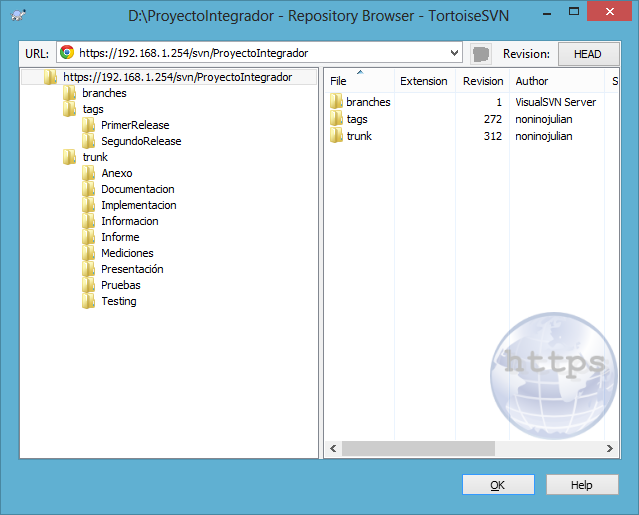
\includegraphics[width=0.8\linewidth,keepaspectratio]{./introduccion//img/intro01}
				\caption{Esquema de directorios del repositorio SVN}
				\label{fig:intro01}
			\end{figure}
			
			Como se observa, los tres directorios principales del repositorio son:
			\begin{itemize}
			  	\item \emph{branches}: Donde se guardar�n todas las ramas del repositorio.
			  	\item \emph{tags}: En �ste directorio se almacenan las etiquetas que se le han asignado a 
			  		algunas versiones del proyecto. En �ste caso, se utilizan dos etiquetas \emph{Primer Release}
			  		y \emph{Segundo Release}.
			  	\item \emph{trunk}: Aqu� se almacena la copia de trabajo con la que est� trabajando el desarrollador.
			\end{itemize}
			
			\begin{figure}[H]
				\centering
				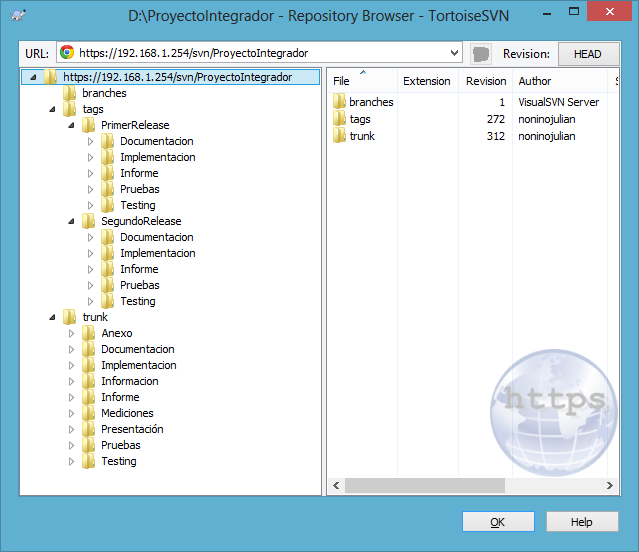
\includegraphics[width=1\linewidth,keepaspectratio]{./introduccion//img/intro02}
				\caption{Esquema de directorios del repositorio SVN (m�s detallado)}
				\label{fig:intro02}
			\end{figure}
			
			
			
		
 		% Marco te�rico
 			\part{Marco Te�rico}
 				% Redes de Petri
 					%%%%%%%%%%%%%%%%%%%%%%%%%%%%%%%%%%%%%%%%%%%%%%%%%%%%%%%%%%%%%%%%%%%%%%%%%%%%%%%%%%%%%
%																					%
%	TRABAJO: Proyecto Integrador													%
%																					%
%		Titulo: 	Desarrollo de IP cores con procesamiento de Redes de Petri 		%
%					Temporales para sistemas multicore en FPGA						%
%																					%
%		Autores:	Juli�n Nonino													%
%					Carlos Renzo Pisetta											%
%		Director:	Orlando Micolini												%
%																					%
%	Parte: Marco Te�rico															%
%	Capitulo: Redes de Petri														%	
%	Archivo: chap_redes_de_petri.tex												%
%																					%
%%%%%%%%%%%%%%%%%%%%%%%%%%%%%%%%%%%%%%%%%%%%%%%%%%%%%%%%%%%%%%%%%%%%%%%%%%%%%%%%%%%%%

% Path Imagenes: ./marco_teorico/redes_de_petri/img
% Nombre predeterminado imagenes: petrixx
%	xx es el numero de imagen

\chapter{Redes de Petri}
	\label{chap:chap_redes_de_petri}

	En este cap�tulo se realizar� una introducci�n a las Redes de Petri, explicando los elementos que la componen,
	sus propiedades, el grafo de alcanzabilidad de marcados, invariantes de plazas y transiciones, trampas y sifones.
	Tambi�n, se muestra la ecuaci�n de estado de una Red de Petri y c�mo es posible ejecutar la red a partir de ella.
	Luego, se presentar�n extensiones que permiten formar las Redes de Petri con Arcos Inhibidores, y las Redes de 
	Petri Temporales. Para estas �ltimas, se detallar�n las dos sem�nticas de tiempo posibles, Redes de Petri con 
	Tiempo y Redes de Petri Temporizadas.

	El objetivo de este cap�tulo es instruir brevemente al lector sobre Redes de Petri, brindando los conocimientos 
	b�sicos para la comprensi�n de otros cap�tulos de este trabajo.
	
	% Introduccion
		%%%%%%%%%%%%%%%%%%%%%%%%%%%%%%%%%%%%%%%%%%%%%%%%%%%%%%%%%%%%%%%%%%%%%%%%%%%%%%%%%%%%%
%																					%
%	TRABAJO: Proyecto Integrador													%
%																					%
%		Titulo: 	Desarrollo de IP cores con procesamiento de Redes de Petri 		%
%					Temporales para sistemas multicore en FPGA						%
%																					%
%		Autores:	Juli�n Nonino													%
%					Carlos Renzo Pisetta											%
%		Director:	Orlando Micolini												%
%																					%
%	Parte: Marco Teorico															%
%	Capitulo: Redes de Petri														%
%	Seccion: Introduccion															%	
%	Archivo: introduccion.tex														%
%																					%
%%%%%%%%%%%%%%%%%%%%%%%%%%%%%%%%%%%%%%%%%%%%%%%%%%%%%%%%%%%%%%%%%%%%%%%%%%%%%%%%%%%%%

% Path Imagenes: ./marco_teorico/redes_de_petri/img
% Nombre predeterminado imagenes: petrixx
%	xx es el numero de imagen

\section{Introducci�n}
	\label{sec:introduccion_petri}

	Una Red de Petri o Petri Net es un modelo gr�fico, formal y abstracto para describir y analizar el flujo de 
	informaci�n. Conforma una herramienta matem�tica que puede aplicarse especialmente a los sistemas paralelos 
	que requieran simulaci�n y modelado de la concurrencia en los recursos compartidos. Las Redes de Petri (PN) 
	est�n asociadas con la teor�a de grafos y se pueden considerar como aut�matas formales y generadores de 
	lenguajes formales \cite{diaz_petri}.
		
	Las Redes de Petri constan de cuatro componentes fundamentales.
	\begin{itemize}
		\item \textbf{Plazas}: Las plazas de una Red de Petri, permiten representar el estado del sistema. 
			Podr�an definirse como variables de estado que toman valores enteros (cantidad de \emph{tokens}).
			Se representan con un c�rculo.
		\item \textbf{Transiciones}: Son representadas con un rect�ngulo. Representan el conjunto de sucesos
			que hacen que el estado del sistema cambie.
		\item \textbf{Arcos}: Los arcos indican las conexiones entre lugares y transiciones. Nunca unen dos 
			lugares o dos transiciones en forma sucesiva. Pueden entrar o salir varios arcos de una misma 
			transici�n o de un mismo lugar.
			Los arcos tienen asociado un \emph{peso} que indica la cantidad de tokens que se consumen o generan al 
			atravesarlo. El disparo de una transici�n retira tantos tokens de cada uno de sus lugares de entrada 
			como lo indican los pesos de los arcos conectores y a�ade los tokens a sus lugares de salida como lo 
			indican los pesos de los arcos de salida.
		\item \textbf{Tokens}: Los tokens representan el valor espec�fico de la condici�n o estado. Son graficados 
			como un punto negro, un n�mero natural o cero dentro de una plaza.
	\end{itemize}

	La \ref{fig:Petri01} muestra c�mo son representados en el grafo de una Red de Petri los conceptos antes mencionados.
	\begin{figure}[H]
		\centering
		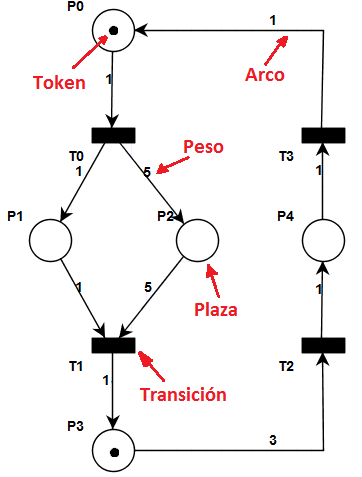
\includegraphics[width=.35\linewidth]{./marco_teorico/redes_de_petri/img/Petri01}
		\caption{Ejemplo de Red de Petri}
		\label{fig:Petri01}
	\end{figure}

	\subsection{Estructura de una Red de Petri}
		Una Red de Petri Marcada queda definida como una 5-tupla de la siguiente manera:
		\begin{center}
			$PN = \{P, T, I^-, I^+, m_0\}$ 
		\end{center}
		Donde:
		\begin{itemize}
			\item $\boldsymbol{P = \{p_1, p_2, p_3 \ldots p_m\}}$, conjunto de $m$ lugares con $m$ finito y 
				distinto de cero.
				Para el ejemplo de la \ref{fig:Petri01} la cantidad de plazas es cinco y se
				tiene que: ${P = \{p_1, p_2, p_3, p_4, p_5\}}$
			\item $\boldsymbol{T = \{t_1, t_2, t_3 \ldots t_n\}}$, conjunto de $n$ transiciones con $n$ finito y 
				distinto de cero. En el ejemplo de la Figura \ref{fig:Petri01} hay cuatro transiciones y se 
				tiene que: ${T = t_1, t_2, t_3\}}$
			\item \textbf{$\boldsymbol{I}$, matriz de incidencia}. Esta matriz es de dimensiones $m�n$, representa los pesos
			 	de los arcos, siendo sus valores positivos cuando el arco va desde una transici�n hacia una plaza 
			 	y negativos los inversos.
				As� mismo esta matriz de incidencia debe separarse en dos para representar la estructura. Estas dos 
				matrices son:
				\begin{description}
					\item [$\boldsymbol {I-}$] Matriz de incidencia negativa. Esta matriz es de dimensiones $m�n$, 
						representa los pesos de los arcos que ingresan desde los lugares de P a las transiciones 
						de T.
					\item [$\boldsymbol {I+}$] Matriz de incidencia positiva. Esta matriz es de dimensiones $m�n$, 
						representa los pesos de los arcos que salen desde las transiciones de T hacia los lugares 
						de P. 
					\end{description}
				Para una red con $m$ plazas y $n$ transiciones, la matriz de incidencia es de tama�o $m�n$, sus 
				elementos $a_{ij}$ son:
				\begin{equation}
					\begin{matrix}
						\forall p_i \in P \wedge \forall t_j\in T \Rightarrow a_{ij}=\;
						\begin{cases} 
							\begin{matrix} 	0 		& si \; entre \; p_i \; y \; t_j\\ 
					 						  		&	 \;	no \; existen\; arcos\\
											W_{ij} 	& si \; p_i \; es \; plaza\\
												 	& de \; salida \; de \; t_j\\
											-W_{ij} & si \; p_i\; es \; plaza\\
											 		& de \; entrada \; de \; t_j 
							\end{matrix}
						\end{cases}
					\end {matrix}
					\label{eq:definicionincidencia}
				\end{equation}
				
				Para la red de la Figura \ref{fig:Petri01} la matriz de incidencia tiene la siguiente forma
				
				\begin{center}
					\begin{tabular}{c c}
						%Primer fila - Columna 1
							$I^+ = \begin{bmatrix}
 						  				0 & 0 & 0 & 1 \\
 						  				1 & 0 & 0 & 0 \\
   						  				5 & 0 & 0 & 0 \\
   						  				0 & 1 & 0 & 0 \\
   						  				0 & 0 & 1 & 0 \\
   									\end{bmatrix}$
   						&
   						%Primer fila - Columna 2
							$I^- = \begin{bmatrix}
 						  				1 & 0 & 0 & 0 \\
 						  				0 & 1 & 0 & 0 \\
   						  				0 & 5 & 0 & 0 \\
   						  				0 & 0 & 3 & 0 \\
   						  				0 & 0 & 0 & 1 \\
   									\end{bmatrix}$
   				 		\\
   				 		Matriz de incidencia positiva & Matriz de incidencia negativa
   				 		\\
   				 		\\
						% Segunda fila
						\multicolumn{2}{c}
						{	$I = \begin{bmatrix}
 						  			-1 & 0 & 0 & 1 \\
 						  			1 & -1 & 0 & 0 \\
   						  			5 & -5 & 0 & 0 \\
   						  			0 & 1 & -3 & 0 \\
   						  			0 & 0 & 1 & -1 \\
   								\end{bmatrix}$  
   						}
						\\
						\multicolumn{2}{c}{Matriz de incidencia}
					\end{tabular}
				
				\end{center}
						
			\item $\boldsymbol {m_0}$ es el \textbf{marcado inicial} de la red, un vector de asignaci�n de 
				tokens a las plazas de la red, de esta forma se define la configuraci�n inicial de los tokens 
				de la red. Por ejemplo puede definirse el marcado de una plaza como $m(i)$, esto indica la 
				cantidad de tokens ubicados en la plaza $i$.
		 		Para el ejemplo anterior, resulta: $m_0 = \begin{bmatrix}
 						  									1 & 0 & 0 & 1 & 0
 						  									\end{bmatrix}^T$
		\end{itemize}
	
	\subsection{Ejecuci�n de una Red de Petri}
	
		El comportamiento din�mico de una red de Petri est� definido por la sensibilizaci�n y el disparo 
		de sus transiciones.
	
		\subsubsection{Transici�n sensibilizada}
			Se dice que una transici�n $t_j$ est� sensibilizada si y s�lo si todas las plazas de entrada a la 
			transici�n tienen una cantidad de tokens igual o mayor al peso indicado por el arco que la une con 
			la transici�n.
			Formalmente:
			\begin{equation}
				\forall p_i\in I^-(t_j)/ m(p_i)\geq W_{ij}
				\label{eq:transiciion_sensibilizada}
			\end{equation}
			
			Siendo $W_{ij}$ el peso del arco que une la plaza $i$ con la transici�n $j$.				
		
		\subsubsection{Disparo de una transici�n}
		
			El disparo de una transici�n es lo que provoca que el estado (marcado) de una Red de Petri cambie. 
			La funci�n disparo (d) de una transici�n $t_j$  se define de la siguiente manera.
			\begin{equation}
				\begin{matrix}
					d(m_k,t_j )\Rightarrow m_{k+1} (p_i)= \;
					\begin{cases} 
						\begin{matrix} 	m_k (p_i )-W_{ij} & \forall p_i \in I^-(t_j)\\
										m_k (p_i )+W_{ij} & \forall p_i \in I^+(t_j)\\
										m_k (p_i ) & para\; el\; resto\; de\; los\; casos 
						\end{matrix}
					\end{cases}
				\end {matrix}
				\label{eq:disparo}
			\end{equation}
			Donde:
			\begin{itemize}
			  	\item $m_k$ es el marcado actual de la red 
  			  	\item $m_{k+1}$ es el marcado que tomara la red luego del disparo.
  			  	\item $W_{ij}$ son los elementos de la matriz de incidencia \emph{I}.
			\end{itemize}
					
		\subsubsection{Ecuaci�n de estado de una Red de Petri}
			\label{subsubsec:ecuacion_estado_petri}
			
			La ecuaci�n de estado determina el estado de la Red de Petri a cada instante, queda definida a 
			partir de la matriz de incidencia y un vector de disparo que indica la transici�n o transiciones 
			que deben ser disparadas.
			\begin{equation}
				m_{k+1} = m_k + I � d_k
				\label{eq:ecuacion_estado_uno}
			\end{equation}
			
			Siendo $d$, un vector cuya dimensi�n es la cantidad de transiciones y su funci�n, indicar cu�l o 
			cu�les transiciones se desean disparar.
			
			Si se parte desde el marcado inicial $m_0$, se puede aplicar sucesivamente la ecuaci�n de estado para 
			llegar al estado $i$. De �sta manera, se deduce la siguiente ecuaci�n:
			\begin{equation}
				m_i = m_0 + I � \sum_{k=1}^{i} d_k
				\label{eq:ecuacion_estado_dos}
			\end{equation}
				
	
	
	% Propiedades de las Redes de Petri
		%%%%%%%%%%%%%%%%%%%%%%%%%%%%%%%%%%%%%%%%%%%%%%%%%%%%%%%%%%%%%%%%%%%%%%%%%%%%%%%%
%	TRABAJO: Proyecto Integrador
%		Titulo: 	Desarrollo de IP cores con procesamiento de Redes de Petri 	
%					Temporales para sistemas multicore en FPGA					
%		Autores:	Juli�n Nonino												%					Carlos Renzo Pisetta										%		Director:	Orlando Micolini											
%%%%%%%%%%%%%%%%%%%%%%%%%%%%%%%%%%%%%%%%%%%%%%%%%%%%%%%%%%%%%%%%%%%%%%%%%%%%%%%%

% Path im�genes: ./marco_teorico/redes_de_petri/img
% Nombre predeterminado im�genes: petrixx
%	xx es el numero de imagen

\section{Propiedades de las Redes de Petri}
	\label{sec:propiedades_petri}

	Las Redes de Petri tienen propiedades especiales que se detallar�n a continuaci�n.
	
	\subsection{Redes de Petri limitadas}
		
		Sea la Red de Petri $PN = {P, T, I^-, I^+, m_0}$, se dice que una plaza $p$ es \textbf{\emph{k-limitada}} si existe un valor $k$ tal que para todo marcado $m$ perteneciente al conjunto de marcados de la Red de Petri $PN$ se cumple que el valor de marcado de la plaza $p$ es menor o igual que $k$.
		\begin{equation}
			\exists k / \forall m \in marcados(PN) : m(p) \leq k
			\label{eq:red_limitada}
		\end{equation}
		
		El arreglo $marcados(PN)$ representa todos los marcados posibles de la Red de Petri. Se dice que una Red de Petri es \emph{k-limitada} si todas sus plazas son \emph{k-limitadas}.
		
	\subsection{Redes de Petri seguras}
	
		Se dice que una red de Petri PN es \textbf{\emph{segura}} si y s�lo si todas sus plazas son \textbf{\emph{1-limitadas}}. Esto implica que una transici�n no puede ser disparada si alguna de sus plazas de llegada est� ocupada.
		
	\subsection{Redes de Petri c�clicas}
			
		Se dice que una Red de Petri es \textbf{\emph{c�clica}} si existe siempre una sucesi�n de marcados que lleve desde cualquier marcado $m$ al marcado inicial $m_0$.
	
	\subsection{Redes de Petri repetitivas}

		Se dice que una Red de Petri es \textbf{\emph{repetitiva}} si existe siempre una secuencia de disparos que lleve desde un marcado $m$ hasta el mismo marcado $m$.

	\subsection{Redes de Petri conservativas}

		Una Red de Petri es \textbf{\emph{conservativa}} si se cumple que para todo marcado $m$ perteneciente al conjunto de marcados de la red, la cantidad de marcas de $m$ es igual a la cantidad de marcas de $m_0$. Es decir, se conserva la cantidad de tokens.

	\subsection{Propiedad de vivacidad (liveness)}

		Se dice que una Red de Petri esta \textbf{\emph{viva}} si y s�lo si en todo momento sus transiciones pueden ser disparadas o si existe una secuencia de disparos v�lidos que lleven a que la transici�n pueda dispararse. 

	\subsection{Propiedades de bloqueo (deadlock)}
	
		Un \textbf{\emph{bloqueo}} en una Red de Petri implica que una transici�n nunca podr� ser disparada independientemente de la secuencia de disparos que se aplique. Recordando la propiedad anterior, se puede decir que una Red de Petri viva garantiza la ausencia de bloqueos. Este concepto est� sustentado en la ausencia de \emph{marcados sumideros}. Un marcado sumidero es aquel marcado a partir del cual ninguna transici�n puede ser disparada.
		
	\subsection{Alcanzabilidad}

		La alcanzabilidad determina si un marcado $m$ es alcanzable desde un marcado inicial $m_0$, es decir, determina si $m$ pertenece al conjunto de marcados de la Red de Petri. Se dice que un marcado $m$ es alcanzable desde $m_0$ si y s�lo si existe una secuencia de disparos que lleven desde $m_0$ hasta $m$. Para determinar si un marcado $m$ es alcanzable, se utiliza la ecuaci�n de estado de una Red de Petri de la siguiente manera:
		\begin{equation}
			m = m_0 + I � \sigma
			\label{eq:alcanzabilidad}
		\end{equation}
		D�nde $\sigma$ es una secuencia de disparos.
				
		Si no fuera posible encontrar una secuencia de disparos, se dice que el marcado $m$ es \emph{inalcanzable}. Si existieran m�ltiples soluciones, es decir, varias secuencias de disparos posibles para alcanzar el marcado $m$, se dice que la Red de Petri se comporta de manera \emph{NO determin�stica}. Hay que notar que la soluci�n de la ecuaci�n no indica el orden en que las transiciones deben ser disparadas, por lo que, �ste debe ser encontrado ejecutando todas las secuencias posibles. Por ello, es posible que a pesar de encontrar una secuencia de disparos, no exista un ordenamiento de los mismos que permita alcanzar la marca $m$ y sea aplicable a la Red de Petri en cuesti�n.
		
		\subsubsection{Grafo de alcanzabilidad}
				
			El grafo de alcanzabilidad de una Red de Petri representa el conjunto de todos los marcados alcanzables desde el marcado inicial $m_0$. Consiste en un grafo en forma de �rbol en el que cada nodo es un marcado alcanzable de la red y se conectan mediante arcos etiquetados con la transici�n que se dispara para pasar de un marcado a otro.
			
			Partiendo del estado inicial $m_0$ se generan todos los estados alcanzables desde �ste mediante un disparo de cada una de las transiciones sensibilizada. A partir de cada estado, se vuelve a repetir el proceso, apareciendo, en consecuencia, un grafo en forma de �rbol que representa todos los estados del sistema.
			
			Por ejemplo, sea la siguiente Red de Petri, se plantear� el grafo de alcanzabilidad de la misma.
				
			\begin{figure}[H]
				\centering
				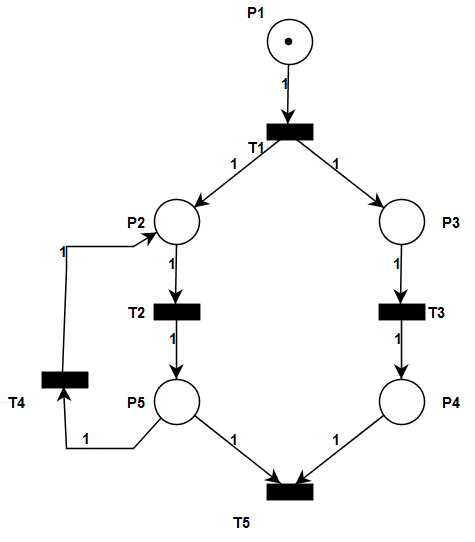
\includegraphics[width=0.5\linewidth]{./marco_teorico/redes_de_petri/img/Petri02}
				\caption{Red de Petri de Ejemplo para Grafo de alcanzabilidad}
				\label{fig:Petri02}
			\end{figure}
				
			El grafo de alcanzabilidad de la red de la Figura \ref{fig:Petri02}, comenzar�a de la siguiente manera:
			\begin{figure}[H]
				\centering
				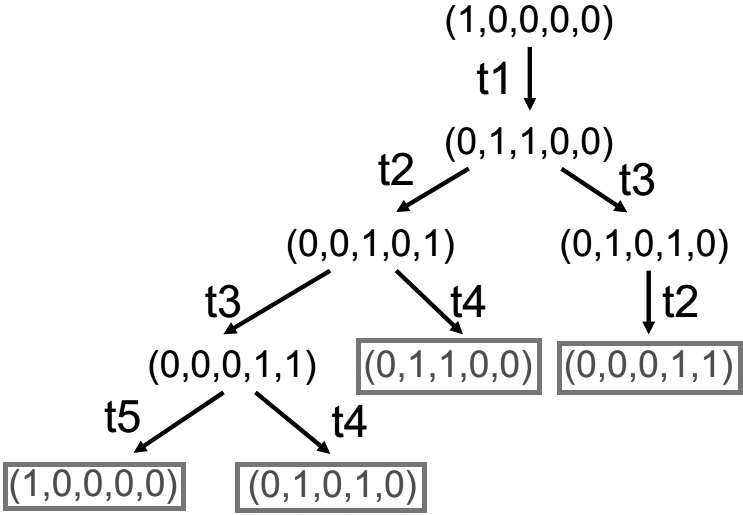
\includegraphics[width=0.65\linewidth]{./marco_teorico/redes_de_petri/img/Petri03}
				\caption{Ejemplo de grafo de alcanzabilidad}
				\label{fig:Petri03}
			\end{figure}
			El proceso se detiene en los marcados repetidos, que en la Figura \ref{fig:Petri03} aparecen recuadrados.

	
	% An�lisis estructural de Redes de Petri
		%%%%%%%%%%%%%%%%%%%%%%%%%%%%%%%%%%%%%%%%%%%%%%%%%%%%%%%%%%%%%%%%%%%%%%%%%%%%%%%%
%	TRABAJO: Proyecto Integrador
%		Titulo: 	Desarrollo de IP cores con procesamiento de Redes de Petri 	
%					Temporales para sistemas multicore en FPGA					
%		Autores:	Juli�n Nonino												%					Carlos Renzo Pisetta										%		Director:	Orlando Micolini											
%%%%%%%%%%%%%%%%%%%%%%%%%%%%%%%%%%%%%%%%%%%%%%%%%%%%%%%%%%%%%%%%%%%%%%%%%%%%%%%%

% Path im�genes: ./marco_teorico/redes_de_petri/img
% Nombre predeterminado im�genes: petrixx
%	xx es el numero de imagen

\section{An�lisis estructural de Redes de Petri}
	\label{sec:analisis_estructural}

	Las propiedades de una Red de Petri pueden ser demostradas construyendo el grafo de alcanzabilidad de la misma. Sin embargo, el tama�o de este grafo crece exponencialmente con el n�mero de plazas.
	
	El an�lisis estructural de una Red de Petri, hace posible demostrar algunas de las propiedades de la red sin necesidad de realizar el grafo de alcanzabilidad.
	
	Existen dos t�cnicas principales, los \textbf{invariantes} y las \textbf{trampas (traps)}.
	
	\subsection{Invariantes de plazas y transiciones}
		\label{subsec:invariantes}
	
		\subsubsection{Definiciones}
			
			El efecto de una secuencia de disparos en la ecuaci�n  de estado de una Red de Petri est� determinado por la matriz de incidencia $I$ y el vector de ocurrencias de transiciones en la secuencia de disparo.
			
			Sea $\sigma\in T^*$ una secuencia de disparos que lleva a una Red de Petri desde el estado $m$ hasta el estado $m_{i+1}$ entonces se puede decir que:
			\begin{itemize}
  				\item La secuencia $\sigma$ tiene asociado un vector $\vec{\sigma}\in \mathbb{N}^T$ (siendo $T$ la cantidad de transiciones de la red) llamado vector de ocurrencia tal que $\vec{\sigma}$ representa la cantidad de ocurrencias de $t$ en la secuencia $\sigma$.
	  			\item La ecuaci�n de estado resulta:
	  					\begin{equation*}
	  						m_(i+1) = m_i + I � \vec{\sigma}
	  					\end{equation*}
				\end{itemize}
			
		\subsubsection{Invariantes}		
			
			Con la ayuda de la ecuaci�n anterior, se buscan cantidades invariantes que permitan analizar estructuralmente a la Red de Petri. En particular, se trabajar� con los canceladores de la matriz de incidencia $I$.
			
			Sea $P$ la cantidad de plazas de una Red de Petri y $T$ la cantidad de transiciones, las cancelaciones de la matriz $I$ generan cuatro vectores:
			\begin{itemize}
				\item \underline{P-flow}
			  		\\
				  	Es un vector no nulo $ x\in \mathbb{Z}^P$ que satisface la siguiente ecuaci�n:
				  	\begin{equation}
						x^t � I = \vec{0} 
						\label{eq:pflow}
					\end{equation} 
					
				\item \underline{P-semiflow}
					\\
				  	Es un vector no nulo $ x\in \mathbb{N}^P$ que satisface la siguiente ecuaci�n:
				  	\begin{equation}
						x^t � I = \vec{0} 
						\label{eq:psemiflow}
					\end{equation}
				\item \underline{T-flow}
					\\
				  	Es un vector no nulo $ u\in \mathbb{Z}^P$ que satisface la siguiente ecuaci�n:
				  	\begin{equation}
						u^t � I = \vec{0} 
						\label{eq:tflow}
					\end{equation} 
				\item \underline{T-semiflow}
					\\
				  	Es un vector no nulo $ u\in \mathbb{N}^P$ que satisface la siguiente ecuaci�n:\\
				  	\begin{equation}
						u^t � I = \vec{0} 
						\label{eq:tsemiflow}
					\end{equation}
			\end{itemize}
  
			Un vector \textbf{P-flow} es una suma ponderada de las plazas con coeficientes enteros. Provee una transformaci�n desde el marcado de un conjunto de plazas a un n�mero entero.
						
			Un \textbf{P-semiflow} es una suma ponderada de las plazas con coeficientes naturales.
						
			Los vectores P-flow y P-semiflow son llamados \textbf{invariantes de plazas} o \textbf{P-invariantes}.
			\\
			
			Los \textbf{T-semiflows} pueden ser obtenidos como el vector de ocurrencia de una secuencia de disparos, mientras que los \textbf{T-flows} pueden ser obtenidos a partir de la diferencia entre dos vectores de ocurrencia.
			
			Los vectores T-flow y T-semiflow son llamados \textbf{invariantes de transiciones} o \textbf{T-invariantes}.
			\\
			
			\begin{raggedright}
				\textbf{\emph{Proposiciones}}
			\end{raggedright}
			
			\begin{enumerate}
  				\item Sea $x$ un vector \emph{P-flow} y $\sigma$ una secuencia de disparos que lleva desde el estado $m_i$ hasta el estado $m_{i+1}$ entonces:
  					\begin{equation}
						x^t � m_i = x^t � m_{i+1} 
						\label{eq:efectopflow}
					\end{equation}
					
					Esto se demuestra con la ecuaci�n de estado:
  						\begin{equation*}
  							\begin{array}{c}
  								 m_{i+1} = m_i + I � \vec{\sigma}
  								 \\
  								 x^t � m_{i+1} = x^t � (m_i + I � \vec{\sigma})
  								 \\
  								 x^t � m_{i+1} = x^t � m_i + x^t � I �\vec{\sigma}
  							\end{array}
  						\end{equation*}	
  					
  					Luego, como $x^t � I = \vec{0}$ entonces:
  						\begin{equation*}
  							x^t � m_{i+1} = x^t � m_i
  						\end{equation*}
  				
  				\item Sea $u$ un vector \emph{T-semiflow} y $\sigma$ una secuencia de disparos tal que 
  					$\sigma = u$, entonces:
  					\begin{equation}
						m_i\xrightarrow{\;\sigma\;} m_{i+1}\Rightarrow m_i = m_{i+1}
						\label{eq:efectopsemiflow}
					\end{equation}
					
					En otras palabras, $\sigma$ es una secuencia repetitiva y estacionaria.
					
					La afirmaci�n anterior se demuestra con la ecuaci�n de estado de la siguiente manera:
	  					\begin{equation*}
	  						m_{i+1} = m_i+I � \vec{\sigma}
	  					\end{equation*}
  					
  					Dado que $\vec{\sigma} = u$\\
	  					\begin{equation*}
	  						m_{i+1} = m_i + I � u
	  					\end{equation*}
  					
  					Luego, como $I � u = \vec{0}$ entonces:
  					\begin{equation*}
  						m_{i+1} = m_i
  					\end{equation*}
  						
  				\item Sea $u$ un vector \emph{T-flow} y $\sigma_1$ y $\sigma_2$ dos secuencias de disparos tal que $\sigma_1 - \sigma_2 = u$, entonces:
  					\begin{equation}
						m\xrightarrow{\;\;\sigma_1\;\;} m' 
						\wedge 
						m\xrightarrow{\;\;\sigma_2\;\;} m''
						\Rightarrow
						m' = m''
						\label{eq:efectotsemiflow}
					\end{equation}
					
					Con la ecuaci�n de estado, se demuestra la proposici�n anterior de la siguiente forma:
					\begin{equation*}
						m' = m + I � \vec{\sigma_1}
						m'' = m + I � \vec{\sigma_2}
					\end{equation*}
					
					Haciendo:
					\begin{equation*}
						\begin{array}{c}
							m' - m'' = (m + I � \vec{\sigma_1}) - (m + I � \vec{\sigma_2}) \\
							m' - m'' = m + I � \vec{\sigma_1} - m - I � \vec{\sigma_2} \\
							m' - m'' = I � \vec{\sigma_1} - I � \vec{\sigma_2} \\
							m' - m'' = I � (\vec{\sigma_1} - \vec{\sigma_2}) 
						\end{array}
					\end{equation*}
					
					Dado que $\vec{\sigma_1} - \vec{\sigma_2} = u$
					\begin{equation*}
						m' - m'' = I � u	
					\end{equation*}							 
  					
  					Luego, como $ I � u = \vec{0}$ entonces
  					\begin{equation*}
  						m' - m'' = \vec{0}
  					\end{equation*}	
			\end{enumerate}
			
		\subsubsection{Invariantes de Transiciones}
			
			Los vectores \emph{T-flow} y los \emph{T-semiflow} son \textbf{invariantes de transiciones} o \textbf{T-invariantes}. En particular, los vectores \emph{T-semiflow} indican posibles bucles (loops) en la red. Es decir, una secuencia de disparos que tenga asociado un invariante de transici�n, vuelve al mismo marcado desde el que parti�. Por ejemplo, sea la siguiente Red de Petri, el vector:
			\begin{figure}[H]
				\begin{minipage}{0.5\textwidth}
					\centering 
					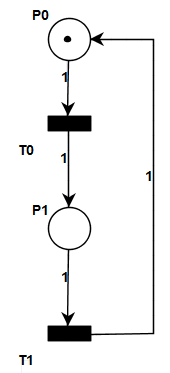
\includegraphics[width=0.3\textwidth]{./marco_teorico/redes_de_petri/img/Petri04}
					\caption{Ejemplo para T-invariantes} 
					\label{fig:ej_tinv}
				\end{minipage}
				\hfill
				\begin{minipage}{0.5\textwidth}
					\begin{center}
						$u=\begin{bmatrix}
		 					1 \\
		 					1
		 				\end{bmatrix}$\\
		 			\end{center}
		 			es un invariante de transiciones. Esto se demuestra con la ecuaci�n de estado de la red.
						\begin{center}
							$m=m_0+I�u$\\[3mm]
							$m=\begin{bmatrix}
					 				1 \\
					 				0
					 	   		\end{bmatrix}
					 	   	+ \begin{bmatrix}
					 				-1 &  1 \\
					 				1 & -1
					 			\end{bmatrix}
							� \begin{bmatrix}
					 				1\\
					 				1
					 			\end{bmatrix}$
					 		\\[3mm]
					 		$m=\begin{bmatrix}
					 				1 \\
					 				0
					 			\end{bmatrix}
					 		+  \begin{bmatrix}
					 				0 \\
					 				0
					 		   \end{bmatrix} 
					 		=  \begin{bmatrix}
					 				1 \\
					 				0
					 			\end{bmatrix}$\\	
						\end{center}					 
				\end{minipage}
			\end{figure}
									
		\subsubsection{Invariantes de plazas (p-invariantes)}
			
			Sea una Red de Petri $PN(I, m_0)$ definida por una estructura de red $I$ y un marcado inicial $m_0$, si $x$ es un vector \emph{P-flow} o un \emph{P-semiflow}, se cumple que:
			\begin{equation}
				\forall m \in marcados de PN: x^t � m = x^t � m_0
			\end{equation}
			
			Para todo marcado $m$ perteneciente al conjunto de marcados de la red $PN$ se cumple que el producto de la transpuesta del vector $x$ por cualquier marcado, se mantiene igual al producto con el marcado inicial $m_0$. 
			
			Si el vector $x$ es \emph{P-semiflow}, se dice que $x$ es un \textbf{\emph{invariante positivo}}.
			
			Los invariantes positivos tienen muchas aplicaciones. Por ejemplo, todas las plazas que est�n incluidas en un vector P-invariante se encuentran limitadas al valor de marcado que sumaban al inicio.
			
			Tambi�n, los invariantes de plazas pueden ser utilizados para identificar los estados de los procesos modelados con la Red de Petri y adem�s, para verificar situaciones de exclusi�n mutua. En las Redes de Petri que se presentan a continuaci�n, se ejemplificar�n las aplicaciones antes mencionadas.
			
			Se plantea la Red de Petri de un sistema productor consumidor con un buffer de capacidad limitada.
			\begin{figure}[H]
				\centering
				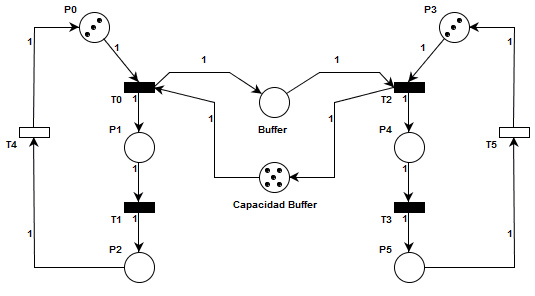
\includegraphics[width=.7\linewidth]{./marco_teorico/redes_de_petri/img/Petri05}
				\caption{Red de Petri para problema Productor-Consumidor}
				\label{fig:Petri05}
			\end{figure}
			
			Los invariantes de plazas pueden ser escritos como ecuaciones que muestran propiedades de la Red de Petri. 
			
			En este ejemplo, los vectores \emph{P-invariantes} son\footnote{Los vectores han sido calculados utilizando la Ecuaci�n \ref{eq:pflow} y la Ecuaci�n \ref{eq:psemiflow}}:
			
			\begin{center}
				\begin{tabular}{c c c c c c c c c}
						& P0	& P1 	& P2 	& P3 	& P4 	& P5 	& Capacidad Buffer 	& Buffer
					\\
					\hline
					1)  & 0 	& 0 	& 0 	& 0 	& 0 	& 0 	& 1 				& 1
					\\
					\hline
					2) 	& 1 	& 1 	& 1 	& 0 	& 0 	& 0 	& 0 				& 0
					\\
					\hline
					3) 	& 0 	& 0 	& 0 	& 1 	& 1 	& 1 	& 0 				& 0\\
					\hline
				\end{tabular}
			\end{center}
			
			Traducidos a ecuaciones resultan:
			\begin{enumerate}
  				\item $M(Capacidad Buffer) + M(Buffer) = 5$
  					\\
					En esta ecuaci�n que se deriva del primer vector \emph{P-invariante}, se puede ver como la cantidad de marcas que se encuentran ubicadas entre las plazas \emph{Capacidad Buffer} y \emph{Buffer}, se mantiene constante. Esto indica, que est�n limitadas.
				\item $M(P0) + M(P1) + M(P2) = 3$
					\\
					Desde el segundo vector \emph{P-invariante}, se obtiene la ecuaci�n anterior. Por esta ecuaci�n, deducimos que las plazas $P0$, $P1$ y $P2$ representan los estados de un proceso. Dado que la cantidad de tokens entre ellas se mantiene constante, esto permite deducir que los tokens van cambiando de estado. Este proceso, se corresponde con el proceso \emph{Productor}.
				\item $M(P3) + M(P4) + M(P5) = 3 $
					\\
					�dem al caso anterior, el hecho de que el numero de tokens se mantenga en las plazas $P3$, $P4$ y $P5$ permite identificar los estados del otro proceso modelado, el proceso \emph{Consumidor}.
			\end{enumerate}
				
			Si el buffer del ejemplo anterior, tuviera que ser accedido con exclusi�n mutua, el modelado del sistema con una Red de Petri resultar�a de la siguiente manera.
			\begin{figure}[H]
				\centering
				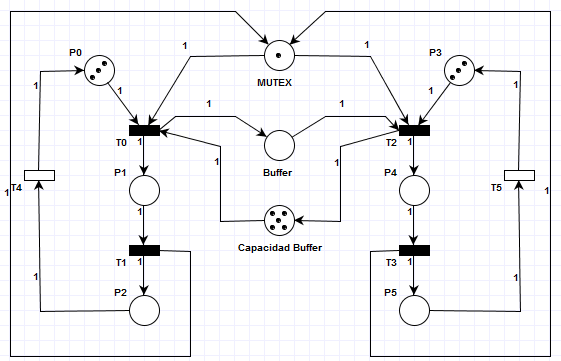
\includegraphics[width=.7\linewidth]{./marco_teorico/redes_de_petri/img/Petri06}
				\caption{Red de Petri para problema Productor-Consumidor con Exclusi�n Mutua}
				\label{fig:Petri06}
			\end{figure}
				
			Obteniendo los vectores \emph{P-invariantes} del sistema se tiene:
			\begin{center}
				\begin{tabular}{c c c c c c c c c c}
						& P0 	& P1 	& P2 	& P3 	& P4 	& P5 	& Capacidad Buffer 	& Buffer 	& MUTEX
					\\
					\hline  
					1) 	& 0 	& 0 	& 0 	& 0 	& 0 	& 0 	& 1 				& 1 		& 0
					\\
					\hline
					2) 	& 1 	& 1 	& 1 	& 0 	& 0 	& 0 	& 0 				& 0 		& 0
					\\
					\hline
					3) 	& 0 	& 0 	& 0 	& 1 	& 1 	& 1 	& 0 				& 0 		& 0
					\\
					\hline
					4) 	& 0 	& 1 	& 0 	& 0 	& 1 	& 0 	& 0 				& 0 		& 1
					\\
					\hline
				\end{tabular}
			\end{center}	
			
			Como se puede notar, se obtuvo un cuarto invariante de plazas adem�s de los que ya aparec�an en el ejemplo anterior. La ecuaci�n de este cuarto invariante es:
			\begin{equation*}
				M(P1) + M(P4) + M(MUTEX) = 1
			\end{equation*}
 
 			Las plazas $P1$ y $P4$ se corresponden con los estados de procesos \emph{Produciendo} y \emph{Consumiendo} respectivamente. El hecho de que aparezcan en un invariante junto con la plaza \emph{MUTEX} indica que la cantidad de tokens entre estas tres plazas no cambia. Dado que el valor constante es \emph{1}, �ste \emph{P-invariante} muestra la exclusi�n mutua entre ambos procesos.
				
	\subsection{Trampas (Traps)}
		\label{subsec:traps}
			
		Para explicar que es un \textbf{\emph{trap}} se presentar� una Red de Petri de ejemplo \cite{muscholl}.
		\begin{figure}[H]
			\centering
			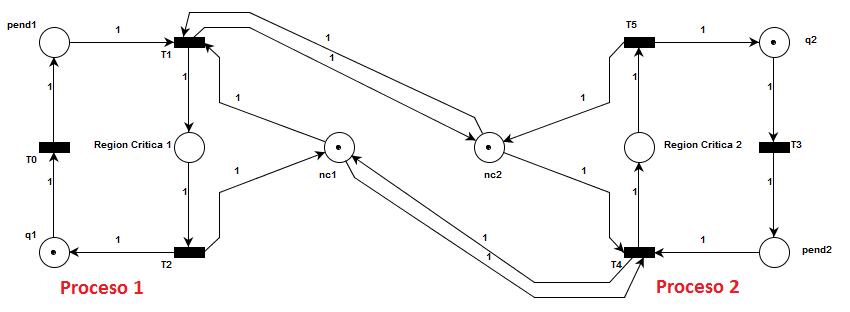
\includegraphics[width=1\linewidth]{./marco_teorico/redes_de_petri/img/Petri07}
			\caption{Ejemplo red de Petri con Traps}
			\label{fig:Petri07}
		\end{figure}		
			
		En la red de la Figura \ref{fig:Petri07}, la idea es conseguir exclusi�n mutua garantizando que un proceso ingrese a su secci�n cr�tica s�lo si el otro proceso no ha ingresado a la suya. Entonces, lo que se desea probar es que para todo marcado $m$ se cumple que:
		\begin{equation*}
			m(RegionCritica1) + m(RegionCritica2) \leq 1
		\end{equation*}
		
		Si se calculan los p-invariantes de la red anterior se tiene:
		\begin{enumerate}
	  		\item $ m(pend1) + m(q1) + m(RegionCritica1) = 1 $
	  		\item $ m(pend2) + m(q2) + m(RegionCritica2) = 1 $
	  		\item $	m(RegionCritica1) + m(nc1) = 1 $
	  		\item $ m(RegionCritica2) + m(nc2) = 1 $
	  	\end{enumerate}
	  		
	  	La red de la Figura \ref{fig:Petri07} tiene arcos bidireccionales entre la plaza $nc1$ y la transici�n $t4$ y entre la plaza $nc2$ y la transici�n $t1$. Los arcos bidireccionales se anulan en la matriz de incidencia produciendo una perdida de informaci�n. Esta perdida de informaci�n hace que los el conjunto de ecuaciones de los p-invariantes no sea suficiente para probar la propiedad de exclusi�n mutua deseada.
		
		Los \textbf{\emph{traps}} en combinaci�n con los \emph{p-invariantes} recuperan la informaci�n perdida debido a los arcos bidireccionales.
		\\

		Sea una Red de Petri $PN = \{P, T, I, m_0\}$ un \textbf{\emph{trap}} es un conjunto de plazas $ S \in P / S^\bullet \subseteq\;^\bullet S$\footnote{$S^\bullet$ representa el conjunto de tokens que se retiran del conjunto de plazas $S$. A su vez, $\;^\bullet S$ representa el conjunto de tokens que se colocan en el conjunto de plazas $S$.}. 
		Esto significa que cada transici�n que remueve tokens de un \emph{trap} debe colocar al menos uno en el \emph{trap}.
			
		Se dice que un \emph{trap} $S$ es marcado en un determinado marcado $m$ si y solo si se cumple que en al menos una plaza $s\in S$ se cumple que $m(s)\geq 1$. Se debe decir que si un \emph{trap} $S$ es marcado en $m_0$, lo ser� tambi�n en todos los marcados alcanzables.
		\\
		
		En el ejemplo de Figura \ref{fig:Petri07}, el conjunto de plazas $S=\{nc1, nc2\}$ es un \emph{trap}.
			
		Las transiciones $t1$ y $t5$ son las que remueven tokens de esas plazas pero tambi�n colocan nuevos tokens en ellas. En el momento inicial, $S$ es un \emph{trap marcado}, entonces, as� lo ser� en todos los marcados alcanzables. De esta manera, se tiene que:
		\begin{equation*}
			m(nc1)+m(nc2)\geq1
		\end{equation*}
		
		Esta nueva inecuaci�n que se a�ade a la descripci�n de la Red de Petri de la Figura \ref{fig:Petri07} permite demostrar la propiedad de exclusi�n mutua. Tomando las ecuaciones de los invariantes 3 y 4:
		\begin{equation*}
			\begin{array}{c}
				m(RegionCritica1) + m(nc1) = 1
				\\
				m(RegionCritica2)+ m(nc2) = 1
			\end{array}
		\end{equation*}		

		Sum�ndolas se obtiene:
		\begin{equation*}
			m(RegionCritica1) + m(nc1) + m(RegionCritica2) + m(nc2) = 2
		\end{equation*}

		Restando la inecuaci�n del trap se obtiene:
		\begin{equation*}
			\begin{array}{c}
				m(RCritica1) + m(nc1) + m(R Critica 2) + m(nc2) - m(nc1) - m(nc2) \leq 1
				\\
				m(RCritica1) + m(R Critica 2) \leq 1
			\end{array}
		\end{equation*}

		Con lo que queda demostrada la propiedad de exclusi�n mutua en las regiones criticas.
			
	\subsection{Sifones(Siphons)}
		\label{subsec:sifon}
		
		Sea una Red de Petri $PN = \{P, T, I, m_0\}$ un \textbf{\emph{sif�n (siphon)}} es un conjunto de plazas $S \in P$ tal que $ ^\bullet S \subseteq S^\bullet$. Esto significa que cada transici�n que coloca tokens en un \emph{siphon} debe remover al menos uno del \emph{siphon}.
			
		Se dice que un \emph{siphon} $S$ es vac�o en un determinado marcado $m$ si y solo si se cumple que para toda plaza $s \in S$ se cumple que $m(s) = 0$. Se debe decir que si un \emph{siphon} $S$ es vac�o en $m_0$, lo ser� tambi�n en todos los marcados alcanzables.

	
	% Clasificaci�n de las Redes de Petri
		%%%%%%%%%%%%%%%%%%%%%%%%%%%%%%%%%%%%%%%%%%%%%%%%%%%%%%%%%%%%%%%%%%%%%%%%%%%%%%%%%%%%%
%																					%
%	TRABAJO: Proyecto Integrador													%
%																					%
%		Titulo: 	Desarrollo de IP cores con procesamiento de Redes de Petri 		%
%					Temporales para sistemas multicore en FPGA						%
%																					%
%		Autores:	Juli�n Nonino													%
%					Carlos Renzo Pisetta											%
%		Director:	Orlando Micolini												%
%																					%
%	Parte: Marco Teorico															%
%	Capitulo: Redes de Petri														%
%	Seccion: Clasificaci�n de las Redes de Petri									%	
%	Archivo: clasificacion.tex														%
%																					%
%%%%%%%%%%%%%%%%%%%%%%%%%%%%%%%%%%%%%%%%%%%%%%%%%%%%%%%%%%%%%%%%%%%%%%%%%%%%%%%%%%%%%

% Path Imagenes: ./marco_teorico/redes_de_petri/img
% Nombre predeterminado imagenes: petrixx
%	xx es el numero de imagen

\section{Clasificaci�n de las Redes de Petri}
	\label{sec:clasificacion}

	Las \textbf{\emph{Redes de Petri (PN)}} se pueden considerar como aut�matas formales y generadores de lenguajes 
	formales. 
	En las siguientes secciones, se analizar�n un conjunto de sintaxis restrictivas que limitan el poder de 
	modelado de las Redes de Petri pero permiten asegurar que el modelo generado cumple con ciertas propiedades.
	\begin{figure}[H]
		\centering
		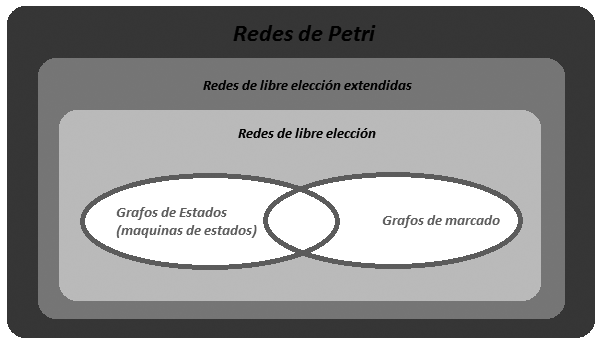
\includegraphics[width=1\linewidth]{./marco_teorico/redes_de_petri/img/Petri08}
		\caption{Subclases de Redes de Petri}
		\label{fig:Petri08}
	\end{figure}
	
	\subsection{Grafos o m�quinas de estado}

		Para representar una m�quina de estados con una Red de Petri, se deben cumplir las siguientes condiciones: 
		cada transici�n tiene un �nico arco de entrada y un �nico arco de salida, las plazas no tienen restricci�n 
		y solo existe un token en toda la red. Esto significa que no puede existir concurrencia, pero si puede 
		haber conflictos. Los conflictos se deben a que como una plaza puede tener muchos arcos de salida, no se 
		puede determinar hacia donde ir� un token. Por ejemplo, en la Figura \ref{fig:Petri09}un token 
		en la plaza $P0$ generar� conflicto entre las transiciones $T0$ y $T1$ dado que no se puede determinar cual 
		debe ser disparada.
		\begin{figure}[H]
			\centering
			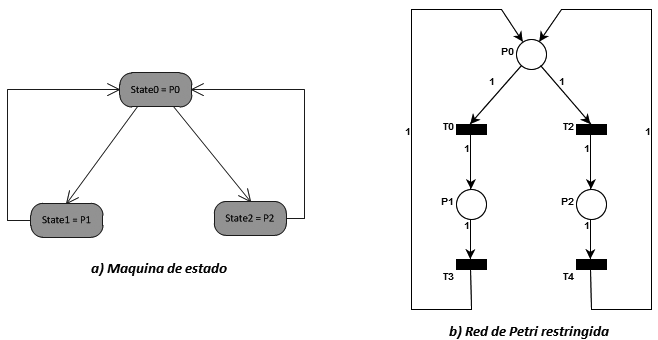
\includegraphics[width=.8\linewidth]{./marco_teorico/redes_de_petri/img/Petri09}
			\caption{Red de Petri restringida a m�quina de estados}
			\label{fig:Petri09}
		\end{figure}
		
		Matem�ticamente, sea $t$ una transici�n perteneciente al conjunto de transiciones $T$ se tiene que:
		\begin{equation}
			\forall t\in T : \mid t\bullet \mid =\mid\bullet t \mid =1
			\label{eq:petri_state_machine}
		\end{equation}
		
		\begin{figure}[H]
			\centering
			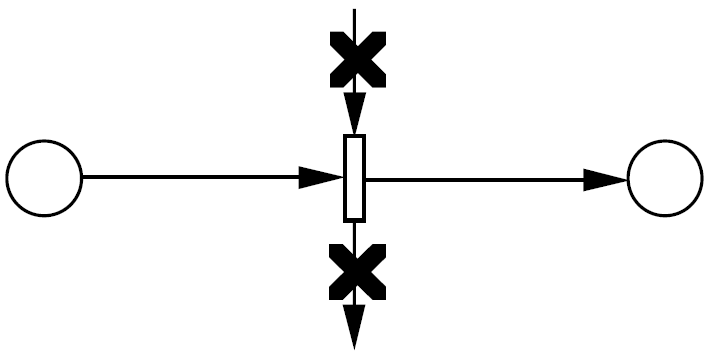
\includegraphics[width=0.25\linewidth]{./marco_teorico/redes_de_petri/img/Petri10}
			\caption{Ilustraci�n de la restricci�n para formar m�quinas de estados}
			\label{fig:Petri10}
		\end{figure}
		
		Generando un modelo con Redes de Petri que cumpla la restricci�n de la Ecuaci�n \ref{eq:petri_state_machine}
		es posible garantizar que el modelo cumple con todas las propiedades propias de las m�quinas de estado, 
		es decir, es conservativa y acotada. La propiedad de vivacidad en este tipo de redes, es simple de 
		demostrar y puede ser calculada de forma lineal con el algoritmo de Tarjan \cite{diaz_petri}.
	
	\subsection{Grafos de marcado}
	
		Para representar un grafo marcado con una Red de Petri debe cumplirse que: una plaza s�lo puede tener un 
		�nico arco de entrada y un �nico arco de salida, las transiciones no tienen restricciones. De esta manera, 
		si es posible que exista concurrencia y adem�s, no existen conflictos dado que un token solo puede 
		disparar una transici�n.
	 
		Matem�ticamente, sea $p$ una plaza perteneciente al conjunto de plazas $P$ se tiene que:
		\begin{equation}
			\forall p\in P : \mid p\bullet \mid =\mid\bullet p \mid =1
			\label{eq:petri_grafo_marcado}
		\end{equation}
		
		\begin{figure}[H]
			\centering
			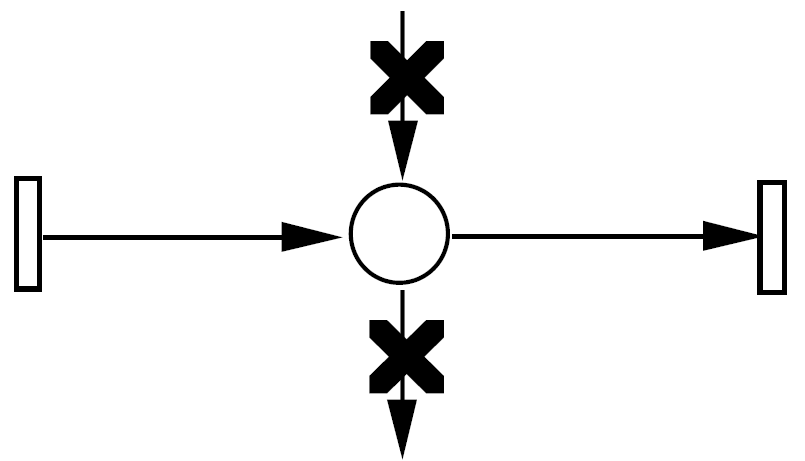
\includegraphics[width=0.25\linewidth]{./marco_teorico/redes_de_petri/img/Petri11}
			\caption{Ilustraci�n de la restricci�n para formar grafos de marcado.}
			\label{fig:Petri11}
		\end{figure}	
		
		Si la Red de Petri es de este tipo, la red es viva (sin deadlock) si y s�lo si cualquier circuito 
		elemental de la red incluye un lugar que inicialmente estaba marcado \cite{diaz_petri}.
		Una red de este tipo, ser� estructuralmente limitada si es fuertemente conectada \cite{diaz_petri}.
	
	\subsection{Redes de libre elecci�n}
		
		En las redes de libre elecci�n, todo arco que va desde una plaza hacia una transici�n, es el �nico arco 
		que sale desde esa plaza o es el �nico que entra en esa transici�n.
		\begin{equation}
			\forall p\in P : (\mid p\bullet \mid\leq 1) \vee (\mid\bullet(p\bullet) \mid =\{1\}
			\label{eq:petri_libre_eleccion}
		\end{equation}
		
		\begin{figure}[H]
			\centering
			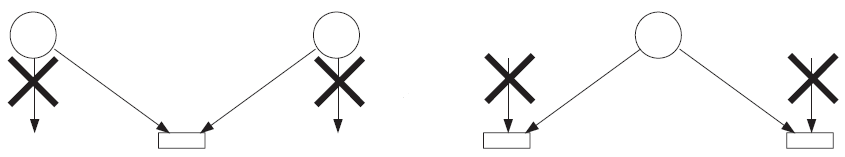
\includegraphics[width=0.7\linewidth]{./marco_teorico/redes_de_petri/img/Petri12}
			\caption{Red de elecci�n libre}
			\label{fig:Petri12}
		\end{figure}	
		
	\subsection{Redes de elecci�n libre extendidas}
	
		Si dos lugares tienen alguna transici�n de salida com�n, entonces ellos tienen todas sus transiciones de 
		salida en com�n, matem�ticamente es equivalente a:
		\begin{equation}
			Sea\;p1\;y\;p2\in P: p1\bullet \cap p2\bullet \neq \phi \Rightarrow \mid p1\bullet \mid=\mid p1\bullet
			\mid
			\label{eq:petri_libre_extendida}
		\end{equation}

		\begin{figure}[H]
			\begin{center}
			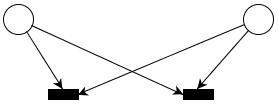
\includegraphics[width=0.3\linewidth]{./marco_teorico/redes_de_petri/img/Petri13}
				\end{center}
				\caption{Red de elecci�n libre extendida}
				\label{fig:Petri13}
		\end{figure}	
		
		De lo definido se puede notar que si una $t$ est� sensibilizada, todas las transiciones estar�n 
		estructuralmente en conflicto. Por lo que se puede elegir libremente entre varias transiciones para disparar.
	  
	
	% Extensiones de las Redes de Petri
		%%%%%%%%%%%%%%%%%%%%%%%%%%%%%%%%%%%%%%%%%%%%%%%%%%%%%%%%%%%%%%%%%%%%%%%%%%%%%%%%
%	TRABAJO: Proyecto Integrador
%		Titulo: 	Desarrollo de IP cores con procesamiento de Redes de Petri 	
%					Temporales para sistemas multicore en FPGA					
%		Autores:	Juli�n Nonino												%					Carlos Renzo Pisetta										%		Director:	Orlando Micolini											
%%%%%%%%%%%%%%%%%%%%%%%%%%%%%%%%%%%%%%%%%%%%%%%%%%%%%%%%%%%%%%%%%%%%%%%%%%%%%%%%

% Path im�genes: ./marco_teorico/redes_de_petri/img
% Nombre predeterminado im�genes: petrixx
%	xx es el numero de imagen

\section{Extensiones de las Redes de Petri}
	\label{sec:extensiones}

	Las Redes de Petri analizadas hasta el momento, pueden ser extendidas agregando arcos inhibidores para considerar la ausencia de tokens como condici�n de sensibilizaci�n de una transici�n (\textbf{\emph{Redes de Petri con Arcos Inhibidores}}), marcas de tiempo para determinar intervalos en los cuales una transici�n puede ser disparada (\textbf{\emph{Redes de Petri con Tiempo}}), o valores de duraci�n en las transiciones(\textbf{\emph{Redes de Petri Temporizadas}}), probabilidades de disparo de transiciones (\textbf{\emph{Redes de Petri Estoc�sticas}}) o cualquier combinaci�n entre ellas.
	
	En la Figura \ref{fig:Petri14}, extra�da del libro \cite{diaz_petri}, se observa la evoluci�n de estas extensiones. Se encuentran marcadas, aquellas que se analizar�n en este trabajo. Las \emph{Redes de Petri con Arcos Inhibidores} est�n incluidas dentro de �tem \emph{Place-transition Petri nets 1962, 1969}.
		
	\begin{figure}[H]
		\centering
		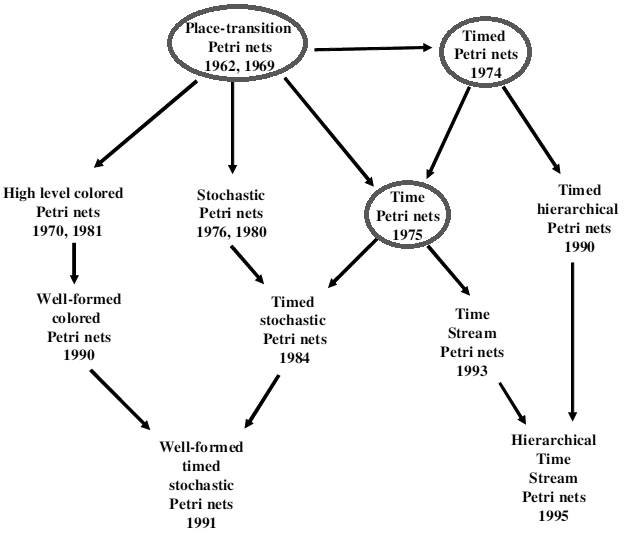
\includegraphics[width=1\linewidth]{./marco_teorico/redes_de_petri/img/Petri14}
		\caption{Extensiones de las Redes de Petri}
		\label{fig:Petri14}
	\end{figure}	
		
	
	% Redes de Petri con Arcos Inhibidores de peso unitario
		%%%%%%%%%%%%%%%%%%%%%%%%%%%%%%%%%%%%%%%%%%%%%%%%%%%%%%%%%%%%%%%%%%%%%%%%%%%%%%%%
%	TRABAJO: Proyecto Integrador
%		Titulo: 	Desarrollo de IP cores con procesamiento de Redes de Petri 	
%					Temporales para sistemas multicore en FPGA					
%		Autores:	Juli�n Nonino												%					Carlos Renzo Pisetta										%		Director:	Orlando Micolini											
%%%%%%%%%%%%%%%%%%%%%%%%%%%%%%%%%%%%%%%%%%%%%%%%%%%%%%%%%%%%%%%%%%%%%%%%%%%%%%%%

% Path im�genes: ./marco_teorico/redes_de_petri/img
% Nombre predeterminado im�genes: petrixx
%	xx es el numero de imagen

\section{Redes de Petri con Arcos Inhibidores de peso unitario}
	\label{sec:arcos_inhibidores}

	En las Redes de Petri vistas anteriormente las transiciones est�n sensibilizadas cuando en las plazas de entrada existe una cantidad igual o mayor de tokens que el peso del arco que los une. Pero, en algunas situaciones, ser�a necesario que una transici�n se encuentre sensibilizada cuando no existan tokens en alguna de sus plazas de entrada. Para este fin existen los arcos inhibidores. Los arcos inhibidores se representan con una l�nea finalizada en un c�rculo. Se debe destacar que s�lo pueden ir desde plazas hacia las transiciones, nunca al rev�s. 

	\subsection{Definici�n matem�tica}

	Una Red de Petri marcada con arcos inhibidores queda definida por una 6-tupla de la siguiente manera:
	\begin{equation*}
		PN={P,T,I^-,I^+,H,m_0}
	\end{equation*}
	
	El elemento nuevo es la matriz \emph{H} llamada \textbf{matriz de inhibici�n} que es una matriz de $p$ filas y $t$ columnas. Siendo $p$ la cantidad de plazas de la red y $t$ la cantidad de transiciones.
	
	Es una matriz binaria, sus elementos solo pueden valer cero (0) o uno (1). Un \emph{uno} en la posici�n $a_{ij}$ indica que la plaza $i$ esta unida a la transici�n $j$ a trav�s de un arco inhibidor. 
	
	\subsection{Transiciones sensibilizadas en Redes de Petri con Arcos Inhibidores}
	
		Se pondr� como ejemplo la siguiente Red de Petri.
		\begin{figure}[H]
			\centering
			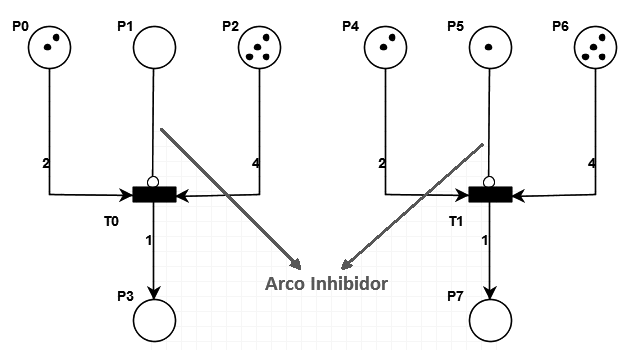
\includegraphics[width=.6\linewidth]{./marco_teorico/redes_de_petri/img/Petri15}
			\caption{ Ejemplo Red de Petri con Arco Inhibidor}
			\label{fig:Petri15}
		\end{figure}	
		
		En la Figura \ref{fig:Petri15}, se ve la representaci�n de un arco inhibidor y c�mo afecta a la transici�n. En la red de la izquierda, la transici�n $T0$ se encuentra sensibilizada mientras que en la red de la derecha la transici�n $T1$ no lo est�, por lo tanto no es posible que se dispare.
	
		Ahora, en una \textbf{\emph{Red de Petri con Arcos Inhibidores}}, se dice que una transici�n esta sensibilizada cuando se cumplen las siguientes condiciones:
		\begin{enumerate}
  			\item $\forall p_i \in I^-(t_j) : m(p_i) \geq W_{ij}$
  				\\
  				Siendo $W_{ij}$ el peso del arco (no inhibidor) que une la plaza $i$ con la transici�n $j$.
			\item Todas las plazas unidas a $t_j$ con arcos inhibidores no deben tener tokens.	
		\end{enumerate}
		
	\subsection{Ejecuci�n de una Red de Petri con Arcos Inhibidores}
			
		La ecuaci�n de estado para una Red de Petri con aros inhibidores toma la siguiente forma:
		\begin{equation}
			m_{i+1} = m_i  + I� \left[ \delta\;and\;f_H (m_i,\delta) \right]
			\label{eq:estado_petri_arcos_inhibidores}
		\end{equation}

		Como se ve, se agrega una funci�n $f$ que depende del marcado actual, del disparo a realizar y, de una funci�n $H$ que determina si una transici�n est� sensibilizada o no de acuerdo a  los arcos inhibidores. Esta funci�n toma solo valores ceros y unos, y al estar en una operaci�n $and$ con el disparo, puede inhibirlo y hacer que no produzca efectos.
		
		A continuaci�n se detalla la funci�n $f$.
		\begin{equation}
			f_H(m_i,\delta) = M_{=0}(m_i)\; nand \;(H � \delta)
			\label{eq:fun_inhibicion}
		\end{equation}
			
		La funci�n $M_{=0}()$ es una funci�n vectorial de $p$ elementos. Donde $p$ es la cantidad de plazas. Cada componente $k$ del resultado de la funci�n $M_{=0}()$ toma su valor de la siguiente ecuaci�n:
		\begin{equation}
			M_{=0}(m)_k =
				\begin{cases} 
					0 & \text{si } m_{ij} \neq 0
					\\
					1 & \text{si } m_{ij}= 0				
				\end{cases}		
			\label{eq:funcion_igual_cero}
		\end{equation}

	
	% Redes de Petri Temporales
		%%%%%%%%%%%%%%%%%%%%%%%%%%%%%%%%%%%%%%%%%%%%%%%%%%%%%%%%%%%%%%%%%%%%%%%%%%%%%%%%
%	TRABAJO: Proyecto Integrador
%		Titulo: 	Desarrollo de IP cores con procesamiento de Redes de Petri 	
%					Temporales para sistemas multicore en FPGA					
%		Autores:	Juli�n Nonino												%					Carlos Renzo Pisetta										%		Director:	Orlando Micolini											
%%%%%%%%%%%%%%%%%%%%%%%%%%%%%%%%%%%%%%%%%%%%%%%%%%%%%%%%%%%%%%%%%%%%%%%%%%%%%%%%

% Path im�genes: ./marco_teorico/redes_de_petri/img
% Nombre predeterminado im�genes: petrixx
%	xx es el numero de imagen

\section{Redes de Petri Temporales}
	\label{sec:redes_temporales}
	
	En los modelos de Redes de Petri descriptos hasta el momento, el tiempo no estaba considerado. 
	
	En el formalismo de Redes de Petri b�sico, o aut�nomo, la abstracci�n del entorno en el que la red evoluciona, incluyendo el tiempo como parte de este entorno, es total. Por lo que existe cierto indeterminismo en cuanto al tiempo: no se especifica cu�ndo se disparar� una transici�n que est� sensibilizada (ni si se disparar� realmente), tampoco cu�l de entre un grupo de transiciones en conflicto ser� la disparada \cite{garcia_izquierdo}.
	
	\newpage
	
	Las distintas interpretaciones con tiempo de las Redes de Petri han tratado de reducir el indeterminismo de distintas maneras. Entre estas interpretaciones est�n:
	\begin{enumerate}
	  	\renewcommand{\theenumi}{\Alph{enumi}}
	  	\item \underline{Redes de Petri Estoc�sticas (Stochastic Petri Net)}
	  		\\
			Se introduce una estimaci�n estoc�stica respecto del instante de disparo de una transici�n.
		\item \underline{Redes de Petri Temporizadas (Timed Petri Net)}
			\\
			Introduce una condici�n de tiempo que establece la duraci�n de la transici�n.
		\item \underline{Redes de Petri con Tiempo (Time Petri Net)}
			\\
			Introducen cotas temporales entre las cuales la transici�n puede o debe ser disparada.
	\end{enumerate}
	
	\begin{figure}[H]
		\centering
		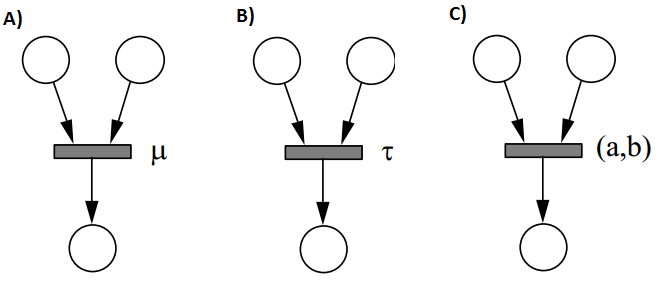
\includegraphics[width=0.9\linewidth]{./marco_teorico/redes_de_petri/img/Petri16}
		\caption{Interpretaciones de Redes de Petri Temporales}
		\label{fig:Petri16}
	\end{figure}
	
	Existen dos maneras de interpretar el par�metro temporal asociado a una transici�n:
	\begin{itemize}
		\item Cuando el par�metro temporal determina el tiempo que ha de transcurrir desde que una transici�n queda sensibilizada hasta que se dispara, procedi�ndose entonces a la retirada y colocaci�n de marcas de forma at�mica, se habla de \textbf{\emph{tiempo de sensibilizaci�n (enabling time)}}. Est� relacionada con las \textbf{\emph{Redes de Petri con Tiempo}} (Red C de la Figura \ref{fig:Petri16}).
		\item El par�metro temporal puede determinar tambi�n el tiempo que debe transcurrir entre la retirada (instant�nea) de marcas de los lugares de entrada, y la colocaci�n (instant�nea) de marcas en los lugares de salida; en �ste caso se habla de tiempo de \textbf{\emph{disparo (firing time)}}. Esto es, el disparo de la transici�n tiene tres fases (retirada de marcas de entrada, disparo, colocaci�n de marcas de salida) y no es at�mico, sino que tienen una duraci�n. Por ello esta interpretaci�n es tambi�n conocida como sem�ntica de duraci�n. Est�n asociadas con las \textbf{\emph{Redes de Petri Temporizadas}} (Red B de la Figura \ref{fig:Petri16}).
	\end{itemize}
	
	Este cap�tulo se centrar� en:
	\begin{itemize}
		\item \textbf{\emph{Redes de Petri con Tiempo:}}
			\\
			En estas redes, cada transici�n tiene asociado un intervalo $[a , b]$ que abarca todas las posibilidades de duraci�n de la actividad que la transici�n modela.
		\item \textbf{\emph{Redes de Petri Temporizadas:}}
			\\
			En estas redes, cada transici�n tiene asociado un par�metro $[a]$ que establece la duraci�n de la transici�n, es decir la duraci�n del intervalo entre que se extraen los tokens de las plazas de entrada y se colocan los tokens en las plazas de salida.
	\end{itemize}
		
	\subsection{Redes de Petri con Tiempo}
		\label{subsec:redes_con_tiempo}
		
		En �sta secci�n se describir�n las \textbf{\emph{Redes de Petri con Tiempo}} como la red \emph{C} de la Figura \ref{fig:Petri16}).
		
		\subsubsection{Definici�n matem�tica}
			Una \emph{Red de Petri Marcada con Tiempo}, se define matem�ticamente como una 7-tupla de la siguiente manera:
			\begin{equation*}
				PN = \{P, T, I^-, I^+, H, m_0, IS\}
			\end{equation*}
			D�nde,
			\begin{itemize}
				\item \textbf{P} es un conjunto finito y no vac�o de plazas.
				\item \textbf{T} es un conjunto finito y no vac�o de transiciones.
				\item \textbf{$I^+$} e \textbf{$I^-$} son las matrices de incidencia positiva y negativa respectivamente.
					\begin{equation*}
						P�T\rightarrow \mathbb{Z}
					\end{equation*}
				\item H es la matriz de arcos inhibidores.
					\begin{equation*}
						P�T\rightarrow\{0,1\}
					\end{equation*}
				\item $m_0$ es el marcado inicial de la red.
					\begin{equation*}
						P\rightarrow \mathbb{N}
					\end{equation*}
				\item IS es el conjunto de intervalos est�ticos asociados a cada transici�n.
					\begin{equation*}
						T\rightarrow \mathbb{Q}^+ � (\mathbb{Q}^+ \cup \infty)
					\end{equation*}
			\end{itemize}
			
			La funci�n \textbf{\emph{IS}} asocia a cada transici�n un par de valores que representan los l�mites temporales m�ximo y m�nimo entre los cuales la transici�n podr� ser disparada. De manera tal que $IS(t) = [min,max]$. Donde $t$ es una transici�n perteneciente a $T$. Como la funci�n $IS$ representa un intervalo temporal se deben cumplir las siguientes condiciones:
			\begin{itemize}
				\item $0 	\leq 	min	\langle	\inf$
				\item $0 	\leq 	max	\leq 	\inf$
				\item $min	\leq 	max \text{ si } max \neq \infty$
				\item $min	\langle max \text{ si } max   =	 \infty$
			\end{itemize}
			Al valor $min$ se le suele llamar \textbf{Earliest Firing Time EFT (Instante de disparo m�s temprano)}. Y, al valor $max$ se le llama \textbf{Latest Firing Time LFT (Instante de disparo m�s tard�o)}.
				
			Existen dos tipos de intervalos destacables:
			\begin{itemize}
				\item \emph{Intervalo puntual}
					\begin{equation*}
						[\alpha,\alpha]
					\end{equation*}
					En este caso, el tiempo de sensibilizaci�n es fijo, luego de que transcurra el tiempo $\alpha$ la transici�n debe dispararse. Un disparo inmediato es representado por $\alpha=0$ y se comporta como en las Redes de Petri vistas anteriormente.
			\item \emph{Intervalo sin restricci�n temporal}\\
				\begin{equation*}
					[0,\infty]			
				\end{equation*}
				La transici�n no tiene restricciones temporales para dispararse, se disparar� en alg�n momento despu�s de sensibilizarse.
			\end{itemize}
			
		\subsubsection{Regla de disparo de transiciones}
			
			El intervalo de tiempo definido $(min, max)$ indica el tiempo \emph{m�nimo} que debe transcurrir luego del momento en el que se sensibiliza la transici�n y el tiempo \emph{m�ximo} para que pueda ser disparada, luego de esto, la transici�n no podr� ser disparada.
			
			Suponiendo que la transici�n $t_i$ comienza a estar sensibilizada en el instante $w_i$, que contin�a sensibilizada y que su intervalo asociado es $(min_i, max_i)$, el disparo de la transici�n se producir� no antes del instante $w_i + min_i$, y no mas tarde del instante $w_i + max_i$. El intervalo de tiempos de disparo v�lidos para $ti$ ser�, por tanto $[w_i + min_i, w_i + max_i]$.
		
		\subsubsection{Estados en una Red de Petri con Tiempo}
			
			En estas Redes de Petri, el estado de la red queda definido por el vector de marcado $m$ de la misma y por un vector $Intervalo$ que lleva la marca de tiempo de cada transici�n. Por lo tanto el estado de una Red de Petri con Tiempo queda definido por:
			\begin{equation*}
				E = (m_0,Intervalo)
				\label{eq:estado_con_time}
			\end{equation*}
			
			Ahora, al disparar una transici�n $t$ en un instante $w_j$ produce un cambio desde el estado $E = (m,Intervalo)$ a un nuevo estado $E' = (m',Intervalo')$. El nuevo marcado $m'$ se determina con la ecuaci�n de estado vista anteriormente. Por otro lado, la actualizaci�n del intervalo para cada transici�n $k$ sigue las siguientes reglas:
			\begin{itemize}
				\item $Intervalo'(k) = \infty$ si la transici�n $k$ no est� sensibilizada.
				\item $Intervalo'(k) = Intervalo(k) + 1$ si $k\neq t$, en el marcado $m$ esta sensibilizada y sigue est�ndolo en el marcado $m'$. 
				\item $Intervalo'(k) = 0$ si $k = t$ o $k$ comienza a estar sensibilizada en el marcado $m'$.
			\end{itemize}
	
	\subsection{Redes de Petri Temporizadas}
		\label{subsec:redes_temporizadas}
		
		En �sta secci�n se describir�n las \textbf{\emph{Redes de Petri Temporizadas}} como la red \emph{B} de la Figura \ref{fig:Petri16}).
		
		\subsubsection{Definici�n matem�tica}
		
			Una \emph{Red de Petri Marcada Temporizada}, se define matem�ticamente como una 7-tupla de la siguiente manera:  
			\begin{equation*}
				PN = \{P, T, I^-, I^+, H, m_0, Timer\}
			\end{equation*}
			D�nde,
			\begin{itemize}
				\item \textbf{P} es un conjunto finito y no vac�o de plazas.
				\item \textbf{T} es un conjunto finito y no vac�o de transiciones.
				\item \textbf{$I^+$} e \textbf{$I^-$} son las matrices de incidencia positiva y negativa respectivamente.
					\begin{equation*}
						P�T\rightarrow \mathbb{Z}
					\end{equation*}
				\item H es la matriz de arcos inhibidores.
					\begin{equation*}
						P�T\rightarrow\{0,1\}
					\end{equation*}
				\item $m_0$ es el marcado inicial de la red.
					\begin{equation*}
						P\rightarrow \mathbb{N}
					\end{equation*}
				\item es el conjunto de valores de duraci�n asociados a cada transici�n.
					\begin{equation*}
						T\rightarrow \mathbb{Q}^+
					\end{equation*}
			\end{itemize}
		
		El conjunto de valores \textbf{\emph{Timer}} asocia un valor racional \emph{duraci�n} a cada transici�n. De manera tal que $Timer(t)=duracion$. Donde $t$ es una transici�n perteneciente a $T$.
		
		Dado que duraci�n es una referencia de tiempo, se debe cumplir que $0 \leq duracion \langle \infty$.
		
		\subsubsection{Regla de disparos y estados en una Red de Petri Temporizada} 
		
			En una \emph{Red de Petri Temporizada}, el disparo de una transici�n implica tres etapas.
			\begin{enumerate}
				\item Al momento que se sensibiliza la transici�n, se extrae la cantidad de tokens de las plazas de entrada indicada por el arco que los une a dicha transici�n. Adem�s, se marca la transici�n como no sensibilizada.
					\begin{equation*}
						m_{i+1} = m_i +I^- � d
					\end{equation*}
				Se genera un nuevo estado provisorio formado a partir la extracci�n de los tokens que sensibilizaban la transici�n que se esta disparando. Tambi�n, en ese instante se comienza la cuenta de tiempo.
				\item Se espera el tiempo indicado por el valor de duraci�n de la transici�n. Con la transici�n marcada como no sensibilizada, se espera hasta que la cuenta de tiempo, que comenz� al extraerse los tokens, llegue al valor indicado por $Timer(d)$.
				\item Transcurrido el tiempo indicado por el valor de duraci�n asociado a la transici�n se colocan los tokens en las plazas de salida seg�n como indican los arcos que unen a las transiciones con dichas plazas.
					\begin{equation*}
						m_{i+2} = m_{i+1} +I^+ � d
					\end{equation*}
			\end{enumerate}


 				% Concurrencia y sincronizacion
 					%%%%%%%%%%%%%%%%%%%%%%%%%%%%%%%%%%%%%%%%%%%%%%%%%%%%%%%%%%%%%%%%%%%%%%%%%%%%%%%%
%	TRABAJO: Proyecto Integrador
%		Titulo: 	Desarrollo de IP cores con procesamiento de Redes de Petri 	
%					Temporales para sistemas multicore en FPGA					
%		Autores:	Juli�n Nonino												%					Carlos Renzo Pisetta										%		Director:	Orlando Micolini											
%%%%%%%%%%%%%%%%%%%%%%%%%%%%%%%%%%%%%%%%%%%%%%%%%%%%%%%%%%%%%%%%%%%%%%%%%%%%%%%%

% Path im�genes: ./marco_teorico/concurrencia/img
% Nombre predeterminado im�genes: concurrenciaxx
%	xx es el numero de imagen

\chapter{Concurrencia y Sincronizaci�n}
	\label{chap:chap_concurrencia}

	En los sistemas de computaci�n actuales conviven m�ltiples procesos que cooperan para lograr determinados objetivos y compiten por recursos del sistema, entre ellos el procesador, la memoria RAM, los puertos de entrada/salida, etc.
	
	Dado que generalmente el n�mero de procesos en un sistema supera ampliamente el n�mero de recursos, se deben establecer formas de comunicaci�n y sincronizaci�n entre ellos que hagan que el sistema funcione correctamente.

	En �ste capitulo se definir� cuando dos programas son concurrentes y/o paralelos y las condiciones que deben cumplirse para que dos secciones de c�digo fuente puedan ser ejecutadas de manera concurrente. Luego, se ver� que la ejecuci�n concurrente de procesos trae aparejados ciertos problemas como el interbloqueo y la inanici�n. Por esta raz�n deben utilizarse ciertos mecanismos de control para garantizar la correcta ejecuci�n de los programas, entre ellos, los sem�foros y los monitores.

	El objetivo de este cap�tulo es que el lector adquiera una idea general sobre la programaci�n concurrente y sobre los problemas inherentes a la misma.
	
	% Concurrencia
		%%%%%%%%%%%%%%%%%%%%%%%%%%%%%%%%%%%%%%%%%%%%%%%%%%%%%%%%%%%%%%%%%%%%%%%%%%%%%%%%%%%%%
%																					%
%	TRABAJO: Proyecto Integrador													%
%																					%
%		Titulo: 	Desarrollo de IP cores con procesamiento de Redes de Petri 		%
%					Temporales para sistemas multicore en FPGA						%
%																					%
%		Autores:	Juli�n Nonino													%
%					Carlos Renzo Pisetta											%
%		Director:	Orlando Micolini												%
%																					%
%	Parte: Marco Teorico															%
%	Capitulo: FPGA - IP cores - HDL													%
%	Seccion: Concurrencia y Paralelismo												%	
%	Archivo: concurrencia.tex														%
%																					%
%%%%%%%%%%%%%%%%%%%%%%%%%%%%%%%%%%%%%%%%%%%%%%%%%%%%%%%%%%%%%%%%%%%%%%%%%%%%%%%%%%%%%

% Path Imagenes: ./marco_teorico/concurrencia/img
% Nombre predeterminado imagenes: concurrenciaxx
%	xx es el numero de imagen

\section{Concurrencia y Paralelismo}
	\label{sec:concurrencia}

	Dos procesos ser�n concurrentes cuando la primera instrucci�n de uno de ellos se 
	ejecuta despu�s de la primera instrucci�n de otro proceso y antes de la �ltima. \cite{palma}
	
	No es necesario que se ejecuten al mismo tiempo, alcanza con el hecho de que se intercalen 
	sus instrucciones. En caso de ejecutarse al mismo tiempo se dice que hay programaci�n paralela.
	
	La programaci�n concurrente es un paralelismo potencial dependiente del hardware que lo soporte.
	
	\subsection{Condiciones de Bernstein}
		\label{subsec:condiciones_bernstein}
		
		No todas las partes de un programa pueden ejecutarse concurrentemente. Las condiciones de 
		Bernstein permiten determinar formalmente que partes de un programa pueden ejecutarse 
		concurrentemente y cuales no.
		\\ 
		
		Sean el conjunto de instrucciones $S_k$, pueden determinarse dos subconjuntos a partir de �l.
		\begin{itemize}
		  	\item $L(S_k) = \{a_1, a_2, \cdots, a_n\}$
		  		\\
				Subconjunto de $S_k$ que agrupa aquellas instrucciones que realizan lecturas de variables 
				durante la ejecuci�n del programa.
			\item $E(S_k) = \{b_1, b_2, \cdots , b_m\}$
				\\
				Subconjunto de $S_k$ que agrupa aquellas instrucciones que realizan escrituras de variables 
				durante la ejecuci�n del programa.
		\end{itemize}
		Luego, para que dos conjuntos de instrucciones $S_i$ y $S_j$ puedan ser ejecutadas de manera concurrente
		se deben cumplir las siguientes condiciones.
		\begin{equation*}
			\begin{array}{c}
				% Primera Fila
					L(S_i) \bigcap E(S_i) = \emptyset
				\\
				
				\\
				% Segunda Fila
					E(S_i) \bigcap L(S_i) = \emptyset
				\\
				
				\\
				% Tercera Fila
					E(S_i) \bigcap E(S_i) = \emptyset
			\end{array}
		\end{equation*}

	\subsection{Problemas inherentes a la programaci�n concurrente}
	
		La intercalaci�n de instrucciones de diferentes procesos, debe ser bien manejada y controlada 
		dado que puede producir mal funcionamiento del sistema. Los problemas inherentes a la 
		concurrencia son:
		\begin{itemize}
		  	\item \emph{Exclusi�n mutua}: Se debe garantizar que si un proceso adquiere el recurso los 
		  		dem�s deber�n esperar hasta que sea liberado.
		  	\item \emph{Condici�n de sincronizaci�n}: hay situaciones en las que un proceso debe esperar 
		  		que ocurra alg�n determinado evento para poder continuar. Por ello se debe garantizar que 
		  		si el evento NO ocurri�, el proceso NO contin�e.
		  	\item \emph{Interbloqueo}: Esta situaci�n se produce cuando todos los procesos est�n esperando 
		  		un evento que nunca ocurrir�. Se debe garantizar que estas situaciones no ocurran.
		  	\item \emph{Interbloqueo activo}: se produce cuando un sistema ejecuta una serie de instrucciones 
		  		sin hacer ning�n progreso.
		  	\item \emph{Inanici�n}: en este caso, el sistema en su conjunto hace progresos, pero existe un 
		  		grupo de procesos que nunca progresaran pues no se les otorga tiempo de procesador para hacerlo.
		\end{itemize}
				
	\subsection{Exclusi�n mutua}

		La \emph{exclusi�n mutua} implica que dos o m�s procesos intentan acceder a un �nico recurso o variable 
		compartida entre ellos pero solo uno puede acceder a cada instante.
		
		Cuando se da un caso de estas caracter�sticas, se desea que todo lo que necesite hacer uno de los procesos 
		sobre el recurso se realice de manera indivisible y luego lo deje disponible para que otro proceso ejecute 
		sus instrucciones sobre el recurso. La idea ser�a que instrucciones de diferentes procesos que act�en sobre 
		un mismo recurso NO sean intercaladas en la ejecuci�n.

		A la porci�n de c�digo que se desea que se ejecute de manera indivisible o at�mica se le llama \emph{secci�n 
		cr�tica}. Se debe lograr que todas las instrucciones dentro de la secci�n critica se ejecuten en exclusi�n 
		mutua lo que implica que el hecho de que cuando uno de los procesos este ejecutando esa porci�n de c�digo 
		el resto no podr� hacerlo.
		
		\textbf{\emph{SOLO UNO de los procesos podr� estar en la secci�n cr�tica en un instante dado.}}
		
		\begin{figure}[H]
			\centering
			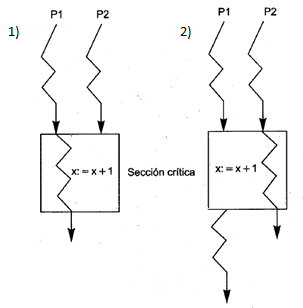
\includegraphics[width=0.6\linewidth,keepaspectratio]{./marco_teorico/concurrencia/img/concurrencia01}
			\caption{Secci�n cr�tica}
			\label{fig:concurrencia01}
		\end{figure}
		
		En la Figura \ref{fig:concurrencia01} se observa como dos procesos \emph{P1} y \emph{P2} intentan ejecutar 
		una porci�n de c�digo de una secci�n cr�tica. La imagen de la izquierda (1) muestra que el proceso \emph{P1} 
		consigue ingresar a ejecutar la secci�n critica. La imagen de la derecha (2) muestra que el proceso \emph{P2} 
		puede ingresar solo cuando el proceso \emph{P1} ya no esta en la misma.
		\\
		
		La exclusi�n mutua puede representarse con una Red de Petri de la siguiente manera.
		\begin{figure}[H]
			\centering
			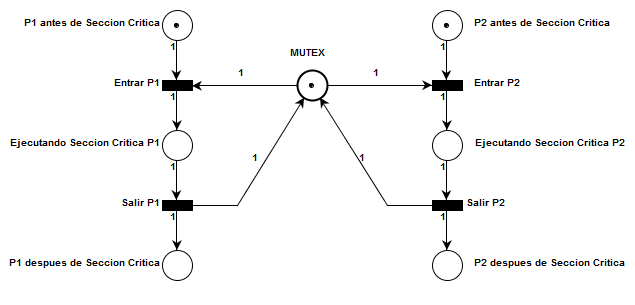
\includegraphics[width=1\linewidth,keepaspectratio]{./marco_teorico/concurrencia/img/concurrencia02}
			\caption{Exclusi�n mutua modelada con una Red de Petri}
			\label{fig:concurrencia02}
		\end{figure}
		En la Red de Petri de la Figura \ref{fig:concurrencia02} se representa una situaci�n de exclusi�n mutua. 
		La plaza \emph{MUTEX} esta limitada a un �nico token y el an�lisis de invariantes de plazas demuestra 
		formalmente la propiedad de exclusi�n mutua entre los procesos \emph{P1} y \emph{P2}.
		\begin{equation*}
			m(EjecutandoSCP1) + m(MUTEX) + m(EjecutandoSCP2) = 1
		\end{equation*}
		
	\subsection{Condici�n de sincronizaci�n}
	
		Existen situaciones en las que un recurso compartido por varios procesos se encuentra en un estado en el 
		que un proceso no puede hacer una determinada acci�n con el hasta que no cambie el estado. A esto se llama 
		\emph{condici�n de sincronizaci�n}.
		
		Por ello se debe contar con mecanismos que permitan bloquear a un proceso que no pueda hacer algo en un 
		momento determinado a la espera de alg�n evento. Pero tambi�n, mecanismos que permitan desbloquearlo 
		cuando el evento haya ocurrido.
		
	\subsection{Propiedades de los programas concurrentes}
		
		Para que un programa sea correcto debe cumplir las especificaciones funcionales. En el caso de los programas 
		concurrentes deben, adem�s, cumplir con una serie de propiedades inherentes a la concurrencia.
		Estas propiedades se agrupan en:
		\begin{itemize}
		  	\item \emph{Propiedades de seguridad}: aseguran que nada malo va a pasar durante la ejecuci�n del programa.
		  	\item \emph{Propiedades de vivacidad}: aseguran que algo bueno pasara eventualmente durante la ejecuci�n.
		\end{itemize}
	
		\subsubsection{Propiedades de seguridad}
			
			\begin{itemize}
			  	\item \emph{Exclusi�n mutua}: dado que existen recursos en el sistema que deben ser accedidos en exclusi�n 
			  		mutua, se debe garantizar que si un proceso adquiere el recurso los dem�s deber�n esperar hasta que sea 
			  		liberado.
			  	\item \emph{Condici�n de sincronizaci�n}: en las situaciones en las que un proceso debe esperar que ocurra 
			  		alg�n determinado evento para poder continuar, se debe garantizar que si el evento NO ocurri�, el proceso 
			  		NO contin�e.
			  	\item \emph{Interbloqueo}: Esta situaci�n se produce cuando todos los procesos est�n esperando un evento que 
			  		nunca ocurrir�. Se debe garantizar que estas situaciones no ocurran. Tambi�n se conoce con el nombre de 
			  		\textbf{\emph{deadlock}}.
			\end{itemize}
		
		\subsubsection{Propiedades de vivacidad}
			
			\begin{itemize}
			  	\item \emph{Interbloqueo activo}: se produce cuando un sistema ejecuta una serie de instrucciones sin hacer 
			  		ning�n progreso. Se conoce como \textbf{\emph{livelock}}.
			  	\item \emph{Inanici�n}: en este caso, el sistema en su conjunto hace progresos, pero existe un grupo de 
			  		procesos que nunca progresaran pues no se les otorga tiempo de procesador para hacerlo. Tambi�n se 
			  		conoce como \textbf{\emph{starvation}}. 
			\end{itemize}
	
		\subsubsection{Ejemplo}
		
			El siguiente ejemplo ha sido extra�do de \cite{palma} e ilustra todos los problemas antes mencionados.
			\\
			
			Sea un juego donde hay dos equipos, el \emph{A} y el \emph{B}, y un juez con un pa�uelo.
			Cada jugador de un equipo tiene un n�mero del \emph{1} al \emph{3}. No puede haber jugadores del mismo 
			equipo con el mismo n�mero.
			
			El juez dice un n�mero y los dos rivales con el mismo n�mero van corriendo a buscar el pa�uelo. El que 
			lo agarre debe volver a su lugar sin que su rival le toque la espalda.

			A continuaci�n se describir�n, para �ste ejemplo, las propiedades mencionadas anteriormente.
			\begin{itemize}
			  	\item \emph{Exclusi�n mutua}: al pa�uelo puede agarrarlo solo un jugador a la vez, si lo agarran dos 
			  		puede romperse, lo que implicar�a un mal funcionamiento del sistema.
				\item \emph{Condici�n de sincronizaci�n}: un jugador debe esperar a que digan su n�mero para correr.
				\item \emph{Interbloqueo}: si un jugador se guarda el pa�uelo y se va. El juez esperar�a que se lo 
					devuelvan y los jugadores que el juez diga su nombre, pero ninguno de los eventos ocurrir�.
				\item \emph{Interbloqueo activo}: se producir�a si dos jugadores amenazan una y otra vez con agarrar 
					el pa�uelo pero ninguno lo hace.
				\item \emph{Inanici�n}: Podr�a pasar si el juez nunca dice el nombre de un jugador en particular.
			\end{itemize}
	
	\subsection{Interbloqueo}
		
		En un sistema donde los procesos compiten por limitados recursos, pueden producirse demandas contradictorias 
		de los mismos. Por ejemplo, si existen dos procesos, \emph{A} y \emph{B}, y dos recursos, \emph{R1} y \emph{R2}, 
		y ambos procesos necesitan los dos recursos para proseguir, si el proceso \emph{A} toma el recurso \emph{R1} y 
		el \emph{B} el recurso \emph{R2}, ambos procesos se bloquearan a la espera del otro recurso, pero ninguno liberara 
		el recuro que posee hasta no conseguir los dos. A esta situaci�n se la conoce como interbloqueo. \cite{stallings}
		
		\subsubsection{Condiciones para producir interbloqueo}
		
			El interbloqueo podr� producirse si se cumplen tres condiciones:
			\begin{enumerate}
			  	\item \emph{Exclusi�n mutua}: s�lo un proceso puede utilizar el recurso en un momento determinado.
			  	\item \emph{Retenci�n y espera}: un proceso puede mantener el recurso que se le asigno mientras espera 
			  		conseguir otro.
			  	\item \emph{No apropiaci�n}: ning�n proceso podr� ser forzado a abandonar un recurso que retiene.
			  	\item \emph{Circulo viciosos de espera}: Existe una cadena cerrada de procesos donde cada proceso retiene 
			  		un recurso que necesita un proceso que le sigue en la cadena.
			\end{enumerate}

			Las tres primeras condiciones son necesarias pero no suficientes para que se produzca interbloqueo.
			
			La cuarta es una consecuencia potencial de las tres primeras y, en caso de darse, generar� un \textbf{\emph{c�rculo 
			vicioso de espera irresoluble}}.
			
			Un c�rculo de espera irresoluble es la definici�n de interbloqueo.
				
		\subsubsection{Prevenci�n del interbloqueo}
			
			La idea es intentar dise�ar un sistema donde, la posibilidad de interbloqueo este excluida.
			\newpage
			Existen dos tipos de m�todos para internar prevenir una situaci�n de interbloqueo:
			\begin{itemize}
			  	\item \emph{Indirectos:} intentan impedir la aparici�n de las tres condiciones necesarias (1,2 y 3).
			  	\item \emph{Directos}: intentan evitar la aparici�n de un c�rculo vicioso de espera irresoluble.
			\end{itemize}
		
			Existen diversas t�cnicas de prevenci�n de interbloqueo relacionadas a cada una de las condiciones que 
			pueden producirlo.
			\begin{itemize}
			  	\item \emph{Exclusi�n mutua}: En general no puede anularse, si un recurso necesita ser accedido en 
			  		exclusi�n mutua no podr� hacerse un acceso de sin esta condici�n.
			  	\item \emph{Retenci�n y espera}: esta condici�n puede prevenirse haciendo que todos los procesos 
			  		soliciten todos los recursos que necesitan al mismo tiempo y bloqueando al proceso hasta que 
			  		todos los recursos que necesite est�n disponibles simult�neamente. Pero esta soluci�n es 
			  		ineficiente por dos factores:
			  		\begin{itemize}
			  		  	\item Un proceso puede estar suspendido durante mucho tiempo esperando todos los recursos 
			  		  		cuando podr�a haber avanzado con algunos de ellos.
			  		  	\item Los recursos asignados a un proceso pueden permanecer mucho tiempo sin usarse. En ese 
			  		  		tiempo otro proceso podr�a haberlos utilizado.
			  		\end{itemize}
			  	\item \emph{No apropiaci�n}: puede prevenirse de varias maneras:
			  		\begin{itemize}
			  		  	\item Si un proceso que retiene muchos recursos pide uno m�s y se le niega el pedido, se le 
			  		  		obligara a liberar todos los recursos anteriores y volver a pedirlos cuando los necesite 
			  		  		junto con el recurso adicional.
			  		  	\item Si un proceso pide recursos retenidos por otro proceso, el sistema operativo puede 
			  		  		expulsar al segundo proceso y exigirle que libere sus recursos. Este sistema evitara 
			  		  		interbloqueo solo si existen dos procesos con la misma prioridad.
			  		\end{itemize}
			  	\item \emph{C�rculo vicioso de espera}: esta condici�n puede prevenirse definiendo un ordenamiento lineal 
			  		de los tipos de recursos. Por ejemplo si un proceso solicit� recursos del tipo \emph{R}, solo podr� 
			  		realizar peticiones posteriores sobre recursos siguientes a \emph{R} en el ordenamiento. Esta t�cnica 
			  		puede ser ineficiente porque se puede retardar procesos deneg�ndoles recursos innecesariamente. 
			\end{itemize}
			
		\subsubsection{Predicci�n del interbloqueo}
		
			En la prevenci�n del interbloqueo se obligaba a impedir que sucedieran algunas de las cuatro condiciones que 
			pueden llevar al interbloqueo. Pero con esto, se llega a un uso ineficiente de los recursos y a una ejecuci�n 
			ineficiente de los procesos.
			
			En cambio, en la predicci�n, se permiten alcanzar las tres condiciones necesarias pero se realizan elecciones 
			acertadas para evitar llegar al punto del interbloqueo. Por lo tanto, la predicci�n permite m�s concurrencia 
			que la prevenci�n.
			
			Con predicci�n de interbloqueo, antes de concederle un recurso a un proceso, se decidir� din�micamente si esa 
			petici�n puede llevar a interbloqueo en caso de concederse. Por lo tanto, la predicci�n exige saber las peticiones 
			futuras de recursos.

			Elementos de la predicci�n del interbloqueo son:
			\begin{itemize}
			  	\item \emph{Negativa de iniciaci�n de procesos}: no se iniciara un proceso si sus demandas pueden llevar a un 
			  		interbloqueo. Un nuevo proceso comenzara solo si puede satisfacerse la demanda m�xima de todos los procesos 
			  		actuales m�s la del nuevo proceso. Esta estrategia no es �ptima ya que asume el peor caso, que todos los 
			  		procesos expresen su mayor demanda al mismo tiempo.
			  	\item \emph{Negativa de asignaci�n de recursos}: no se conceder� una solicitud de incrementar los recursos de un 
			  	proceso si esta petici�n puede llevar a interbloqueo. Esta estrategia fue enunciada por Dijkstra y se conoce como 
			  	\textbf{\emph{algoritmo del banquero}}.
			\end{itemize}
			
		\subsubsection{Algoritmo del banquero}

			Este algoritmo comienza definiendo un estado seguro, donde existe al menos un orden en el cual todos los procesos 
			pueden ejecutar hasta el final sin producir interbloqueo. Un estado inseguro es, naturalmente, un estado no seguro.
			
			Cuando un proceso realiza un petici�n de recursos, se supone que se concede, se actualiza el estado del sistema, 
			si es seguro se concede la solicitud, en caso contrario se bloquea el proceso hasta que sea seguro conceder la 
			solicitud.
			
			El algoritmo es conocido de esta manera por analog�a con el problema de un banco cuando los clientes desean obtener 
			dinero prestado. Los clientes ser�an los procesos y el dinero los recursos. De esta manera, el banco tiene una 
			reserva limitada de dinero para prestar y un conjunto de clientes. Si un cliente pide un pr�stamo, el banquero 
			puede optar por rechazarlo si existe riesgo de que el banco se quede sin fondos suficientes para pr�stamos futuros.

			Como se observa, se debe conocer la m�xima solicitud por anticipado, los procesos deben ser independientes y el 
			n�mero de recursos y procesos debe ser fijo.
	

		
	% Sincronizaci�n
		%%%%%%%%%%%%%%%%%%%%%%%%%%%%%%%%%%%%%%%%%%%%%%%%%%%%%%%%%%%%%%%%%%%%%%%%%%%%%%%%
%	TRABAJO: Proyecto Integrador
%		Titulo: 	Desarrollo de IP cores con procesamiento de Redes de Petri 	
%					Temporales para sistemas multicore en FPGA					
%		Autores:	Juli�n Nonino												%					Carlos Renzo Pisetta										%		Director:	Orlando Micolini											
%%%%%%%%%%%%%%%%%%%%%%%%%%%%%%%%%%%%%%%%%%%%%%%%%%%%%%%%%%%%%%%%%%%%%%%%%%%%%%%%

% Path im�genes: ./marco_teorico/concurrencia/img
% Nombre predeterminado im�genes: concurrenciaxx
%	xx es el numero de imagen

\section{Sincronizaci�n}
	\label{sec:sincronizacion}

	Para solucionar los problemas inherentes a la programaci�n concurrente, se utiliza lo que se llama \emph{sincronizaci�n entre los procesos}.

	En general, se habla de sincronizaci�n cuando determinados fen�menos ocurren o deben ocurrir en un determinado orden o a la vez.

	Para la Ingenier�a en Computaci�n, la sincronizaci�n es representada por las se�ales que se env�an los procesos para colaborar entre ellos o para indicar el estado de recursos compartidos, para indicar que un evento o acci�n ocurri� o no y determinar si un proceso puede continuar o no, etc�tera.

	Se dice que un recurso esta sincronizado cuando debe encontrarse en un estado determinado para que un proceso pueda utilizarlo. En otras palabras, se puede definir a la condici�n de sincronizaci�n como a la propiedad requerida de que un proceso no realice ninguna acci�n o evento hasta que otro proceso realice una determinada acci�n o evento.
	
	Existen diversos mecanismos que se utilizan para sincronizar procesos, entre ellos, los m�s comunes son los \textbf{\emph{sem�foros}} y los \textbf{\emph{monitores}}.

	\subsection{Sem�foros}
	
		Los sem�foros son un sistema de se�ales simples utilizadas por los procesos para comunicarse entre ellos y lograr la sincronizaci�n requerida.

		En este m�todo se tiene una variable de sincronizaci�n, del tipo entero no negativo, que indica la cantidad de recursos disponibles. Sobre esta variable se realizan dos tipos de operaciones:
		\begin{itemize}
		  	\item \emph{wait}: decrementa el valor del sem�foro solo si este es mayor que cero. Este proceso indica que se utiliza uno de los recursos que controla el sem�foro. Si el valor del sem�foro al momento de ejecutar la operaci�n \emph{wait} es cero, indica que no hay recursos disponibles y el proceso debe bloquearse hasta que se libere alguno.  
		  	\item \emph{signal}: es la acci�n de liberar un recurso que estaba siendo usado por otro proceso en el sem�foro. En caso de haber alg�n proceso bloqueado en el sem�foro se lo despierta para que utilice el recurso. De no existir ning�n proceso, se incrementa el valor del sem�foro. 	
		\end{itemize}
		\begin{figure}[H]
			\centering
			
\includegraphics[width=1\linewidth,keepaspectratio]{./marco_teorico/concurrencia/img/concurrencia03}
			\caption{Operaciones \emph{wait} y \emph{signal} sobre un sem�foro \emph{s}}
			\label{fig:concurrencia03}
		\end{figure}
		
		Aunque los sem�foros son un mecanismo de gran potencia, se pueden enunciar los siguientes inconvenientes al usarlos.
		\begin{enumerate}
		  	\item Es un mecanismo de bajo nivel, no estructurado, que f�cilmente puede llevar a errores transitorios. La ejecuci�n de cada secci�n cr�tica debe comenzar con un \emph{wait} y terminar con un \emph{signal} sobre el mismo sem�foro. Si se omite una de estas operaciones o se realizan sobre sem�foros diferentes puede derivar en un mal funcionamiento del sistema, como por ejemplo, no garantizar exclusi�n mutua en las secciones cr�ticas.
		  	\item No se puede restringir el tipo de operaciones realizadas sobre los recursos.
		  	\item Cuando se usan sem�foros, el programador puede olvidar incluir en alguna secci�n cr�tica todas las sentencias necesarias para el control de los objetos compartidos.
		  	\item Tanto la exclusi�n mutua como la condici�n de sincronizaci�n se implementan de la misma manera. Esto hace dif�cil, al ver un \emph{wait} o un \emph{signal}, discernir acerca del prop�sito con el que fueron incluidas. Como la exclusi�n mutua y la condici�n de sincronizaci�n son conceptos distintos se desear�a que tengan notaciones diferentes.
		  	\item Los programas que utilizan sem�foros son muy dif�ciles de mantener dado que el c�digo de sincronizaci�n est� repartido entre los distintos procesos. Por lo tanto cada vez que se realiza una modificaci�n hay que revisar cada proceso.
		\end{enumerate}

	\subsection{Monitores}
		
		Como se dijo, los sem�foros, generalmente se encuentran dispersos en el c�digo, lo que lo hace m�s confuso y muchas veces es dif�cil notar cual es el recurso compartido y determinar si est� correctamente sincronizado. Por ello, se necesita un sistema que sea igual de vers�til que los sem�foros pero que permita efectuar un control m�s estructurado de la exclusi�n mutua. Una herramienta con estas caracter�sticas fue propuesta por \emph{C. A. R. Hoare} en 1975 y es llamada \textbf{\emph{monitor}}.

		Un \emph{monitor} es un mecanismo de abstracci�n de datos, lo que permite representar de forma abstracta un recurso compartido mediante variables que indican su estado. El acceso a esas variables solo es posible a trav�s de un conjunto de funciones/m�todos que el monitor exporta al exterior.
		
		Al usar monitores en la sincronizaci�n y en la exclusi�n mutua, existen dos clases de procesos:
		\begin{itemize}
		  	\item \emph{Procesos Pasivos}: son los que implementan los monitores y quedan a la espera que un proceso activo ejecute los m�todos exportados por el monitor.
		  	\item \emph{Procesos Activos}: son aquellos procesos que en un momento determinado pueden requerir utilizar el recurso controlado por el monitor para lo cual llaman a los m�todos que �ste exporta. 
		\end{itemize}

		Dado que las variables compartidas se encuentran dentro del monitor, los procesos activos solo pueden utilizarlas mediante los m�todos que el monitor exporta. Las ventajas de esto son dos:
		\begin{enumerate}
		  	\item Los programadores de los procesos activos no deben preocuparse de c�mo esta implementado el recurso compartido, es m�s, si se mantienen los nombres de los procedimientos exportados, esta implementaci�n puede cambiar sin necesidad de modificar a los procesos activos.
		  	\item El programador del monitor no se debe preocupar en c�mo y donde ser� utilizado el monitor, ya que una vez que se comprob� que el monitor funciona correctamente, seguir� funcionando de forma correcta en diferentes contextos.
		\end{enumerate}


		Un monitor se compone de los siguientes elementos:
		\begin{itemize}
		  	\item Un \emph{conjunto de variables} locales que pueden denominarse permanentes. Se utilizan para almacenar el estado interno del recurso que representa el monitor. Se denominan permanentes ya que permaneces sin modificarse entre dos llamadas consecutivas al monitor y solo pueden ser accedidas dentro del mismo.
		  	\item Un \emph{c�digo de inicializaci�n} que se ejecuta antes que la primera instrucci�n ejecutable del programa y su fin es inicializar las variables permanentes.
		  	\item Un \emph{conjunto de procedimientos internos} que manipulan las variables permanentes.
		  	\item Una \emph{declaraci�n de los procedimientos que son exportados} y pueden ser accedidos por los procesos activos externos.
		\end{itemize}
				
		\subsubsection{Exclusi�n mutua en monitores}
			
			El control de la exclusi�n mutua en un monitor se basa en la existencia de una cola asociada al mismo que se denominara \emph{cola del monitor}. La gesti�n de esta cola se realiza de la siguiente manera:
			\begin{enumerate}
			  	\item Cuando un proceso activo est� dentro del monitor (ejecutando alguno de los procedimientos del mismo) y aparece otro proceso activo que intenta ejecutar otro (o el mismo) procedimiento, el c�digo de acceso al monitor bloquea el proceso que realiza la llamada y lo inserta en la cola del monitor (con pol�tica FIFO). As�, se impide que dos procesos est�n al mismo tiempo dentro del monitor.
			  	\item Cuando un proceso activo abandona el monitor, este �ltimo selecciona el proceso que est� al frente de la cola del monitor y lo desbloquea para que comience a ejecutar las operaciones que le solicit� al monitor. Si la cola estaba vac�a, el monitor queda libre y cualquier proceso activo que llame alguno de sus procedimientos entrar� al monitor. 
			\end{enumerate}

			Esto asegura que las variables compartidas nunca son accedidas concurrentemente. Una cuesti�n importante es que la responsabilidad de bloquear un proceso es del monitor y no del proceso. 
			
			Al comparar este sistema con un sem�foro se ve que en el caso de los sem�foros son los propios procesos activos los que manejan las pol�ticas de acceso a variables compartidas.
			
		\subsubsection{Condici�n de sincronizaci�n en monitores}
		
			Para que un monitor pueda controlar condiciones de sincronizaci�n, se utilizan las llamadas variables de condici�n que se declaran dentro del monitor. Los valores de estas variables no son accesibles por el programador y representan colas FIFO. Estas variables permiten bloquear un proceso que no puede seguir su ejecuci�n dentro de monitor y desbloquearlos cuando la situaci�n que provoco el bloqueo ya no se est� presente. Para conseguir esto se necesitan dos operaciones sobre las variables de condici�n. Las operaciones \textbf{\emph{delay}} y \textbf{\emph{resume}}. La operaci�n \emph{delay(C)}, siendo \emph{C} una variable de condici�n, hace que el proceso se bloquee en la cola asociada a dicha variable. Hay que remarcar que el proceso no puede bloquearse directamente, antes de bloquearse al final de la cola de la condici�n debe liberar la exclusi�n mutua que retiene sobre el monitor. Si un proceso ha sido bloqueado con la operaci�n \emph{delay(C)} solo puede ser desbloqueado con la operaci�n \emph{resume(C)}. Esta �ltima operaci�n despierta al proceso que est� al frente de la cola de la condici�n y lo prepara para su ejecuci�n. Si la cola estaba vac�a se transforma en una operaci�n nula.

			Con lo dicho hasta este punto, se podr�a decir que si un proceso que se est� ejecutando dentro del monitor ejecuta una operaci�n \emph{resume(C)}, se desbloquear� un proceso de esa cola que continuar� con su ejecuci�n dentro del monitor tambi�n. Esto lleva a una situaci�n con dos procesos dentro del monitor, lo que violar�a la exclusi�n mutua. Para evitar esto, el proceso que ejecuta el \emph{resume} ceder� cort�smente la exclusi�n mutua al reci�n desbloqueado. Y espera en una cola diferente llamada \textbf{\emph{cola de cortes�a}} hasta que el proceso reci�n desbloqueado por el \emph{resume(C)} termine su ejecuci�n teniendo preferencia por sobre los procesos esperando en otras colas.
		
	\subsection{Implementaci�n de monitores con Redes de Petri}
	
		Es posible ver a un monitor formado por dos secciones: primero, la referida a la pol�tica de colas que se debe ejecutar para lograr que s�lo un proceso est� en el monitor, que se bloqueen los procesos que no tienen los recursos y que se desbloqueen los que obtuvieron los recursos, y segundo, la l�gica con que se administran los recursos.

		En la Figura \ref{fig:concurrencia04} se puede observar que existe una cola de entrada, para los procesos que a�n no ingresaron al monitor y desean hacerlo, una serie de colas, una por cada recurso (cada condici�n de sincronizaci�n) y una cola de cortes�a para que el proceso dentro del monitor pueda, de manera segura, ceder la exclusi�n mutua al cambiar el estado de un recurso.

		\textbf{\emph{Una Red de Petri puede realizar el trabajo de la l�gica del monitor}}, es decir, controlar la exclusi�n mutua y/o la administraci�n de recursos disponibles; esto es cuando el vector de estado que result� del disparo no tiene componentes negativas es porque los recursos est�n disponibles, el disparo de la transici�n solicitada conduce a un nuevo estado valido. De no ser as�, en caso de existir alg�n valor negativo en el nuevo vector de estado, se lleg� a un estado no v�lido que indica que el recurso no est� disponible. Adem�s el vector de estado indica si el disparo ha devuelto o tomado recursos. Si la cantidad de tokens para un recurso dado disminuye, significa que se han tomado recursos, en caso contrario, que se han devuelto recursos.
		\begin{figure}[H]
			\centering
			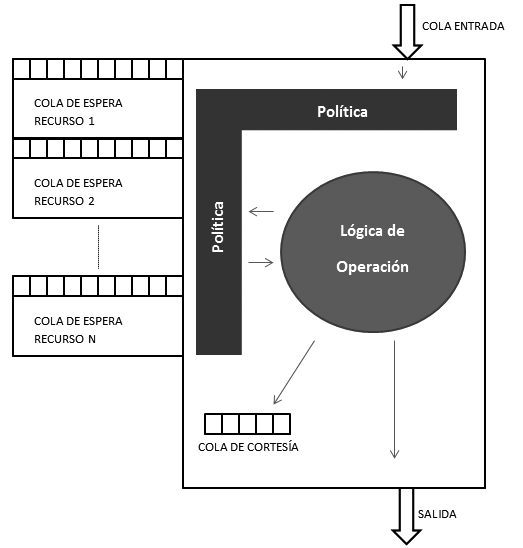
\includegraphics[width=1\linewidth,keepaspectratio]{./marco_teorico/concurrencia/img/concurrencia04}
			\caption{Monitor}
			\label{fig:concurrencia04}
		\end{figure}
		
 				% FPGA - IP core - HDL
 					%%%%%%%%%%%%%%%%%%%%%%%%%%%%%%%%%%%%%%%%%%%%%%%%%%%%%%%%%%%%%%%%%%%%%%%%%%%%%%%%
%	TRABAJO: Proyecto Integrador
%		Titulo: 	Desarrollo de IP cores con procesamiento de Redes de Petri 	
%					Temporales para sistemas multicore en FPGA					
%		Autores:	Juli�n Nonino												%					Carlos Renzo Pisetta										%		Director:	Orlando Micolini											
%%%%%%%%%%%%%%%%%%%%%%%%%%%%%%%%%%%%%%%%%%%%%%%%%%%%%%%%%%%%%%%%%%%%%%%%%%%%%%%%

% Path im�genes: ./marco_teorico/FPGA_IP_HDL/img
% Nombre predeterminado im�genes: fpgaxx
%	xx es el numero de imagen

\chapter{FPGA - IP cores - HDL}
	\label{chap:chap_fpga_ip_hdl}
	
	El objetivo de esta secci�n, es introducir al lector en los conceptos de FPGA, IP core y HDL. Para ello, se comenzar� explicando brevemente qu� es una Field Programmable Gate Array (FPGA) y sus posibles usos. Luego, se continua con el concepto de IP Core, su clasificaci�n y algunos IP Cores que ser�n utilizados a lo largo de este trabajo. Para finalizar, se brindar� una introducci�n al lenguaje Verilog para que el lector adquiera las nociones b�sicas para entender la implementaci�n de este trabajo.

	% FPGA
		%%%%%%%%%%%%%%%%%%%%%%%%%%%%%%%%%%%%%%%%%%%%%%%%%%%%%%%%%%%%%%%%%%%%%%%%%%%%%%%%
%	TRABAJO: Proyecto Integrador
%		Titulo: 	Desarrollo de IP cores con procesamiento de Redes de Petri 	
%					Temporales para sistemas multicore en FPGA					
%		Autores:	Juli�n Nonino												%					Carlos Renzo Pisetta										%		Director:	Orlando Micolini											
%%%%%%%%%%%%%%%%%%%%%%%%%%%%%%%%%%%%%%%%%%%%%%%%%%%%%%%%%%%%%%%%%%%%%%%%%%%%%%%%

% Path im�genes: ./marco_teorico/FPGA_IP_HDL/img
% Nombre predeterminado im�genes: fpgaxx
%	xx es el numero de imagen

\section{Field Programmable Gate Array}
	\label{sec:fpga}

	Una FPGA (Field Programmable Gate Array) es un circuito integrado digital formado por bloques l�gicos los interconectados.

	Las interconexiones de una FPGA pueden ser conFigurados mediante un Lenguaje de Descripci�n de Hardware (HDL). De esta manera una FPGA puede reproducir desde simples compuertas l�gicas hasta complejos sistemas dentro de un solo chip.

	Existen FPGAs que pueden ser reprogramadas lo que les permite una gran flexibilidad a la hora de dise�ar circuitos digitales. Por otro lado, existen FPGAs que solo pueden programarse una �nica vez, su principal ventaja su menor consumo aunque al momento de dise�ar circuitos son mas complejas.

	En la \ref{fig:fpga01} se ve una FPGA dentro de una placa de desarrollo con diferentes perif�ricos ya conectados.
	
	Las caracter�sticas f�sicas a tener en cuenta en la elecci�n de una FPGA depender�n del proyecto que se desea emprender, pero, principalmente se consideran los siguientes puntos:
	\begin{itemize}
	  \item \emph{Cantidad de bloques l�gicos}: determina el espacio disponible para implementar la l�gica.
	  \item \emph{Tipo y tama�o de memoria}: pudiendo ser \emph{distribuida} o \emph{de bloques}, donde existe una memoria dedicada incluida en la FPGA o se utilizan los bloques l�gicos de la misma respectivamente.
	  \item \emph{Cantidad de puertos I/O}: usados como interface entre la FPGA y dispositivos externos.
	  \item \emph{Otros componentes internos}: Bloques de memoria, multiplicadores, PLL, CPU, conversores A/D, bloques DSP, etc.
	\end{itemize}
	
	\begin{raggedright}
	Las FPGA ofrecen las siguientes ventajas:
	\end{raggedright}	
	\begin{itemize}
		\item Gran flexibilidad de producto.
		\item Posibilidad de actualizar tanto el firmware como el hardware.
		\item Reutilizaci�n del hardware.
		\item Son dispositivos reconfigurables.
		\item Bajo costo respecto a los ASIC.
		\item Ejecuci�n de circuitos m�s r�pida que en otros dispositivos reprogramables.
		\item \textbf{La ejecuci�n de cada bloque se realiza concurrentemente, a diferencia de un micro controlador.}
		\item Gran utilidad para dise�o y testing de prototipos. 
	\end{itemize}
	\begin{raggedright}
		Por otro lado, tienen las siguientes desventajas:
	\end{raggedright}
	\begin{itemize}
		\item M�s costosas que los microprocesadores equivalentes.
		\item Mayor complejidad de dise�o (soft+hard).
		\item Retardos de propagaci�n mayores a los existentes en ASIC (Application Specific Integrated Circuit).
		\item Mayores costos en producci�n a gran escala.
		\item Consumo est�tico y din�mico moderados.
	\end{itemize}	
	\begin{figure}[H]
		\centering
		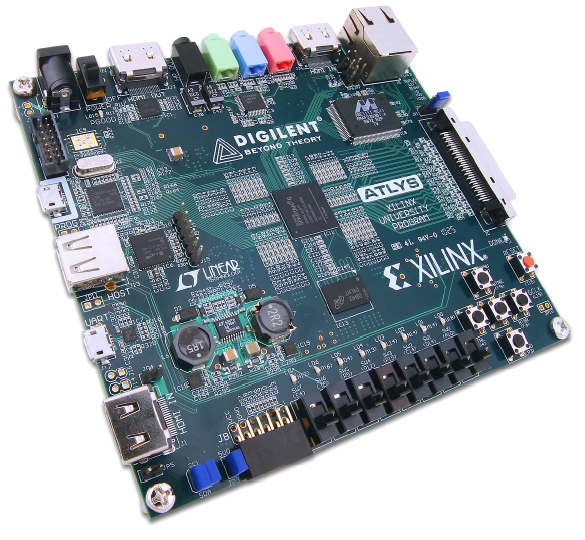
\includegraphics[width=.4\linewidth]{./marco_teorico/FPGA_IP_HDL/img/fpga01}
		\caption{Atlys Spartan-6 FPGA Development Board}
		\label{fig:fpga01}
	\end{figure}
	\newpage
		
	% IP cores
		%%%%%%%%%%%%%%%%%%%%%%%%%%%%%%%%%%%%%%%%%%%%%%%%%%%%%%%%%%%%%%%%%%%%%%%%%%%%%%%%%%%%%
%																					%
%	TRABAJO: Proyecto Integrador													%
%																					%
%		Titulo: 	Desarrollo de IP cores con procesamiento de Redes de Petri 		%
%					Temporales para sistemas multicore en FPGA						%
%																					%
%		Autores:	Juli�n Nonino													%
%					Carlos Renzo Pisetta											%
%		Director:	Orlando Micolini												%
%																					%
%	Parte: Marco Teorico															%
%	Capitulo: FPGA - IP cores - HDL													%
%	Seccion: Intellectual Property (IP) Core										%	
%	Archivo: ip_cores.tex															%
%																					%
%%%%%%%%%%%%%%%%%%%%%%%%%%%%%%%%%%%%%%%%%%%%%%%%%%%%%%%%%%%%%%%%%%%%%%%%%%%%%%%%%%%%%

% Path Imagenes: ./marco_teorico/FPGA_IP_HDL/img
% Nombre predeterminado imagenes: fpgaxx
%	xx es el numero de imagen


\section{Intellectual Property (IP) Core}
	\label{sec:ip_cores}

	Un \textbf{\emph{IP Core (Intellectual Property Core)}} es un bloque o m�dulo idealmente parametrizable 
	y reutilizable para usar en dise�os de FPGA o en ASIC. Posee una funcionalidad predefinida y es creado 
	con el uso de est�ndares, independizandolo de la herramienta de desarrollo.
	Los IP cores  se pueden licenciar en base a su funcionalidad. Existen dise�os de microprocesadores (soft-CPU) 
	o controladores de perif�ricos como USB, PCI, SDRAM, etc.
	
	Se puede clasificar un IP Core principalmente en tres categor�as:
	\begin{itemize}
	  \item \textbf{Hard Core:} Est�n dise�ados para una tecnolog�a espec�fica, tienen mejor 
	  		desempe�o y no pueden ser modificados por el dise�ador que los utiliza. Son poco 
	  		flexibles, portables y conFigurables pero son muy predecibles y fiables una vez 
	  		implementados. Tienen un layout predefinido incluido en la arquitectura.
	  \item \textbf{Firm Core:} Al igual que los \emph{hard}, incluyen informaci�n del mapeo a nivel 
	  		de compuertas y el c�digo fuente es visible para el dise�ador, haci�ndolos parcialmente 
	  		conFigurables. Suelen ser dise�ados y probados en diferentes tecnolog�as especificas, 
	  		ofreciendo una buena predictibilidad en cuanto a performance de tiempos de funcionamiento 
	  		y �rea utilizada, pero el usuario se ver� obligado a utilizar estos sobre las placas del 
	  		mismo fabricante.
	  \item \textbf{Soft Core:} Son los m�s flexibles y se distribuyen en c�digo de alto nivel HDL 
	  		permitiendo a los dise�adores modificarlo. Otro formato es mediante las netlist o lista 
	  		de compuertas e interconexiones. Ambos formatos los hace independientes de la tecnolog�a.
	\end{itemize}
	
	\begin{raggedright}
		\begin{tabular}{|p{2.5cm}||p{4cm}|p{4cm}|p{4cm}|}
			\hline
				& Hard Core & Firm Core & Soft Core\\
			\hline
			\hline
				Adaptabilidad & 
				Layout predefinido & 
				Mezcla de c�digo fuente y tecnolog�a dependiente de la netlist &	
				Dependiente del comportamiento del c�digo\\
			\hline
				Modelado & 
				Modelado como librer�a de elementos &
				Mezcla de bloques fijos y sintetizables que pueden ser compartidos por otros cores &
				Sintetizable con otra l�gica.\\
			\hline
				Flexibilidad & 
				No puede ser modificado por el dise�ador. Utilizar varios de �stos cores en un chip puede 
				resultar ineficiente. &
				Tecnolog�a dependiente.&
				El dise�o puede variarse.\\
			\hline
				Predictibilidad	&
				Garantiza los timing. &
				Camino critico es fijo. &
				Timing no garantizado.\\
			\hline
				Coste &	Bajo & Medio & Alto\\
			\hline
				Descripci�n &
				Ficheros layout y timing information. &
				C�digo sintetizable HDL y ficheros layout y timing information. &
				C�digo sintetizable HDL. \\
			\hline
		\end{tabular}
	\end{raggedright}
	\newpage
	Basados en estas caracter�sticas, se planteo desarrollar un \emph{Soft Core} debido a su gran 
	flexibilidad que permite futuras modificaciones.
		
	\subsection{MicroBlaze}
		
		El MicroBlaze \cite{xilinx_microblaze} es un procesador \emph{soft core} creado por Xilinx. Tiene 
		un set de instrucciones reducido (RISC) y esta optimizado para ser instanciado en una FPGA.
		\begin{figure}[H]
			\centering
			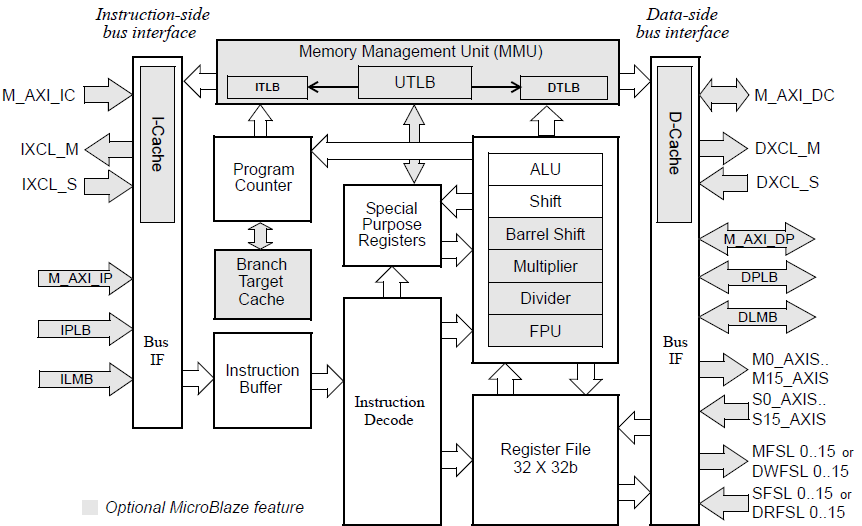
\includegraphics[width=0.9\linewidth]{./marco_teorico/FPGA_IP_HDL/img/fpga02}
			\caption{Diagrama en bloques de un core MicroBlaze}
			\label{fig:fpga02}
		\end{figure}
		
		\subsubsection{Caracter�sticas b�sicas}
			
			El MicroBlaze tiene las siguientes caracter�sticas fijas, es decir, no modificables.
			\begin{itemize}
			  	\item 32 de registros de 32 bits cada uno.
			  	\item Instrucciones de 32 bits con tres operandos y dos modos de direccionamiento.
			  	\item Bus de direcciones de 32 bits.
			\end{itemize}
			
			El resto de las caracter�sticas, pueden ser conFiguradas al momento de instanciarlo.
		
		\subsubsection{Endianismo}
			
			El MicroBlaze puede usar el formato Big-Endian o Little-Endian para representan los datos.
			La elecci�n depende del valor de un par�metro llamado: \emph{C\_ENDIANNESS}. 
			\\
			
			Los tipos de datos soportados por el procesador son:
			\begin{itemize}
			  	\item Word (32 bits).
			  	\item Half Word (16 bits).
			  	\item Byte (8 bits).  
			\end{itemize}
			 
		\subsubsection{Instrucciones}
			
			Las instrucciones del MicroBlaze se clasifican en dos tipos.
			\begin{itemize}
			  	\item \emph{Tipo A}: Toma dos operandos como fuente y uno como destino.
			  	\item \emph{Tipo B}: Toma un �nico operando como fuente, un operador inmediato de 16 
			  		bits y uno como registro destino. El operador de 16 bits puede ser convertido a 32 
			  		bits precediendo la instrucci�n tipo B con una instrucci�n ``Imm".
			\end{itemize}
		
		\subsubsection{Pipeline}
		
			El MicroBlaze ejecuta sus instrucciones de forma segmentada. Para la mayor�a de las instrucciones 
			cada etapa del pipeline toma un ciclo. Algunas pocas necesitan m�s de un ciclo en la etapa de 
			ejecuci�n, para	ello, se detiene el pipeline los ciclos necesarios.En general, se completa una 
			instrucci�n por ciclo.
			\\
			
			El pipeline del MicroBlaze puede ser de tres o cinco etapas dependiendo de la disponibilidad de 
			hardware que se tenga.
			\\
			
			Con el par�metro \emph{C\_AREA\_OPTIMIZED} en \emph{1} (uno), el pipeline se divide en tres etapas:
			\begin{enumerate}
			  	\item B�squeda de instrucci�n.
			  	\item Decodificaci�n de instrucci�n.
			  	\item Ejecuci�n de instrucci�n.
			\end{enumerate}
			
			
			Con el par�metro \emph{C\_AREA\_OPTIMIZED} en \emph{0} (cero), el pipeline se divide en cinco etapas:
			\begin{enumerate}
			  	\item B�squeda de instrucci�n.
			  	\item Decodificaci�n de instrucci�n.
			  	\item Ejecuci�n de instrucci�n.
			  	\item Accesos a memoria.
			  	\item Writeback.
			\end{enumerate}
		
		\newpage
		
		\subsubsection{Interfaces de conexi�n}
			
			El MicroBlaze soporta cuatro interfaces de conexi�n con perif�ricos: \emph{Local Memory Bus (LMB)},
			\emph{AMBA� AXI4 interface (AXI4)}, \emph{IMB Processor Local Bus (PLB)} y \emph{Xilinx CacheLink (XCL)}.
			
			El Local Memory Bus (LMB). Sirve para proveer acceso de un solo ciclo a una memoria block RAM 
			de dos puertos ubicada on-chip.
			
			Los buses AXI4 y PLB proveen conexiones a perif�ricos on-chip y off-chip adem�s de con la memoria.
			
			La interface CacheLink fue creada para usar con controladores de memoria externos.
			
			El MicroBlaze tambi�n soporta 16 puertos para interfaces Fast Simplex Link (FLS) o 4 AXI4-Stream. 
			Cada una con una interface master y una slave.
		
	\subsection{AXI}
	
		El \textbf{Advanced eXtensible Interface} (AXI) \cite{xilinx_axi} es un IP core que permite la 
		conexi�n entre IP cores. Puede tener hasta 16 IP cores de cada tipo conectados simult�neamente. Cada 
		uno puede usar anchos de datos de 32, 64, 128, 256, 512, 1024 independientemente del resto. El bus de 
		direcciones puede variar entre 12 y 64 bits.
	
		\subsubsection{Diagrama funcional}
		
			El \textbf{AXI Interconnect core} \ref{fig:fpga03} esta compuesto por dos interfaces, la interface 
			esclavo (slave), donde seconectan los dispositivos master y una interface maestro (master) donde se 
			conectan los dispositivos slave. Entre estas interfaces existen varias unidades funcionales divididas 
			en dos grupos, uno por cada Interface. En el medio se encuentra la crossbar encargada del ruteo de 
			peticiones entre los distintos dispositivos.
			\begin{figure}[H]
				\centering
				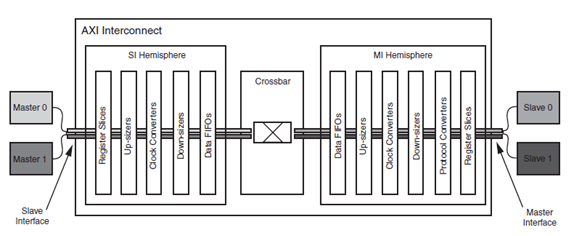
\includegraphics[width=0.95\linewidth]{./marco_teorico/FPGA_IP_HDL/img/fpga03}
				\caption{Diagrama de interconexi�n AXI}
				\label{fig:fpga03}
			\end{figure}
		\newpage
		\subsubsection{Tipos de conexi�n}
			El bus AXI permite la conexi�n entre IP cores master con los slave de las siguientes maneras:
			\begin{itemize}
			  	\item \textbf{Pass through}
			  		Este modo se utiliza cuando solo un master y un esclavo se conectan y no se utiliza ninguna 
					de las unidades funcionales de las que dispone el AXI.
			  		\begin{figure}[H]
						\centering
						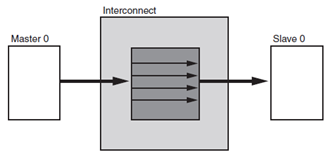
\includegraphics[width=.6\linewidth]{./marco_teorico/FPGA_IP_HDL/img/fpga04}
						\caption{Conexi�n AXI pass through}
						\label{fig:fpga04}
					\end{figure}
			  		
			  	\item \textbf{Conversion only}
			  		
			  		Este modo es conecta un master con un esclavo pero habilitando una o mas unidades funcionales 
					permitiendo conversi�n o funciones de pipeline. Las posibles unidades son:
					\begin{itemize}
						\item Conversi�n de tama�o de dato.
						\item Conversi�n de clock rate.
						\item Adaptaci�n de esclavo AXI4-Lite.
						\item Adaptaci�n de esclavo AXI-3.
						\item Pipelining, como registros de desplazamiento o canales de datos FIFO.
					\end{itemize}
					\begin{figure}[H]
						\centering
						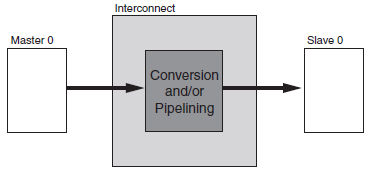
\includegraphics[width=.6\linewidth]{./marco_teorico/FPGA_IP_HDL/img/fpga05}
						\caption{Conexi�n AXI conversion only}
						\label{fig:fpga05}
					\end{figure}
			  	
			  	\item \textbf{N to 1 interconnect}
			  		
			  		Otro modo de usarlo es conectar m�ltiples masters a un �nico dispositivo esclavo. En este caso
					la decodificaci�n de direcciones es omitida salvo que la validaci�n de rango sea necesaria. En
					cualquier caso las conversiones de tama�o de dato o clock rate  pueden ser utilizadas.	
					\begin{figure}[H]
						\centering
						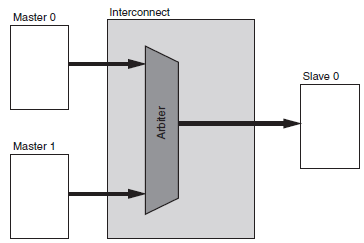
\includegraphics[width=.7\linewidth]{./marco_teorico/FPGA_IP_HDL/img/fpga06}
						\caption{Conexi�n AXI N to 1 interconnect}
						\label{fig:fpga06}
					\end{figure}
				
			  	\item \textbf{1 to N interconnect}
			
					Otro modo de uso valido es la conexi�n de un Master controlando varios esclavos. En este caso 
					el arbitraje de direcciones y escritura de datos no se realiza.
					\begin{figure}[H]
						\centering
						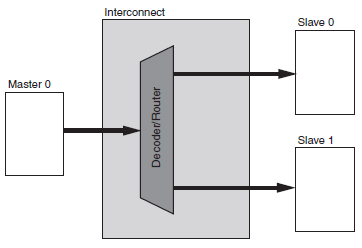
\includegraphics[width=.7\linewidth]{./marco_teorico/FPGA_IP_HDL/img/fpga07}
						\caption{Conexi�n AXI N to 1 interconnect}
						\label{fig:fpga07}
					\end{figure}
			  	
			  	\item \textbf{N to M interconnect (Crossbar)}
			
					En este modo se usa una topolog�a de direcci�n compartida y m�ltiples datos (SAMD). Consiste 
					en una crossbar para la escritura/lectura de datos y �rbitros para las direcciones.
					Existen caminos paralelos para escribir y leer por los cuales cualquier master puede acceder 
					a cualquier esclavo. Cuando m�s de una fuente accede a diferentes destinos se pueden realizar 
					estas operaciones de forma simult�nea.
					\begin{figure}[H]
						\centering
						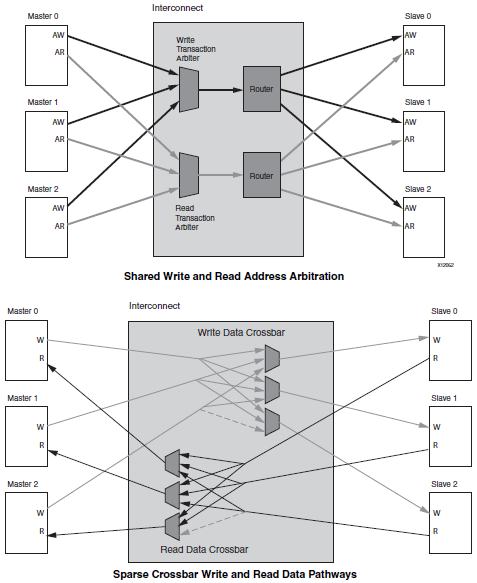
\includegraphics[width=0.8\linewidth]{./marco_teorico/FPGA_IP_HDL/img/fpga08}
						\caption{Conexi�n AXI N to M interconnect (Crossbar)}
						\label{fig:fpga08}
					\end{figure}
			  	
			  	\item \textbf{N to M interconnect (Shared Access)}
			
					En el modo compartido solo se puede realizar una transacci�n a la vez. Para cada master 
					conectado un pedido de lectura tiene prioridad sobre uno de escritura. El �rbitro selecciona 
					la solicitud a realizar entre las existentes. Este modo minimiza los recursos usados para 
					implementar el modulo de crossbar.
					\begin{figure}[H]
						\centering
						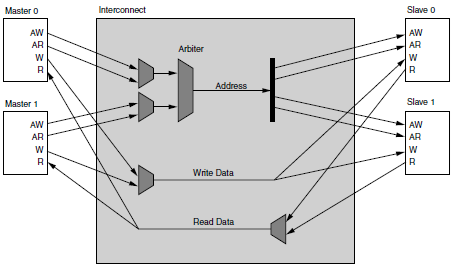
\includegraphics[width=.8\linewidth]{./marco_teorico/FPGA_IP_HDL/img/fpga09}
						\caption{Conexi�n AXI N to M interconnect (Shared Access)}
						\label{fig:Shared}
					\end{figure}	
			\end{itemize}
	
	
	% HDL
		%%%%%%%%%%%%%%%%%%%%%%%%%%%%%%%%%%%%%%%%%%%%%%%%%%%%%%%%%%%%%%%%%%%%%%%%%%%%%%%%%%%%%
%																					%
%	TRABAJO: Proyecto Integrador													%
%																					%
%		Titulo: 	Desarrollo de IP cores con procesamiento de Redes de Petri 		%
%					Temporales para sistemas multicore en FPGA						%
%																					%
%		Autores:	Juli�n Nonino													%
%					Carlos Renzo Pisetta											%
%					Orlando Micolini												%
%																					%
%	Parte: Marco Teorico															%
%	Capitulo: FPGA - IP cores - HDL													%
%	Seccion: Hardware Description Language (HDL)									%	
%	Archivo: hdl.tex																%
%																					%
%%%%%%%%%%%%%%%%%%%%%%%%%%%%%%%%%%%%%%%%%%%%%%%%%%%%%%%%%%%%%%%%%%%%%%%%%%%%%%%%%%%%%

% Path Imagenes: ./marco_teorico/FPGA_IP_HDL/img
% Nombre predeterminado imagenes: fpgaxx
%	xx es el numero de imagen

\lstset
{	language=Verilog,               % the language of the code
	basicstyle=\footnotesize,       % the size of the fonts that are used for the code
	numbers=left,                   % where to put the line-numbers
	numberstyle=\tiny\color{gray},  % the style that is used for the line-numbers
	stepnumber=1,                   % the step between two line-numbers. If it's 1, each line 
                       				% will be numbered
	numbersep=5pt,                  % how far the line-numbers are from the code
	backgroundcolor=\color{white},  % choose the background color. You must add \usepackage{color}
	showspaces=false,               % show spaces adding particular underscores
	showstringspaces=false,         % underline spaces within strings
	showtabs=false,                 % show tabs within strings adding particular underscores
	frame=none,                 	% adds a frame around the code
	rulecolor=\color{white},        % if not set, the frame-color may be changed on line-breaks within not-black text (e.g. comments (green here))
	tabsize=2,                      % sets default tabsize to 2 spaces
	captionpos=b,                   % sets the caption-position to bottom
	breaklines=true,                % sets automatic line breaking
	breakatwhitespace=false,        % sets if automatic breaks should only happen at whitespace
	%title=\lstname,                % show the filename of files included with \lstinputlisting;
		                            % also try caption instead of title
	keywordstyle=\color{blue},      % keyword style
  	commentstyle=\color{dkgreen},   % comment style
  	stringstyle=\color{mauve},      % string literal style
  	escapeinside={\%*}{*)},         % if you want to add LaTeX within your code
  	morekeywords={*,...},           % if you want to add more keywords to the set
  	deletekeywords={...}            % if you want to delete keywords from the given language
}

\section{Hardware Description Language (HDL)}
	\label{sec:hdl}

		Un lenguaje de descripci�n de hardware (HDL) permite definir las interconexiones y el comportamiento 
		de un circuito electr�nico y verificar el funcionamiento mediante simulaciones.
		 	
		\subsection{Verilog}
			
			Verilog \cite{ashenden}, es un HDL definido en un est�ndar de IEEE que soporta el dise�o, prueba e 
			implementaci�n de circuitos a diferentes niveles de abstracci�n. Su sintaxis es similar al del 
			lenguaje de programaci�n \emph{C}.

			\subsubsection{Verilog como lenguaje}
			
				El dise�o se describe como un conjunto de m�dulos. Utilizando la palabra clave \textbf{module}
				se define un m�dulo y se pueden especificar sus entradas y salidas y finalizan con una 
				sentencia endmodule como se muestra a continuaci�n:
				\begin{lstlisting}
module AOI (input A, B, C, D, output F)
	... descripci�n de funcionamiento ...
endmodule	
				\end{lstlisting}
				
			\begin{raggedright}
			Cada m�dulo es una unidad l�gica que incluye:
			\end{raggedright}
			\begin{itemize}
				\item Una interfaz para su conexi�n con otros m�dulos.
			  	\item Una descripci�n de su contenido mediante la especificaci�n de su comportamiento
			\end{itemize}
						
			El sentido de las conexiones con otros m�dulos puede ser de tres tipos, entradas (\emph{input}), 
			salidas (\emph{output}) o entrada-salida (\emph{inout}). Una vez que se ha definido el m�dulo se 
			puede instanciar cuantas veces sea necesario en el dise�o.
			
			Cada ejemplar del m�dulo que se utilice son elementos distintos por lo que se deben definir sus 
			conexiones con otros m�dulos.
			\\
			
			Verilog tiene b�sicamente dos tipos de datos. Por un lado, los \emph{par�metros}, estos, son constantes 
			definidas por el programador que no son implementadas en hardware pero ayudan a la descripci�n del
			comportamiento. 
			
			Por otro lado, las \emph{variables} y los \emph{registros}. Las variables se utilizan para 
			almacenar valores, pero esto no implica que se vean expl�citamente en la implementaci�n de hardware.
			
			Existen adem�s, los denominados \emph{wire} los cuales no retienen informaci�n, su funci�n es comunicar dos 
			o mas puntos de los cuales uno solo es el driver, es decir, el que puede modificar el estado 
			l�gico del cable.
			
			\subsubsection{L�gica de estados}
			
				Una variable en Verilog no solamente se representa con un $0$ y $1$, maneja una l�gica de cuatro 
				estados, los registros como wires pueden estar en uno de los siguientes:
				\begin{itemize}
					\item \textbf{X}: desconocido.
					\item \textbf{0}: false o nivel cero.
					\item \textbf{1}: true o nivel 1.
					\item \textbf{Z}: alta impedancia. 
				\end{itemize}
			
			\subsubsection{Buses}

				Los \emph{buses} o \emph{arrays} son elementos de varios bits que pueden ser del tipo \emph{wire} 
				o \emph{reg}. Los buses pueden ser usados como interfaz con otros m�dulos. A la hora de declararlos 
				se puede elegir la orientaci�n de los bits, es decir, \emph{MSB} el \emph{n} bit o \emph{MSB} el bit 
				\emph{0}, como se muestra en la Figura \ref{fig:fpga10}.
				\begin{figure}[H]
					\centering
					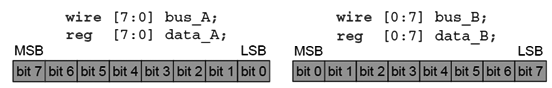
\includegraphics[width=.8\linewidth]{./marco_teorico/FPGA_IP_HDL/img/fpga10}
					\caption{Definici�n de buses en Verilog}
					\label{fig:fpga10}
				\end{figure}
				
				Las \emph{matrices} son un tipo de \emph{array de array} los cuales tienen la siguiente sintaxis de 
				definici�n.
				\begin{lstlisting}
reg [7:0] mem [0:3];
				\end{lstlisting}
				
				En ellas, se aplican las mismas definiciones de orden que para los array pero no pueden ser 
				usadas como interfaces con otros m�dulos.
			
			\subsubsection{Operadores}
				
				\begin{raggedright}
					\textbf{\emph{Operadores Binarios Aritm�ticos}}
				\end{raggedright}
				
				Existen cinco operadores aritm�ticos. Un detalle de su operaci�n es que si alg�n bit esta en 
				un estado desconocido el resultado tambi�n lo estar�.
				\begin{itemize}
				  	\item \textbf{\emph{+}} (\emph{suma o signo positivo}):
				  		Sirve para indicar una suma entre dos n�meros.
						\begin{lstlisting}
// B: 4'b1000   C: 4'b10
	A = B + C;
//Resultado A: 4'b1010
						\end{lstlisting}
				  	\item \textbf{\emph{-}} (\emph{resta o signo negativo}):
				  		Sirve para indicar la resta entre dos n�meros.
				  		\begin{lstlisting}
// B: 4'b1000   C: 4'b10
	A = B - C;
// Resultado A: 4'b0110
						\end{lstlisting}
				  	\item \textbf{\emph{*}} (\emph{multiplicaci�n}):
				  		Multiplica dos n�meros de cualquier tipo.
				  		\begin{lstlisting}
// B: 4'b0100   C: 4'b10
	A = B * C;
// Resultado A: 4'b1000
						\end{lstlisting}
				  	\item \textbf{\emph{/}} (\emph{divisi�n}):
				  		Divide dos n�meros de cualquier tipo.
				  		\begin{lstlisting}
// B: 4'b1000   C: 4'b10
	A = B / C;
// Resultado A: 4'b0100
						\end{lstlisting}
				  	\item \textbf{\emph{\%}} (\emph{resto}):
				  		Obtiene el resto de la divisi�n de dos n�meros de cualquier tipo.
				  		\begin{lstlisting}
// B: 4'b1000   C: 4'b10
	A = B \% C;
// Resultado A: 4'b0000
						\end{lstlisting}
				\end{itemize}

				\begin{raggedright}
					\textbf{\emph{Operadores de Igualdad}}
				\end{raggedright}
				
				Permiten comparar dos operandos, retornando $1$ � $0$, verdadero o falso respectivamente.
				\begin{itemize}
				  	\item \textbf{\emph{==, !=}} (\emph{igualdad}):
				  		El primero devuelve verdadero si los operando son iguales y falso en caso contrario. 
				  		El segundo indica desigualdad, funcionando al rev�s que el anterior. Si alg�n bit est� 
				  		en estado desconocido el resultado tambi�n lo estar�.
						\begin{lstlisting}
// A: 4'b1110   B: 4'b1101
	if (B != A)
//Resultado = true
						\end{lstlisting}
				  	\item \textbf{\emph{===, !==}} (\emph{igualdad}):
				  		Su funcionalidad es id�ntica a la anterior, pero difiere en tambi�n se comparan los valores 
				  		indefinidos ($X$) o de alta impedancia ($Z$).
				  		\begin{lstlisting}
// A: 4'b11X0   B: 4'b11X0
	if (B === A)
// Resultado = true
						\end{lstlisting}
				\end{itemize}				

				\begin{raggedright}
					\textbf{\emph{Operadores Relacionales}}
				\end{raggedright}
							
				Permiten comparar dos operandos, retornando $1$ � $0$, verdadero o falso respectivamente. Si 
				alg�n bit es $X$ el resultado tambi�n ser� $X$.
				
				\begin{itemize}
				  	\item \textbf{\emph{$>, \geq, <, \leq$}} (\emph{mayor, menor}):
				  		Poseen el significado habitual (mayor que, mayor o igual que, menor que, menor o igual que, 
						respectivamente).
						\begin{lstlisting}
// A: 4'b1110   B: 4'b1101
	if (B > A)
// Resultado = false
						\end{lstlisting}
				\end{itemize}
		
				\begin{raggedright}
					\textbf{\emph{Operadores L�gicos}}
				\end{raggedright}
				
				Aparecen entre dos operandos l�gicos y proporciona un valor l�gico (verdadero o falso).
				\begin{itemize}
				  	\item \textbf{\emph{!}} (\emph{negaci�n}):
				  		Cambia el valor l�gico del operando que va justo detr�s del operador.
				  		\begin{lstlisting}
// A = true
	if (!A)
// Resultado = false
						\end{lstlisting}
				  	\item \textbf{\emph{$\&\&$}} (\emph{AND l�gica}):
				  		El resultado ser� la combinaci�n de los dos operandos l�gicos. Es decir, para que 
				  		el valor sea verdadero, ambos operandos deben serlo, en caso contrario el resultado
				  		ser� falso.
				  		\begin{lstlisting}
// A = true ; B = false
	if (A && B)
// Resultado = false
						\end{lstlisting}
				  	\item \textbf{\emph{$\mid\mid$}} (\emph{OR logica}):
				  		El resultado ser� la combinaci�n de los dos operandos l�gicos. Para que el resultado sea 
				  		verdadero, bastar� con que uno de los operandos lo sea.
				  		\begin{lstlisting}
// A = true ; B = false
	if (A || B)
// Resultado = true
						\end{lstlisting}
				\end{itemize}

				\begin{raggedright}
					\textbf{\emph{Operadores L�gicos a nivel de bit}}
				\end{raggedright}
				
				Permite efectuar operaciones l�gicas con los bits de los operandos.	
				\begin{itemize}
					\item \textbf{\emph{$\sim$}} (\emph{negaci�n}):
				  		Negaci�n bit a bit.
				  		\begin{lstlisting}
// B: 4'b1110
	A = ~B;
// Resultado: A = 4'b0001
						\end{lstlisting}
					\item \textbf{\emph{$\&$}} (\emph{AND}):
						AND bit a bit.
						\begin{lstlisting}
// B: 4'b1110   C: 4'b1101
	A = B & C;
// Resultado: A = 4'b1100
						\end{lstlisting}
					\item \textbf{\emph{$\mid$}} (\emph{OR}):
						OR bit a bit.
						\begin{lstlisting}
// B: 4'b1110   C: 4'b1101
	A = B | C;
// Resultado: A = 4'b1111
						\end{lstlisting}
					\item \textbf{\emph{$\wedge$}} (\emph{XOR}):
						XOR bit a bit.
						\begin{lstlisting}
// B: 4'b1110   C: 4'b1101
	A = B ^ C;
// Resultado: A = 4'b0011
						\end{lstlisting}
					\item \textbf{\emph{$\sim\&$}} (\emph{NAND}):
						NAND bit a bit.
						\begin{lstlisting}
// B: 4'b1110   C: 4'b1101
	A = B ~& C;
// Resultado: A = 4'b0011
						\end{lstlisting}
					\item \textbf{\emph{$\sim\mid$}} (\emph{NOR}):
						NOR bit a bit.
						\begin{lstlisting}
// B: 4'b1110   C: 4'b1101
	A = B ~| C;
// Resultado: A = 4'b0000
						\end{lstlisting}
					\item \textbf{\emph{$\sim\wedge$}} (\emph{NOT XOR}):
						NOT XOR bit a bit. Tambi�n puede ser $\wedge\sim$.
						\begin{lstlisting}
// B: 4'b1110   C: 4'b1101
	A = B ~^ C;
// Resultado: A = 4'b1100
						\end{lstlisting}	
				\end{itemize}
				
				\begin{raggedright}
					\textbf{\emph{Operadores L�gicos de reducci�n}}
				\end{raggedright}
				
				El resultado de aplicar este operando al �nico argumento es un s�lo bit.	
				\begin{itemize}
				  	\item \textbf{\emph{$\&$}} (\emph{AND}):
						Se realiza un AND de todos los bits.
						\begin{lstlisting}
// B: 4'b1110
	A = &B;
// Resultado: A = 1'b0
						\end{lstlisting}
					\item \textbf{\emph{$\mid$}} (\emph{OR}):
						Se realiza un OR entre todos los bits del operando.
						\begin{lstlisting}
// B: 4'b1110
	A = |B;
// Resultado: A = 1'b1
						\end{lstlisting}
					\item \textbf{\emph{$\wedge$}} (\emph{XOR}):
						Se realiza un XOR entre todos los bits del operando.
						\begin{lstlisting}
// B: 4'b1110
	A = ^B;
// Resultado: A = 1'b1
						\end{lstlisting}
					\item \textbf{\emph{$\sim\&$}} (\emph{NAND}):
						Se realiza un NAND de todos los bits.
						\begin{lstlisting}
// B: 4'b1110
	A = ~&B;
// Resultado: A = 1'b1
						\end{lstlisting}
					\item \textbf{\emph{$\sim\mid$}} (\emph{NOR}):
						Se realiza un NOR entre todos los bits del operando.
						\begin{lstlisting}
// B: 4'b1110
	A = ~|B;
// Resultado: A = 1'b0
						\end{lstlisting}
					\item \textbf{\emph{$\sim\wedge$}} (\emph{NOT XOR}):
						Se realiza un NOT XOR entre todos los bits del operando. Tambi�n puede ser $\wedge\sim$.
						\begin{lstlisting}
// B: 4'b1110
	A = ~^B;
// Resultado: A = 1'b0
						\end{lstlisting}
				\end{itemize}
					  		
	  			\begin{raggedright}
					\textbf{\emph{Otros Operadores}}
				\end{raggedright}		
	  			
	  			\begin{itemize}
				  	\item \textbf{\emph{$\{,\}$}} (\emph{Concatenaci�n}):
				  		Concatenaci�n de dos operandos.
				  		\begin{lstlisting}
// B = 4'b0110  C = 4'b0010
	A = {B,C};  		// Resultado: A = 8'b01100010
	D = {2{B}}; 		// Resultado: D = 8'b01100110
	E = {B,C[1:0]}; // Resultado: E = 6'b011010}
						\end{lstlisting}
					
					\newpage	
						
				  	\item \textbf{\emph{$<<$}} (\emph{Desplazamiento izquierda}):
				  		Desplaza bits a la izquierda, a�adiendo ceros.
				  		\begin{lstlisting}
// A = 8'b11101101
	A << 2;  		
// Resultado: A = 8'b10110100
						\end{lstlisting}
				  	\item \textbf{\emph{$>>$}} (\emph{Desplazamiento derecha}):
				  		Desplaza bits a la derecha, a�adiendo ceros.
				  		\begin{lstlisting}
// A = 8'b11101101
	A >> 3;  		
// Resultado: A = 8'b00011101
						\end{lstlisting}
				  	\item \textbf{\emph{?}} (\emph{Condicional}):
				  		Dependiendo del resultado l�gico (verdadero o falso) se devolver� un valor u otro.
				  		\begin{lstlisting}
// A = 1'b1  B = 3'b111  C = 3'b001
	A == 1 ? B : C;	
// Resultado: A = 3'b111
						\end{lstlisting}
	  			\end{itemize}
	  			
			\subsubsection{Asignaciones}
				
				Existen dos tipos de asignaciones, por un lado est�n las bloqueantes las cuales se asemejan 
				a los cables simbolizadas con el $=$ como se muestra en la Figura \ref{fig:fpga11}.
					\begin{figure}[H]
						\centering
						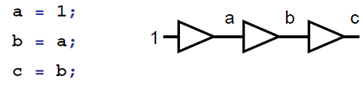
\includegraphics[width=.5\linewidth]{./marco_teorico/FPGA_IP_HDL/img/fpga11}
						\caption{Asignaci�n bloqueante en Verilog}
						\label{fig:fpga11}
					\end{figure}
				
				Por otro lado existen asignaciones anti bloqueantes o no bloqueantes. �stas asignaciones, se 
				sintetizan como \emph{latches} de manera tal que el ejemplo anterior se comporta como un 
				\emph{shift-register} (\ref{fig:fpga12}).			
					\begin{figure}[H]
						\centering
						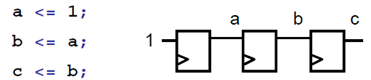
\includegraphics[width=.5\linewidth]{./marco_teorico/FPGA_IP_HDL/img/fpga12}
						\caption{Asignaciones NO bloqueantes en Verilog}
						\label{fig:fpga12}
					\end{figure}
				De esta manera el valor de \emph{c} tarda dos ciclos de reloj en tener el valor actual de \emph{a}.	
				
			\subsubsection{Procesos}
			
				\textbf{Uno de los aspectos m�s importantes en Verilog es la posibilidad de ejecutar en 
				paralelo varios procesos.}Cada proceso se ejecuta de forma secuencial, es decir se ejecuta 
				cada l�nea del proceso seg�n su orden de precedencia. Toda la descripci�n secuencial que se 
				quiera realizar en Verilog debe hacerse dentro de un proceso initial o always. La diferencia 
				entre ambos es que el primero se ejecuta una �nica vez y no es sintetizable, a diferencia del 
				always que se ejecuta cada vez que su lista de sensibilidad lo indique y si es sintetizable 
				en hardware.\\
				La lista de sensibilidad contiene todos los eventos por los que se debe ejecutar las 
				sentencias que contiene el proceso. A continuaci�n se muestra un ejemplo.
				\begin{lstlisting}
always@(/*lista de sensibilidad*/)
	begin
		/*Sentencias Secuenciales*/
	end
				\end{lstlisting}
							
			\subsubsection{Estructuras de Control}
				
				Verilog dispone de estructuras de control, similares a las disponibles en otros lenguajes de 
				programaci�n. Dentro de ellas las que pueden ser sintetizadas son las siguientes.
				\begin{itemize}
				  	\item \textbf{\emph{if - else}}:
				  		La sentencia condicional \emph{if-else} controla la ejecuci�n de otras. En caso de haber 
						m�ltiples sentencias es necesario hacer uso del bloque \emph{begin-end}. La sintaxis de 
						esta estructura es la siguiente.
				  		\begin{lstlisting}
if(/*expresion*/)
	begin
		/*Sentencias*/
	end
else
	begin
		/*Sentencias*/
	end
						\end{lstlisting}
					\item \textbf{\emph{Case}}:
				  		La sentencia \emph{case} es una instrucci�n de decisi�n m�ltiple, eval�a una expresi�n 
						y en funci�n de su valor ejecutar� las sentencias del caso correspondiente. Si existen 
						varias sentencias se debe usarse \emph{begin y end} para contenerlas. Si no se cubren 
						todos los posibles valores se debe hacer uso del caso por defecto, denominado 
						\emph{default}, el cual se ejecutar� cuando ninguno de los casos anteriores se cumpla. 
						La sintaxis de esta estructura es la siguiente.
				  		\begin{lstlisting}
case(/*expresion*/)
	caso 1:
		begin
			/*Sentencias*/
		end
	caso 2:
		begin
			/*Sentencias*/
		end
	.
	.
	.	
	default:
		begin
			/*Sentencias*/
		end		
endcase
						\end{lstlisting}
					\item \textbf{\emph{for}}:
				  		El bucle \emph{for} es id�ntico a los utilizados en otros lenguajes de programaci�n, 
						como en las estructuras mencionadas anteriormente, si existen varias sentencias se deben 
						incluir dentro del bloque \emph{begin-end}. Su sintaxis es la siguiente.
				  		\begin{lstlisting}
for(/*valor inicial*/ ; /*condicion de finalizacion*/ ; /*incremento*/)
	begin
		/*Sentencias*/
	end
						\end{lstlisting}	
				\end{itemize}
				
 		% Desarrollo
 			\part{Desarrollo}
 				% Desarrollo e Implementaci�n
 					%%%%%%%%%%%%%%%%%%%%%%%%%%%%%%%%%%%%%%%%%%%%%%%%%%%%%%%%%%%%%%%%%%%%%%%%%%%%%%%%%%%%%
%																					%
%	TRABAJO: Proyecto Integrador													%
%																					%
%		Titulo: 	Desarrollo de IP cores con procesamiento de Redes de Petri 		%
%					Temporales para sistemas multicore en FPGA						%
%																					%
%		Autores:	Juli�n Nonino													%
%					Carlos Renzo Pisetta											%
%		Director:	Orlando Micolini												%
%																					%
%	Parte: Desarrollo																%
%	Capitulo: Dise�o e Implementaci�n												%	
%	Archivo: chap_diseno_implementacion.tex											%
%																					%
%%%%%%%%%%%%%%%%%%%%%%%%%%%%%%%%%%%%%%%%%%%%%%%%%%%%%%%%%%%%%%%%%%%%%%%%%%%%%%%%%%%%%

% Path Imagenes: ./desarrollo/diseno_implementacion/img
% Nombre predeterminado imagenes: disenoxx
%	xx es el numero de imagen

\lstset
{	language=Verilog,               % the language of the code
	basicstyle=\footnotesize,       % the size of the fonts that are used for the code
	numbers=left,                   % where to put the line-numbers
	numberstyle=\tiny\color{gray},  % the style that is used for the line-numbers
	stepnumber=1,                   % the step between two line-numbers. If it's 1, each line 
                       				% will be numbered
	numbersep=5pt,                  % how far the line-numbers are from the code
	backgroundcolor=\color{white},  % choose the background color. You must add \usepackage{color}
	showspaces=false,               % show spaces adding particular underscores
	showstringspaces=false,         % underline spaces within strings
	showtabs=false,                 % show tabs within strings adding particular underscores
	frame=none,                 	% adds a frame around the code
	rulecolor=\color{white},        % if not set, the frame-color may be changed on line-breaks within not-black text (e.g. comments (green here))
	tabsize=2,                      % sets default tabsize to 2 spaces
	captionpos=b,                   % sets the caption-position to bottom
	breaklines=true,                % sets automatic line breaking
	breakatwhitespace=false,        % sets if automatic breaks should only happen at whitespace
	%title=\lstname,                % show the filename of files included with \lstinputlisting;
		                            % also try caption instead of title
	keywordstyle=\color{blue},      % keyword style
  	commentstyle=\color{dkgreen},   % comment style
  	stringstyle=\color{mauve},      % string literal style
  	escapeinside={\%*}{*)},         % if you want to add LaTeX within your code
  	morekeywords={*,...},           % if you want to add more keywords to the set
  	deletekeywords={...}            % if you want to delete keywords from the given language
}

\chapter{Dise�o e Implementaci�n}
	\label{chap:chap_diseno_implementacion}

	En esta secci�n se describir� la implementaci�n de un \textbf{\emph{procesador de Petri}}, un \emph{IP-Core}
	que resuelve \emph{Redes de Petri con Arcos Inhibidores} en los que se restringe el disparo de transiciones 
	y \emph{Redes de Petri Temporales} donde se introduce el tiempo como condici�n de ejecuci�n.
	En la primera secci�n de este capitulo, se presentar� la arquitectura general del sistema. 
	En las secciones siguientes se explicar� el dise�o y la implementaci�n del procesador de Redes de 
	Petri dividido en dos partes. En la primera parte, se realizo una refactorizaci�n del trabajo descripto 
	en el trabajo \cite{galliapereyra}. Esta refactorizaci�n se realiz� para utilizar Verilog como HDL 
	en lugar del lenguaje VHDL, esto se realiz� por razones de claridad, y adem�s, para permitir una 
	implementaci�n parametrizable que sea mas apta para el agregado de la funcionalidad de procesamiento de 
	Redes de Petri Temporales. En la segunda etapa del proyecto, se dise�� e implement� un IP core para el 
	procesamiento de \textbf{\emph{Redes de Petri con Tiempo}} y otro para la resoluci�n de 
	\textbf{\emph{Redes de Petri Temporizadas}}.
	
	% Arquitectura general del sistema
		%%%%%%%%%%%%%%%%%%%%%%%%%%%%%%%%%%%%%%%%%%%%%%%%%%%%%%%%%%%%%%%%%%%%%%%%%%%%%%%%
%	TRABAJO: Proyecto Integrador
%		Titulo: 	Desarrollo de IP cores con procesamiento de Redes de Petri 	
%					Temporales para sistemas multicore en FPGA					
%		Autores:	Juli�n Nonino												%					Carlos Renzo Pisetta										%		Director:	Orlando Micolini											
%%%%%%%%%%%%%%%%%%%%%%%%%%%%%%%%%%%%%%%%%%%%%%%%%%%%%%%%%%%%%%%%%%%%%%%%%%%%%%%%

% Path im�genes: ./desarrollo/diseno_implementacion/img
% Nombre predeterminado im�genes: disenoxx
%	xx es el numero de imagen

\section{Arquitectura general del sistema}
	\label{sec:arquitectura_general}

	Al comenzar el trabajo, se creo un esquema para describir la ubicaci�n y la conexi�n del procesador de Petri en un sistema multicore.
	\begin{figure}[ht]
		\centering
		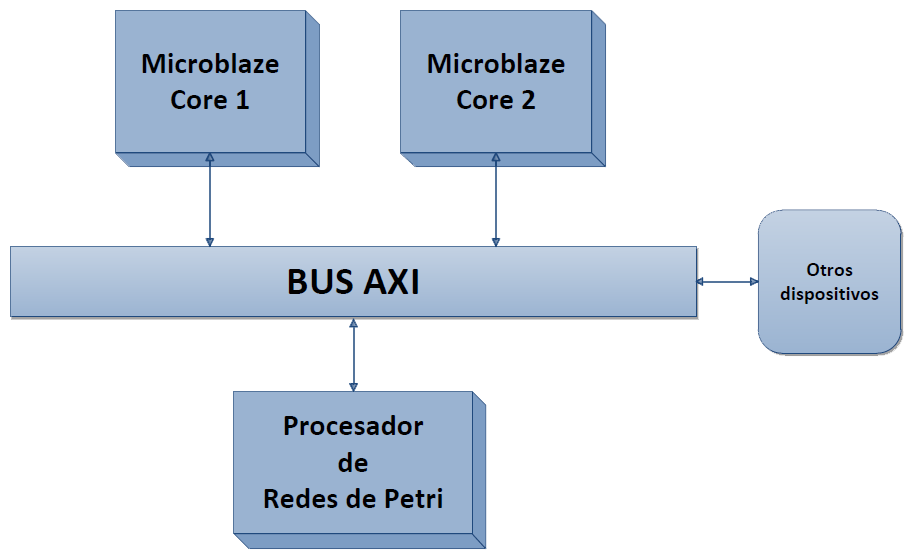
\includegraphics[width=1\linewidth,keepaspectratio]{./desarrollo/diseno_implementacion/img/diseno01}
		\caption{Arquitectura general del sistema}
		\label{fig:diseno01}
	\end{figure}
	
	En el diagrama de la \ref{fig:diseno01}, se observa como esta ubicado el procesador de Petri dentro del sistema. Existen dos cores MicroBlaze de Xilinx que a trav�s del BUS AXI se comunicaran con el procesador de Petri para sincronizarse. Se plante� un sistema con dos procesadores ya que este es el m�nimo numero de cores para que el sistema sea multicore. El procesador de Redes de Petri se encuentra conectado al bus AXI independientemente de los otros procesadores del sistema porque de esta forma, la �nica limitaci�n en el acceso al procesador de Redes de Petri ser�a el bus.
	
	% Procesador de Petri (primera etapa)
		%%%%%%%%%%%%%%%%%%%%%%%%%%%%%%%%%%%%%%%%%%%%%%%%%%%%%%%%%%%%%%%%%%%%%%%%%%%%%%%%
%	TRABAJO: Proyecto Integrador
%		Titulo: 	Desarrollo de IP cores con procesamiento de Redes de Petri 	
%					Temporales para sistemas multicore en FPGA					
%		Autores:	Juli�n Nonino												%					Carlos Renzo Pisetta										%		Director:	Orlando Micolini											
%%%%%%%%%%%%%%%%%%%%%%%%%%%%%%%%%%%%%%%%%%%%%%%%%%%%%%%%%%%%%%%%%%%%%%%%%%%%%%%%

% Path im�genes: ./desarrollo/diseno_implementacion/img
% Nombre predeterminado im�genes: disenoxx
%	xx es el numero de imagen

\section{Procesador de Petri (primera etapa)}
	\label{sec:proc_petri_primera_etapa}

	Como se dijo, en esta primera etapa se realiz� una refactorizaci�n de un trabajo anterior. Para ello, se dise�o nuevamente el sistema generando una arquitectura mas modular que permita la adici�n de funcionalidad nueva de manera sencilla y clara. Adem�s, se dise�o pensando en nuevas caracter�sticas.
	
	\subsection{Requerimientos}
		
		Los requerimientos para esta etapa fueron:
		\begin{enumerate}
			\item: Refactorizar el trabajo descripto en \cite{galliapereyra} generando una arquitectura modularizada en Verilog.
			\item: Implementar el procesamiento con plazas acotadas o limitadas.
			\item: Generar la posibilidad de que se disparen transiciones de manera autom�tica al estar sensibilizadas, sin necesidad de esperar un pedido de disparo explicito.
		\end{enumerate}
	
	\subsection{Arquitectura}
		
		A continuaci�n presentamos la arquitectura del primer procesador de Redes de Petri, el cual est� basado en el algoritmo de ejecuci�n de Redes de Petri (descripto en la secci�n \ref{subsec:redes_con_tiempo}) implementado. Y luego, se describe todas sus funcionalidades e interrelaci�n.
		\newpage
			\begin{figure}[ht]
				\centering
				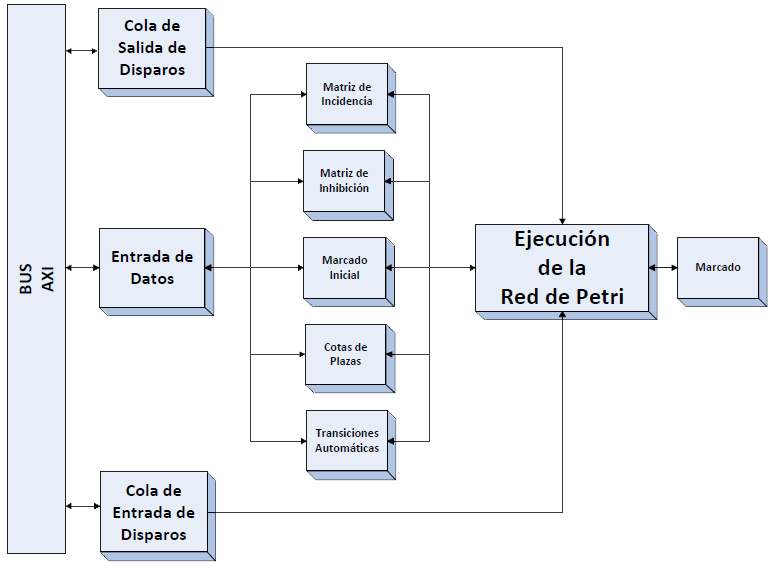
\includegraphics[width=1\linewidth,keepaspectratio]{./desarrollo/diseno_implementacion/img/diseno02}
				\caption{Arquitectura del procesador de Redes de Petri (Primera Parte)}
				\label{fig:diseno02}
			\end{figure}
		
		\subsubsection{Matriz de Incidencia}
			
			La matriz de incidencia, como ya se vio, es una matriz que tiene como cantidad de filas el n�mero de plazas y como cantidad de columnas el n�mero de transiciones. Cada elemento de esta matriz es un n�mero entero con signo.
			\begin{lstlisting}
//Parametros
	parameter cant_plazas			= 15;
	parameter cant_transiciones		= 10;
	parameter tamano_de_elementos	= 6;

//Matriz de incidencia
	reg signed [tamano_de_elementos-1:0] matriz_incidencia [cant_plazas-1:0] [cant_transiciones-1:0];
\end{lstlisting}
		
		\subsubsection{Matriz de inhibici�n}
			
			La matriz de inhibici�n, se declar� de manera similar a la matriz de incidencia. La �nica diferencia con la anterior es que �sta es una matriz binaria. Por lo tanto, cada elemento de esta matriz es de \textbf{un bit}.		
			\begin{lstlisting}
//Matriz de Arcos Inhibidores
	reg matriz_inhibicion [cant_plazas-1:0] [cant_transiciones-1:0];
			\end{lstlisting}

		\subsubsection{Marcado inicial y marcado}
		
			Dado que en Verilog una variable no puede ser modificada en m�s de un \emph{always}, existen dos vectores para almacenar el marcado de la red. Uno llamado \textbf{\emph{marcado inicial}} que es modificado durante la carga de datos. Y, otro llamado \textbf{\emph{marcado}} que es el que almacena el marcado actual de la red y que al comienzo toma el valor que tiene el vector \textbf{\emph{marcado inicial}}.
			\begin{lstlisting}
//Marcado
	reg [tamano_de_elementos-1:0] marcado [cant_plazas-1:0];
	reg [tamano_de_elementos-1:0] marcado_inicial [cant_plazas-1:0];	
			\end{lstlisting}
		
		\subsubsection{Cotas de plazas}
		
			Las cotas en las plazas, se implementan mediante un vector cuya cantidad de elementos es el n�mero de plazas. En realidad, como se esta implementado hardware, todas las plazas est�n limitadas al tama�o de elementos del vector de marcado. Por lo tanto, el vector de cotas, tendr� como tama�o de elementos el mismo que tiene el vector de marcado pudiendo limitar la cantidad de tokens en una plaza desde cero hasta este valor.
			\begin{lstlisting}
//Plazas acotadas
	reg [tamano_de_elementos-2:0] cotas_plazas [cant_plazas-1:0];
			\end{lstlisting}
		
		\subsubsection{Transiciones autom�ticas}
		
			Es un vector binario cuya cantidad de elementos es el n�mero de transiciones. Un \emph{uno} en alg�n elemento indica que la transici�n representada por el mismo es autom�tica y no debe esperar hasta que se solicite su disparo para dispararse, es decir, al momento que se sensibiliza se dispara.		
			\begin{lstlisting}
//Transiciones automaticas
	reg [cant_transiciones-1:0] transiciones_automaticas;
			\end{lstlisting}
		
		\subsubsection{Colas de disparos}
		
			Las colas de disparos son dos, una, para los disparos de entrada que esperan por ser ejecutados en cuanto la red lo permita. Y la otra, para los disparos de salida que ya han sido ejecutados y esperan a que el proceso que solicit� su ejecuci�n los extraiga. La implementaci�n de estas colas se realiza con un contador por cada transici�n que indica cuantos disparos pendientes o ya ejecutados existen para dicha transici�n. Adem�s, existe un vector binario que indica si la cola de una determina transici�n esta vac�a o tiene alg�n valor. Esta implementaci�n obedece a la necesidad de insertar o extraer los disparos en un ciclo de reloj y adem�s, poder contemplar todas las solicitudes de disparos de las distintas transiciones en paralelo.
				\begin{figure}[H]
					\centering
					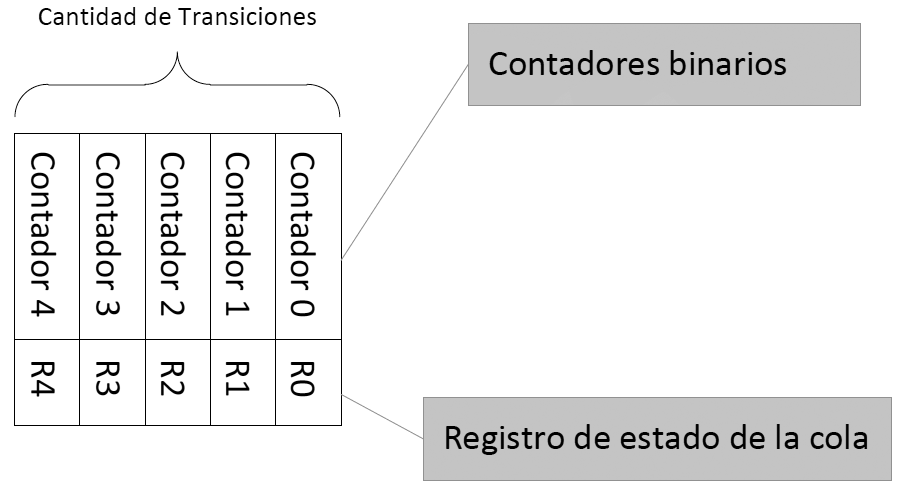
\includegraphics[width=1\linewidth,keepaspectratio]{./desarrollo/diseno_implementacion/img/diseno03}
					\caption{Esquema de las colas de disparos}
					\label{fig:diseno03}
				\end{figure}
			Cada una de las posiciones del vector de estado de la cola indican si esta vac�o o no. Esto se hace de la siguiente manera:
				\begin{figure}[H]
					\centering
					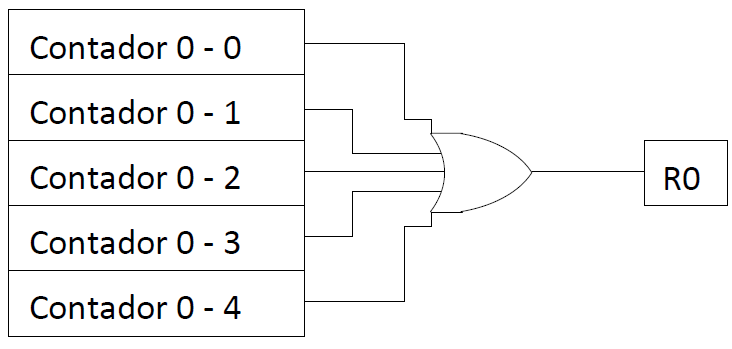
\includegraphics[width=1\linewidth,keepaspectratio]{./desarrollo/diseno_implementacion/img/diseno04}
					\caption{Registro que indica si las colas de disparos est�n vac�as o no}
					\label{fig:diseno04}
				\end{figure}
			Un uno es este vector indica que la cola contiene al menos un elemento. Adem�s, se implementa otro registro de estado que indica si la cola esta llena o no. Este registro se implement� de la siguiente manera. Un uno es este vector indica que la cola esta llena y no puede recibir mas elementos.		
				\begin{figure}[H]
					\centering
					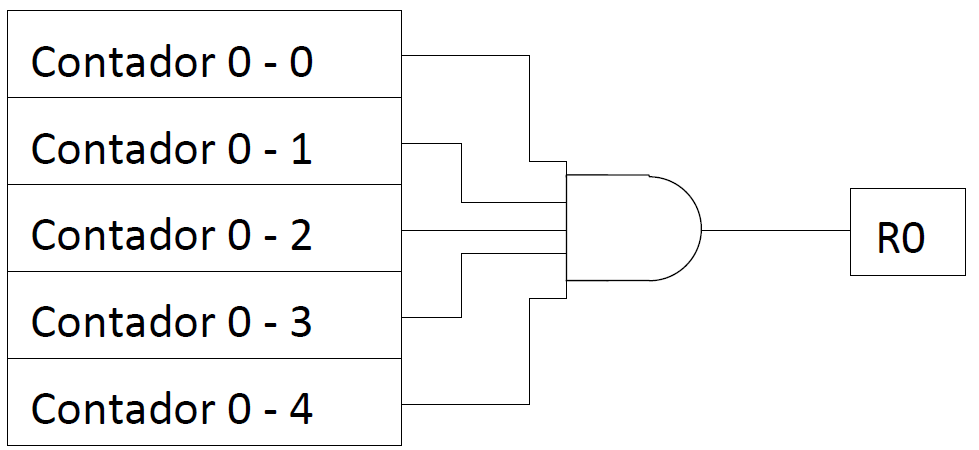
\includegraphics[width=1\linewidth,keepaspectratio]{./desarrollo/diseno_implementacion/img/diseno05}
					\caption{Registro que indica si las colas de disparos est�n llenas o no}
					\label{fig:diseno05}
				\end{figure}
			La implementaci�n de estas colas se realizo en un modulo de Verilog que luego fue instanciado dos veces. Una vez, para la cola de disparos de entrada y otra, para la cola de salida.
			\begin{lstlisting}
/****************************COLA DE ENTRADA DE DISPAROS**********************/
		
	reg [cant_transiciones-1:0] disparo_entrada_incrementa;
	reg [cant_transiciones-1:0] disparo_entrada_decrementa;
	reg [tamano_cola-1:0] counter_cola_disparos_entrada [cant_transiciones-1:0]/* synthesis syn_keep = 1 */;
	integer index_entrada;
	always @(posedge Bus2IP_Clk)
	begin
		if(Bus2IP_Resetn==1'b0)
		begin
			for (index_entrada=0 ; index_entrada<cant_transiciones ; index_entrada=index_entrada+1)
			begin
				counter_cola_disparos_entrada[index_entrada]<={tamano_cola{1'b0}};
			end
		end
		else	
			for (index_entrada=0 ; index_entrada<cant_transiciones ; index_entrada=index_entrada+1)
			begin
				//Incremento cola entrada
					if ({disparo_entrada_incrementa[index_entrada] , disparo_entrada_decrementa[index_entrada]} == 2'b10) //Debe incrementar 
					begin
						counter_cola_disparos_entrada[index_entrada] <= counter_cola_disparos_entrada[index_entrada] + 1'b1;
					end //FIN if(disparo_entrante[index_entrada] == 1'b1)
				//Decremento cola entrada	
					else if ({disparo_entrada_incrementa[index_entrada] , disparo_entrada_decrementa[index_entrada]} == 2'b01) //Debe decrementar  
					begin
						counter_cola_disparos_entrada[index_entrada] <= counter_cola_disparos_entrada[index_entrada] - 1'b1;// {tamano_cola{1'b1}};
					end //FIN if(disparo_dec_entrante[index_entrada] == 1'b1)
				//Otras opciones
					else
					begin
						counter_cola_disparos_entrada[index_entrada] <= counter_cola_disparos_entrada[index_entrada];
					end
			end //FIN for (index_entrada=0 ; index_entrada<cant_transiciones ; index_entrada=index_entrada+1)
	end //FIN always

/****************************COLA DE SALIDA DE DISPAROS**********************/
	reg [tamano_cola-1:0] counter_cola_disparos_salida [cant_transiciones-1:0]/* synthesis syn_keep = 1 */;
	reg [cant_transiciones-1:0] disparo_salida_incrementa;
	reg [cant_transiciones-1:0] disparo_salida_decrementa;
	integer index_salida;
	always @(posedge Bus2IP_Clk)
	begin
		if(Bus2IP_Resetn==1'b0)
		begin
			for (index_salida=0 ; index_salida<cant_transiciones ; index_salida=index_salida+1)
			begin
				counter_cola_disparos_salida[index_salida]<={tamano_cola{1'b0}};
			end
		end
		else	
			for (index_salida=0 ; index_salida<cant_transiciones ; index_salida=index_salida+1)
			begin
				//Incremento cola salida
					if ({disparo_salida_incrementa[index_salida] , disparo_salida_decrementa[index_salida]} == 2'b10) //Debe incrementar 
					begin
						counter_cola_disparos_salida[index_salida] <= counter_cola_disparos_salida[index_salida] + 1'b1;
					end //FIN if(disparo_salida_decrementa[index_salida] == 1'b1)
				//Decremento cola salida	
					else if ({disparo_salida_incrementa[index_salida] , disparo_salida_decrementa[index_salida]} == 2'b01) //Debe decrementar 
					begin
						counter_cola_disparos_salida[index_salida] <= counter_cola_disparos_salida[index_salida] - 1'b1;//{tamano_cola{1'b1}};
					end //FIN if(disparo_salida_decrementa[index_salida] == 1'b1)
				//Otras opciones
					else 
					begin
						counter_cola_disparos_salida[index_salida] <= counter_cola_disparos_salida[index_salida];
					end
			end //FIN for (index_salida=0 ; index_salida<cant_transiciones ; index_salida=index_salida+1)
	end //FIN always
			\end{lstlisting}
		
		\subsubsection{Ejecuci�n de la Red de Petri}
			
			El modulo ejecuci�n de la Red de Petri es el encargado de resolver la ecuaci�n de estado (\ref{eq:ecuacion_estado_uno}) de la red con los disparos que est�n pendientes y realizar la actualizaci�n del marcado en caso de ser necesario. Su funcionamiento ser� explicado en detalle en el apartado \ref{subsec:func_proc_petri}.
		
		\subsubsection{Entrada de datos}
			
			Este modulo es el encargado de cargar todos los datos con los cuales debe operar el Procesador de Redes de Petri para ejecutar la red. Su funcionamiento ser� explicado con detalle en el titulo \ref{subsec:func_proc_petri}.
				
	\subsection{Funcionamiento del procesador de Redes de Petri}
		\label{subsec:func_proc_petri}
		
		En esta secci�n, se presentar�n los diagramas desarrollados con el fin de explicar el funcionamiento del procesador de Redes de Petri mostrando la implementaci�n en Verilog de cada uno de los componentes.
		
		\subsubsection{Carga de datos}
			
			El modulo de carga de datos es el primero que debe entrar en acci�n al utilizar el procesador de Redes de Petri, a trav�s de �l se carga la matriz de incidencia, la matriz de inhibici�n, el marcado inicial, el vector de cotas de plazas y el vector de transiciones autom�ticas.
				\begin{figure}[H]
					\centering
					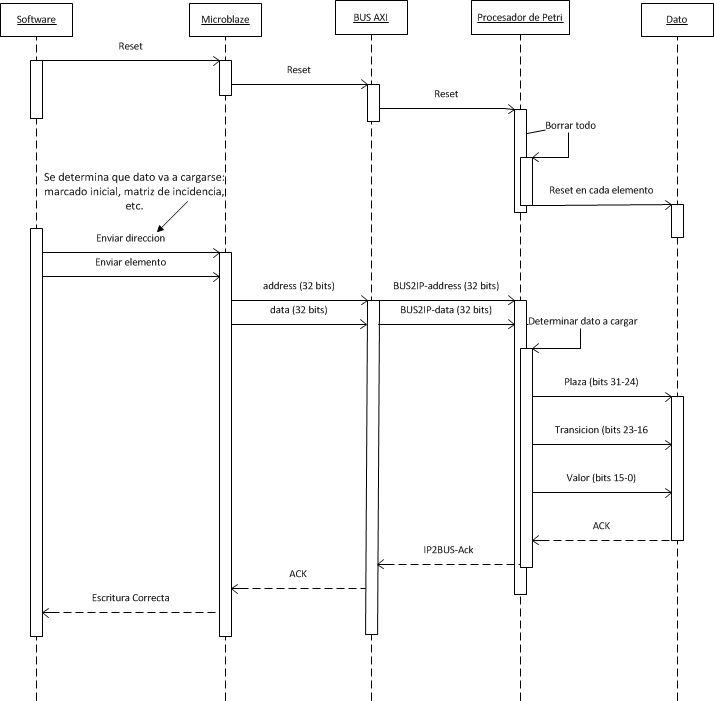
\includegraphics[width=1\linewidth,keepaspectratio]{./desarrollo/diseno_implementacion/img/diseno06}
					\caption{Diagrama de secuencia proceso de carga de datos}
					\label{fig:diseno06}
				\end{figure}
			El software, que se ejecuta en un procesador MicroBlaze desea cargar datos en alguno de los valores representativos de una Red de Petri (matriz de incidencia, marcado inicial, etc.) para programarlo o reprogramarlo. El proceso de carga de datos, se diagram� en la Figura \ref{fig:diseno06} dividido en dos partes. Una secuencia inicial de reset y una secuencia de carga de los elementos que se requieran para programar el funcionamiento del procesador de Petri.
			\\

			\textbf{Secuencia de reset de datos}
				
				La secuencia de reset, se compone de las siguientes etapas.
				\begin{enumerate}
				  	\item El software indica que el procesador MicroBlaze debe ejecutar un reset sobre el procesador de Petri.
				  	\item El procesador MicroBlaze env�a esta orden al procesador de Redes de Petri a trav�s de BUS AXI.
				  	\item El procesador de Redes de Petri procede a borrar todos los valores almacenados poniendo a cero todos los elementos de cada uno de ellos (marcado inicial, matriz de incidencia, etc.)
				\end{enumerate}
		
		
			\textbf{Secuencia de carga de un elemento}	
				
				Se debe aclarar que para la carga de un valor se utiliza una palabra especial de 32 bits, definida de la siguiente manera:
					\begin{figure}[H]
						\centering
						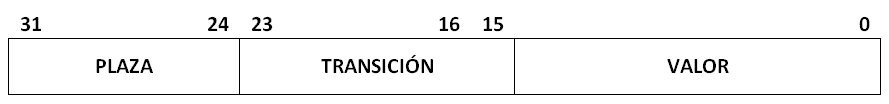
\includegraphics[width=1\linewidth,keepaspectratio]{./desarrollo/diseno_implementacion/img/diseno07}
						\caption{Palabra para la carga de datos en el procesador de Petri}
						\label{fig:diseno07}
					\end{figure}
				
				Esta palabra especial, reserva ocho bits para identificar las plazas y ocho bits para identificar la transici�n. Esto permite una Red de Petri con un m�ximo de 256 plazas y 256 transiciones que se considera tama�o suficiente para la mayor�a de los problemas a resolver. Los restantes 16 bits, identifican el valor que debe ir en el elemento indicado por el n�mero de plaza y por el n�mero de transici�n. Por ejemplo, si se esta cargando la matriz de incidencia y se env�a la siguiente palabra 00000101 00000011 1111111111111101, se cargara en el elemento de la fila 5 y columna 3 el valor -3. Si se carga por ejemplo el marcado inicial, para indicar que la plaza 7 tiene dos tokens al inicio se debe enviar la siguiente palabra 00000111 XXXXXXXX 0000000000000010. Aclarado esto, se explicar� la secuencia de carga.
				
				\begin{enumerate}
				  	\item El software decide cargar un valor, por lo tanto, mediante una direcci�n y un elemento le indica al MicroBlaze lo que debe ejecutar.
				  	\item El MicroBlaze, env�a a trav�s del BUS AXI la palabra de direcci�n y la palabra de dato (address y data).
				  	\item El procesador de Petri identifica que dato se desea cargar mediante la palabra address (si es matriz de incidencia, marcado inicial, etc.). Luego, interpretando la palabra de datos como se mencion� anteriormente, determina que valor se desea escribir y en que posici�n hacerlo.
				  	\item En cada escritura correcta se env�a un ACK para que el software sepa que la operaci�n se realizo con �xito.   
				\end{enumerate}		

		\subsubsection{Llegada de un nuevo disparo por ejecutar}
			
			Cuando llega un nuevo disparo, se utiliza la misma palabra definida en la Figura \ref{fig:diseno07}. Adem�s el procedimiento es bastante similar solo que debe verificarse que la cola de entrada de disparos correspondientes no se encuentre llena.		
				\begin{figure}[H]
					\centering
					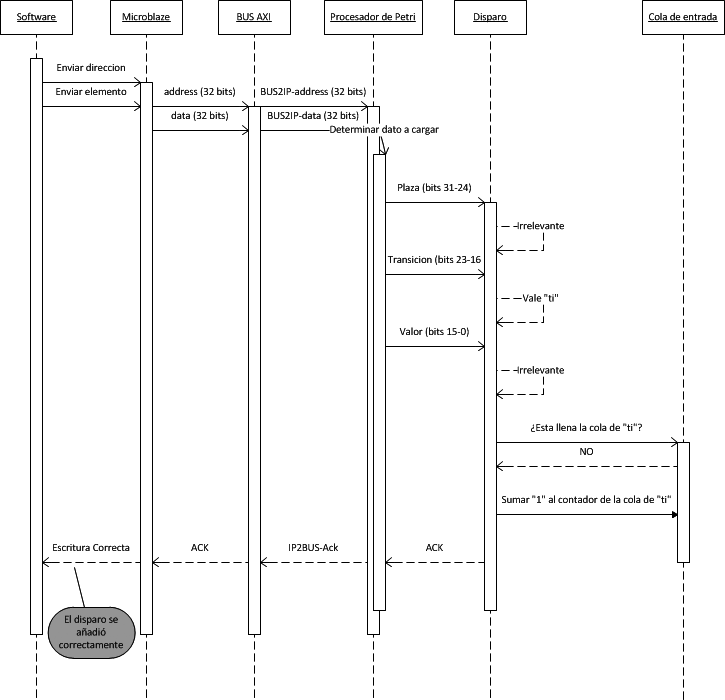
\includegraphics[width=1\linewidth,keepaspectratio]{./desarrollo/diseno_implementacion/img/diseno08}
					\caption{Diagrama de secuencia del ingreso de un nuevo disparo}
					\label{fig:diseno08}
				\end{figure}
			En la secuencia anterior, se observa que el proceso de env�o de un nuevo disparo para que sea ejecutado por el procesador de Redes de Petri es similar al proceso de carga de datos. La diferencia radica en la consulta a la cola acerca de si esta llena o no. Si la cola no esta llena, el disparo es a�adido a la cola y queda a la espera de ser ejecutado. En la Figura \ref{fig:diseno08} no se muestra el caso de que la cola si este llena. Lo que sucede en este caso no se a�ade el disparo a la cola y no se env�a el ACK. De esta manera, el software sabe que la escritura no fue correcta, es decir, el disparo no fue a�adido a la cola.
			
		\subsubsection{Algoritmo de ejecuci�n de Redes de Petri}		
			
			El algoritmo de ejecuci�n de Redes de Petri consiste en detectar los disparos que sean posibles de ser ejecutados y en caso de serlo, resolver la ecuaci�n de estado de la red para lograr un nuevo marcado de la misma. Recordado, la ecuaci�n de estado de una Red de Petri con Arcos Inhibidores \ref{eq:estado_petri_arcos_inhibidores}, tiene la siguiente forma:
				\begin{equation}
					m_{i+1}=m_i+I�[\delta\; and\; f_H(m_i,\;\delta)]
				\end{equation}
			
			La Figura \ref{fig:diseno09} ilustra como se ha implementado la resoluci�n de la ecuaci�n anterior determinando que transiciones est�n sensibilizadas y de acuerdo con los disparos en las colas o aquellas transiciones que son autom�ticas. 
				\begin{figure}[ht]
					\centering
					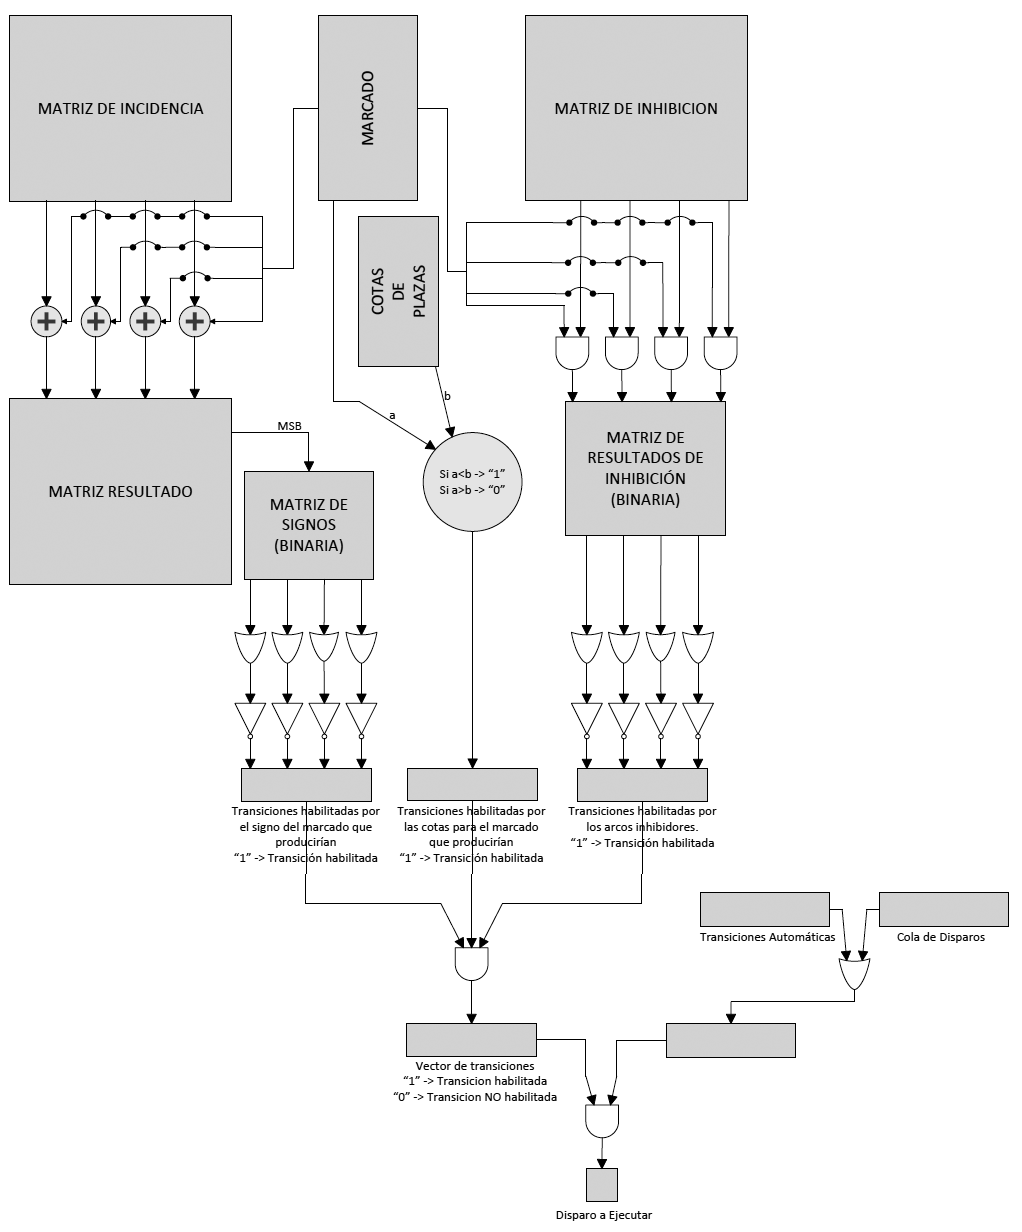
\includegraphics[width=1\linewidth,keepaspectratio]{./desarrollo/diseno_implementacion/img/diseno09}
					\caption{Implementaci�n del Procesador de Redes de Petri}
					\label{fig:diseno09}
				\end{figure}
			
			La matriz de incidencia tiene \emph{P} filas y \emph{T} columnas (\emph{P} es el numero de plazas y \emph{T} es el numero de columnas). Al disparar una transici�n \emph{$t_i$} lo que sucede es que la columna \emph{i} de la matriz se suma con el vector de marcado actual determinando el nuevo marcado. Esto se debe a que los disparos son simples, ejecutan una �nica transici�n. Por esta raz�n, un vector de disparo es un vector con todos sus elementos igual a cero exceptuando que corresponde con la transici�n que desea dispararse. Esto hace que la multiplicaci�n entre la matriz de incidencia y el vector de disparo se transforme una simple selecci�n de columna de la matriz. Esto reduce notablemente la complejidad del hardware.
				
			Dado que existen \emph{T} transiciones, en este procesador de Redes de Petri, se arma una nueva matriz llamada \textbf{\emph{Matriz Resultado}}. Cada columna \emph{k} de esta nueva matriz resulta de sumar la columna \emph{k} de la matriz de incidencia con el vector de marcado. De esta manera, cada columna de la Matriz Resultado es un posible nuevo marcado. Una vez obtenida esta matriz de resultados, se deben detectar valores negativos, cada columna de la matriz representa un posible nuevo marcado y como tal, no debe tener elementos negativos dado que esto indicar�a una cantidad negativa de tokens en una plaza. Para ello, se construye una nueva matriz binaria; cada elemento de esta matriz se corresponde con el bit m�s significativo del elemento de la matriz de resultados. Esta matriz se llama \textbf{\emph{Matriz de Signo}}.
				
			Al mismo tiempo, el vector marcado es operado con la matriz de inhibici�n para determinar si alguna transici�n deja de estar sensibilizada a causa de un arco inhibidor. Como lo determina la ecuaci�n, se realiza una operaci�n \emph{AND} entre el vector de marcado y cada columna de la matriz de inhibici�n. De aqu� surge una nueva matriz, la \textbf{\emph{Matriz de Resultados de Inhibici�n}}, que almacena los resultados de la operaci�n \emph{AND} antes descripta.

			De manera similar, comparando cada elemento del marcado con cada elemento del vector de cotas de plazas, se forma una tercera matriz, \textbf{\emph{matriz de resultados de cotas}}. Esta matriz, tendr� un \emph{1} en el elemento \emph{$a_{ij}$}, significar�a que el posible nuevo marcado que generar�a la transici�n \emph{$t_{j}$} sobre la plaza \emph{$p_{i}$} no superar�a la cota impuesta para esa plaza. 
			\clearpage
			\begin{lstlisting}	
/*****DETERMINACION DE LOS NUEVOS POSIBLES ESTADOS*****/

	//Determinacion de la matriz "resultado".	
	integer columnas;
	integer filas;
	always @(posedge Bus2IP_Clk)
	begin
		for (columnas=0 ; columnas<cant_transiciones ; columnas=columnas+1) //Recorro columnas
		begin
			for (filas=0 ; filas<cant_plazas ; filas=filas+1) // Recorro filas
			begin
				resultado[filas][columnas] = marcado[filas] + matriz_incidencia[filas][columnas]; //Ecuacion
				// Verificacion habilitacion por signo - Creaci�n de matriz
					sign_matrix [columnas][filas] = resultado[filas][columnas][tamano_de_elementos-1];
				//Verificacion habilitacion por inhibicion - Creaci�n de matriz
					inhibe_matrix [columnas][filas] = (|marcado[filas]) & matriz_inhibicion[filas][columnas];
				// Verificacion de habilitacion por cotas - Creaci�n de matriz
					if (resultado[filas][columnas][tamano_de_elementos-1]==1'b0 && resultado[filas][columnas] > cotas_plazas[filas]) // Verifico si supero la cota
					begin
						limit_matrix [columnas][filas] = 1'b0; // Cota SI superada
					end
					else  limit_matrix [columnas][filas] = 1'b1; // Cota NO superada 
			end //Fin for recorre filas
		end //Fin for recorre columnas
	end	
			\end{lstlisting}

			Con estas matrices generadas, se arman tres vectores, el vector de habilitaci�n por signo, el vector de habilitaci�n por inhibici�n y el vector de habilitaci�n por cotas. El \textbf{\emph{vector de habilitaci�n por signo}}, se forma a partir de una \emph{NOR} entre todos los elementos de cada columna de la \emph{Matriz de Signo}. Dado que cada elemento de la matriz de signo es el bit de signo del elemento correspondiente en la matriz de resultado, un valor \emph{1} indicar�a que ese elemento es negativo. Luego, la operaci�n \emph{NOR} detectar�a si en esa columna existe uno o m�s valores negativos. De esta manera, resulta un vector cuya cantidad de elementos es el numero de transiciones y un \emph{1} en el elemento \emph{i} indicar�a que la transici�n \emph{$t_i$} producir�a un marcado sin valores negativos.
			\begin{lstlisting}
for (columnas_habilitaciones=0 ; columnas_habilitaciones<cant_transiciones ; columnas_habilitaciones=columnas_habilitaciones+1) //Recorro columnas
begin
	/*SIGNO*/
	//Determinacion del vector de habilitacion de transiciones segun el "signo"
	t_enable_sign [columnas_habilitaciones] = ~(|(sign_matrix[columnas_habilitaciones][cant_plazas-1:0]));
end
			\end{lstlisting}	

			De manera similar, una operaci�n \emph{NOR} sobre cada columna de la \emph{matriz de resultados de inhibici�n} forma el \textbf{\emph{vector de habilitaci�n por inhibici�n}}. Un valor \emph{1} en el elemento \emph{$a{ij}$} de la \emph{matriz de resultados de inhibici�n} indicar�a que la plaza \emph{$p_i$} contiene elementos y esta unida con un arco inhibidor a la transici�n \emph{$t_j$}. Por lo tanto, esta ultima transici�n no esta sensibilizada. El vector de habilitaci�n por inhibici�n tendr� un \emph{1} en el elemento \emph{j} si es que la transici�n \emph{$t_j$} esta sensibilizada de acuerdo a los arcos inhibidores.
			\begin{lstlisting}
for (columnas_habilitaciones=0 ; columnas_habilitaciones<cant_transiciones ; columnas_habilitaciones=columnas_habilitaciones+1) //Recorro columnas
begin
	/*ARCOS INHIBIDORES*/
	//Determinacion del vector de habilitacion de transicones segun los "arcos inhibidores"
	t_enable_inhibicion [columnas_habilitaciones] = ~(|(inhibe_matrix[columnas_habilitaciones][cant_plazas-1:0]));
end
			\end{lstlisting}
				
			Aplicando una operaci�n \emph{OR} sobre todos los elementos de cada columna de la \emph{matriz de resultados de cotas}, se forma el \textbf{\emph{vector de habilitaci�n por cotas}} en el cual un \emph{1} en el elemento \emph{j} indica que la transici�n \emph{$t_j$} esta sensibilizada seg�n las cotas de plazas.	
			\begin{lstlisting}
for (columnas_habilitaciones=0 ; columnas_habilitaciones<cant_transiciones ; columnas_habilitaciones=columnas_habilitaciones+1) //Recorro columnas
begin
	/*COTAS*/
	//Determinacion del vector de habilitacion de transicones segun las "cotas de plazas"
	t_enable_limit [columnas_habilitaciones] = &(limit_matrix[columnas_habilitaciones][cant_plazas-1:0]);
end
			\end{lstlisting}	

			Los tres vectores de habilitaci�n de transiciones antes mencionados generan a trav�s de una operaci�n \emph{AND} el \textbf{\emph{vector de transiciones sensibilizadas}}. De esta manera, a cada cambio en el marcado de la Red de Petri se determinan cuales son las transiciones sensibilizadas. Esta informaci�n es comparada con la cola de disparos que esperan ser ejecutados y en caso de haber coincidencia, se procede a la ejecuci�n del disparo solicitado.	
			\begin{lstlisting}	
//Determinacion de las transciones habilitadas, disparos posibles
t_sensibilizadas=t_enable_sign & t_enable_inhibicion & t_enable_limit;
			\end{lstlisting}
					
			Obtenido el vector de transiciones sensibilizadas, como lo indica la Figura \ref{fig:diseno09} de la p�gina \pageref{fig:diseno09}, se verifica si el disparo de alguna de �stas transiciones est� solicitado (se encuentra en la cola de entrada de disparos) o, si la transici�n es autom�tica y no se necesita una solicitud para ejecutar su disparo.

			La ejecuci�n de un disparo consiste en actualizar el vector de marcado de la red con la columna correspondiente de la matriz de resultado. Adem�s, el disparo que se ha ejecutado se carga en la cola de disparos de salida y espera ser retirado.
		
		\subsubsection{Retiro de un disparo ejecutado}		
			
			El retiro de un disparo que ya ha sido ejecutado requiere de dos pasos, un proceso que solicito que se dispare una transici�n, debe consultar si el disparo ya se ejecuto y posteriormente, en caso afirmativo, debe remover este disparo de la cola. Para este proceso se pens� en utilizar el mismo sistema que cuando se desea cargar un nuevo disparo en la cola de entrada.
				
				\begin{figure}[ht]
					\centering
					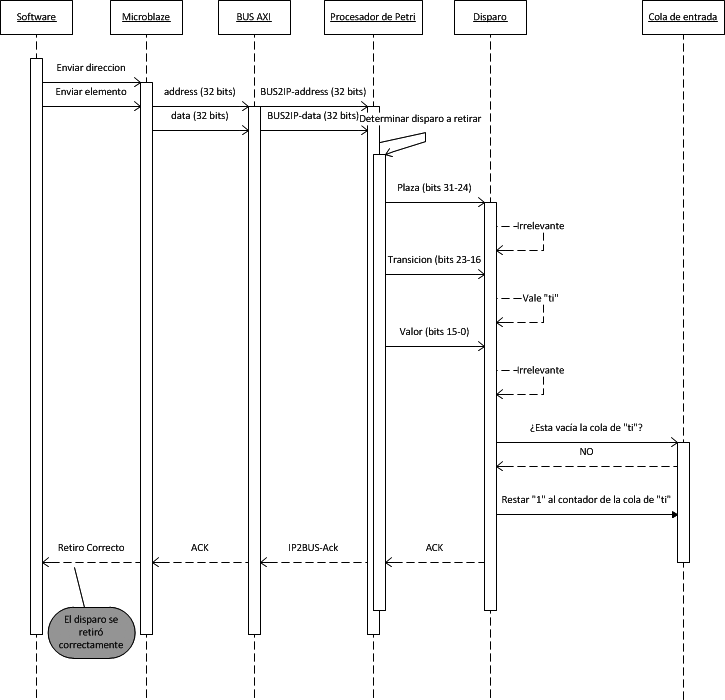
\includegraphics[width=1\linewidth,keepaspectratio]{./desarrollo/diseno_implementacion/img/diseno10}
					\caption{Diagrama de secuencia del retiro de un disparo de la cola de salida}
					\label{fig:diseno10}
				\end{figure}
				
			Se utiliza la palabra definida en la Figura \ref{fig:diseno07} al igual que en el proceso de carga de datos y de llegada de nuevos disparos. En esta palabra de 32 bits, el proceso indica sobre que transici�n desea consultar su ejecuci�n y el retiro de la cola de disparos de salida. Adem�s, esta palabra se acompa�a con una direcci�n que indica que lo que se desea realizar es el retiro de un disparo. Cuando el procesador reconoce la direcci�n y la palabra necesaria para esta operaci�n, consulta la cola del disparo solicitado. Si la cola contiene disparos que esperan salir, se decrementa un unidad (retira un disparo) y se env�a un ACK indicando al software que el disparo hab�a sido ejecutado y que adem�s, fue retirado de la cola. Si el software NO recibe el ACK entiende que su disparo no ha sido ejecutado aun debe consultar nuevamente mas tarde.
				
	\subsection{Verificaci�n}
		
		Para la verificaci�n del funcionamiento de esta primera etapa se ha dise�ado e implementado una prueba en Verilog. En esta prueba se realiza la carga de una Red de Petri simple y sencilla y luego solicita una serie de disparos verificando que la red responda de manera correcta.
			\begin{figure}[H]
				\centering
				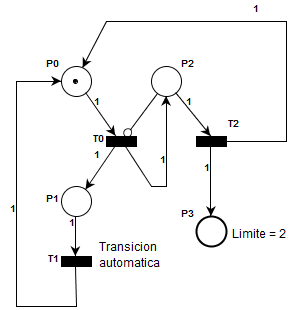
\includegraphics[width=0.5\linewidth,keepaspectratio]{./desarrollo/diseno_implementacion/img/diseno11}
				\caption{Red de Petri para la verificaci�n de la primera etapa de desarrollo}
				\label{fig:diseno11}
			\end{figure}
		
		La red de la \ref{fig:diseno11} ha sido dise�ada solo para que cumpla con ciertas propiedades necesarias para comprobar el correcto funcionamiento del procesador de Redes de Petri. Estas propiedades son:
			\begin{itemize}
			  \item Utilizar arcos inhibidores.
			  \item Tener transiciones autom�ticas.
			  \item Tener plazas con l�mites en la cantidad de tokens.
			  \item Que en alg�n momento varias transiciones est�n sensibilizadas simult�neamente.
			\end{itemize}			
				
		\subsubsection{Carga de datos}
		
			Lo primero que se debe realizar es la carga de los datos necesarios en el procesador. En el test de carga de datos, se utilizan una serie de par�metros para representar las direcciones de cada estructura.		

			\begin{lstlisting}
localparam m_incidencia=32'b00000000000000000000000000000001;
localparam m_inhibicion=32'b00000000000000000000000000000010;
localparam m_marcado=32'b00000000000000000000000000000100;
localparam p_cotas=32'b00000000000000000000000000001000;
localparam t_automatica=32'b00000000000000000000000000010000;
localparam new_disparo=32'b00000000000000000000000000100000;
localparam sacardisparo=32'b00000000000000000000000001000000;
localparam error=32'b00000000000000000000000000000111;
			\end{lstlisting}
			
			\begin{itemize}
			  	\item \emph{Carga del vector de marcado inicial:}
			  		El vector de marcado inicial, tiene la siguiente forma:
			  		\begin{equation}
			  			m_0 = \begin{bmatrix}
			  					1 \\
			  					0 \\
			  					0 \\
			  					0
			  				\end{bmatrix}
			  		\end{equation}
			  		La carga de estos valores en el procesador de Redes de Petri se realiza a trav�s del test en Verilog de la siguiente manera:
					\begin{lstlisting}			  		
//Marcado inicial [0]
	@(posedge clk)
	address 	= m_marcado;
	//Plazas: 00000000=00H - Transiciones: 00000000=00H - Elemento: 0000000000000001
	bus_in 	= 32'h00000001;
	#20;
//Marcado inicial [1]
	@(posedge clk)
	address 	= m_marcado;
	//Plazas: 00000001=01H - Transiciones: 00000000=00H - Elemento: 0000000000000000
	bus_in 	= 32'h01000000;	
	#20;
//Marcado inicial [2]
	@(posedge clk)
	address 	= m_marcado;
	//Plazas: 00000010=02H - Transiciones: 00000000=00H - Elemento: 0000000000000000
	bus_in 	= 32'h02000000;	
	#20;
//Marcado inicial [3]
	@(posedge clk)
	address 	= m_marcado;
	//Plazas: 00000011=03H - Transiciones: 00000000=00H - Elemento: 0000000000000000
	bus_in 	= 32'h03000000;	
	#20;
					\end{lstlisting}			  		
			  		
					Recordando los par�metros antes mencionados, en la Figura \ref{fig:diseno12} se encuentra una imagen de la simulaci�n en la cual se pasa el valor \emph{4H} en la entrada \emph{address} (este valor corresponde al marcado inicial). Simult�neamente, se sit�a en el bus el valor a cargar en el primer elemento de vector de marcado inicial.
			  		\begin{figure}[H]
						\centering
						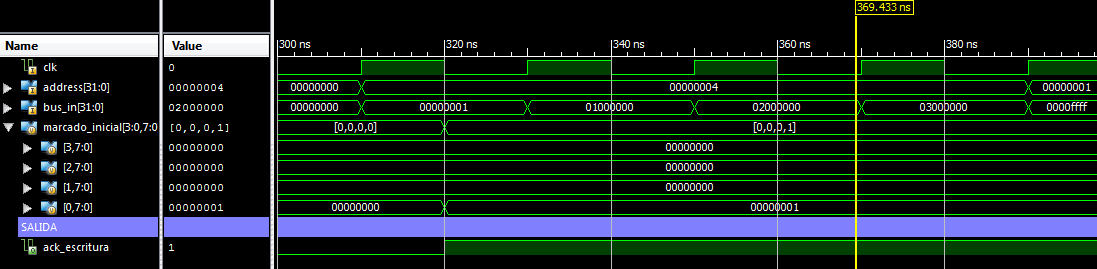
\includegraphics[width=0.9\linewidth,keepaspectratio]{./desarrollo/diseno_implementacion/img/diseno12}
						\caption{Simulaci�n de la carga del vector de marcado inicial}
						\label{fig:diseno12}
					\end{figure}
			  		En la imagen anterior, es posible observar el valor final de vector marcado inicial, notando que coincide con el valor que se deseaba cargar\footnote{La columna \emph{value} de la Figura representa el valor de la variable en el instante marcado por la l�nea amarilla.}. En el momento de la carga del primer elemento del vector de marcado inicial, se puede notar que medio ciclo despu�s de colocar el valor en el bus, se encuentra cargado en la estructura correspondiente.
			  		
			  	\item \emph{Carga de la matriz de incidencia:}
			  		La matriz de incidencia para la Red de Petri de la Figura \ref{fig:diseno11} 
			  		tiene la siguiente forma:
			  		\begin{equation}
			  			I = \begin{bmatrix}
			  					-1 & 1  & 1  \\
			  					1  & -1 & 0  \\
			  					1  & 0  & -1 \\
			  					0  & 0  & 1
			  				\end{bmatrix}
			  		\end{equation}
			  		La carga de estos valores en el procesador de Redes de Petri se realiza a trav�s del test en Verilog de la siguiente manera:
			  		\begin{lstlisting}	
//Matriz de incidencia [0][0]
	@(posedge clk)
	address 	= m_incidencia;
	//Plazas: 00000000=00H - Transiciones: 00000000=00H - Elemento: 1111111111111111
	bus_in 	= 32'h0000FFFF;	
	#20
//Matriz de incidencia [0][1]
	@(posedge clk)
	address 	= m_incidencia;
	//Plazas: 00000000=00H - Transiciones: 00000001=01H - Elemento: 0000000000000001
	bus_in 	= 32'h00010001;	
	#20;
//Matriz de incidencia [0][2]
	@(posedge clk)
	address 	= m_incidencia;
	//Plazas: 00000000=00H - Transiciones: 00000010=02H - Elemento: 0000000000000001
	bus_in 	= 32'h00020001;
	#20;	
//Matriz de incidencia [1][0]
	@(posedge clk)
	address 	= m_incidencia;
	//Plazas: 00000001=01H - Transiciones: 00000000=00H - Elemento: 0000000000000001
	bus_in 	= 32'h01000001;	
	#20;
//Matriz de incidencia [1][1]
	@(posedge clk)
	address 	= m_incidencia;
	//Plazas: 00000001=01H - Transiciones: 00000001=01H - Elemento: 1111111111111111
	bus_in 	= 32'h0101FFFF;	
	#20;
//Matriz de incidencia [1][2]
	@(posedge clk)
	address 	= m_incidencia;
	//Plazas: 00000001=01H - Transiciones: 00000010=02H - Elemento: 0000000000000000
	bus_in 	= 32'h01020000;	
	#20;
//Matriz de incidencia [2][0]
	@(posedge clk)
	address 	= m_incidencia;
	//Plazas: 00000010=02H - Transiciones: 00000000=00H - Elemento: 0000000000000001
	bus_in 	= 32'h02000001;	
	#20;
//Matriz de incidencia [2][1]
	@(posedge clk)
	address 	= m_incidencia;
	//Plazas: 00000010=02H - Transiciones: 00000001=01H - Elemento: 0000000000000000
	bus_in 	= 32'h02010000;	
	#20;
//Matriz de incidencia [2][2]
	@(posedge clk)
	address 	= m_incidencia;
	//Plazas: 00000010=02H - Transiciones: 00000010=02H - Elemento: 1111111111111111
	bus_in 	= 32'h0202FFFF;	
	#20;	
//Matriz de incidencia [3][0]
	@(posedge clk)
	address 	= m_incidencia;
	//Plazas: 00000011=03H - Transiciones: 00000000=00H - Elemento: 0000000000000000
	bus_in 	= 32'h03000000;	
	#20;
//Matriz de incidencia [3][1]
	@(posedge clk)
	address 	= m_incidencia;
	//Plazas: 00000011=03H - Transiciones: 00000001=01H - Elemento: 0000000000000000
	bus_in 	= 32'h03010000;	
	#20;
//Matriz de incidencia [3][2]
	@(posedge clk)
	address 	= m_incidencia;
	//Plazas: 00000011=03H - Transiciones: 00000010=02H - Elemento: 0000000000000001
	bus_in 	= 32'h03020001;	
	#20;
					\end{lstlisting}
			  		
					La siguiente imagen, mostrara que la matriz de incidencia a sido efectivamente cargada.	
					\begin{figure}[H]
						\centering
						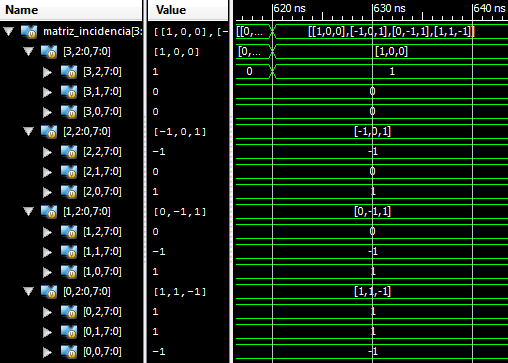
\includegraphics[width=0.6\linewidth,keepaspectratio]{./desarrollo/diseno_implementacion/img/diseno13}
						\caption{Valor que alcanza la matriz de incidencia luego del proceso de carga}
						\label{fig:diseno13}
					\end{figure}
					
				\item \emph{Carga de la matriz de inhibici�n}
					La matriz de arcos inhibidores resulta:		  		
			  		\begin{equation}
			  			H = \begin{bmatrix}
			  					0 & 0 & 0 \\
			  					0 & 0 & 0 \\
			  					1 & 0 & 0 \\
			  					0 & 0 & 0
			  				\end{bmatrix}
			  		\end{equation}
			  		La carga de estos valores en el procesador de Redes de Petri se realiza a trav�s del test en Verilog de la siguiente manera:
			  		\begin{lstlisting}	
//Matriz de inhibicion [0][0]
	@(posedge clk)
	address 	= m_inhibicion;
	//Plazas: 00000000=00H - Transiciones: 00000000=00H - Elemento: 0000000000000000
	bus_in 	= 32'h00000000;	
	#20;
//Matriz de inhibicion [0][1]
	@(posedge clk)
	address 	= m_inhibicion;
	//Plazas: 00000000=00H - Transiciones: 00000001=01H - Elemento: 0000000000000000
	bus_in 	= 32'h00010000;	
	#20;
//Matriz de inhibicion [0][2]
	@(posedge clk)
	address 	= m_inhibicion;
	//Plazas: 00000000=00H - Transiciones: 00000010=02H - Elemento: 0000000000000000
	bus_in 	= 32'h00020000;	
	#20;	
//Matriz de inhibicion [1][0]
	@(posedge clk)
	address 	= m_inhibicion;
	//Plazas: 00000001=01H - Transiciones: 00000000=00H - Elemento: 0000000000000000
	bus_in 	= 32'h01000000;	
	#20;
//Matriz de inhibicion [1][1]
	@(posedge clk)
	address 	= m_inhibicion;
	//Plazas: 00000001=01H - Transiciones: 00000001=01H - Elemento: 0000000000000000
	bus_in 	= 32'h01010000;	
	#20;
//Matriz de inhibicion [1][2]
	@(posedge clk)
	address 	= m_inhibicion;
	//Plazas: 00000001=01H - Transiciones: 00000010=02H - Elemento: 0000000000000000
	bus_in 	= 32'h01020000;	
	#20;	
//Matriz de inhibicion [2][0]
	@(posedge clk)
	address 	= m_inhibicion;
	//Plazas: 00000010=02H - Transiciones: 00000000=00H - Elemento: 0000000000000001
	bus_in 	= 32'h02000001;	
	#20;
//Matriz de inhibicion [2][1]
	@(posedge clk)
	address 	= m_inhibicion;
	//Plazas: 00000010=02H - Transiciones: 00000001=01H - Elemento: 0000000000000000
	bus_in 	= 32'h02010000;	
	#20;
//Matriz de inhibicion [2][2]
	@(posedge clk)
	address 	= m_inhibicion;
	//Plazas: 00000010=02H - Transiciones: 00000010=02H - Elemento: 0000000000000000
	bus_in 	= 32'h02020000;	
	#20;	
//Matriz de inhibicion [3][0]
	@(posedge clk)
	address 	= m_inhibicion;
	//Plazas: 00000011=03H - Transiciones: 00000000=00H - Elemento: 0000000000000000
	bus_in 	= 32'h03000001;	
	#20;
//Matriz de inhibicion [3][1]
	@(posedge clk)
	address 	= m_inhibicion;
	//Plazas: 00000011=03H - Transiciones: 00000001=01H - Elemento: 0000000000000000
	bus_in 	= 32'h03010000;	
	#20;
//Matriz de inhibicion [3][2]
	@(posedge clk)
	address 	= m_inhibicion;
	//Plazas: 00000011=03H - Transiciones: 00000010=02H - Elemento: 0000000000000000
	bus_in 	= 32'h03020000;	
	#20;
					\end{lstlisting}
					De manera similar al caso anterior, se ver� como resulta la matriz de inhibici�n:
					\begin{figure}[H]
						\centering
						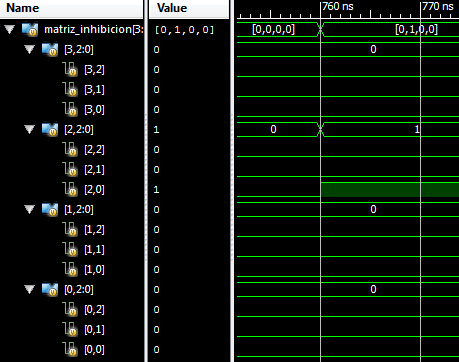
\includegraphics[width=0.7\linewidth,keepaspectratio]{./desarrollo/diseno_implementacion/img/diseno14}
						\caption{Valor que alcanza la matriz de inhibici�n luego del proceso de carga}
						\label{fig:diseno14}
					\end{figure}
				
				\item \emph{Carga del vector de cotas en plazas}	
					El vector de cotas de plazas es:
					\begin{equation}
			  			\begin{bmatrix}
			  				P_0 \\
			  				P_2 \\
			  				P_2 \\
			  				P_3 
			  			\end{bmatrix} 
			  			=
			  			\begin{bmatrix}
			  				max \\
			  				max \\
			  				max \\
			  				2 	
			  			\end{bmatrix} 
			  		\end{equation}
					La carga de estos valores en el procesador de Redes de Petri se realiza a trav�s del test en Verilog de la siguiente manera:
					\begin{lstlisting}
//Vector de cotas [0]
	@(posedge clk)
	address 	= p_cotas;
	//Plazas: 00000000=00H - Transiciones: 00000000=00H - Elemento: 1111111111111111
	bus_in	= 32'h0000FFFF;	
	#20;
//Vector de cotas [1]
	@(posedge clk)
	address 	= p_cotas;
	//Plazas: 00000001=01H - Transiciones: 00000000=00H - Elemento: 1111111111111111
	bus_in	= 32'h0100FFFF;	
	#20;
//Vector de cotas [2]
	@(posedge clk)
	address 	= p_cotas;
	//Plazas: 00000010=02H - Transiciones: 00000000=00H - Elemento: 1111111111111111
	bus_in	= 32'h0200FFFF;	
	#20;
//Vector de cotas [3]
	@(posedge clk)
	address 	= p_cotas;
	//Plazas: 00000011=03H - Transiciones: 00000000=00H - Elemento: 0000000000000010
	bus_in	= 32'h03000002;	
	#20;
					\end{lstlisting}
					
					En la simulaci�n observamos lo siguiente:
					\begin{figure}[H]
						\centering
						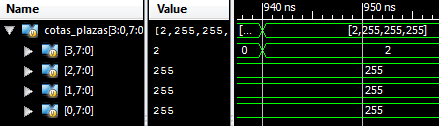
\includegraphics[width=0.55\linewidth,keepaspectratio]{./desarrollo/diseno_implementacion/img/diseno15}
						\caption{Valor que alcanza el vector de cotas de plazas luego del proceso de carga}
						\label{fig:diseno15}
					\end{figure}
				
				\item \emph{Carga del vector de transiciones autom�ticas}	
					El vector de transiciones autom�ticas tiene la siguiente forma:
					\begin{equation}
			  			\begin{bmatrix}
			  				T_0 \\
			  				T_2 \\
			  				T_2
			  			\end{bmatrix} 
			  			=
			  			\begin{bmatrix}
			  				0 \\
			  				1 \\
			  				0
			  			\end{bmatrix} 
			  		\end{equation}
			  		La carga de estos valores en el procesador de Redes de Petri se realiza a trav�s del test en Verilog de la siguiente manera:
			  		\begin{lstlisting}
//Transicion Automatica [0]
	@(posedge clk)
	address 	= t_automatica;
	//Plazas: 00000000=00H - Transiciones: 00000000=00H - Elemento: 0000000000000000
	bus_in	= 32'h00000000;	
	#20;
//Transicion Automatica[1]
	@(posedge clk)
	address 	= t_automatica;
	//Plazas: 00000000=01H - Transiciones: 00000001=01H - Elemento: 0000000000000001
	bus_in	= 32'h00010001;	
	#20;
//Transicion Automatica[2]
	@(posedge clk)
	address 	= t_automatica;
	//Plazas: 00000000=01H - Transiciones: 00000010=02H - Elemento: 0000000000000000
	bus_in	= 32'h00020000;	
	#20;
					\end{lstlisting}
					Observando como resulta este vector en la simulaci�n:
					\begin{figure}[H]
						\centering
						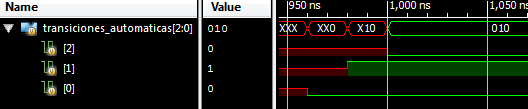
\includegraphics[width=0.55\linewidth,keepaspectratio]{./desarrollo/diseno_implementacion/img/diseno16}
						\caption{Valor que alcanza el vector de transiciones autom�ticas luego del proceso de carga}
						\label{fig:diseno16}
					\end{figure}			  		
			\end{itemize}
	
		\subsubsection{Secuencia de disparos}
			
			A continuaci�n, se presentar� la secuencia de disparos que se aplicar� sobre la Red de Petri de la \ref{fig:diseno11}. Cada disparo que se aplique, producir� un marcado que se comparara con el obtenido en un simulador de Redes de Petri (PIPE versi�n 4).
			\begin{center}
				$S = { T2, T0, T0, T0, T2, T0 }$
			\end{center}
			Se debe notar que la transici�n \emph{T1} no se encuentra incluida en la lista debido a que fue marcada como autom�tica, por lo tanto, no es necesario hacer un pedido para que sea disparada. La secuencia de disparos ha sido elegida con el fin de que se compruebe el comportamiento del procesador de Redes de Petri en diversas circunstancias. La Figura \ref{fig:diseno16} muestra la simulaci�n del �ltimo dato cargado en el Procesador de Redes de Petri. Como se observa en dicha Figura, en el instante de los 1000 ns el procesador ya esta listo para comenzar recibir solicitudes de disparos. La afirmaci�n anterior es demostrada por la siguiente Figura (\ref{fig:diseno17}).
				\begin{figure}[H]
					\centering
					\includegraphics[width=0.75\linewidth,keepaspectratio]{./desarrollo/diseno_implementacion/img/diseno17}
					\caption{Estado del Procesador de Redes de Petri luego de la carga de todos los datos}
					\label{fig:diseno17}
				\end{figure}
			Se observa que al comenzar, el procesador de Petri determina que el �nico disparo posible es el de la transici�n \emph{0}, coincidiendo con el simulador.
				\begin{figure}[H]
					\centering
					\includegraphics[width=0.3\linewidth,keepaspectratio]{./desarrollo/diseno_implementacion/img/diseno18}
					\caption{Estado inicial de la Red de Petri}
					\label{fig:diseno18}
				\end{figure}
			Partiendo desde esta situaci�n, se puede comenzar a enviar la secuencia de disparos.
			
			\begin{enumerate}
				\item \emph{Solicitar el disparo de \textbf{T2}}
					
					Esta solicitud se env�a para comprobar que el procesador ubica correctamente en la cola de espera a las solicitudes de disparo para transiciones que no est�n sensibilizadas como es el caso de \emph{T2}.
					\begin{lstlisting}
//Solicito disparo de T2 -> Deber�a ir a la cola porque T2 NO esta sensibilizada
@(posedge clk)
address	= new_disparo;
//Plazas: 00000000=00H - Transiciones: 00000010=02H - Elemento: 0000000000000000
bus_in = 32'h00020000;	
@(negedge clk)
address	= error;
					\end{lstlisting}					
					\begin{figure}[H]
						\centering
						\includegraphics[width=1\linewidth,keepaspectratio]{./desarrollo/diseno_implementacion/img/diseno19}
						\caption{Simulaci�n primer disparo de la secuencia de prueba}
						\label{fig:diseno19}
					\end{figure}
				
					En la Figura \ref{fig:diseno19} la simulaci�n del procesador de Redes de Petri cuando llega la primera solicitud de disparo. Como se dijo, esta solicitud es para una transici�n que no esta sensibilizada por lo tanto, no se encuentra entre los disparos posibles y queda almacenado en la cola.
									
				\item \emph{Solicitar el disparo de \textbf{T0}}
					
					Luego, se solicita el disparo de la transici�n \emph{T0} esperando que sea disparada porque es la �nica transici�n sensibilizada.
					\begin{figure}[H]
						\centering
						\includegraphics[width=0.4\linewidth,keepaspectratio]{./desarrollo/diseno_implementacion/img/diseno20}
						\caption{Estado esperado de la Red luego de disparar \emph{T0}}
						\label{fig:diseno20}
					\end{figure}
					Al solicitar el disparo, se observa que es cargado en la cola. Luego, como el procesador reconoce que es una solicitud sobre una transici�n que esta sensibilizada la ejecuta.					
					\begin{figure}[H]
						\centering
						\includegraphics[width=1\linewidth,keepaspectratio]{./desarrollo/diseno_implementacion/img/diseno21}
						\caption{Solicitud y disparo de la transici�n \emph{T0}}
						\label{fig:diseno21}
					\end{figure}
					La l�nea amarilla marca el instante en el cual se pone en el bus el address correspondiente a un nuevo disparo y el valor que indica que disparo se desea solicitar. Ese nuevo dato, se coloca en el bus en un flanco positivo de reloj, el procesador de Redes de Petri recibe el dato en el flanco negativo. Luego de la recepci�n del disparo se demora un ciclo en colocar el disparo en la cola de entrada correspondiente y un ciclo en actualizar el marcado a partir de un disparo que se encuentre en la cola. 
					
					\textbf{\emph{De esta manera, se observa que cuando llega un nuevo disparo, en dos ciclos el procesador de Redes de Petri genera el cambio de estado.}} Se debe notar que luego de que el marcado cambi�, el procesador necesita medio ciclo para calcular el nuevo vector de disparos posibles.

					Luego de que la transici�n \emph{T0} se dispara, quedan sensibilizadas las transiciones \emph{T1} y \emph{T2}. Como la primera de ellas es una transici�n autom�tica y la segunda fue solicitada anteriormente, ambas se ejecutan y se actualiza el marcado.

					La Figura \ref{fig:diseno22} muestra como, luego de que el marcado fue actualizado por la transici�n \emph{T0}, la transici�n \emph{T2} que se encontraba en la cola de disparos en espera es disparada y luego la transici�n \emph{T1} que fue marcada como autom�tica. Cada uno de estos disparos, como ya estaban las solicitudes dentro del procesador, toma solo un ciclo de ejecuci�n cada uno.

					En la imagen, puede observarse como dejan de ser posibles los disparos \emph{T2} y \emph{T1} y comienza a estar sensibilizada la transici�n \emph{T0}, tambi�n se observa como se marcan estos disparos en la cola de los que ya han sido ejecutados.
					\begin{figure}[H]
						\centering
						\includegraphics[width=0.75\linewidth,keepaspectratio]{./desarrollo/diseno_implementacion/img/diseno22}
						\caption{Disparo de las transiciones \emph{T0} y \emph{T2}}
						\label{fig:diseno22}
					\end{figure}
					
					\begin{figure}[H]
						\centering
						\includegraphics[width=0.75\linewidth,keepaspectratio]{./desarrollo/diseno_implementacion/img/diseno23}
						\caption{Cambios de estado en la Red de Petri}
						\label{fig:diseno23}
					\end{figure}
									
					Comparando la Figura \ref{fig:diseno22} con la Figura \ref{fig:diseno23} se observa coinciden los sucesivos marcados y las transiciones que se encuentran sensibilizadas en cada uno de ellos.
				
				\item \emph{Solicitar el disparo de \textbf{T0}}
					
					\begin{figure}[H]
						\centering
						\includegraphics[width=1\linewidth,keepaspectratio]{./desarrollo/diseno_implementacion/img/diseno24}
						\caption{Segundo disparo de la transici�n \emph{T0} (simulaci�n)}
						\label{fig:diseno24}
					\end{figure}
					
					\begin{figure}[H]
						\centering
						\includegraphics[width=0.5\linewidth,keepaspectratio]{./desarrollo/diseno_implementacion/img/diseno25}
						\caption{Segundo disparo de la transici�n \emph{T0} (Red de Petri)}
						\label{fig:diseno25}
					\end{figure}
					
					Se solicita el disparo de la transici�n \emph{T0} dado que esta sensibilizada. Luego, la transici�n \emph{T1} se disparar� por ser una transici�n autom�tica.
					
					\begin{figure}[H]
						\centering
						\includegraphics[width=1\linewidth,keepaspectratio]{./desarrollo/diseno_implementacion/img/diseno26}
						\caption{Disparo autom�tico de \emph{T1} (simulaci�n)}
						\label{fig:diseno26}
					\end{figure}
					
					\begin{figure}[H]
						\centering
						\includegraphics[width=0.4\linewidth,keepaspectratio]{./desarrollo/diseno_implementacion/img/diseno27}
						\caption{Disparo autom�tico de \emph{T1} (Red de Petri)}
						\label{fig:diseno27}
					\end{figure}
				
					En las Figuras \ref{fig:diseno26} y \ref{fig:diseno27} se observa que tras el disparo autom�tico de \emph{T1}, \emph{T0} no resulta sensibilizada por el arco inhibidor que la une a \emph{P2}.
					
				\item \emph{Solicitar el disparo de \textbf{T0}}
					
					Dado que \emph{T0} no esta sensibilizada por al solicitar su disparo, se almacenara en la cola de espera.
					
					\begin{figure}[H]
						\centering
						\includegraphics[width=1\linewidth,keepaspectratio]{./desarrollo/diseno_implementacion/img/diseno28}
						\caption{Solicitud de disparo de \emph{T0}}
						\label{fig:diseno28}
					\end{figure}
					
					En la Figura \ref{fig:diseno28} se observa como al solicitar el disparo de \emph{T0} queda en la cola de disparos en espera.
									
				\item \emph{Solicitar el disparo de \textbf{T2}}			  
			  
			  		La �nica transici�n sensibilizada en este momento es la transici�n \emph{T2} entonces, al solicitar su disparo se ejecutar�.
			  		
			  		\begin{figure}[H]
						\centering
						\includegraphics[width=0.4\linewidth,keepaspectratio]{./desarrollo/diseno_implementacion/img/diseno29}
						\caption{Disparo de \emph{T2} (Red de Petri)}
						\label{fig:diseno29}
					\end{figure}
			  		
			  		Al disparar la transici�n \emph{T2} la plaza \emph{P3} alcanza una cantidad de dos tokens, dado que estaba limitada a esta cantidad, la transici�n \emph{T2} ya no podr� estar sensibilizada.
			  		
			  		\begin{figure}[H]
						\centering
						\includegraphics[width=1\linewidth,keepaspectratio]{./desarrollo/diseno_implementacion/img/diseno30}
						\caption{Disparo de \emph{T2} (simulaci�n)}
						\label{fig:diseno30}
					\end{figure}
			  		
			  		En la Figura \ref{fig:diseno30}, se observa que el vector \emph{t enable limit} indica que la transici�n \emph{T2} deja de estar sensibilizada por las cotas en las plazas.

					Como el disparo de la transici�n \emph{T0} estaba solicitado y dispararla implica que \emph{T1} quede sensibilizada y por ser autom�tica tambi�n se disparar�.
			  		
			  		\begin{figure}[H]
						\centering
						\includegraphics[width=0.8\linewidth,keepaspectratio]{./desarrollo/diseno_implementacion/img/diseno31}
						\caption{Disparos de \emph{T0} y \emph{T1} (Red de Petri)}
						\label{fig:diseno31}
					\end{figure}
			  		
			  		Tras el disparo de estas transiciones, se observa que \emph{T0} no puede estar sensibilizada debido al arco inhibidor que la une a \emph{P2}. \emph{T1} no puede sensibilizarse porque \emph{P1} no tiene tokens. Y, \emph{T2} no puede sensibilizarse porque \emph{P3} alcanz� su l�mite de tokens. La Red de Petri queda bloqueada.

					\begin{figure}[H]
						\centering
						\includegraphics[width=1\linewidth,keepaspectratio]{./desarrollo/diseno_implementacion/img/diseno32}
						\caption{Disparos de \emph{T0} y \emph{T1} (simulaci�n)}
						\label{fig:diseno32}
					\end{figure}
			  		
			 		Se observa que el bit \textbf{\emph{red activa}} indica que la Red de Petri alcanz� un estado a partir del cual no puede continuar.
			  
			\end{enumerate}
			
		
	% Procesador de Petri (segunda etapa)
		%%%%%%%%%%%%%%%%%%%%%%%%%%%%%%%%%%%%%%%%%%%%%%%%%%%%%%%%%%%%%%%%%%%%%%%%%%%%%%%%%%%%%
%																					%
%	TRABAJO: Proyecto Integrador													%
%																					%
%		Titulo: 	Desarrollo de IP cores con procesamiento de Redes de Petri 		%
%					Temporales para sistemas multicore en FPGA						%
%																					%
%		Autores:	Juli�n Nonino													%
%					Carlos Renzo Pisetta											%
%		Director:	Orlando Micolini												%
%																					%
%	Parte: Desarrollo																%
%	Capitulo: Dise�o e Implementaci�n												%
%	Seccion: Procesador de Petri (segunda etapa)									%	
%	Archivo: proc_petri_segunda_etapa.tex											%
%																					%
%%%%%%%%%%%%%%%%%%%%%%%%%%%%%%%%%%%%%%%%%%%%%%%%%%%%%%%%%%%%%%%%%%%%%%%%%%%%%%%%%%%%%

% Path Imagenes: ./desarrollo/diseno_implementacion/img
% Nombre predeterminado imagenes: disenoxx
%	xx es el numero de imagen

\section{Procesador de Petri (segunda etapa)}
	\label{sec:proc_petri_segunda_etapa}

	En esta segunda etapa de implementaci�n del procesador de Redes de Petri, se agreg� 
	la capacidad de procesamiento de Redes de Petri con Tiempo.
	
	\subsection{Requerimientos}
		
		El requerimiento para esta etapa es proveer las estructuras de datos y los 
		mecanismos necesarios para ejecutar \textbf{\emph{Redes de Petri con Tiempo}}.
				
	\subsection{Arquitectura}
		
		La arquitectura del procesador de Redes de Petri en esta etapa es la misma que 
		la que se plante� al comienzo para la primera etapa. Solo se agregan elementos, 
		las estructuras de datos necesarias, el vector de \textbf{\emph{Earliest Firing Time (EFT)}}, 
		el vector de tiempo y el vector de \textbf{\emph{Latest Firing Time (LFT)}}.
		
		\newpage	
			
			\begin{figure}[H]
				\centering
				\includegraphics[width=1\linewidth,keepaspectratio]{./desarrollo/diseno_implementacion/img/diseno33}
				\caption{Arquitectura del Procesador de Redes de Petri con Tiempo}
				\label{fig:diseno33}
			\end{figure}
	
	\subsection{Estructuras de datos para Redes de Petri con Tiempo}
	
		Como se muestra en la Figura \ref{fig:diseno33} las estructuras de datos necesarias 
		para la resoluci�n de \textbf{\emph{Redes de Petri con Tiempo}} son cuatro:
		\begin{itemize}
		  	\item Vector \textbf{\emph{Earlier Firing Time (EFT)}}.
		  	\item Vector de \textbf{\emph{marcas temporales}}.
		  	\item Vector \textbf{\emph{Latest Firing Time (LFT)}}.
		  	\item Vector de \textbf{\emph{escala de incrementos de tiempo}}.
		\end{itemize}
		Los cuatro vectores tienen como cantidad de elementos el n�mero de transiciones. Los 
		tres primeros son tiene un tama�o de elementos parametrizable pero por defecto tienen 
		48 bits. El vector de escala de incrementos de tiempo, por defecto toma el un tama�o 
		de elementos de 5 bits.
			
	\subsection{Determinaci�n de disparos posibles en Redes de Petri con Tiempo}
	
		Para que un disparo sea posible en una Red de Petri, debe cumplir las condiciones dadas 
		por que todas las transiciones de las cuales toma tokens tengan la cantidad necesaria de 
		tokens, que las plazas a las cuales esta conectada con arcos inhibidores no tengan tokens 
		y que las plazas en las cuales depositan tokens no superen los limites impuestos por las 
		cotas en las plazas.
		En una \textbf{\emph{Red de Petri con Tiempo}}, adem�s de las condiciones anteriores, se 
		debe cumplir que la marca de tiempo asociada a la transici�n sea mayor o igual al l�mite 
		de tiempo inferior (\emph{EFT}) y menor o igual al l�mite de tiempo superior \emph{LFT}.
		Se debe recordar la sem�ntica temporal utilizada, el vector de tiempo asociado a una 
		transici�n, lleva cuenta del tiempo desde el instante en el que la transici�n se sensibiliz�.

		Durante el proceso de carga y en el instante en el cual este termina, las marcas de tiempo 
		de todas las transiciones valen cero. 
		Luego, a cada ciclo de reloj, si la transici�n esta sensibilizada la marca de tiempo se 
		incrementa la cantidad de unidades que indica el \emph{vector de incrementos de marcas de tiempo}.
		La marca de tiempo vuelve a cero en dos situaciones, si la transici�n es disparada o si deja 
		de estar sensibilizada.

		Una \textbf{\emph{transici�n sensibilizada}}, si no deja de estarlo, incrementar� su \emph{marca de tiempo} 
		hasta que alcance el valor indicado en el \emph{vector EFT}. A partir de dicho instante, la 
		transici�n se convierte en un \textbf{\emph{disparo posible}}. El incremento en la marca de 
		tiempo continua hasta que se solicita el disparo de la transici�n o deja de estar sensibilizada. 
		Si la marca de tiempo supera el valor indicado en el \emph{vector LFT}, y no ha sido disparada, 
		dejar� de ser un disparo posible y ya no podr� dispararse.
		
	\subsection{Verificaci�n}
		
		Para la verificaci�n del funcionamiento del procesador de Redes de Petri en esta segunda etapa, 
		considerando Redes de Petri con Tiempo, se utilizar� la siguiente Red de Petri:
		
			\begin{figure}[H]
				\centering
				\includegraphics[width=0.5\linewidth,keepaspectratio]{./desarrollo/diseno_implementacion/img/diseno34}
				\caption{Red de Petri para la verificaci�n de la segunda etapa de desarrollo}
				\label{fig:diseno34}
			\end{figure}
		
		\subsubsection{Carga de datos}
			
			Datos de la Red de Petri de la Figura \ref{fig:diseno34}:
			\begin{center}
				\begin{tabular}{c c c}
					% Primera Fila
						% Columna Uno
							$m_0 = \begin{bmatrix}
 						  				0 \\
 						  				0 \\
   						  				1 \\
   						  				0
   									\end{bmatrix}$ 
   						& 
   						% Columna dos
   							$I = \begin{bmatrix}
 						  				-1 	& 0		& 0		\\
 						  				1 	& -1	& 0		\\
   						  				0 	& 1 	& -1	\\
   						  				0 	& 0 	& 1
   						  		\end{bmatrix}$  
   						&
   						%Columna Tres
   							$H = \begin{bmatrix}
 						  				0 & 0 & 0 \\
 						  				0 & 0 & 0 \\
   						  				1 & 0 & 0 \\
   						  				0 & 0 & 0
   						  		\end{bmatrix}$  
					\\
					%Segunda Fila
						\emph{Marcado Inicial} & \emph{Matriz de Incidencia} & \emph{Matriz de Inhibici�n} 				
					\end{tabular}
			\end{center}
			
			\begin{center}
				\begin{tabular}{c c}
					% Primera Fila
						% Columna Uno
							$\begin{bmatrix}
 						  				P_0 \\
 						  				P_1 \\
   						  				P_2 \\
   						  				P_3
   							\end{bmatrix} 
   							= 
   							\begin{bmatrix}
 						  		max \\
 						  		max \\
   						  		max \\
   						  		1
   							\end{bmatrix}$ 
   						& 
   						% Columna dos
							$\begin{bmatrix}
 						  				T_0 \\
 						  				T_1 \\
   						  				T_2 
   							\end{bmatrix} 
   							= 
   							\begin{bmatrix}
 						  		0 \\
 						  		0 \\
   						  		0
   							\end{bmatrix}$ 
					\\
					%Segunda Fila
						\emph{Vector de Cotas de Plazas} & \emph{Vector de Transiciones Autom�ticas} 				
					\end{tabular}
			\end{center}
			
			\begin{center}
				\begin{tabular}{c c c}
					% Primera Fila
						% Columna Uno
							$\begin{bmatrix}
 						  				T_0 \\
 						  				T_1 \\
   						  				T_2 
   							\end{bmatrix} 
   							= 
   							\begin{bmatrix}
 						  		4 \\
 						  		20 \\
   						  		6
   							\end{bmatrix}$ 
   						& 
   						% Columna dos
							$\begin{bmatrix}
 						  				T_0 \\
 						  				T_1 \\
   						  				T_2 
   							\end{bmatrix} 
   							= 
   							\begin{bmatrix}
 						  		1 \\
 						  		4 \\
   						  		2
   							\end{bmatrix}$ 
   						&
   						%Columna Tres
							$\begin{bmatrix}
 						  				T_0 \\
 						  				T_1 \\
   						  				T_2 
   							\end{bmatrix} 
   							= 
   							\begin{bmatrix}
 						  		7 \\
 						  		30 \\
   						  		12
   							\end{bmatrix}$ 
					\\
					%Segunda Fila
						\emph{Vector EFT} & \emph{Vector de Incrementos de Tiempo} & \emph{Vector LFT} 				
					\end{tabular}
			\end{center}

			En la simulaci�n se observa como todos estos valores resultan cargados en el procesador de 
			Redes de Petri (Figuras \ref{fig:diseno35} y \ref{fig:diseno36}).
			\begin{figure}[H]
				\centering
				\includegraphics[keepaspectratio]{./desarrollo/diseno_implementacion/img/diseno35}
				\caption{Estado del procesador tras el proceso de carga (Red de Petri)}
				\label{fig:diseno35}
			\end{figure}
			\begin{figure}[H]
				\centering
				\includegraphics[width=0.8\linewidth,keepaspectratio]{./desarrollo/diseno_implementacion/img/diseno36}
				\caption{Estado del procesador tras el proceso de carga (Simulaci�n)}
				\label{fig:diseno36}
			\end{figure}
			
		\subsubsection{Secuencia de disparos}
		
			La secuencia de disparos elegida para probar este procesador ser�: 
			\begin{center}
				$S = { T0 , T2, T1 }$
			\end{center}
			
			\begin{enumerate}
			  	\item \emph{Solicitar el disparo de T0}
			  		
			  		Dado que al inicio la transici�n \emph{T0} no esta sensibilizada, solicitar 
			  		su disparo solo incrementar� la cola correspondiente.
			  		\begin{figure}[H]
						\centering
						\includegraphics[width=0.8\linewidth,keepaspectratio]{./desarrollo/diseno_implementacion/img/diseno37}
						\caption{Solicitud de disparo de la transici�n \emph{T0} (simulaci�n)}
						\label{fig:diseno37}
					\end{figure}
			 		
			 	\newpage	
			 		
			  	\item \emph{Solicitar el disparo de T2}
			  		
			  		Como se observa en la Figura \ref{fig:diseno37} la solicitud de disparo de la transici�n 
			  		\emph{T2} llega inmediatamente despu�s de la solicitud de \emph{T0}. En ese instante, 
			  		la transici�n \emph{T2} se encuentra sensibilizada, pero, dadas las restricciones temporales, 
			  		no esta lista para dispararse. 
					\\
					
					En la Figura \ref{fig:diseno38}, se observa que desde el momento que \emph{T2} se sensibiliza,
					su marca de tiempo comienza a incrementarse en la cantidad de unidades indicada por el 
					\emph{vector de incrementos}. Al alcanzar el valor m�nimo indicado en el \emph{vector EFT} 
					ya es posible que se dispare.
					En el momento que la transici�n \emph{T2} es disparada, su marca de tiempo toma el valor cero.
					El disparo de la transici�n \emph{T2} deja la Red de Petri en un marcado que hace que la 
					transici�n \emph{T0} se sensibilice y quede sensibilizada. De esta manera, la marca de tiempo 
					de esta �ltima transici�n comienza a incrementarse. Y, como su disparo estaba en la cola de 
					espera, al llegar al \emph{valor EFT} correspondiente, se dispara.
					
			  		\begin{figure}[H]
						\centering
						\includegraphics[width=1\linewidth,keepaspectratio]{./desarrollo/diseno_implementacion/img/diseno38}
						\caption{Solicitud y disparo de la transici�n \emph{T2}}
						\label{fig:diseno38}
					\end{figure}
					
					\newpage
					
					\begin{figure}[H]
						\centering
						\includegraphics[width=1\linewidth,keepaspectratio]{./desarrollo/diseno_implementacion/img/diseno39}
						\caption{Disparo de la transici�n \emph{T0} (simulaci�n)}
						\label{fig:diseno39}
					\end{figure}
			  
			  	\item \emph{Solicitar el disparo de T1}
			  	
			  		Al dispararse la transici�n \emph{T0} resulta sensibilizada la transici�n \emph{T1} 
			  		y su marca de tiempo comienza a incrementarse. 
			  		\begin{figure}[H]
						\centering
						\includegraphics[width=0.95\linewidth,keepaspectratio]{./desarrollo/diseno_implementacion/img/diseno40}
						\caption{Habilitaci�n y des habilitaci�n de \emph{T1} (simulaci�n)}
						\label{fig:diseno40}
					\end{figure}
					Se debe recordar que la marca de tiempo de esta transici�n avanzaba de a cuatro unidades y 
					su intervalo de disparo es $[20;30]$.
					En la Figura \ref{fig:diseno40} se observa como, cuando la marca de tiempo de \emph{T1} se 
					sit�a dentro del intervalo, el disparo se hace posible, pero, la marca supera el \emph{valor LFT} 
					sin ser solicitado el disparo de la transici�n. De esta manera, al llegar la solicitud de 
					disparo \emph{T1} se almacena en la cola pero no puede ser ejecutado.
					\begin{figure}[H]
						\centering
						\includegraphics[width=0.95\linewidth,keepaspectratio]{./desarrollo/diseno_implementacion/img/diseno41}
						\caption{Habilitaci�n y des habilitaci�n de \emph{T1} (simulaci�n)}
						\label{fig:diseno41}
					\end{figure}
			  	
			\end{enumerate}			
	
		
	% Manejo de interrupciones
		%%%%%%%%%%%%%%%%%%%%%%%%%%%%%%%%%%%%%%%%%%%%%%%%%%%%%%%%%%%%%%%%%%%%%%%%%%%%%%%%%%%%%
%																					%
%	TRABAJO: Proyecto Integrador													%
%																					%
%		Titulo: 	Desarrollo de IP cores con procesamiento de Redes de Petri 		%
%					Temporales para sistemas multicore en FPGA						%
%																					%
%		Autores:	Juli�n Nonino													%
%					Carlos Renzo Pisetta											%
%		Director:	Orlando Micolini												%
%																					%
%	Parte: Desarrollo																%
%	Capitulo: Dise�o e Implementaci�n												%
%	Seccion: Manejo de interrupciones												%	
%	Archivo: manejo_interrupciones.tex												%
%																					%
%%%%%%%%%%%%%%%%%%%%%%%%%%%%%%%%%%%%%%%%%%%%%%%%%%%%%%%%%%%%%%%%%%%%%%%%%%%%%%%%%%%%%

% Path Imagenes: ./desarrollo/diseno_implementacion/img
% Nombre predeterminado imagenes: disenoxx
%	xx es el numero de imagen

\section{Manejo de interrupciones}
	\label{sec:manejo_interrupciones}

	Dado que ahora el procesador de Redes de Petri incluye el tiempo como una variable de ejecuci�n,
	puede ocurrir que una transici�n, luego de quedar sensibilizada requiera mucho tiempo antes de ser 
	ejecutada. En este caso, el proceso que solicite su disparo, el lugar de mantenerse activo esperando
	la ejecuci�n, podr�a suspenderse y que se reactive solo cuando la transici�n se haya ejecutado. Para 
	lograr esto, se implement� un sistema de interrupciones, cada vez que el procesador ejecuta un disparo
	interrumpe al sistema informando lo ocurrido. En �sta secci�n se detallar� como se ha desarrollado �sta
	funcionalidad.
	
	\subsection{Requerimientos}
	
		Para esta tercera etapa del trabajo, el requerimiento es agregarle al procesador de Redes de 
		Petri las conexiones y la l�gica necesaria para que genere interrupciones cada vez que un 
		disparo ha sido ejecutado.
		Adem�s se especificara un vector que enmascara las interrupciones de algunos disparos entonces, 
		el usuario puede decidir que disparos generaran interrupciones y cuales no.
		La idea que motiva esta tercera etapa es que como el procesador de Redes de Petri ahora considera 
		cuestiones temporales, ser�a deseable que los procesos/hilos tengan la posibilidad de suspenderse 
		en lugar de hacer una consulta permanente mientras esperan que su disparo sea ejecutado. De esta 
		manera, se liberan recursos del procesador y de la memoria.
		
	\subsection{Arquitectura}
		
		La arquitectura del procesador de Redes de Petri al incorporar el manejo de interrupciones se ve 
		afectada por el agregado de tres elementos.
		\begin{itemize}
		  	\item Un vector \textbf{\emph{Mascara de Interrupci�n}} cuyo objetivo es determinar cuales son 
		  		las transiciones que al dispararse generaran interrupciones.
		  	\item Un componente generador de interrupciones que contiene la l�gica encargada de determinar 
		  		en que momento generar la se�al la interrupci�n y de especificar como ser� dicha se�al.
		  	\item Un puerto f�sico por el cual enviar la se�al de interrupci�n.
		\end{itemize}
		Este m�dulo se encuentra conectado a un controlador de interrupciones del sistema, el \textbf{\emph{
		AXI Interrupt Controller}} \cite{xilinx_axi_int}.
		\begin{figure}[H]
			\centering
			\includegraphics[width=1\linewidth,keepaspectratio]{./desarrollo/diseno_implementacion/img/diseno42}
			\caption{Arquitectura del Procesador de Redes de Petri con Interrupciones}
			\label{fig:diseno42}
		\end{figure}
		
		La Figura \ref{fig:diseno43} muestra un diagrama de componentes del m�dulo \emph{Generador de 
		Interrupciones}. La siguiente secci�n explicar� funcionamiento de este m�dulo y adem�s el 
		funcionamiento del sistema en su conjunto cuando el procesador de Redes de Petri tiene la 
		capacidad de interrumpir. 
			\begin{figure}[H]
				\centering
				\includegraphics[width=0.75\linewidth,keepaspectratio]{./desarrollo/diseno_implementacion/img/diseno43}
				\caption{Diagrama de componentes del Generador de Interrupciones}
				\label{fig:diseno43}
			\end{figure}
					
	\subsection{Funcionamiento del sistema}
	
		B�sicamente, el generador de interrupciones, cada flanco negativo del reloj verifica si 
		alguno de las transiciones que est�n habilitadas para producir interrupciones se ha 
		ejecutado. Cuando esto sucede genera una se�al en \emph{1} de un ciclo de duraci�n. Adem�s, 
		determina el �ndice de dicha transici�n, para este procesador un valor entre cero (\emph{0}) y 
		doscientos cincuenta y cinco (\emph{255}).
		Dentro del sistema hardware/software el mecanismo de interrupci�n funciona tal como lo 
		muestra el diagrama de secuencia de la Figura \ref{fig:diseno44}.
		\\		

		Para limitar el n�mero de transiciones que al ser disparas generan una interrupci�n, se 
		utiliza el vector de m�scara de interrupciones que determina cuales transiciones interrumpen 
		y cuales no.
		Para que el disparo de una transici�n genere una interrupci�n el bit correspondiente en el 
		vector de m�scara de interrupciones debe estar en \emph{1} de lo contrario se dice que se 
		encuentra enmascarada no generar� interrupci�n alguna. Por lo tanto, para estas transiciones, 
		es tarea del usuario preguntar si ya ha sido ejecutada peri�dicamente o cuando lo crea necesario.
		
		El siguiente c�digo es Verilog es el encargado de generar el m�dulo encargado de las 
		interrupciones.
		
		\newpage
		
		\begin{lstlisting}
/*****GENERADOR DE INTERRUPCIONES*****/
reg [1:0]Interrupt_reg;
assign Interrupt=(!Interrupt_reg[1])&Interrupt_reg[0];

wire [cant_transiciones-1:0]intr_activadas;
assign intr_activadas=disparos_ya_ejecutados & intr_mask;

integer columnas_intr;

always@(negedge Bus2IP_Clk)
begin
	if (Bus2IP_Resetn==1'b0)
	begin
		num_intr<=0;
		Interrupt_reg<=2'b00;
	end
	else
	begin
		Interrupt_reg<={Interrupt_reg[0],(|(disparos_ya_ejecutados & intr_mask))&!intr_reset};//prioridad transicion menor
		for (columnas_intr=cant_transiciones-1 ; columnas_intr>=0 ; columnas_intr=columnas_intr-1)
		begin
			if(intr_activadas[columnas_intr]==1'b1)	num_intr<=columnas_intr;
		end
	end
end
\end{lstlisting}
		
		\begin{figure}[H]
			\centering
			\includegraphics[width=0.9\linewidth,keepaspectratio]{./desarrollo/diseno_implementacion/img/diseno44}
			\caption{Diagrama de secuencia del proceso de generaci�n y atenci�n de una interrupci�n}
			\label{fig:diseno44}
		\end{figure}
		
	\subsection{Verificaci�n}
		
		Para la verificaci�n del funcionamiento de las interrupciones del procesador de Redes de Petri se 
		utilizar� la red de la Figura \ref{fig:diseno45}.	
		\begin{figure}[H]
			\centering
			\includegraphics[width=0.4\linewidth,keepaspectratio]{./desarrollo/diseno_implementacion/img/diseno45}
			\caption{Red de Petri para la verificaci�n del funcionamiento de las interrupciones}
			\label{fig:diseno45}
		\end{figure}
		
		\begin{center}
			\begin{tabular}{c c c}
				% Primera Fila
					% Columna Uno
						$m_0 = \begin{bmatrix}
						  				1 \\
						  				0 \\
  						  				0
  									\end{bmatrix}$ 
  						& 
  						% Columna dos
  							$I = \begin{bmatrix}
						  				-1 	& 1	& 1		& 1		\\
						  				1 	& 0	& -1	& 0		\\
  						  				0 	& 1 & 0		& -1
  						  		\end{bmatrix}$  
  						&
  						%Columna Tres
  							$H = \begin{bmatrix}
						  				0 & 0 & 0 & 0 \\
						  				0 & 0 & 0 & 0 \\
  						  				0 & 0 & 0 & 0
  						  		\end{bmatrix}$    
				\\
				%Segunda Fila
					\emph{Marcado Inicial} & \emph{Matriz de Incidencia} & \emph{Matriz de Inhibici�n} 				
				\end{tabular}
		\end{center}
		
		\begin{center}
			\begin{tabular}{c c}
				% Primera Fila
					% Columna Uno
						$\begin{bmatrix}
						  				P_0 \\
						  				P_1 \\
  						  				P_2 
  							\end{bmatrix} 
  							= 
  							\begin{bmatrix}
						  		max \\
						  		max \\
  						  		max
  							\end{bmatrix}$ 
  						& 
  						% Columna dos
						$\begin{bmatrix}
						  				T_0 \\
						  				T_1 \\
  						  				T_2 \\
  						  				T_3
  							\end{bmatrix} 
  							= 
  							\begin{bmatrix}
						  		0 \\
						  		0 \\
  						  		0 \\
  						  		0
  							\end{bmatrix}$
				\\
				%Segunda Fila
					\emph{Vector de Cotas de Plazas} & \emph{Vector de Transiciones Autom�ticas}				
				\end{tabular}
		\end{center}
		
		\begin{center}
			\begin{tabular}{c c c}
				% Primera Fila
					% Columna Uno
						$\begin{bmatrix}
						  				T_0 \\
						  				T_1 \\
  						  				T_2 \\
  						  				T_3
  							\end{bmatrix} 
  							= 
  							\begin{bmatrix}
						  		0 \\
						  		0 \\
  						  		0 \\
  						  		0
  							\end{bmatrix}$ 
  						& 
  						% Columna dos
						$\begin{bmatrix}
						  				T_0 \\
						  				T_1 \\
  						  				T_2 \\
  						  				T_3
  							\end{bmatrix} 
  							= 
  							\begin{bmatrix}
						  		1 \\
						  		1 \\
  						  		1 \\
  						  		1
  							\end{bmatrix}$ 
  						&
  						%Columna Tres
						$\begin{bmatrix}
						  		T_0 \\
						  		T_1 \\
  						  		T_2 \\
  						  		T_3 
  							\end{bmatrix} 
  							= 
  							\begin{bmatrix}
						  		max \\
						  		max \\
  						  		max \\
  						  		max
  							\end{bmatrix}$ 
				\\
				%Segunda Fila
					\emph{Vector EFT} & \emph{Vector de Incrementos de Tiempo} & \emph{Vector LFT} 				
				\end{tabular}
		\end{center}
		
		\begin{center}
			\begin{tabular}{c}
	   			$\begin{bmatrix}
						T_0 \\
						T_1 \\
  						T_2 \\
  						T_3
  					\end{bmatrix} 
  					= 
  					\begin{bmatrix}
						0 \\
						1 \\
  						1 \\
  						0
  					\end{bmatrix}$ 	 
				\\
				\emph{Vector de M�scara de Interrupciones}
			\end{tabular}
		\end{center}
			
		Donde se destaca el \textbf{\emph{Vector de Mascara de Interrupciones}} que indica que 
		transiciones son las que pueden generar interrupciones. En este caso, solo las transiciones
		\emph{T1} y \emph{T2}.
		\\
		
		Se escribi� un test en Verilog para verificar el funcionamiento del procesador de Redes de 
		Petri, solicitando la ejecuci�n de las transiciones \emph{T0} y \emph{T2}.
		Los resultados de la simulaci�n se presentan en las im�genes a continuaci�n.
		\begin{figure}[H]
			\centering
			\includegraphics[width=0.85\linewidth,keepaspectratio]{./desarrollo/diseno_implementacion/img/diseno46}
			\caption{Simulaci�n del disparo de \emph{T0} (NO interrumpe)}
			\label{fig:diseno46}
		\end{figure}
			
		En la simulaci�n de la Figura \ref{fig:diseno46} se observa que el disparo \emph{T0} est� 
		en la cola de entrada. Luego, al ejecutarse, actualiza el marcada y pasa a la cola de salida,
		pero debido a la mascara de interrupciones (vector \emph{intr mask}) no genera interrupci�n.
		
		\begin{figure}[H]
			\centering
			\includegraphics[width=0.85\linewidth,keepaspectratio]{./desarrollo/diseno_implementacion/img/diseno47}
			\caption{Simulaci�n del disparo de \emph{T2} (SI interrumpe)}
			\label{fig:diseno47}
		\end{figure}
		
		En la Figura \ref{fig:diseno47} se observa a \emph{T2} en la cola de espera. Luego, en el flaco 
		positivo del \emph{Bus2IP Clk} a los 2890 ns el disparo es ejecutado y pasa a la cola de salida. 
		Medio ciclo mas tarde se produce un pulso de interrupci�n que dura un ciclo exactamente. Esto se 
		debe a que el disparo de \emph{T2} no estaba enmascarado.
		
	
	% IP core para Redes de Petri Temporizadas
		%%%%%%%%%%%%%%%%%%%%%%%%%%%%%%%%%%%%%%%%%%%%%%%%%%%%%%%%%%%%%%%%%%%%%%%%%%%%%%%%%%%%%
%																					%
%	TRABAJO: Proyecto Integrador													%
%																					%
%		Titulo: 	Desarrollo de IP cores con procesamiento de Redes de Petri 		%
%					Temporales para sistemas multicore en FPGA						%
%																					%
%		Autores:	Juli�n Nonino													%
%					Carlos Renzo Pisetta											%
%		Director:	Orlando Micolini												%
%																					%
%	Parte: Desarrollo																%
%	Capitulo: Dise�o e Implementaci�n												%
%	Seccion: IP core para Redes de Petri Temporizadas								%	
%	Archivo: redes_temporizadas.tex													%
%																					%
%%%%%%%%%%%%%%%%%%%%%%%%%%%%%%%%%%%%%%%%%%%%%%%%%%%%%%%%%%%%%%%%%%%%%%%%%%%%%%%%%%%%%

% Path Imagenes: ./desarrollo/diseno_implementacion/img
% Nombre predeterminado imagenes: disenoxx
%	xx es el numero de imagen

\section{IP core para Redes de Petri Temporizadas}
	\label{sec:redes_temporizadas}

	Como se mencion� en los objetivos de este trabajo, se generar�n IP cores para las dos sem�nticas
	de tiempo existentes. En las secciones anteriores, se trabaj� con la sem�ntica de las \emph{Redes de
	Petri con Tiempo}. En este apartado, se detallar� el dise�o y la implementaci�n del Ip core que procesar�
	\textbf{\emph{Redes de Petri Temporizadas}} manteniendo la capacidad de generar interrupciones.
	
	\subsection{Requerimientos}
	
		En esta �ltima etapa, el requerimiento es realizar las modificaciones necesarias sobre el IP core 
		generado en las etapas anteriores para lograr un nuevo IP core que sea capaz de resolver Redes de 
		Petri Temporizadas.
	
	\subsection{Arquitectura}
	
		La arquitectura de este IP core se mantiene en su mayor parte igual a la de las versiones anteriores. 
		Con respecto a la versi�n que procesa \emph{Redes de Petri con Tiempo}, se quitaron los vectores \emph{EFT} 
		y \emph{LFT}, en su lugar se agreg� el \textbf{\emph{vector duraci�n}}. Se mantuvo el \textbf{\emph{vector de 
		incrementos de tiempo}} y el \textbf{\emph{vector de tiempo de sensibilizaci�n}}.
			
			\begin{figure}[H]
				\centering
				\includegraphics[width=1\linewidth,keepaspectratio]{./desarrollo/diseno_implementacion/img/diseno48}
				\caption{Arquitectura del procesador de Redes de Petri Temporizadas}
				\label{fig:diseno48}
			\end{figure}
		
	\subsection{Estructuras de datos para Redes de Petri Temporizadas}
	
		Como se muestra en la Figura \ref{fig:diseno48} las estructuras de datos necesarias para la resoluci�n 
		de Redes de Petri Temporizadas son tres:
		\begin{itemize}
		  	\item Vector \textbf{\emph{duraci�n}}.
		  	\item Vector de \textbf{\emph{marcas temporales}}.
		  	\item Vector de \textbf{\emph{escala de incrementos de tiempo}}.
		\end{itemize}
		
		Los cuatro vectores tienen como cantidad de elementos el n�mero de transiciones. Los dos primeros son 
		tiene un tama�o de elementos parametrizable pero por defecto tienen 32 bits. El vector de escala de 
		incrementos de tiempo, por defecto toma el un tama�o de elementos de 5 bits.
		
	\subsection{Determinaci�n de disparos posibles}
	
		Para que un disparo sea posible en una Red de Petri, debe cumplir las condiciones dadas por que todas 
		las transiciones de las cuales toma tokens tengan la cantidad necesaria de tokens, que las plazas a las 
		cuales esta conectada con arcos inhibidores no tengan tokens y que las plazas en las cuales depositan 
		tokens no superen los limites impuestos por las cotas en las plazas.
		En una Red de Petri Temporizada, al cumplirse las condiciones antes mencionadas, se dice que la transici�n 
		esta \textbf{\emph{sensibilizada}}, entonces, se ejecuta la ecuaci�n de estado de la Red de Petri utilizando 
		la matriz $I^-$. De esta manera, se remueven todos los tokens de las plazas de entrada.
			
			\begin{equation}
				m_{i+1} = m_i + I^+ � \delta
			\end{equation}

		D�nde $\delta$ es el vector de disparo que se desea ejecutar.
		A partir de dicho momento, la marca de tiempo asociada a la transici�n comienza a incrementarse seg�n su 
		vector de incrementos de tiempo. Cuando esta marca de tiempo alcanza el valor indicado por el \textbf{\emph{
		vector duraci�n}}. Cuando esto ocurre, el disparo ya esta habilitado para ser ejecutado completamente. 
		Esto se hace ejecutando la ecuaci�n de estado con la matriz de incidencia positiva, esto implica poner los tokens en 
		todas las plazas de salida.
		
			\begin{equation}
				m_{i+1} = m_i + I^- � \delta
			\end{equation}

		Durante el proceso de carga y en el instante en el cual este termina, las marcas de tiempo de todas las 
		transiciones valen cero. 
		Luego, a cada ciclo de reloj, si la transici�n se sensibiliz� y logo ejecutar la primera etapa del disparo, 
		la marca de tiempo se incrementa la cantidad de unidades que indica el \textbf{\emph{vector de incrementos de marcas 
		de tiempo}}.
		La marca de tiempo vuelve a cero solo cuando la transici�n completa ambas fases de su disparo.
			
	\subsection{Verificaci�n}
		
		Para la verificaci�n del funcionamiento del procesador de Redes de Petri Temporizadas, se utilizar� la 
		siguiente red:
			\begin{figure}[H]
				\centering
				\includegraphics[width=0.2\linewidth,keepaspectratio]{./desarrollo/diseno_implementacion/img/diseno49}
				\caption{Red de Petri para la verificaci�n del procesador de Redes de Petri Temporizadas}
				\label{fig:diseno49}
			\end{figure}
			
		Los datos correspondientes a �sta Red de Petri Temporizada son:
			
			\begin{center}
				\begin{tabular}{c c}
					% Primera Fila
						% Columna Uno
							$m_0 = \begin{bmatrix}
 						  				1 \\
 						  				0
   									\end{bmatrix}$ 
   						&
   						% Columna dos
							$\begin{bmatrix}
 						  				P_0 \\
 						  				P_1
   							\end{bmatrix} 
   							= 
   							\begin{bmatrix}
 						  		max \\
 						  		max
   							\end{bmatrix}$  
					\\
					%Segunda Fila
						\emph{Marcado Inicial} & \emph{Vector de Cotas de Plazas} 				
					\end{tabular}
			\end{center}

			\begin{center}
				\begin{tabular}{c c}
					% Primera Fila
						% Columna uno
   							$I^+ = \begin{bmatrix}
 						  				0 \\
 						  				1
   						  		\end{bmatrix}$  
   						&
   						% Columna dos
   						$I^- = \begin{bmatrix}
 						  				1 \\
 						  				0
   						  		\end{bmatrix}$ 
					\\
					%Segunda Fila
						\emph{Matriz de Incidencia Positiva} & \emph{Matriz de Incidencia Negativa}	
					\end{tabular}
			\end{center}

			\begin{center}
				\begin{tabular}{c c}
					% Primera Fila
						%Columna uno
   							$H = \begin{bmatrix}
 						  				0 \\
 						  				0
   						  		\end{bmatrix}$ 
   						& 
   						% Columna dos
							$\begin{bmatrix}
 						  				T_0
   							\end{bmatrix} 
   							= 
   							\begin{bmatrix}
 						  		0
   							\end{bmatrix}$
					\\
					%Segunda Fila
						\emph{matriz de Inhibici�n} & \emph{Vector de Transiciones Autom�ticas}				
					\end{tabular}
			\end{center}

			\begin{center}
				\begin{tabular}{c c}
					% Primera Fila
						% Columna Uno
							$\begin{bmatrix}
 						  				T_0
   							\end{bmatrix} 
   							= 
   							\begin{bmatrix}
 						  		10
   							\end{bmatrix}$ 
   						& 
   						% Columna dos
							$\begin{bmatrix}
 						  				T_0
   							\end{bmatrix} 
   							= 
   							\begin{bmatrix}
 						  		2
   							\end{bmatrix}$ 		
					\\
					%Segunda Fila
						\emph{Vector duraci�n} & \emph{Vector de Incrementos de Tiempo} 				
					\end{tabular}
			\end{center}

			\begin{center}
				\begin{tabular}{c}
		   			$\begin{bmatrix}
 						T_0
   					\end{bmatrix} 
   					= 
   					\begin{bmatrix}
 						1
   					\end{bmatrix}$  
					\\
					\emph{Vector de M�scara de Interrupciones}
				\end{tabular}
			\end{center}
		
		La Figura \ref{fig:diseno50}, muestra todos los datos mencionados anteriormente cargados dentro del procesador de 
		Redes de Petri.
		
			\begin{figure}[H]
				\centering
				\includegraphics[keepaspectratio]{./desarrollo/diseno_implementacion/img/diseno50}
				\caption{Valores cargados dentro del procesador de Redes de Petri Temporizadas}
				\label{fig:diseno50}
			\end{figure}
		
		Luego de la carga de datos, la Figura \ref{fig:diseno51} muestra el estado del procesador.	
			
			\begin{figure}[H]
				\centering
				\includegraphics[width=0.8\linewidth,keepaspectratio]{./desarrollo/diseno_implementacion/img/diseno51}
				\caption{Estado del procesador de Redes de Petri Temporizadas luego de la carga de datos}
				\label{fig:diseno51}
			\end{figure}
			
		A continuaci�n se solicita el disparo de la transici�n \emph{T0} y se analizar� paso a pasos desde 
		la solicitud del disparo, las dos fases de ejecuci�n y la aparici�n en el vector de disparos ya 
		ejecutados.
			
			\begin{figure}[H]
				\centering
				\includegraphics[width=0.8\linewidth,keepaspectratio]{./desarrollo/diseno_implementacion/img/diseno52}
				\caption{Llegada de la solicitud de disparo \emph{T0} y ejecuci�n}
				\label{fig:diseno52}
			\end{figure}
			
		La Figura \ref{fig:diseno52} muestra la llegada de la solicitud del disparo de la transici�n \emph{T0}, 
		como ingresa a la cola de entrada, las dos fases de ejecuci�n y como se lo incluye en la cola de disparos 
		ya ejecutados.
		
		La l�nea amarilla marca el instante en el cual la solicitud de disparo es introducida en la cola de 
		entrada de disparos. Dado que esa transici�n estaba sensibilizada, en el flanco negativo siguiente, 
		es realizada la primera fase de la ejecuci�n, se extraen los tokens de la plaza de entrada (en este caso, 
		sacar un token \emph{P0}). Tambi�n, el disparo es retirado de la cola de entrada y en el vector 
		\emph{mask semi ejecucion}, la transici�n es marcada como que esta ejecut�ndose y no podr� ser disparada 
		nuevamente.

		A partir de dicho instante, el vector de marca de tiempo (\emph{vector tiempo sensibilizacion}) comienza 
		a incrementarse a cada ciclo de reloj seg�n como lo indica el vector de incrementos de tiempo.

		Cuando el vector de marcas de tiempo es igual o mayor al valor indicado en el vector de duraci�n, se 
		inicia la segunda fase ejecuci�n. Esta fase consiste en colocar los tokens necesarios en todas las plazas 
		de salida de la transici�n (en este caso, colocar un token en \emph{P1}). Luego, se pone un \emph{1}
		otra vez en el vector \emph{mask semi ejecucion}, haciendo que la transici�n vuelva a estar disponible 
		para ser disparada. 
	 
		Por �ltimo, el disparo es cargado en la cola de disparos ya ejecutados.
		
							
 				% Implementaci�n en FPGA
 					%%%%%%%%%%%%%%%%%%%%%%%%%%%%%%%%%%%%%%%%%%%%%%%%%%%%%%%%%%%%%%%%%%%%%%%%%%%%%%%%%%%%%
%																					%
%	TRABAJO: Proyecto Integrador													%
%																					%
%		Titulo: 	Desarrollo de IP cores con procesamiento de Redes de Petri 		%
%					Temporales para sistemas multicore en FPGA						%
%																					%
%		Autores:	Juli�n Nonino													%
%					Carlos Renzo Pisetta											%
%		Director:	Orlando Micolini												%
%																					%
%	Parte: Desarrollo																%
%	Capitulo: Implementaci�n en FPGA												%	
%	Archivo: chap_implementacion_fpga.tex											%
%																					%
%%%%%%%%%%%%%%%%%%%%%%%%%%%%%%%%%%%%%%%%%%%%%%%%%%%%%%%%%%%%%%%%%%%%%%%%%%%%%%%%%%%%%

% Path Imagenes: ./desarrollo/implementacion_FPGA/img
% Nombre predeterminado imagenes: implexx
%	xx es el numero de imagen

\lstset
{	language=C,               		% the language of the code
	basicstyle=\footnotesize,       % the size of the fonts that are used for the code
	numbers=left,                   % where to put the line-numbers
	numberstyle=\tiny\color{gray},  % the style that is used for the line-numbers
	stepnumber=1,                   % the step between two line-numbers. If it's 1, each line 
                       				% will be numbered
	numbersep=5pt,                  % how far the line-numbers are from the code
	backgroundcolor=\color{white},  % choose the background color. You must add \usepackage{color}
	showspaces=false,               % show spaces adding particular underscores
	showstringspaces=false,         % underline spaces within strings
	showtabs=false,                 % show tabs within strings adding particular underscores
	frame=none,                 	% adds a frame around the code
	rulecolor=\color{white},        % if not set, the frame-color may be changed on line-breaks within not-black text (e.g. comments (green here))
	tabsize=2,                      % sets default tabsize to 2 spaces
	captionpos=b,                   % sets the caption-position to bottom
	breaklines=true,                % sets automatic line breaking
	breakatwhitespace=false,        % sets if automatic breaks should only happen at whitespace
	%title=\lstname,                % show the filename of files included with \lstinputlisting;
		                            % also try caption instead of title
	keywordstyle=\color{violeta},      % keyword style
  	commentstyle=\color{dkgreen},   % comment style
  	stringstyle=\color{blue},      % string literal style
  	escapeinside={\%*}{*)},         % if you want to add LaTeX within your code
  	morekeywords={*,...},           % if you want to add more keywords to the set
  	deletekeywords={...}            % if you want to delete keywords from the given language
}

\chapter{Implementaci�n en FPGA}
	\label{chap:chap_implementacion_FPGA}

	Para la implementaci�n en una FPGA, se utiliz� el kit de desarrollo de \emph{Digilent Atlys}\footnote{\url{http://www.digilentinc.com/Products/Detail.cfm?NavPath=2,400,836&Prod=ATLYS}} 
	y los programas de la suite \emph{Xilinx ISE Desing Suite}\footnote{\url{http://www.xilinx.com/products/design-tools/ise-design-suite/system-edition.htm}}, 
	\emph{Xilinx Platform Studio} para realizar el dise�o y la implementaci�n del hardware del sistema y 
	\emph{Software Development Kit} para la creaci�n del software que utilizar� el hardware antes mencionado.
	
	En el Ap�ndice \ref{ap:nuevos_proyectos_XPS} se muestra como generar nuevo proyectos en esta herramienta.

	El Ap�ndice \ref{ap:creacion_IP_core} muestra el procedimiento para generar nuevos IP cores. 
	
	Y el Ap�ndice \ref{ap:interrupciones} muestra como agregarles la capacidad de interrumpir.

	En la Figura \ref{fig:diseno01}, donde fue diagramada la arquitectura del sistema, se muestra que el 
	Procesador de Redes de Petri, del cual se ha presentado su dise�o, implementaci�n y prueba en cap�tulos 
	anteriores. 
	Para generar un sistema como el detallado en la Figura \ref{fig:diseno01} se creo un nuevo proyecto en 
	la herramienta \emph{Xilinx Platform Studio}. Luego, se creo un IP core que contenga la l�gica del procesador 
	de Redes de Petri desarrollado y se lo conect� al sistema a trav�s del bus \emph{AXI} \cite{xilinx_axi}.
	
	Luego, se crearon los test necesarios para probar el IP core desarrollado.
	
	En �ste cap�tulo, se mostrar�n los conceptos b�sicos para desarrolar un programa que corra sobre los IP cores
	que ejecutan Redes de Petri y luego, en secciones siguientes, las ejecuciones de dos programas creados para 
	probar el procesador.

	% Programaci�n del sistema
		%%%%%%%%%%%%%%%%%%%%%%%%%%%%%%%%%%%%%%%%%%%%%%%%%%%%%%%%%%%%%%%%%%%%%%%%%%%%%%%%%%%%%
%																					%
%	TRABAJO: Proyecto Integrador													%
%																					%
%		Titulo: 	Desarrollo de IP cores con procesamiento de Redes de Petri 		%
%					Temporales para sistemas multicore en FPGA						%
%																					%
%		Autores:	Juli�n Nonino													%
%					Carlos Renzo Pisetta											%
%		Director:	Orlando Micolini												%
%																					%
%	Parte: Desarrollo																%
%	Capitulo: Dise�o e Implementaci�n en FPGA										%
%	Seccion: Programaci�n del sistema												%	
%	Archivo: programacion.tex														%
%																					%
%%%%%%%%%%%%%%%%%%%%%%%%%%%%%%%%%%%%%%%%%%%%%%%%%%%%%%%%%%%%%%%%%%%%%%%%%%%%%%%%%%%%%

% Path Imagenes: ./desarrollo/implementacion_FPGA/img
% Nombre predeterminado imagenes: implexx
%	xx es el numero de imagen

\section{Programaci�n del sistema}
	\label{sec:programacion}
	
	En el cap�tulo anterior (cap�tulo \ref{chap:chap_diseno_implementacion}) se ha mostrado el
	desarrollo y las caracter�sticas operativas de los IP cores para el procesamiento de Redes
	de Petri. En �sta secci�n se brindar�n las nociones b�sicas para el desarrollo de programas
	que utilicen el IP core. Dado que se trabaja con el procesador MicroBlaze \cite{xilinx_microblaze}
	y el sistema operativo Xilkernel \cite{xilinx_xilkernel}, los c�digos fuentes que se muestran en �ste
	cap�tulo y en los siguientes ser�n para �sta plataforma y en el lenguaje de programaci�n \emph{C}.
	
	\subsection{Manejo de direcciones}
	
		El acceso al IP core se realiza a trave�s de direcciones provistas por el sistema, al momento de
		crear el sistema con el software \emph{Xilinx XPS} \cite{xilinx_edk} es posible determinar manualmente
		el espacio de direcciones para cada IP core o, hacer que la herramienta genere el mapa de direcciones
		autom�ticamente.
		
		Luego, al exportar el proyecto a la herramienta \emph{Xilinx SDK} \footnote{\url{http://www.xilinx.com/tools/sdk.htm}}
		se genera un archivo llamado \emph{xparameters.h}. En dicho archivo, se encuentran las \emph{direcciones base}
		de todos los componentes que conforman el sistema. Despu�s, con la direcci�n base mas un \emph{offset} es posible
		acceder a cada uno de los registros de cada IP core.
		
		Para el IP core con procesamiento de \emph{Redes de Petri con Tiempo}, las direcciones a utilizar son:
		\begin{lstlisting}
//Direcciones para escribir en Petri

Xuint32 *m_marcado_addr    	= (Xuint32 *)(XPAR_TIME_PETRI_AXI_0_BASEADDR);
Xuint32 *m_incidencia_addr 	= (Xuint32 *)(XPAR_TIME_PETRI_AXI_0_BASEADDR + 0x4);
Xuint32 *m_inhibicion_addr	= (Xuint32 *)(XPAR_TIME_PETRI_AXI_0_BASEADDR + 0x8);
Xuint32 *p_cotas_addr 		= (Xuint32 *)(XPAR_TIME_PETRI_AXI_0_BASEADDR + 0xC);
Xuint32 *t_automatica_addr 	= (Xuint32 *)(XPAR_TIME_PETRI_AXI_0_BASEADDR + 0x10);
Xuint32 *load_vector_EFT_addr = (Xuint32 *)(XPAR_TIME_PETRI_AXI_0_BASEADDR + 0x14);
Xuint32 *load_vector_incrementos_tiempo_addr = (Xuint32 *)(XPAR_TIME_PETRI_AXI_0_BASEADDR + 0x18);
Xuint32 *load_vector_LFT_addr	= (Xuint32 *)(XPAR_TIME_PETRI_AXI_0_BASEADDR + 0x1C);
Xuint32 *new_disparo_addr  		= (Xuint32 *)(XPAR_TIME_PETRI_AXI_0_BASEADDR + 0x20);
Xuint32 *sacar_disparo_addr		= (Xuint32 *)(XPAR_TIME_PETRI_AXI_0_BASEADDR + 0x24);
Xuint32 *t_intr_addr			= (Xuint32 *)(XPAR_TIME_PETRI_AXI_0_BASEADDR + 0x28);
Xuint32 *error					= (Xuint32 *)(XPAR_TIME_PETRI_AXI_0_BASEADDR + 0x2C);

//Direcciones para leer en Petri

Xuint32 *leer_disparos_en_espera	= (Xuint32 *)(XPAR_TIME_PETRI_AXI_0_BASEADDR + 0x30);
Xuint32 *leer_disparos_posibles		= (Xuint32 *)(XPAR_TIME_PETRI_AXI_0_BASEADDR + 0x34);
Xuint32 *leer_disparos_ejecutados 	= (Xuint32 *)(XPAR_TIME_PETRI_AXI_0_BASEADDR + 0x38);
Xuint32 *leer_t_num					= (Xuint32 *)(XPAR_TIME_PETRI_AXI_0_BASEADDR + 0x3C);
Xuint32 *red_activa					= (Xuint32 *)(XPAR_TIME_PETRI_AXI_0_BASEADDR + 0x40);
		\end{lstlisting}
		
		Para el caso del IP cora para \emph{Redes de Petri Temporizadas}, las direcciones son:
		\begin{lstlisting}
//	Direcciones para escribir en Petri

Xuint32 *m_marcado_addr    			= (Xuint32 *)(XPAR_TIMED_PETRI_AXI_0_BASEADDR);
Xuint32 *m_incidencia_positiva_addr	= (Xuint32 *)(XPAR_TIMED_PETRI_AXI_0_BASEADDR + 0x4);
Xuint32 *m_incidencia_negativa_addr	= (Xuint32 *)(XPAR_TIMED_PETRI_AXI_0_BASEADDR + 0x8);
Xuint32 *m_inhibicion_addr 			= (Xuint32 *)(XPAR_TIMED_PETRI_AXI_0_BASEADDR + 0xC);
Xuint32 *p_cotas_addr				= (Xuint32 *)(XPAR_TIMED_PETRI_AXI_0_BASEADDR + 0x10);
Xuint32 *t_automatica_addr 			= (Xuint32 *)(XPAR_TIMED_PETRI_AXI_0_BASEADDR + 0x14);
Xuint32 *load_vector_duracion_addr	= (Xuint32 *)(XPAR_TIMED_PETRI_AXI_0_BASEADDR + 0x18);
Xuint32 *load_vector_incrementos_tiempo_addr 	= (Xuint32 *)(XPAR_TIMED_PETRI_AXI_0_BASEADDR + 0x1C);
Xuint32 *t_intr_addr		= (Xuint32 *)(XPAR_TIMED_PETRI_AXI_0_BASEADDR + 0x20);
Xuint32 *error				= (Xuint32 *)(XPAR_TIMED_PETRI_AXI_0_BASEADDR + 0x24);
Xuint32 *new_disparo_addr  	= (Xuint32 *)(XPAR_TIMED_PETRI_AXI_0_BASEADDR + 0x28);
Xuint32 *sacar_disparo_addr	= (Xuint32 *)(XPAR_TIMED_PETRI_AXI_0_BASEADDR + 0x2C);

//	Direcciones para leer en Petri

Xuint32 *leer_disparos_en_espera	= (Xuint32 *)(XPAR_TIMED_PETRI_AXI_0_BASEADDR + 0x34);
Xuint32 *leer_disparos_posibles		= (Xuint32 *)(XPAR_TIMED_PETRI_AXI_0_BASEADDR + 0x38);
Xuint32 *leer_disparos_ejecutados	= (Xuint32 *)(XPAR_TIMED_PETRI_AXI_0_BASEADDR + 0x3C);
Xuint32 *leer_t_num					= (Xuint32 *)(XPAR_TIMED_PETRI_AXI_0_BASEADDR + 0x40);
Xuint32 *red_activa					= (Xuint32 *)(XPAR_TIMED_PETRI_AXI_0_BASEADDR + 0x44);
		\end{lstlisting}
		
	\subsection{Carga de datos}
	
	Para cargar los datos, se debe utilizar la palabra de $32$ bits definida en el cap�tulo \ref{chap:chap_diseno_implementacion}
	en la Figura \ref{fig:diseno07}. Recordando, en dicha palabra, los ocho ($8$) bits m�s significativos representaban la 
	plaza que se deseaba cargar, los siguientes ocho ($8$) bits la transici�n y los �ltimos dieciseis ($16$) bits representaban 
	el dato a cargar. Por ejemplo, para cargar un elemento de la fila $4$, columna $5$ de la matriz de incidencia con el valor 
	$-1$, se debe ingresar el siguiente c�digo:
	\begin{lstlisting}
*(m_incidencia_addr) = 0x0402FFFF;
	\end{lstlisting}
	recordando que \emph{$m_incidencia_addr$} es el par�metro que contiene el valor de la direcci�n para cargar la matriz
	de incidencia como se mostr� en la secci�n anterior.
		
	\subsection{Creaci�n de hilos}
	
		Utilizando el sistema operativo Xilkernel \cite{xilinx_xilkernel}, la forma de crear hilos es la siguiente,
		\begin{lstlisting}
//Funci�n del hilo
void* funcion_hilo();

//Funci�n main
int main()
{
	//Creacion del hilo
		pthread_t hilo;
	
	//Creacion del parametro con atributos para los hilos
		pthread_attr_t attr;
	
	//Inicializacion de atributo para los hilos
		pthread_attr_init (&attr);
	
	//Hacer que los hilos tengan que retornar un valor 
		pthread_attr_setdetachstate(&attr, PTHREAD_CREATE_JOINABLE);
    
    int * valor_de_retorno;
    
    //Poner en funcionamiento el hilo	
    int status = pthread_create(&hilo, &attr, (void*)funcion_hilo, NULL);
    if (status != 0)	{  	xil_printf ("ERROR LANZANDO EL HILO");	}
    
    //Esperar que el hilo termine y tomar su valor de retorno
 		pthread_join(hilo, (void*)&valor_de_retorno);
    return (void*)0;
}

void* funcion_hilo()
{
	int ret = 5;
	pthread_exit((void*)ret);
	return NULL;
}		
		\end{lstlisting}
			
	\subsection{Solicitud de disparo de una transici�n}
		
		Para la solicitud del disparo de una transici�n, se utilizan las direcciones que se han mostrado como
		par�metros algunas secciones antes y la misma palabra de $32$ bits utilizada para cargar los datos.
		\begin{lstlisting}
//Pedir el disparo de la transicion dos (2)
	*(new_disparo_addr) = 0x00020000;
		\end{lstlisting}
		Se utilizas los bits $[23,16]$ para indicar la transici�n que se desea disparar. Luego, el hilo debe esperar
		que el procesador de Redes de Petri resuelva el disparo. �sto, lo puede hacer de tres maneras.
		\begin{itemize}
		  	\item Esperar activamente.
		  	\item Ceder el procesador si el disparo a�n no esta listo.
		  	\item Suspenderse y que cuando el procesador de Redes de Petri resuelva el disparo genere una interrupci�n
		  		lo reactive.
		\end{itemize}
		
		A continuaci�n, se mostrar�n ejemplos de c�digos para los tres casos.
		
		\subsubsection{Espera activa por el disparo}
			
			Cuando se decide que un hilo debe esperar activamente que su disparo este listo, se debe utilziar un c�digo
			similar al siguiente.
			\begin{lstlisting}
//Esperar que T2 se ejecute
	while ( !(*(leer_disparos_ejecutados) & 0x00000004) )
	{	}
			\end{lstlisting}
			Lo que hace el c�digo anterior es acceder al registro del IP core \emph{disparos ejecutados}.
			�ste, es un registro de $32$ donde cada uno de ellos que este en alto indica que la transici�n
			correspondiente a la transici�n con su mismo n�mero ha sido ejecutada.
			
			�sta modalidad, puede ser usada solo en los casos en los cuales se conoce que el hilo puede conseguir que
			su disparo sea ejecutado, por ejemplo, en una situaci�n de simple exclusi�n mutua. 
			
			El problema de la \emph{cena de los fil�sofos}, mostrado en la secc�n \ref{sec:problema_cena_filosofos} es 
			un ejemplo en el cual conviene utilizar �ste m�todo. �sto se debe a que cada \emph{fil�sofo} puede comer 
			todas las veces consecutivas que le sea posible en su franja de tiempo de uso del microprocesador.
			
		\subsubsection{Ceder el paso cuando el disparo a�n no esta ejecutado}
		
			En los casos en los cuales se sabe que el hilo no obtendr� su disparo porque depende de otros disparos
			que deben ser solicitados por otros hilos, conviene que el hilo ceda el procesador cuando comprueba que
			su disparo no est� listo. Ejemplo de �ste caso es el problema del \emph{Escritor/Escritor} mostrado en la
			secci�n \ref{sec:problema_escritor} donde los hilos escriben las variables en turnos ordenados, por lo tanto,
			una vez que uno de los hilos pudo escribir, se sabe que no podr� volver a hacerlo, entonces, debe ceder el
			microprocesador para no ocuparlo innecesariamente.
			
			El c�digo para realizar �sto, es el siguiente:
			\begin{lstlisting}
//Esperar que T2 se ejecute
	while ( !(*(leer_disparos_ejecutados) & 0x00000004) )
	{	yield();	}
			\end{lstlisting}
			
			La sentencia \emph{yield()} fuerza un cambio de contexto liberando el procesador pero, el sistema
			operativo conserva al hilo dentro de su pol�tica de planificaci�n (scheduling).
			
		\subsubsection{Suspensi�n y espera pasiva con interrupciones}
	
			Cuando las transiciones dependen del tiempo, si el tiempo es muy largo, no resulta conveniente que
			el hilo contin�e esperando activamente o cediendo el procesador cada vez que le toca su turno de
			utilzarlo. En dichos casos, conviene que el hilo se suspenda y espere hasta que el procesador de Petri
			ejecute el disparo y genere una interrupci�n para reactivar al hilo.
			
			En �ste caso, la el hilo, despues de solicitar su disparo, debe suspender en un \emph{sem�foro} inicializado
			en $0$ y la funci�n de que atiende las interrupciones lo reactivar�.
	
	\subsection{Extraer un disparo ejecutado}
	
		Luego de que el hilo comprob� que su disparo ha sido ejecutado, antes de proseguir con su ejecuci�n normal,
		debe quitar el disparo de la cola de disparos ya ejecutados. Esto se realiza de la misma manera que cuando
		se solicita un nuevo disparo solo que la direcci�n utilizada para el acceso al IP core es otra. Por ejemplo,
		para extraer el disparo de la transici�n $T2$ una vez que ya se ha ejecutado, el c�digo necesario es el siguiente:
		\begin{lstlisting}
//Pedir el disparo de la transicion dos (2)
	*(sacar_disparo_addr) = 0x00020000;
		\end{lstlisting}
	
	

	% Productor/Consumidor con buffer limitado
		%%%%%%%%%%%%%%%%%%%%%%%%%%%%%%%%%%%%%%%%%%%%%%%%%%%%%%%%%%%%%%%%%%%%%%%%%%%%%%%%%%%%%
%																					%
%	TRABAJO: Proyecto Integrador													%
%																					%
%		Titulo: 	Desarrollo de IP cores con procesamiento de Redes de Petri 		%
%					Temporales para sistemas multicore en FPGA						%
%																					%
%		Autores:	Juli�n Nonino													%
%					Carlos Renzo Pisetta											%
%		Director:	Orlando Micolini												%
%																					%
%	Parte: Desarrollo																%
%	Capitulo: Implementaci�n en FPGA												%
%	Seccion: Productor/Consumidor con buffer limitado								%	
%	Archivo: prod_cons.tex															%
%																					%
%%%%%%%%%%%%%%%%%%%%%%%%%%%%%%%%%%%%%%%%%%%%%%%%%%%%%%%%%%%%%%%%%%%%%%%%%%%%%%%%%%%%%

% Path Imagenes: ./desarrollo/implementacion_FPGA/img
% Nombre predeterminado imagenes: implexx
%	xx es el numero de imagen

\section{Productor/Consumidor con buffer limitado}
	\label{sec:prod_cons}

	En el problema del productor consumidor, existe un buffer, que es compartido por procesos 
	productores que agregan elementos al mismo y elementos consumidores que toman estos elementos.
	
	Se modelar� el problema utilizando Redes de Petri de la siguiente manera.
	
	\begin{figure}[H]
		\centering
		\includegraphics[width=1\linewidth,keepaspectratio]{./desarrollo/implementacion_FPGA/img/imple01}
		\caption{Red de Petri del problema del Productor-Consumidor}
		\label{fig:imple01}
	\end{figure}
	
	Modelando el problema con Redes de Petri, y contando con un procesador capaz de ejecutarlas, 
	es posible validar y verificar las propiedades del modelo y luego, asegurar que la implementaci�n 
	del programa satisface las mismas propiedades del modelo.
	
	\begin{figure}[H]
		\centering
		\includegraphics[width=1\linewidth,keepaspectratio]{./desarrollo/implementacion_FPGA/img/imple02}
		\caption{Clasificaci�n y an�lisis del espacio de estados de la Red de Petri}
		\label{fig:imple02}
	\end{figure}
	
	De la Figura \ref{fig:imple02} se observa que la Red de Petri no tiene restricciones en su sintaxis, 
	lo cual, produce que sea clasificada como una Red de Petri simple extendida.
	El an�lisis del espacio de estados de la red que modela el problema del productor consumidor revela 
	que es una red limitada, dado que todas sus plazas tienen l�mites en la cantidad de tokens que pueden 
	albergar pero, no es una red segura. Ya que las plazas relacionadas con el buffer no tienen limites 
	unitarios.
	Adem�s, con este an�lisis, se descubre que la red de Petri NO tiene un estado de deadlock, es decir, 
	siempre esta activa.
	
	\begin{figure}[H]
		\centering
		\includegraphics[width=0.5\linewidth,keepaspectratio]{./desarrollo/implementacion_FPGA/img/imple03}
		\caption{An�lisis de invariantes}
		\label{fig:imple03}
	\end{figure}
	
	El an�lisis de invariantes, como se vio en la secci�n \ref{subsec:invariantes}, permite verificar propiedades que se deseaba 
	que el modelo cumpla, como por ejemplo, exclusi�n mutua.

	El an�lisis de los invariantes de transiciones indican que la red esta cubierta por transiciones que generan 
	bucles. En este caso, las cuatro transiciones forman parte de dos bucles que representan al proceso productor 
	y al proceso consumidor. Al existir invariantes de transiciones, se puede decir que la red \emph{podr�a} estar 
	limitada y viva.
	Con la ayuda de los invariantes de plazas, los \emph{t-invariantes} permiten identificar procesos dentro de la 
	Red de Petri.

	Analizando los invariantes de plazas, es posible determinar que la red esta limitada.
	
	El primer invariante de plazas encontrado es:
	\begin{equation}
		M(P0-Mutex) + M(P4) + M(P6) = 1
	\end{equation}
		
	Este invariante, permite asegurar que la propiedad de exclusi�n mutua en el acceso al buffer entre el 
	productor y el consumidor esta garantizada con el modelo que se ha creado. 

	El segundo invariante encontrado es:
	\begin{equation}
		M(P1-Vacios) + M(P2-Llenos) + M(P4) + M(P6) = 5
	\end{equation}

	Esto, demuestra que el l�mite de cinco tokens para el buffer que se ha impuesto, es cumplido en la red.

	Los �ltimos dos invariantes:
	\begin{equation}
		M(P3) + M(P4) = 1
		M(P5) + M(P6) = 1
	\end{equation}

	Junto con el invariantes de transiciones permiten identificar a los procesos productor y consumidor.
	\\

	De esta manera, se ve como se aprovecha el poder de las Redes de Petri para modelar y sistema y para 
	verificar sus propiedades. Luego, como, el procesador de Redes de Petri esta dise�ado para ejecutar 
	estas redes, solo son necesarios la matriz de incidencia y el marcado inicial para generar el software.
	\\
	
	De esta manera, con la herramienta \emph{Xilinx Software Development Kit} se program� la FPGA con un 
	procesador \emph{MicroBlaze} \cite{xilinx_microblaze} conectado al procesador de Redes de Petri y se 
	desarroll� un programa en \emph{C} con dos hilos, uno productor y uno consumidor y utilizan la Red de
	Petri para sincronizar el acceso a la variable compartida. Este programa puede ser consultado en la 
	secci�n \ref{sec:programa_prod_cons}.
	
	Este programa en \emph{C} consta de un hilo principal que realiza la carga de los datos en el procesador 
	de Redes de Petri y da inicio a los hilos productor y consumidor. Los hilos productores y consumidores 
	solo solicitan el disparo de ciertas transiciones.
	Particularmente, el proceso productor solicita el disparo de la transici�n \emph{T0} y espera hasta que 
	�sta se ejecute. Una vez que la transici�n \emph{T0} fue ejecutada, el productor entiende que tiene permiso 
	para trabajar sobre el buffer, lo cual, para el ejemplo implica incrementar un elemento. Luego, solicita el 
	disparo de la transici�n \emph{T1} dejando liberando el control que pose�a sobre el buffer.
	El proceso consumidor se comporta de manera similar solicitando el disparo de la transici�n \emph{T2} para 
	poder trabajar sobre el buffer, quitando un elemento del mismo y disparando la transici�n \emph{T3} para 
	liberarlo.
	\\
	
	Adem�s, se debe mostrar el efecto que producen las restricciones temporales en las transiciones, \emph{T0},
	\emph{T1} y \emph{T3} tienen como intervalo de tiempo $[0;maximo]$. Esto produce que si son solicitadas, 
	al sensibilizarse se disparan.
	La transici�n \emph{T2} tiene como restricci�n temporal el intervalo $[255;maximo]$ esto implica que, desde 
	el instante en el cual es solicitada, deben transcurrir 255 unidades de tiempo luego de que la transici�n se 
	sensibilice para que sea disparada. Esta situaci�n provoca que al comienzo, el hilo productor consiga siempre 
	la exclusi�n mutua pero, cuando el buffer se llena, el productor debe esperar si o si a que el consumidor 
	retire un elemento antes de poder continuar.

	Al ejecutar el programa, se obtiene el siguiente resultado.
	\begin{verbatim}
Comienza la Carga de la Matriz de Incidencia
Termino Carga de la Matriz de Incidencia


Comienza la Carga de la Matriz de Inhibicion
Termino Carga de la Matriz de Inhibicion

Comienza la Carga del vector de Cotas de Plazas
Termino Carga del vector de Cotas de Plazas

Comienza la Carga del vector de Transiciones Automaticas
Termino Carga del vector de Transiciones Automaticas

Comienza la Carga del vector EFT
Termino Carga del vector de EFT

Comienza la Carga del vector de incrementos
Termino Carga del vector de incrementos

Comienza la Carga del vector LFT
Termino Carga del vector de LFT

Comienza la Carga del vector de Marcado Inicial
Termino Carga del vector de Marcado Inicial

Soy el hilo PRODUCTOR - Valor del buffer = 1
Soy el hilo PRODUCTOR - Valor del buffer = 2
Soy el hilo PRODUCTOR - Valor del buffer = 3
Soy el hilo PRODUCTOR - Valor del buffer = 4
Soy el hilo PRODUCTOR - Valor del buffer = 5
Soy el hilo CONSUMIDOR - Valor del buffer = 4
Soy el hilo PRODUCTOR - Valor del buffer = 5
Soy el hilo CONSUMIDOR - Valor del buffer = 4
Soy el hilo PRODUCTOR - Valor del buffer = 5
Soy el hilo CONSUMIDOR - Valor del buffer = 4
Soy el hilo PRODUCTOR - Valor del buffer = 5
Soy el hilo CONSUMIDOR - Valor del buffer = 4
Soy el hilo PRODUCTOR - Valor del buffer = 5
Soy el hilo CONSUMIDOR - Valor del buffer = 4
Soy el hilo PRODUCTOR - Valor del buffer = 5
Soy el hilo CONSUMIDOR - Valor del buffer = 4
	\end{verbatim}
	

	
	% F�brica de mesas
		%%%%%%%%%%%%%%%%%%%%%%%%%%%%%%%%%%%%%%%%%%%%%%%%%%%%%%%%%%%%%%%%%%%%%%%%%%%%%%%%%%%%%
%																					%
%	TRABAJO: Proyecto Integrador													%
%																					%
%		Titulo: 	Desarrollo de IP cores con procesamiento de Redes de Petri 		%
%					Temporales para sistemas multicore en FPGA						%
%																					%
%		Autores:	Juli�n Nonino													%
%					Carlos Renzo Pisetta											%
%		Director:	Orlando Micolini												%
%																					%
%	Parte: Desarrollo																%
%	Capitulo: Implementaci�n en FPGA												%
%	Seccion: F�brica de mesas														%	
%	Archivo: fabrica_mesas.tex														%
%																					%
%%%%%%%%%%%%%%%%%%%%%%%%%%%%%%%%%%%%%%%%%%%%%%%%%%%%%%%%%%%%%%%%%%%%%%%%%%%%%%%%%%%%%

% Path Imagenes: ./desarrollo/implementacion_FPGA/img
% Nombre predeterminado imagenes: implexx
%	xx es el numero de imagen

\section{F�brica de mesas}
	\label{sec:fabrica_mesas}
	
	En este caso, se modelar� de manera sencilla el proceso de fabricaci�n de una mesa.
	Modelando el problema con Redes de Petri, y contando con un procesador capaz de ejecutarlas, 
	podemos validar y verificar las propiedades del modelo y luego, asegurar que la implementaci�n 
	del programa satisface las mismas propiedades del modelo.
	\begin{figure}[H]
		\centering
		\includegraphics[width=0.75\linewidth,keepaspectratio]{./desarrollo/implementacion_FPGA/img/imple04}
		\caption{Red de Petri que modela una f�brica de mesas}
		\label{fig:imple04}
	\end{figure}
	
	\newpage
	
	Utilizando el software PIPE, se efectuaron ciertos an�lisis sobre la Red de Petri obteniendo 
	los siguientes resultados.
	\begin{figure}[H]
		\centering
		\includegraphics[width=1\linewidth,keepaspectratio]{./desarrollo/implementacion_FPGA/img/imple05}
		\caption{Clasificaci�n y an�lisis del espacio de estados de la Red de Petri}
		\label{fig:imple05}
	\end{figure}
	
	De la Figura \ref{fig:imple05} se observa que la Red de Petri tiene restricciones en su sintaxis, lo cual, 
	produce que sea clasificada como una grafo de marcado. Esto significa, que todas sus plazas tienen un �nico 
	arco de entrada y/o un �nico arco de salida. 
	El an�lisis del espacio de estados de la red que modela el problema planteado, muestra que es una red limitada 
	pero, no es una red segura.
	Adem�s, con este an�lisis, se descubre que la red de Petri tiene un estado de deadlock, la plaza \emph{P9}. 
	Es decir, la Red de Petri, en alg�n momento se detiene, deja de estar activa.
	\\
	
	Para ejecutar la red se instanci� en la FPGA el Procesador de Petri con el agregado de interrupciones para 
	todas las transiciones, de manera que los hilos se duerman para esperar la ejecuci�n de su disparo en vez de 
	preguntar constantemente ya que �stas, no se ejecutar�n hasta que transcurra el tiempo m�nimo en que puede ser 
	disparada la transici�n sensibilizada.
	\\

	Se desarroll� un programa en \emph{C} que carga los valores necesarios en el procesador para ejecutar la red. 
	Luego $5$ hilos encargados cada uno de una actividad distinta piden y retiran el disparo de una transici�n 
	determinada. Una vez terminan la tarea informan de esto mediante consola escribiendo el numero de mesa en el 
	cual estaban trabajando. Este programa, puede encontrarse en la secci�n \ref{sec:programa_fabrica_mesas_petri}.
	
	\newpage

	Al ejecutar el programa, se obtiene el siguiente resultado.
	\begin{verbatim}
Comienza la Carga de la Matriz de Incidencia
Termino Carga de la Matriz de Incidencia 

Comienza la Carga de la Matriz de Inhibicion
Termino Carga de la Matriz de Inhibicion

Comienza la Carga del vector de Cotas de Plazas 
Termino Carga del vector de Cotas de Plazas

Comienza la Carga del vector de Transiciones Automaticas
Termino Carga del vector de Transiciones Automaticas

Comienza la Carga del vector EFT
Termino Carga del vector de EFT

Comienza la Carga del vector de incrementos
Termino Carga del vector de incrementos

Comienza la Carga del vector LFT
Termino Carga del vector de LFT

Comienza la Carga del vector de Marcado Inicial
Termino Carga del vector de Marcado Inicial

Comienza la Carga del vector de Transiciones con Interrupcion
Termino Carga del vector de Transiciones con Interrupcion

Semaforos creados correctamente

Mesa 1: CORTADA
Mesa 2: CORTADA
Mesa 1: LIJADA
Mesa 1: PINTADA
Mesa 1: SECADA
Mesa 3: CORTADA
Mesa 2: LIJADA
Mesa 2: PINTADA
Mesa 2: SECADA
Mesa 1: ARMADA
Mesa 4: CORTADA
Mesa 3: LIJADA
Mesa 3: PINTADA
Mesa 3: SECADA
Mesa 2: ARMADA
Mesa 5: CORTADA
Mesa 4: LIJADA
Mesa 4: PINTADA
Mesa 4: SECADA
Mesa 3: ARMADA
Mesa 5: LIJADA
Mesa 5: PINTADA
Mesa 5: SECADA
Mesa 4: ARMADA
Mesa 5: ARMADA
SE ARMARON 5 MESAS

TODOS LOS HILOS TERMINARON	
	\end{verbatim}
	

 		% Resultados y Conclusiones			
 			\part{Resultados y Conclusiones}
 				%Resultados obtenidos
 					%%%%%%%%%%%%%%%%%%%%%%%%%%%%%%%%%%%%%%%%%%%%%%%%%%%%%%%%%%%%%%%%%%%%%%%%%%%%%%%%%%%%%
%																					%
%	TRABAJO: Proyecto Integrador													%
%																					%
%		Titulo: 	Desarrollo de IP cores con procesamiento de Redes de Petri 		%
%					Temporales para sistemas multicore en FPGA						%
%																					%
%		Autores:	Juli�n Nonino													%
%					Carlos Renzo Pisetta											%
%		Director:	Orlando Micolini												%
%																					%
%	Parte: Resultados y Conclusiones												%
%	Capitulo: Resultados Obtenidos													%	
%	Archivo: chap_resultados.tex													%
%																					%
%%%%%%%%%%%%%%%%%%%%%%%%%%%%%%%%%%%%%%%%%%%%%%%%%%%%%%%%%%%%%%%%%%%%%%%%%%%%%%%%%%%%%

% Path Imagenes: ./desarrollo/resultados_conclusiones/resultados/img
% Nombre predeterminado imagenes: resultadosxx
%	xx es el numero de imagen

\lstset
{	language=C,               		% the language of the code
	basicstyle=\footnotesize,       % the size of the fonts that are used for the code
	numbers=left,                   % where to put the line-numbers
	numberstyle=\tiny\color{gray},  % the style that is used for the line-numbers
	stepnumber=1,                   % the step between two line-numbers. If it's 1, each line 
                       				% will be numbered
	numbersep=5pt,                  % how far the line-numbers are from the code
	backgroundcolor=\color{white},  % choose the background color. You must add \usepackage{color}
	showspaces=false,               % show spaces adding particular underscores
	showstringspaces=false,         % underline spaces within strings
	showtabs=false,                 % show tabs within strings adding particular underscores
	frame=none,                 	% adds a frame around the code
	rulecolor=\color{white},        % if not set, the frame-color may be changed on line-breaks within not-black text (e.g. comments (green here))
	tabsize=2,                      % sets default tabsize to 2 spaces
	captionpos=b,                   % sets the caption-position to bottom
	breaklines=true,                % sets automatic line breaking
	breakatwhitespace=false,        % sets if automatic breaks should only happen at whitespace
	%title=\lstname,                % show the filename of files included with \lstinputlisting;
		                            % also try caption instead of title
	keywordstyle=\color{violeta},      % keyword style
  	commentstyle=\color{dkgreen},   % comment style
  	stringstyle=\color{blue},      % string literal style
  	escapeinside={\%*}{*)},         % if you want to add LaTeX within your code
  	morekeywords={*,...},           % if you want to add more keywords to the set
  	deletekeywords={...}            % if you want to delete keywords from the given language
}

\chapter{Resultados Obtenidos}
	\label{chap:chap_resultados}

	En �ste cap�tulo se realizar� una descripci�n de los resultados obtenidos luego del desarrollo
	del \textbf{\emph{Procesador de Redes de Petri Temporales}}
	
	Dado que los IP cores desarrollados son totalmente parametrizables, en la primera secci�n del cap�tulo
	se realizar� un an�lisis del crecimiento de este IP core ante la variaci�n de los par�metros. Esto se 
	debe a que en las FPGA, el �rea es un factor muy importante.
	
	Luego, se realizar� una comparaci�n entre la resoluci�n de problemas con el procesador de Redes de Petri
	y la resoluci�n utilizando sem�foros. Esto se har� con el objetivo de comparar el mecanismo de 
	sincronizaci�n desarrollado con los existentes en la actualidad. Para esto, se realizar�n dos 
	pruebas, una con el problema \emph{Escritor/Escritor} que requiere un alto grado de sincronizaci�n, y otra
	con el problema de la \emph{F�brica de Mesas} y el de la \emph{Cena de los Fil�sofos} para probar las 
	restricciones temporales y las interrupciones.
	Los tres problemas ser�n implementados en el lenguaje \emph{C} y correr�n sobre el sistema operativo
	\emph{Xilinx Xilkernel} \cite{xilinx_xilkernel}.
		 
	% Crecimiento del tama�o del IP core
		%%%%%%%%%%%%%%%%%%%%%%%%%%%%%%%%%%%%%%%%%%%%%%%%%%%%%%%%%%%%%%%%%%%%%%%%%%%%%%%%
%	TRABAJO: Proyecto Integrador
%		Titulo: 	Desarrollo de IP cores con procesamiento de Redes de Petri 	
%					Temporales para sistemas multicore en FPGA					
%		Autores:	Juli�n Nonino												%					Carlos Renzo Pisetta										%		Director:	Orlando Micolini											
%%%%%%%%%%%%%%%%%%%%%%%%%%%%%%%%%%%%%%%%%%%%%%%%%%%%%%%%%%%%%%%%%%%%%%%%%%%%%%%%

% Path im�genes: ./resultados_conclusiones/resultados/img
% Nombre predeterminado im�genes: resultadosxx
%	xx es el numero de imagen

\section{Crecimiento del tama�o del IP core}
	\label{sec:crecimiento_ip_core}
	
	El IP core del procesador de Redes de Petri, es parametrizable seg�n la cantidad de plazas, transiciones y, del tama�o de cada elemento de datos usado. Considerando como \emph{p} al n�mero de plazas y \emph{t} al n�mero de transiciones, cada uno de los elementos que definen a la Red de Petri tienen el siguiente tama�o.
	
	\newpage
	
	\begin{figure}[H]
		\centering
		\includegraphics[width=0.4\linewidth,keepaspectratio]{./resultados_conclusiones/resultados/img/resultados01}
		\caption{Par�metros para analizar el crecimiento de los datos en redes de Petri con Tiempo}
		\label{fig:resultados01}
	\end{figure}
		
	Se utilizan estos valores para mostrar porque son los correspondientes a los IP cores generados para realizar las pruebas.	
	\begin{figure}[H]
		\centering
		\includegraphics[width=1\linewidth,keepaspectratio]{./resultados_conclusiones/resultados/img/resultados02}
		\caption{Crecimiento de los datos dentro del IP core para Redes de Petri con Tiempo}
		\label{fig:resultados02}
	\end{figure}
	
	Los valores de la tabla anterior, representan la dependencia de cada uno de los datos internos del IP core con respecto a los par�metros de mismo, como cantidad de plazas, cantidad de transiciones, cantidad de bits de cada elemento, etc�tera. Por ejemplo, en el caso de la matriz de incidencia, se ve que var�a su tama�o seg�n la cantidad de plazas, en �ste caso 15, seg�n la cantidad de transiciones, para la Figura su valor es 10 y seg�n la cantidad de bits de cada elemento, en �ste caso, 6. Con estos valores, al ser una matriz, tiene $p�t$ elementos ($15�10=150$). Dado que cada elemento tiene 6 bits, la cantidad total de bits de la matriz de incidencia ser� $p�t�bits elementos$ ($150�6=900$)
	
	\begin{figure}[H]
		\centering
		\includegraphics[width=0.4\linewidth,keepaspectratio]{./resultados_conclusiones/resultados/img/resultados03}
		\caption{Valores utilizados como par�metros para analizar el crecimiento de los datos en Redes de Petri Temporizadas}
		\label{fig:resultados03}
	\end{figure}
	
	\begin{figure}[H]
		\centering
		\includegraphics[width=1\linewidth,keepaspectratio]{./resultados_conclusiones/resultados/img/resultados04}
		\caption{Crecimiento de los datos dentro del IP core para Redes de Petri Temporizadas}
		\label{fig:resultados04}
	\end{figure}

	En base a estos datos, se ha sintetizado el sistema que incluye un procesador \emph{MicroBlaze} \cite{xilinx_microblaze} y el IP core del procesador de Redes de Petri variando los par�metros de este �ltimo como por ejemplo, cantidad de plazas, tama�o en bits de los elementos, etc�tera. Todas las mediciones que se mostrar�n han sido realizadas con el IP core para procesamiento de \emph{Redes de Petri con Tiempo}. 
	\\
	
	En �ste momento, en el Laboratorio de Arquitecturas de Computadoras (LAC), se dispone de dos kits de desarrollo con FPGA que son �tiles para este trabajo, el kit de Digilent Atlys \footnote{\url{http://www.digilentinc.com/Products/Detail.cfm?NavPath=2,400,836&Prod=ATLYS}} y, el kit llamado Zedboard \footnote{\url{http://www.digilentinc.com/Products/Detail.cfm?NavPath=2,400,1028&Prod=ZEDBOARD}} distribuido para fines acad�micos tambi�n por \emph{Digilent}. Como el kit de desarrollo \emph{Digilent Atlys} era el �nico disponible en el laboratorio al comenzar este trabajo, el proyecto del sistema fue generado para esta plataforma. se realiz� una medici�n del �rea de la FPGA ocupada para diferentes valores de los antes mencionados par�metros del procesador de Redes de Petri. Estas mediciones, han sido realizadas debido a que el �rea que ocupa un hardware dentro de un chip es un factor muy importante al momento de dise�ar e implementar circuitos integrados, mientras mayor sea el �rea del chip, mayor sera el costo del mismo \cite{hennessypatterson}. Los datos a medir fueron, cantidad de Flip-Flops utilizados, ya que se comprob� que cada bit necesario para la implementaci�n requiere un Flip-Flop para ser almacenado y cantidad de celdas l�gicas de la FPGA consumidas por la implementaci�n.

	\begin{figure}[H]
		\centering
		\includegraphics[width=1\linewidth,keepaspectratio]{./resultados_conclusiones/resultados/img/resultados05}
		\caption{Diferentes implementaciones del procesador de Redes de Petri en el kit Digilent Atlys (Tabla)}
		\label{fig:resultados05}
	\end{figure}

	Con los datos obtenidos (Figura \ref{fig:resultados05} y Figura \ref{fig:resultados06}), se pudo observar que una Red de Petri de gran tama�o no podr�a ser implementada en el kit Atlys, esto se debe a las siguientes razones. La cantidad de Flip-Flops y celdas l�gicas utilizadas por el procesador de Redes de Petri crece considerablemente. Como el kit de desarrollo no cuenta con un procesador propio, el \emph{MicroBlaze} con todos sus perif�ricos debe ser implementado en la FGPA. Por esta raz�n, el procesador de Redes de Petri tiene limitadas sus posibilidades de crecimiento debido al �rea ocupada por el resto de los componentes del sistema.

	\begin{figure}[H]
		\centering
		\includegraphics[width=1\linewidth,keepaspectratio]{./resultados_conclusiones/resultados/img/resultados06}
		\caption{Diferentes implementaciones del procesador de Redes de Petri en el kit Digilent Atlys (Gr�fica)}
		\label{fig:resultados06}
	\end{figure}
	Por las limitaciones enunciadas anteriormente, se han realizado mediciones similares para el kit de desarrollo ZedBoard. A pesar de no haber contado con �ste kit para el desarrollo del proyecto, actualmente en el Laboratorio de Arquitectura de Computadoras se cuenta con uno de ellos y uno de los trabajos en desarrollo es implementar los IP cores desarrollados a �ste nuevo kit. Una FPGA de mayor tama�o y un procesador dual core ARM A9 son algunas de las ventajas de este kit de desarrollo.
	\begin{figure}[H]
		\centering
		\includegraphics[width=1\linewidth,keepaspectratio]{./resultados_conclusiones/resultados/img/resultados07}
		\caption{Diferentes implementaciones del procesador de Redes de Petri en el kit Zedboard (Tabla)}
		\label{fig:resultados07}
	\end{figure}
	\newpage
	\begin{figure}[H]
		\centering
		\includegraphics[width=0.9\linewidth,keepaspectratio]{./resultados_conclusiones/resultados/img/resultados08}
		\caption{Diferentes implementaciones del procesador de Redes de Petri en el kit Zedboard (Gr�fica Total)}
		\label{fig:resultados08}
	\end{figure}
	\begin{figure}[H]
		\centering
		\includegraphics[width=0.9\linewidth,keepaspectratio]{./resultados_conclusiones/resultados/img/resultados09}
		\caption{Diferentes implementaciones del procesador de Redes de Petri en el kit Zedboard (Gr�fica Petri)}
		\label{fig:resultados09}
	\end{figure}
	\newpage
	El kit de desarrollo ZedBoard seg�n sus especificaciones cuenta con una FPGA con 106400 Flip-Flops y 85000 celdas l�gicas. En las gr�ficas de las Figuras \ref{fig:resultados08} y \ref{fig:resultados09} se observa como, en el caso de utilizar este kit de desarrollo podr�a implementarse un procesador de Redes de Petri de mas de 48 plazas por 48 transiciones brindando una mayor flexibilidad para modelar sistemas.
	
	Los datos obtenidos de la s�ntesis del IP core para este kit de desarrollo, son presentados en dos gr�ficas porque al utilizar solo una las curvas se superpon�an.
		
	Para ambos kits de desarrollo, se presentan las mediciones de Flip-Flops y LUTs del sistema total y tambi�n, los valores obtenidos s�lo para el IP core. Esto se realiz� para tener una idea del qu� parte de la FPGA era utilizada por el procesador de Redes de Petri y qu� parte por componentes anexos.
	
		
	% Medidas de rendimiento
		%%%%%%%%%%%%%%%%%%%%%%%%%%%%%%%%%%%%%%%%%%%%%%%%%%%%%%%%%%%%%%%%%%%%%%%%%%%%%%%%
%	TRABAJO: Proyecto Integrador
%		Titulo: 	Desarrollo de IP cores con procesamiento de Redes de Petri 	
%					Temporales para sistemas multicore en FPGA					
%		Autores:	Juli�n Nonino												%					Carlos Renzo Pisetta										%		Director:	Orlando Micolini											
%%%%%%%%%%%%%%%%%%%%%%%%%%%%%%%%%%%%%%%%%%%%%%%%%%%%%%%%%%%%%%%%%%%%%%%%%%%%%%%%

% Path im�genes: ./resultado_conclusiones/resultados/img
% Nombre predeterminado im�genes: resultadosxx
%	xx es el numero de imagen

\section{Medidas de rendimiento}
	\label{sec:medidas_rendimiento}
	
	En este trabajo, se ha desarrollado una nueva forma de modelar e implementar sistemas concurrentes, esto quiere decir que servir� como mecanismo de sincronizaci�n entre los diferentes procesos del sistema. Por esta raz�n, se desea determinar si el procesador de Redes de Petri presenta un mejor desempe�o frente a otros mecanismos de sincronizaci�n. En este caso se utilizar�n sem�foros para la comparaci�n debido a que es un mecanismo m�s liviano y sencillo que, por ejemplo, los monitores.
	\\
	
	Para calcular el rendimiento de la implementaci�n de un sistema con un procesador de Redes de Petri, se medir� la cantidad de pulsos de reloj necesarios para procesar los disparos y obtener la respuesta que permita sincronizar diferentes programas. Estas mediciones tambi�n se har�n sobre el mismo problema pero resuelto con sem�foros. Para realizar �stas mediciones, se utilizar� un IP core de Xilinx llamado AXI TIMER \cite{xilinx_axi_timer}. Es IP core, recibe una se�al indicando que debe comenzar a contar y cuenta a la velocidad del reloj del sistema. En cualquier momento, este timer puede ser detenido dando as� un valor que representa la cantidad de ciclos desde que se inicio hasta que se detuvo el contador. Si se desea obtener un valor en segundos, solo se debe dividir el valor entregado por el timer con la frecuencia del reloj del sistema.
	\\
	
	Una vez obtenidos los valores de tiempo para cada aplicaci�n, definiremos el rendimiento del uso del procesador de Redes de Petri de la siguiente manera:
	
	\begin{equation}
		\eta = \frac{S_{Sem}}{S_{Petri}}
		\label{eq:rendimiento}
	\end{equation}
	
	Donde,
		\begin{itemize}
		  	\item \textbf{\emph{$S_{Petri}$}} Tiempo de sincronizaci�n m�nimo utilizando el procesador de Redes de Petri. Tiempo que le toma a un proceso solicitar un disparo para obtener un recurso, obtenerlo y emitir el disparo para liberarlo.
	  		\item \textbf{\emph{$S_{Sem}$}} Tiempo de sincronizaci�n m�nimo utilizando Sem�foros. Tiempo que le toma a un proceso hacer la operaci�n \emph{wait} sobre un sem�foro para obtener un recurso, obtenerlo y hacer la operaci�n \emph{signal} sobre el sem�foro para liberar el recurso.
		\end{itemize}
		
	Luego, dado que los procesos se sincronizan para realizar actividades, es posible armar una ecuaci�n con una nueva medida de rendimiento. �sta nueva medida, surge de comparar el tiempo consumido para sincronizar con el tiempo consumido realizando trabajo. El tiempo de trabajo, incluye el tiempo de la operaci�n que se desea realizar, por ejemplo, escribir una variable, el tiempo que consume un cambio de contexto entre los procesos, etc�tera. De �sta manera se obtienen dos nuevas ecuaciones.
	
	\begin{equation}
		\begin{array}{l c c r}
			\displaystyle
			\eta_{Petri} = \frac{S_{Petri}}{T+S_{Petri}}
			&
			
			&
			
			&
			\displaystyle
			\eta_{Sem} = \frac{S_{Sem}}{T+S_{Sem}}
		\end{array}
		\label{eq:rendimiento_tiempo_sinc}
	\end{equation}
	
	D�nde $T$ es el tiempo de carga de trabajo del sistema.
	
	En las ecuaciones \ref{eq:rendimiento_tiempo_sinc} se observa que el tiempo de carga de trabajo hace que los valores de tiempo de sincronizaci�n sean m�s o menos importantes en el sistema.
	
	Calculando los limites para $T$ que tienda a $0$ y $T$ que tienda a $\infty$ se ve el nivel de importancia la sincronizaci�n en el sistema que se esta desarrollando.
	
	\begin{equation}
		\begin{array}{c}
			%Primera Fila
			\displaystyle
			\lim_{T\rightarrow0} \left( \frac{S_{Petri}}{T+S_{Petri}} \right) =  \frac{S_{Petri}}{S_{Petri}} \Longrightarrow \eta_{Petri} = 1
			\\
			\\
			%Tercera Fila
			\displaystyle
			\lim_{T\rightarrow\infty} \left( \frac{S_{Petri}}{T+S_{Petri}} \right) =  \frac{S_{Petri}}{\infty} \Longrightarrow \eta_{Petri} = 0
		\end{array}
		\label{eq:limites_rendimiento}
	\end{equation}
	
	Las mismas ecuaciones valen si se utiliza $S_{Sem}$ en lugar de $S_{Petri}$. Luego, reescribiendo la ecuaci�n \ref{eq:rendimiento} para tener en cuenta la carga de trabajo resulta:
	
	\begin{equation}
		\eta = \frac{T + S_{Sem}}{T + S_{Petri}}
		\label{eq:rendimiento_trabajo}
	\end{equation}
	
	Entonces, de acuerdo a las ecuaciones \ref{eq:rendimiento_trabajo} y \ref{eq:limites_rendimiento} es posible decir que la comparaci�n entre utilizar Redes de Petri versus Sem�foros para la sincronizaci�n tender� a lo indicado por la ecuaci�n \ref{eq:rendimiento} para cuando las carga de trabajo se aproxime a $0$ y tender� a $1$ cuando la carga de trabajo crezca hacia $\infty$ (infinito).
	
	\begin{equation}
		\begin{array}{c}
			%Primera Fila
			\displaystyle
			\lim_{T\rightarrow0} \left( \frac{T + S_{Sem}}{T + S_{Petri}} \right) =  \frac{S_{Sem}}{S_{Petri}} \Longrightarrow \text{resolviendo} \Longrightarrow \eta = \frac{S_{Sem}}{S_{Petri}}
			\\
			\\
			%Segunda Fila
			\displaystyle
			\lim_{T\rightarrow\infty} \left( \frac{T + S_{Sem}}{T + S_{Petri}} \right) =  \frac{\infty}{\infty} \Longrightarrow \text{resolviendo} \Longrightarrow \eta = 1
		\end{array}
		\label{eq:limites_rendimiento_trabajo}
	\end{equation}
	
	La Figura \ref{fig:resultados10} ilustra, con dos ejemplos, como para dos sistemas diferentes el tiempo de sincronizaci�n puede ser m�s o menos significativo. 
	\begin{figure}[H]
		\centering
		\includegraphics[keepaspectratio]{./resultados_conclusiones/resultados/img/resultados10}
		\caption[Mediciones de escritura de una variable]{Ejemplos de relaciones entre carga de trabajo y tiempo de sincronizaci�n}
		\label{fig:resultados10}
	\end{figure}
	El procesador de Redes de Petri tiene como objetivo reducir el tiempo consumido por la sincronizaci�n y adem�s, facilita la programaci�n de los mecanismos de sincronizaci�n.
	
	En las secciones siguientes se mostrar�n mediciones sobre los tiempos de sincronizaci�n con la utilizaci�n de sem�foros y los tiempos de sincronizaci�n utilizando el procesador de Redes de Petri. Tambi�n, se han realizado mediciones de la carga de trabajo que tiene un sistema Escritor/Escritor, es decir el tiempo consumido en escribir una variable y en cambiar de contexto que todos los hilos trabajen.
	
	\subsection{Medici�n de los tiempos de sincronizaci�n}
		
		En esta secci�n, se muestran las mediciones realizadas sobre los tiempos de sincronizaci�n comparando lo obtenido utilizando sem�foros y utilizando el procesador de Redes de Petri.
		\begin{figure}[H]
			\centering
			\includegraphics[width=1\linewidth,keepaspectratio]{./resultados_conclusiones/resultados/img/resultados11}
			\caption{Tabla de resultados obtenidos utilizando el procesador de Redes de Petri}
			\label{fig:resultados11}
		\end{figure}
		\begin{figure}[H]
			\centering
			\includegraphics[width=1\linewidth,keepaspectratio]{./resultados_conclusiones/resultados/img/resultados12}
			\caption{Tabla de resultados obtenidos utilizando sem�foros}
			\label{fig:resultados12}
		\end{figure}
		
		Las tablas anteriores (Figuras \ref{fig:resultados11} y \ref{fig:resultados12}), muestran las mediciones realizadas de los tiempos de sincronizaci�n. Para obtener las mediciones de las ejecuciones del procesador de Redes de Petri (Figura \ref{fig:resultados11} se utiliz� el siguiente c�digo.
		
		\begin{lstlisting}
//Iniciar cuenta de tiempo
XTmrCtr_SetControlStatusReg(XPAR_AXI_TIMER_1_BASEADDR,0,0x0);
XTmrCtr_SetLoadReg(XPAR_AXI_TIMER_1_BASEADDR,0,0x00000000);
XTmrCtr_LoadTimerCounterReg(XPAR_AXI_TIMER_1_BASEADDR,0);
ControlStatus=XTmrCtr_GetControlStatusReg(XPAR_AXI_TIMER_1_BASEADDR,0);
XTmrCtr_SetControlStatusReg(XPAR_AXI_TIMER_1_BASEADDR,0,ControlStatus&(~XTC_CSR_LOAD_MASK));
valor_inicial_timer=XTmrCtr_GetTimerCounterReg(XPAR_AXI_TIMER_1_BASEADDR,0);
xil_printf("Valor inicial del timer: %d\r\n\n",valor_inicial_timer);
XTmrCtr_Enable(XPAR_AXI_TIMER_1_BASEADDR, 0);    	

//Procesamiento	
  	for(i=0;i<valor_maximo;i++)
   	{
   		//Pedir T0
   			*(new_disparo_addr) = disparo_t_cero;
   		//Ver si T0 se ejecuto
  			while ( !(*(leer_disparos_ejecutados) & comprobacion_t_cero) )
   			{	}
   		//Sacar T0 de los disparos ejecutados
   			*(sacar_disparo_addr) = disparo_t_cero;
   		//Solicitar el disparo de T1
   			*(new_disparo_addr) = disparo_t_uno;
   		//Ver si T1 se ejecuto
   			while ( !(*(leer_disparos_ejecutados) & comprobacion_t_uno) )
   			{	}
   		//Sacar T1 de los disparos ejecutados
   			*(sacar_disparo_addr) = disparo_t_uno;
   	}
    	
//Terminar cuenta de tiempo
valor_final_timer=XTmrCtr_GetTimerCounterReg(XPAR_AXI_TIMER_1_BASEADDR,0);
xil_printf("Valor final del timer: %d\r\n",valor_final_timer);		
		\end{lstlisting}		
		
		La variable valor m�ximo, como se vi� en la tabla, tom� los valores 1, 10, 100, 1000 y 10000.
			
		En el caso de las mediciones con sem�foros, el c�digo utilizado es el siguiente.
								
		\begin{lstlisting}		
//Iniciar cuenta de tiempo
XTmrCtr_SetControlStatusReg(XPAR_AXI_TIMER_1_BASEADDR,0,0x0);
XTmrCtr_SetLoadReg(XPAR_AXI_TIMER_1_BASEADDR,0,0x00000000);
XTmrCtr_LoadTimerCounterReg(XPAR_AXI_TIMER_1_BASEADDR,0);
ControlStatus=XTmrCtr_GetControlStatusReg(XPAR_AXI_TIMER_1_BASEADDR,0);
XTmrCtr_SetControlStatusReg(XPAR_AXI_TIMER_1_BASEADDR,0,ControlStatus&(~XTC_CSR_LOAD_MASK));
valor_inicial_timer=XTmrCtr_GetTimerCounterReg(XPAR_AXI_TIMER_1_BASEADDR,0);
xil_printf("Valor inicial del timer: %d\r\n\n",valor_inicial_timer);
XTmrCtr_Enable(XPAR_AXI_TIMER_1_BASEADDR, 0); 

//Procesamiento
  	for(i=0;i<valor_maximo;i++)
   	{
   		sem_wait(&semaforo);

   		sem_post(&semaforo);
   	}

//Terminar cuenta de tiempo
valor_final_timer=XTmrCtr_GetTimerCounterReg(XPAR_AXI_TIMER_1_BASEADDR,0);
xil_printf("Valor final timer: %d\r\n",valor_final_timer);	
		\end{lstlisting}
		
		Graficando los datos obtenidos, se observa claramente la reducci�n en los tiempos de sincronizaci�n que produce la utilizaci�n del procesador de redes de Petri.
			  	
		\begin{figure}[H]
			\centering
			\includegraphics[width=0.85\linewidth,keepaspectratio]{./resultados_conclusiones/resultados/img/resultados13}
			\caption{Comparaci�n del tiempo de sincronizaci�n entre el procesador de Redes de Petri y el uso de Sem�foros}
			\label{fig:resultados13}
		\end{figure}
	
		Mas adelante, luego de haber visto las mediciones de la carga de trabajo, se volver� a apreciar la reducci�n de los tiempos de sincronizaci�n obtenida.
		
	\subsection{Medici�n de la carga de trabajo y duraci�n de cambios de contexto}

		Dada la importancia de la carga de trabajo en las mediciones del rendimiento, estos valores ser�n los primeros que se medir�n.

		Para los problemas que se utilizaron en las mediciones, la carga de trabajo est� determinada por el tiempo de escritura de una variable.
		
		Adem�s, en �stas mediciones, consideramos el peor caso cuando se sincronizan procesos/hilos, �ste caso es, solicitar el disparo de una transici�n y que �sta no pueda ser ejecutada o, hacer una operaci�n \emph{wait} sobre un sem�foro y que el proceso/hilo deba suspenderse. En ambos casos, se producen \emph{cambios de contexto} para que se le asigne tiempo de procesador a un proceso/hilo que s� pueda seguir ejecut�ndose. �sta situaci�n depende del algoritmo del problema que se desea resolver y al sistema sobre el cu�l se lo est� implementando.

		\subsubsection{Escritura de una variable}

			La \textbf{\emph{escritura de la variable}} implica, para este caso, realizar una lectura de la variable, incrementarla y escribir su nuevo valor. �ste procedimiento es utilizado tanto en el problema \emph{escritor/escritor}, (secci�n \ref{sec:problema_escritor}), como en el problema de la \emph{f�brica de mesas} (secci�n \ref{sec:problema_fabrica_mesas}). Por esta raz�n, se realizaron mediciones de la duraci�n de una escritura considerando la repetici�n de 1, 10, 100, 1000 y 10000 escrituras consecutivas. Los valores obtenidos, se muestran en la siguiente tabla.

			\begin{figure}[H]
				\centering
				\includegraphics[width=1\linewidth,keepaspectratio]{./resultados_conclusiones/resultados/img/resultados14}
				\caption[Mediciones de escritura de una variable]{Mediciones de escritura de una variable modificando la cantidad de repeticiones de esta acci�n que se realizan en cada ejecuci�n}
				\label{fig:resultados14}
			\end{figure}

			\newpage

			Como se observa en la Figura \ref{fig:resultados14}, en los casos donde se realizaban m�ltiples escrituras consecutivas, se dividi� el tiempo obtenido por la cantidad de escrituras realizadas en ese tiempo. Con estos datos, se obtiene la Figura \ref{fig:resultados15}.
			\begin{figure}[H]
				\centering
				\includegraphics[width=1\linewidth,keepaspectratio]{./resultados_conclusiones/resultados/img/resultados15}
				\caption[Valor promedio de duraci�n de cada escritura]{Valor promedio de duraci�n de cada escritura dependiendo de la cantidad de repeticiones que se realizan en cada ejecuci�n}
				\label{fig:resultados15}
			\end{figure}

			En la Figura \ref{fig:resultados15} se observa que el valor promedio por escritura, se mantiene aproximadamente constante en $0,00021 ms$ a medida que se aumenta la cantidad de cantidad de escrituras consecutivas a realizar por ejecuci�n. La �nica excepci�n se da cuando se mide una �nica escritura.
			
			Para la medici�n de la duraci�n de la escritura de variable, se utiliz� el siguiente c�digo.
			\begin{lstlisting}	
int cuentas = 0;

//Iniciar cuenta de tiempo
XTmrCtr_SetControlStatusReg(XPAR_AXI_TIMER_1_BASEADDR,0,0x0);
XTmrCtr_SetLoadReg(XPAR_AXI_TIMER_1_BASEADDR,0,0x00000000);
XTmrCtr_LoadTimerCounterReg(XPAR_AXI_TIMER_1_BASEADDR,0);
ControlStatus=XTmrCtr_GetControlStatusReg(XPAR_AXI_TIMER_1_BASEADDR,0);
XTmrCtr_SetControlStatusReg(XPAR_AXI_TIMER_1_BASEADDR,0,ControlStatus&(~XTC_CSR_LOAD_MASK));
valor_inicial_timer=XTmrCtr_GetTimerCounterReg(XPAR_AXI_TIMER_1_BASEADDR,0);
xil_printf("Valor inicial del timer: %d\r\n\n",valor_inicial_timer);
XTmrCtr_Enable(XPAR_AXI_TIMER_1_BASEADDR, 0); 

//Escrituras
   	while(cuentas<valor_maximo)
   	{ 	cuentas=cuentas+1; }

//Terminar cuenta de tiempo
valor_final_timer=XTmrCtr_GetTimerCounterReg(XPAR_AXI_TIMER_1_BASEADDR,0);
xil_printf("Valor final del timer: %d\r\n",valor_final_timer);	
			\end{lstlisting}
		 
		\subsubsection{Medici�n de la duraci�n del cambio de contexto}
		
			De manera similar al caso anterior, con dos hilos, se midi� la duraci�n de los \textbf{\emph{cambios de contexto}} entre los hilos. Para ello, se utiliz� la instrucci�n \emph{yield();} que realiza cambio de contexto \cite{xilinx_xilkernel}.
		
			Para la medici�n, se utiliz� el siguiente c�digo.
			\begin{lstlisting}
void* master_thread(void *arg)
{   pthread_attr_t attr;
    pthread_attr_init(&attr);
	pthread_attr_setdetachstate(&attr, PTHREAD_CREATE_JOINABLE);
	int status;
	int *a;
	int *valor_final;

	//Lanzamiendo de los hilos escritores
		status = pthread_create(&hilo_1, &attr, (void*)hilo_medicion_1, NULL);
    	status = pthread_create(&hilo_2, &attr, (void*)hilo_medicion_2, NULL);

    	pthread_join(hilo_1, (void*)&a);
    	pthread_join(hilo_2, (void*)&valor_final);

    xil_printf("Valor final del timer: %d\r\n\n\n", valor_final);
    return (void*)0;
}

/* HILOS */
void* hilo_medicion_1()
{
	int i;
    //Iniciar cuenta de tiempo
	XTmrCtr_SetControlStatusReg(XPAR_AXI_TIMER_1_BASEADDR,0,0x0);
	XTmrCtr_SetLoadReg(XPAR_AXI_TIMER_1_BASEADDR,0,0x00000000);
	XTmrCtr_LoadTimerCounterReg(XPAR_AXI_TIMER_1_BASEADDR,0);
	ControlStatus=XTmrCtr_GetControlStatusReg(XPAR_AXI_TIMER_1_BASEADDR,0);
	XTmrCtr_SetControlStatusReg(XPAR_AXI_TIMER_1_BASEADDR,0,ControlStatus&(~XTC_CSR_LOAD_MASK));
	valor_inicial_timer=XTmrCtr_GetTimerCounterReg(XPAR_AXI_TIMER_1_BASEADDR,0);
	xil_printf("Valor inicial del timer: %d\r\n\n",valor_inicial_timer);
	XTmrCtr_Enable(XPAR_AXI_TIMER_1_BASEADDR, 0); 

	for(i=0;i<cantidad_de_cambios/2;i++)
	{	yield(); }

	pthread_exit((void*)NULL);
	return NULL;
}

void* hilo_medicion_2()
{
	int i;
	for(i=0;i<cantidad_de_cambios/2;i++)
	{	yield(); }
	//Terminar cuenta de tiempo
	valor_final_timer=XTmrCtr_GetTimerCounterReg(XPAR_AXI_TIMER_1_BASEADDR,0);
	pthread_exit((void*)valor_final_timer);
	return NULL;
}
			\end{lstlisting}
		
			Los resultados obtenidos en este caso, fueron:
		
			\begin{figure}[H]
				\centering
				\includegraphics[width=1\linewidth,keepaspectratio]{./resultados_conclusiones/resultados/img/resultados16}
				\caption[Mediciones del cambio de contexto]{Mediciones de duraci�n de los cambios de contexto modificando la cantidad de repeticiones de esta acci�n que se realizan en cada ejecuci�n}
				\label{fig:resultados16}
			\end{figure}
			
			\newpage
			
			\begin{figure}[H]
				\centering
				\includegraphics[width=1\linewidth,keepaspectratio]{./resultados_conclusiones/resultados/img/resultados17}
				\caption[Valor promedio de duraci�n de cada cambio de contexto]{Valor promedio de duraci�n de cada cambio de contexto dependiendo de la cantidad de repeticiones que se realizan en cada ejecuci�n}
				\label{fig:resultados17}
			\end{figure}
			
		\subsubsection{An�lisis de los resultados obtenidos}
		
			En resumen, con los valores medidos de carga de trabajo y de tiempos de sincronizaci�n, es posible armar un gr�fico similar a los de la Figura \ref{fig:resultados10}.
		
			De �sta manera, es posible apreciar la reducci�n en tiempo de sincronizaci�n que entrega el procesador de Redes de Petri con respecto a la carga de trabajo del sistema (figuras \ref{fig:resultados18} y \ref{fig:resultados19}).
			
			Como se observa en las figuras \ref{fig:resultados18} y \ref{fig:resultados19}, el uso de sem�foros, hace que el tiempo de sincronizaci�n sea aproximadamente el $20\%$ de tiempo total. Por otro lado, se verifica que el uso del procesador de Redes de Petri logra reducir �ste tiempo de sincronizaci�n hasta aproximadamente un $10\%'$ del tiempo total.
			
			\newpage
			
			\begin{figure}[H]
				\centering
				\includegraphics[width=0.85\linewidth,keepaspectratio]{./resultados_conclusiones/resultados/img/resultados18}
				\caption{Carga de trabajo m�s sincronizaci�n utilizando el procesador de Redes de Petri}
				\label{fig:resultados18}
			\end{figure}
			\begin{figure}[H]
				\centering
				\includegraphics[width=0.85\linewidth,keepaspectratio]{./resultados_conclusiones/resultados/img/resultados19}
				\caption{Carga de trabajo m�s sincronizaci�n utilizando Sem�foros}
				\label{fig:resultados19}
			\end{figure}
			
			\begin{quote}
				\textbf{\emph
				{
					En resumen, el procesador de Redes de Petri cumple su objetivo de reducir el porcentaje de tiempo que se consume 
					para controlar la sincronizaci�n dentro de un sistema.
				}}
			\end{quote}
				
	
	% Interrupciones en el procesador de Redes de Petri
		%%%%%%%%%%%%%%%%%%%%%%%%%%%%%%%%%%%%%%%%%%%%%%%%%%%%%%%%%%%%%%%%%%%%%%%%%%%%%%%%%%%%%
%																					%
%	TRABAJO: Proyecto Integrador													%
%																					%
%		Titulo: 	Desarrollo de IP cores con procesamiento de Redes de Petri 		%
%					Temporales para sistemas multicore en FPGA						%
%																					%
%		Autores:	Juli�n Nonino													%
%					Carlos Renzo Pisetta											%
%		Director:	Orlando Micolini												%
%																					%
%	Parte: Resultados y Conclusiones												%
%	Capitulo: Resultados															%
%	Seccion: Interrupciones en el procesador de Redes de Petri						%	
%	Archivo: resultados_interrupciones.tex											%
%																					%
%%%%%%%%%%%%%%%%%%%%%%%%%%%%%%%%%%%%%%%%%%%%%%%%%%%%%%%%%%%%%%%%%%%%%%%%%%%%%%%%%%%%%

% Path Imagenes: ./resultado_conclusiones/resultados/img
% Nombre predeterminado imagenes: resultadosxx
%	xx es el numero de imagen	

\section{Interrupciones en el procesador de Redes de Petri}
	\label{sec:resultados_interrupciones}
	
	El procesador de Redes de Petri, es capaz de generar interrupciones notificando a los hilos/procesos que
	un disparo ha sido ejecutado, por �sta raz�n, en �sta secci�n, presentamos mediciones sobre como afecta
	al rendimiento del sistema el uso de interrupciones en lugar de los otros m�todos de espera.
			
	Para las mediciones, se utiliz� la siguiente Red de Petri (Figura \ref{fig:resultados20}). En dicha Figura, 
	se muestra la red con las diferentes cantidades de tokens en la plaza $P0$. 
			
	\begin{figure}[H]
		\centering
		\includegraphics[width=1\linewidth,keepaspectratio]{./resultados_conclusiones/resultados/img/resultados20}
		\caption{Red de Petri utilizada para la medici�n de las interrupciones}
		\label{fig:resultados20}
	\end{figure}
	
	\newpage		
			
	Luego, se se arm� la siguiente tabla con los valores obtenidos.
	
	\begin{figure}[H]
		\centering
		\includegraphics[width=0.9\linewidth,keepaspectratio]{./resultados_conclusiones/resultados/img/resultados21}
		\caption{Tabla de resultados obtenidos utilizando el procesador de Redes de Petri con interrupciones}
		\label{fig:resultados21}
	\end{figure}
	\begin{figure}[H]
		\centering
		\includegraphics[width=0.9\linewidth,keepaspectratio]{./resultados_conclusiones/resultados/img/resultados22}
		\caption{Valor promedio de duraci�n de cada iteraci�n dependiendo de la cantidad de repeticiones que se realizan en cada ejecuci�n}
		\label{fig:resultados22}
	\end{figure}			
	
	A continuaci�n, se repetir�n las gr�ficas de las Figuras \ref{fig:resultados18} y \ref{fig:resultados19} pero, comparando
	el procesador de Redes de Petri CON y SIN interrupciones.
	
	\begin{figure}[H]
		\centering
		\includegraphics[width=0.8\linewidth,keepaspectratio]{./resultados_conclusiones/resultados/img/resultados23}
		\caption{Carga de trabajo m�s sincronizaci�n utilizando el procesador de Redes de Petri SIN interrupciones}
		\label{fig:resultados23}
	\end{figure}
	\begin{figure}[H]
		\centering
		\includegraphics[width=0.8\linewidth,keepaspectratio]{./resultados_conclusiones/resultados/img/resultados24}
		\caption{Carga de trabajo m�s sincronizaci�n utilizando el procesador de Redes de Petri CON interrupciones}
		\label{fig:resultados24}
	\end{figure}
	
	Se debe notar que en la gr�fica con los datos de las interrupciones (Figura \ref{fig:resultados24}) no se incluye
	la duraci�n de un cambio de contexto. �sto se debe a que al utilizar interrupciones, el proceso se suspende siempre
	y se produce un cambio de contexto al llegar la interrupci�n y otro al darle el control nuevamente al hilo, ya reactivado,
	para que siga su funci�n. Por ello, la duraci�n del cambio de contexto est� incluida dentro del tiempo de sincronizaci�n
	consumido por el procesador de Redes de Petri.
	
	En las Figuras \ref{fig:resultados23} y \ref{fig:resultados24} se observa que el uso de interrupciones hace que
	la carga de trabajo de escribir una variable m�s el tiempo de sincronziaci�n sea aproximadamente $1000$ nanosegundos
	menor que sin utilizar interrupciones.
		
		
	% Problema escritores
		%%%%%%%%%%%%%%%%%%%%%%%%%%%%%%%%%%%%%%%%%%%%%%%%%%%%%%%%%%%%%%%%%%%%%%%%%%%%%%%%%%%%%
%																					%
%	TRABAJO: Proyecto Integrador													%
%																					%
%		Titulo: 	Desarrollo de IP cores con procesamiento de Redes de Petri 		%
%					Temporales para sistemas multicore en FPGA						%
%																					%
%		Autores:	Juli�n Nonino													%
%					Carlos Renzo Pisetta											%
%		Director:	Orlando Micolini												%
%																					%
%	Parte: Resultados y Conclusiones												%
%	Capitulo: Resultados															%
%	Seccion: Problema: Escritor/Escritor											%	
%	Archivo: problema_escritor.tex													%
%																					%
%%%%%%%%%%%%%%%%%%%%%%%%%%%%%%%%%%%%%%%%%%%%%%%%%%%%%%%%%%%%%%%%%%%%%%%%%%%%%%%%%%%%%

% Path Imagenes: ./resultado_conclusiones/resultados/img
% Nombre predeterminado imagenes: resultadosxx
%	xx es el numero de imagen

\section{Problema: \emph{Escritor/Escritor}}
	\label{sec:problema_escritor}

	Para realizar estas mediciones se utiliz� un sistema con una variable compartida por varios hilos que
	desean escribirla. �sta situaci�n se conoce como problema del Escritor/Escritor.

	\subsection{Modelo del problema}

		En �sta secci�n se presentar� el modelo del problema Escritor/Escritor con una Red de Petri.
		Como se realizar�n pruebas con 2, 3, 4 y 5 hilos se realizar�n cuatro Redes de Petri.
		\begin{figure}[H]
			\centering
			\includegraphics[width=0.7\linewidth,keepaspectratio]{./resultados_conclusiones/resultados/img/resultados25}
			\caption{Red de Petri Escritor/Escritor (2 hilos)}
			\label{fig:resultados25}
		\end{figure}
		
		\newpage
		
		\begin{figure}[H]
			\centering
			\includegraphics[width=1\linewidth,keepaspectratio]{./resultados_conclusiones/resultados/img/resultados26}
			\caption{Red de Petri Escritor/Escritor (3 hilos)}
			\label{fig:resultados26}
		\end{figure}

		\begin{figure}[H]
			\centering
			\includegraphics[width=1\linewidth,keepaspectratio]{./resultados_conclusiones/resultados/img/resultados27}
			\caption{Red de Petri Escritor/Escritor (4 hilos)}
			\label{fig:resultados27}
		\end{figure}
		
		\newpage
		
		\begin{figure}[H]
			\centering
			\includegraphics[width=1\linewidth,keepaspectratio]{./resultados_conclusiones/resultados/img/resultados28}
			\caption{Red de Petri Escritor/Escritor (5 hilos)}
			\label{fig:resultados28}
		\end{figure}

	\subsection{Secuencia de ejecuci�n utilizando sem�foros}

		La secuencia de ejecuci�n del programa en C dise�ado para resolver este problema utilizando
		sem�foros es la siguiente:
		\begin{enumerate}
		  	\item Creaci�n del sem�foro.
		  	\item Creaci�n de los hilos. Se realizar�n cuatro implementaciones con 2, 3, 4 y 5 hilos en
		  		ejecuci�n.
		  	\item Cada hilo intenta solicitar el permiso por parte del sem�foro. Al conseguirlo, incrementa
		  		la variable compartida. Luego, libera el sem�foro. Esta operaci�n se repetir� 10, 100, 1000 y
		  		10000 veces en diferentes ejecuciones.
		  	\item Una vez que se ha realizado la cantidad de iteraciones especificada, se detienen los hilos.
		  	\item Se detiene el timer.
		\end{enumerate}
		El c�digo fuente del programa puede ser encontrado en el ap�ndice \ref{ap:codigos_programas}, en la secci�n
		\ref{sec:programa_escritor_sem}, p�gina \pageref{sec:programa_escritor_sem}.
	
	\subsection{Secuencia de ejecuci�n utilizando el procesador de Redes de Petri}

		La secuencia de ejecuci�n del programa en \emph{C} dise�ado para resolver este problema
		utilizando el procesador de Redes de Petri como motor de sincronizaci�n es la siguiente:
		\begin{enumerate}
		  	\item Carga del marcado inicial.
		  	\item Carga de la matriz de incidencia.
		  	\item Carga de la matriz de inhibici�n.
		  	\item Carga del vector de cotas de plazas.
		  	\item Carga del vector de transiciones autom�ticas.
		  	\item Carga del vector EFT (Earliest Firing Time).
		  	\item Carga del vector de incrementos de tiempo.
		  	\item Carga del vector LFT (Latest Firing Time).
		  	\item Creaci�n de los hilos. Se realizar�n cuatro implementaciones con 2, 3, 4 y 5 hilos en
		  		ejecuci�n.
		  	\item Cada hilo intenta solicitar el permiso para escribir la variable solicitando al procesador
		  		de Petri el disparo de la transici�n para pedir la exclusi�n mutua. Luego, el proceso espera
		  		verificando hasta que su solicitud haya sido ejecutada. Cuando el disparo se ejecuto,
		  		incrementa la variable compartida. Luego, solicita el disparo de una segunda transici�n para
		  		devolver el token de exclusi�n mutua. Esta operaci�n se repetir� 10, 100, 1000 y
		  		10000 veces en diferentes ejecuciones.
		  	\item Una vez que se ha realizado la cantidad de iteraciones especificada, se detienen los hilos.
		  	\item Se detiene el timer.
		\end{enumerate}
		El c�digo fuente del programa puede ser encontrado en el ap�ndice \ref{ap:codigos_programas}, en la secci�n
		\ref{sec:programa_escritor_petri}, p�gina \pageref{sec:programa_escritor_petri}.

	\newpage
			
	\subsection{Mediciones realizadas}
		
		\subsubsection{Mediciones realizadas con dos (2) hilos escritores}
								
			Para un sistema con dos hilos corriendo, se tomaron mediciones de 10, 100, 1000 y 10000
			iteraciones. Los datos obtenidos son (Figura \ref{fig:resultados29}):
			\begin{figure}[H]
				\centering
				\includegraphics[width=0.8\linewidth,keepaspectratio]{./resultados_conclusiones/resultados/img/resultados29}
				\caption{Tabla de mediciones realizadas para dos hilos en ejecuci�n}
				\label{fig:resultados29}
			\end{figure}

		\subsubsection{Mediciones realizadas con tres (3) hilos escritores}
							
			Para un sistema con tres hilos corriendo, se tomaron mediciones de 10, 100, 1000 y 10000
			iteraciones.
			Los datos obtenidos son (Figura \ref{fig:resultados30}):
			\begin{figure}[H]
				\centering
				\includegraphics[width=0.8\linewidth,keepaspectratio]{./resultados_conclusiones/resultados/img/resultados30}
				\caption{Tabla de mediciones realizadas para tres hilos en ejecuci�n}
				\label{fig:resultados30}
			\end{figure}
		
		\subsubsection{Mediciones realizadas con cuatro (4) hilos escritores}
							
			Para un sistema con cuatro hilos corriendo, se tomaron mediciones de 10, 100, 1000 y 10000
			iteraciones.
			Los datos obtenidos son (Figura \ref{fig:resultados31}):
			\begin{figure}[H]
				\centering
				\includegraphics[width=0.8\linewidth,keepaspectratio]{./resultados_conclusiones/resultados/img/resultados31}
				\caption{Tabla de mediciones realizadas para cuatro hilos en ejecuci�n}
				\label{fig:resultados31}
			\end{figure}

		\subsubsection{Mediciones realizadas con cinco (5) hilos escritores}
			
			Para un sistema con cinco hilos corriendo, se tomaron mediciones de 10, 100, 1000 y 10000
			iteraciones.
			Los datos obtenidos son (Figura \ref{fig:resultados32}):
			\begin{figure}[H]
				\centering
				\includegraphics[width=0.8\linewidth,keepaspectratio]{./resultados_conclusiones/resultados/img/resultados32}
				\caption{Tabla de mediciones realizadas para cinco hilos en ejecuci�n}
				\label{fig:resultados32}
			\end{figure}
		
	\subsection{An�lisis de los resultados obtenidos}
		
		Con los datos mostrados en la secci�n anterior, se arm� una gr�fica que muestra el incremento en velocidad
		(\emph{speed up}) que se consigue al utilizar el procesador de Redes de Petri en lugar de sem�foros para
		sincronizar procesos.
		
		\begin{figure}[H]
			\centering
			\includegraphics[width=0.85\linewidth,keepaspectratio]{./resultados_conclusiones/resultados/img/resultados33}
			\caption{Speed up de utilizar el procesador de Redes de Petri frente al uso de Sem�foros}
			\label{fig:resultados33}
		\end{figure}
		
		Las tablas mostradas anteriormente y la Figura \ref{fig:resultados33} que resume los datos, muestran que el
		\textbf{\emph{procesador de Redes de Petri en promedio es entre un $\boldsymbol{15\%}$ y un $\boldsymbol{30\%}$ 
		m�s r�pido que el uso de sem�foros}} para resolver el problema de sincronizar m�ltiples hilos que desean escribir 
		sobre una variable compartida. Incluso, se \textbf{\emph{alcanzan picos de hasta un $\boldsymbol{70\%}$ de mayor 
		velocidad}}.
	
	\subsection{Comparaci�n entre las diferentes maneras de esperar la ejecuci�n de los disparos}
	
		Como se dijo en la secci�n \ref{sec:programacion}, existen tres formas de que un proceso/hilo espere  que el disparo
		que solicit� sea ejecutado. �stos son:
		\begin{itemize}
		  	\item Esperar activamente.
		  	\item Ceder el procesador si el disparo a�n no esta listo.
		  	\item Suspenderse y que cuando el procesador de Redes de Petri resuelva el disparo genere una interrupci�n
		  		lo reactive.
		\end{itemize}
		
		\newpage
		
		En dicha secci�n, tambi�n se dijo que para el problema Escritor/Escritor, no era conveniente que se realizara una
		espera activa porque ello llevar�a a un desaprovechamiento del tiempo del procesador. �sto se debe a que como los
		escritores escriben secuencialmente, luego de que uno de ellos lo haga, no podr� volver a hacerlo hasta que el resto
		de los escritores escriba.
		
		En la Figura \ref{fig:resultados34} se observa la situaci�n mencionada anteriormente. Utilizar la funci�n \emph{yield()}
		o, un sistema de interrupciones es por lo menos $400$ veces mejor que esperar activamente consumiendo tiempo del procesador.
		
		En cuanto a la comparaci�n entre la utilizaci�n del \emph{yield()} y el uso de interrupciones, el primero, mantiene al
		hilo en la planificaci�n del sistema operativo, por lo tanto, si se le otorga tiempo del procesador nuevamente y su
		disparo a�n no ha sido ejecutado volver� a ceder el paso, provocando un nuevo cambio de contexto. Por �sta raz�n, en 
		casos donde, por ejemplo las transiciones NO tienen restricciones temporales para ser ejecutados, el uso de 
		interrupciones tiene un peor desempe�o que el uso de la funci�n \emph{yield()} como sucede en �ste problema.
		
		\begin{figure}[H]
			\centering
			\includegraphics[width=1\linewidth,keepaspectratio]{./resultados_conclusiones/resultados/img/resultados34}
			\caption{Tabla comparativa de los distintos m�todos de espera de disparos para el problema Escritor/Escritor}
			\label{fig:resultados34}
		\end{figure}
			
		
		
	% Problema fabrica de mesas
		%%%%%%%%%%%%%%%%%%%%%%%%%%%%%%%%%%%%%%%%%%%%%%%%%%%%%%%%%%%%%%%%%%%%%%%%%%%%%%%%%%%%%
%																					%
%	TRABAJO: Proyecto Integrador													%
%																					%
%		Titulo: 	Desarrollo de IP cores con procesamiento de Redes de Petri 		%
%					Temporales para sistemas multicore en FPGA						%
%																					%
%		Autores:	Juli�n Nonino													%
%					Carlos Renzo Pisetta											%
%		Director:	Orlando Micolini												%
%																					%
%	Parte: Resultados y Conclusiones												%
%	Capitulo: Resultados															%
%	Seccion: Problema: F�brica de Mesas												%	
%	Archivo: problema_fabrica_mesas.tex												%
%																					%
%%%%%%%%%%%%%%%%%%%%%%%%%%%%%%%%%%%%%%%%%%%%%%%%%%%%%%%%%%%%%%%%%%%%%%%%%%%%%%%%%%%%%

% Path Imagenes: ./resultado_conclusiones/resultados/img
% Nombre predeterminado imagenes: resultadosxx
%	xx es el numero de imagen

\section{Problema: \emph{F�brica de Mesas}}
	\label{sec:problema_fabrica_mesas}
		
	El problema de la f�brica de mesas, ha sido inventado para �ste trabajo con el objetivo de verificar el funcionamiento
	del procesador de Redes de Petri Temporizadas, como se vi� en la secci�n \ref{sec:fabrica_mesas}, p�gina \pageref{sec:fabrica_mesas}.
	
	La idea fundamentalmente es crear una l�nea de producci�n donde en cada etapa existan repositorios de recursos (\emph{variables})
	y trabajadores (\emph{hilos/procesos}) accedan a ellos, realicen un procesamiento  sobre los mismos con una determinada
	duraci�n.
	
	\newpage
		
	\subsection{Modelo del problema}
			
		Modelando el problema, se obtiene la siguiente Red de Petri (Figura \ref{fig:resultados35}).
		\begin{figure}[H]
			\centering
			\includegraphics[width=0.9\linewidth,keepaspectratio]{./resultados_conclusiones/resultados/img/resultados35}
			\caption{Red de Petri que modela el problema de la f�brica de mesas}
			\label{fig:resultados35}
		\end{figure}
	
	\newpage
			
	\subsection{Mediciones realizadas}
		
		Utilizando los c�digos fuentes incluidos en el ap�ndice \ref{ap:codigos_programas}, para la ejecuci�n con
		sem�foros el mostrado en la secci�n \ref{sec:programa_fabrica_mesas_sem} de la p�gina \pageref{sec:programa_fabrica_mesas_sem},
		y, para la ejecuci�n con Redes de Petri el c�digo de la secci�n \ref{sec:programa_fabrica_mesas_petri} de la
		p�gina \pageref{sec:programa_fabrica_mesas_petri}.
		
		\begin{figure}[H]
			\centering
			\includegraphics[width=1\linewidth,keepaspectratio]{./resultados_conclusiones/resultados/img/resultados36}
			\caption{Tabla de mediciones realizadas para el problema de la f�brica de mesas}
			\label{fig:resultados36}
		\end{figure}
			
	\subsection{An�lisis de los resultados obtenidos}
	
		La imagen anterior, muestra que el procesador de Redes de Petri tiene un peor desempe�o que la resoluci�n con
		sem�foros. �sto, se debe a que la resoluci�n con Redes de Petri utiliza interrupciones, lo que implica que se 
		debe suspender al hilo mientras espera que su disparo sea realizado. El problema es que, con el sistema operativo
		utilizado (Xilkernel), la �nica manera de suspender un hilo y quitarlo de la planificaci�n de procesos es utilizar
		sem�foros. Por �sta raz�n, no es posible hacer una comparaci�n adecuada entre el procesador de Redes de Petri y la 
		resoluci�n utilizando sem�foros debido a que el programa que utiliza el procesador de Redes de Petri tambi�n debe
		utilizar sem�foros.
		
		Adem�s, cada interrupci�n que se produce implica que se cambie de contexto hacia el proceso encargado de atender
		la interrupci�n y luego, se vuelva a darle el control a los hilos del sistema. �sto tambi�n genera que el valor
		de tiempo medido al resolver el problema con el procesador de Redes de Petri aumente.
					
		
	% Problema fabrica de mesas
		%%%%%%%%%%%%%%%%%%%%%%%%%%%%%%%%%%%%%%%%%%%%%%%%%%%%%%%%%%%%%%%%%%%%%%%%%%%%%%%%%%%%%
%																					%
%	TRABAJO: Proyecto Integrador													%
%																					%
%		Titulo: 	Desarrollo de IP cores con procesamiento de Redes de Petri 		%
%					Temporales para sistemas multicore en FPGA						%
%																					%
%		Autores:	Juli�n Nonino													%
%					Carlos Renzo Pisetta											%
%		Director:	Orlando Micolini												%
%																					%
%	Parte: Resultados y Conclusiones												%
%	Capitulo: Resultados															%
%	Seccion: Problema: Cena de los Fil�sofos										%	
%	Archivo: problema_cena_filosofos.tex											%
%																					%
%%%%%%%%%%%%%%%%%%%%%%%%%%%%%%%%%%%%%%%%%%%%%%%%%%%%%%%%%%%%%%%%%%%%%%%%%%%%%%%%%%%%%

% Path Imagenes: ./resultado_conclusiones/resultados/img
% Nombre predeterminado imagenes: resultadosxx
%	xx es el numero de imagen	
		
\section{Problema: \emph{Cena de los Fil�sofos}}
	\label{sec:problema_cena_filosofos}
		
	El problema de los fil�sofos cenando es un problema cl�sico de las ciencias de la computaci�n propuesto por \emph{Edsger 
	Dijkstra} en 1965 para representar el problema de la sincronizaci�n de procesos en un sistema operativo. Cabe aclarar 
	que la interpretaci�n est� basada en pensadores chinos, quienes com�an con dos palillos, donde es m�s l�gico que se 
	necesite el del comensal que se siente al lado para poder comer\footnotemark[\value{footnote}].
	
	\subsection{Enunciado del problema}
		
		Cinco fil�sofos se sientan alrededor de una mesa y pasan su vida cenando y pensando. Cada fil�sofo tiene un plato de 
		comida y un tenedor a la izquierda de su plato. Para comer son necesarios dos tenedores y cada fil�sofo s�lo puede 
		tomar los que est�n a su izquierda y derecha. Si cualquier fil�sofo coge un tenedor y el otro est� ocupado, se quedar� 
		esperando, con el tenedor en la mano, hasta que pueda coger el otro tenedor, para luego empezar a comer.
		
		Si dos fil�sofos adyacentes intentan tomar el mismo tenedor a una vez, se produce una condici�n de carrera: ambos 
		compiten por tomar el mismo tenedor, y uno de ellos se queda sin comer.
		
		Si todos los fil�sofos toman el tenedor que est� a su derecha al mismo tiempo, entonces todos se quedar�n esperando 
		eternamente, porque alguien debe liberar el tenedor que les falta. Nadie lo har� porque todos se encuentran en la 
		misma situaci�n (esperando que alguno deje sus tenedores). Entonces los fil�sofos se morir�n de hambre. Este bloqueo 
		mutuo se denomina interbloqueo o deadlock.
		
		El problema consiste en encontrar un algoritmo que permita que los fil�sofos nunca se mueran de hambre\footnotemark[\value{footnote}].
		
		\footnotetext[\value{footnote}]{Texto extra�do del sitio web \url{http://es.wikipedia.org/wiki/Problema_de_la_cena_de_los_filosofos}}
			
	\subsection{Modelo del problema}
	
		Modelando el problema, se obtiene la Red de Petri de la Figura \ref{fig:resultados37}. Para �ste caso, s�lo se
		utilizar�n tres ($3$) fil�sofos.
		
		\newpage
		
		\begin{figure}[H]
			\centering
			\includegraphics[width=0.75\linewidth,keepaspectratio]{./resultados_conclusiones/resultados/img/resultados37}
			\caption{Red de Petri que modela el problema de la cena de los fil�sofos}
			\label{fig:resultados37}
		\end{figure}

	\subsection{Mediciones realizadas y an�lisis de resultados}
	
		Como ya se ha determinado que si se utilizan interrupciones no hay comparaci�n con la resoluci�n que
		utiliza sem�foros, para �ste problema se decidi� medir la comparaci�n entre las diferentes maneras de 
		esperar la ejecuci�n de los disparos. �ste es un problema que se diferencia del problema Escritor/Escritor
		principalmente por el hecho de que los fil�sofos no comen en turnos, pueden comer todas las veces que lo
		deseen mientras se les asigne tiempo de procesador. Luego, los resultados obtenidos son:
		\begin{figure}[H]
			\centering
			\includegraphics[width=0.9\linewidth,keepaspectratio]{./resultados_conclusiones/resultados/img/resultados38}
			\caption{Tabla comparativa de los distintos m�todos de espera de disparos para el problema de la cena de los fil�sofos}
			\label{fig:resultados38}
		\end{figure}
		
		La tabla de la Figura \ref{fig:resultados38} muestra que, por la raz�n mencionada anteriormente, esperar activamente
		por la ejecuci�n de un disparo es la opci�n m�s r�pida, $4,67$ veces mejor que el uso de la funci�n \emph{yield()} para
		$10$ cenas, $17,44$ veces mejor en $100$ cenas y, cuando se realizan $1000$ cenas es mas de $26$ veces mejor.
		�sto se produce porque el procesador de Redes de Petri es capaz de resolver disparos en \textbf{\emph{2 ciclos}}, por lo
		tanto, puede tener un disparo resuelto mucho antes de que el hilo consulte si ya se ha realizado su ejecuci�n y, dado que
		los fil�sofos pueden comer todas las veces que lo deseen dentro de su franja de tiempo de procesador que el sistema
		operativo le asigna, siempre pueden encontrar que su disparo fue ejecutado. 
		
		Luego, descartando la espera activa que es por mucho el mejor de los escenarios para �ste problema se observa que el uso
		de interrupciones para �ste problema es $1,31$ veces mejor que el uso de la funci�n \emph{yield()} para
		$10$ cenas, $1,44$ veces mejor en $100$ cenas y, cuando se realizan $1000$ cenas es $1,45$ veces m�s r�pido.
		
		La explicaci�n para estos resultados es que la funci�n \emph{yield()} produce un cambio de contexto y el sistema
		operativo asignar� tiempo de procesador a el resto de los hilos antes de volver a asignarlo al hilo que espera la
		ejecuci�n de su disparo. En cambio, al utilizar interrupciones, el hilo se suspende en un sem�foro, como la resoluci�n
		del disparo es muy r�pida en el IP core, se genera la interrupci�n que reactiva al hilo y lo deja proseguir su ejecuci�n.
		Es necesario un cambio de contexto para atender la interrupci�n pero, el hilo puede proseguir despu�s del mismo sin esperar
		al resto.
		
		El c�digo fuente que resuelve le problema de la cena de los fil�sofos sin interrupciones puede ser encontrado en la 
		secci�n \ref{sec:programa_cena_filosofos_petri}, p�gina \pageref{sec:programa_cena_filosofos_petri}. El c�digo que 
		si utiliza interrupciones, est� en la secci�n \ref{sec:programa_cena_filosofos_petri_int}, p�gina 
		\pageref{sec:programa_cena_filosofos_petri_int}.
		
						
	
 				% Conclusiones
 					%%%%%%%%%%%%%%%%%%%%%%%%%%%%%%%%%%%%%%%%%%%%%%%%%%%%%%%%%%%%%%%%%%%%%%%%%%%%%%%%%%%%%
%																					%
%	TRABAJO: Proyecto Integrador													%
%																					%
%		Titulo: 	Desarrollo de IP cores con procesamiento de Redes de Petri 		%
%					Temporales para sistemas multicore en FPGA						%
%																					%
%		Autores:	Juli�n Nonino													%
%					Carlos Renzo Pisetta											%
%		Director:	Orlando Micolini												%
%																					%
%	Parte: Resultados y Conclusiones												%
%	Capitulo: Conclusiones															%	
%	Archivo: chap_conclusiones.tex													%
%																					%
%%%%%%%%%%%%%%%%%%%%%%%%%%%%%%%%%%%%%%%%%%%%%%%%%%%%%%%%%%%%%%%%%%%%%%%%%%%%%%%%%%%%%

\chapter{Conclusiones}
	\label{chap:chap_conclusiones}

	En este proyecto se ha realizado un  an�lisis detallado de las \emph{Redes de Petri Temporales}
	con las dos sem�nticas de tiempo posibles, incluyendo \emph{Redes de Petri con Tiempo} y \emph{Redes
	de Petri Temporizadas} con el objetivo de dise�ar e implementar IP core que sea capaz de ejecutarlas.
	�ste procesador, sirve para proveer sincronizaci�n entre los m�ltiples procesos que se ejecutan 
	concurrentemente en los sistemas actuales.
	\\
	
	Se cumpli� el objetivo de que el procesador sea totalmente parametrizable y adem�s de proveer un mecanismo
	para interactuar el IP core desde un software.
	
	A lo largo de todas las pruebas realizadas, se ha verificado que el procesador de Redes de Petri reduce el tiempo
	destinado a la sincronizaci�n de procesos. Tambi�n, en el problema del Escritor/Escritor se a comprobado que el \textbf{\emph{procesador 
	de Redes de Petri en promedio es entre un $\boldsymbol{15\%}$ y un $\boldsymbol{30\%}$ m�s r�pido que el uso de sem�foros}}. 
	Incluso, se \textbf{\emph{alcanzan picos de hasta un $\boldsymbol{70\%}$ de mayor velocidad}}. 
	
	Por otro lado, se verific� que el procesador de Redes de Petri es capaz de generar interrupciones y, por ejemplo, para el
	caso del problema de la cena de los fil�sofos, es mejor utilizar interrupciones que el m�todo de ceder el procesador cuando
	el disparo no est� listo.
	
	No se ha podido comparar de manera adecuada al procesador de Redes de Petri con interrupci�n frente a los sem�foros debido a que
	la plataforma que se utiliz� (Xilkernel) hace que se deban utilizar sem�foros para suspender a los procesos/hilos mientras
	se resuelve el disparo y llega la interrupci�n para despertarlo. 
	
	De �sta manera, se estableci� un criterio para decidir seg�n el problema, que m�todo de espera por disparos ejecutados
	utilizar. Para sistemas el los cuales el tiempo de sincronizaci�n es bajo respecto de la carga de trabajo, lo m�s conveniente
	es una espera activa. En cambio, para sistemas en los que la sincronizaci�n determina un orden de ejecuci�n secuencia entre
	los diversos hilos del sistema, como en el caso del problema Escritor/Escritor, se recomienda utilizar el m�todo de ceder el
	procesador. Por �ltimo, en sistemas d�nde la cantidad de hilos/procesos es muy grande y/o las transiciones tienen una larga
	duraci�n, el mejor m�todo es el uso de interrupciones.
	
	De �sta forma, el procesador de Redes de Petri ha sido probado con problemas de diversas caracter�sticas y en todas se
	ha verificado su correcto funcionamiento.
	\\
	
	Tambi�n, se realiz� un an�lisis del crecimiento del IP core dentro de una FPGA obteniendo que el �rea ocupada por el
	procesador no es demasiado grande pero ser�a posible profundizar en la teor�a de Redes de Petri para reducir los datos
	necesarios para ejecutar �stas redes y de �sta forma mejorar el dise�o del IP core para reducir el �rea ocupada.
	\\
	
	Por otro lado, a lo largo del trabajo, con los problemas resueltos, se mostr� que al utilizar un procesador de Redes de Petri,
	la implementaci�n de un sistema concurrente es mucho m�s simple que al utilizar otros mecanismos de sincronizaci�n y, adem�s
	es mucho m�s simple verificar el correcto funcionamiento del sistema. �sto se debe a que al utilizar Redes de Petri \emph{la distancia 
	entre el modelo y la implementaci�n no existe}. En la implementaci�n se cumplen todas las propiedades verificadas en el modelo 
	porque la implementaci�n \textbf{\emph{ES}} el modelo, \textbf{\emph{ES}} la Red de Petri. Esto genera tambi�n que
	\\
	
	Con esto, quedan cumplidos los objetivos planteados al comenzar este proyecto y adem�s, se abren muchas 
	puertas para continuar trabajando en el �rea.

 				% Trabajo futuro
 					%%%%%%%%%%%%%%%%%%%%%%%%%%%%%%%%%%%%%%%%%%%%%%%%%%%%%%%%%%%%%%%%%%%%%%%%%%%%%%%%
%	TRABAJO: Proyecto Integrador
%		Titulo: 	Desarrollo de IP cores con procesamiento de Redes de Petri 	
%					Temporales para sistemas multicore en FPGA					
%		Autores:	Juli�n Nonino												%					Carlos Renzo Pisetta										%		Director:	Orlando Micolini											
%%%%%%%%%%%%%%%%%%%%%%%%%%%%%%%%%%%%%%%%%%%%%%%%%%%%%%%%%%%%%%%%%%%%%%%%%%%%%%%%

\chapter{Trabajo futuro}
	\label{chap:chap_trabajo_futuro}

	En base a los resultados obtenidos con los IP cores desarrollados, inmediatamente surgen temas en los que se debe trabajar para generar nuevas y mejores versiones de los mismos. 
	\\
	
	La principal mejora en la cual se debe continuar trabajando es refinar la implementaci�n en Verilog y generar nuevas ideas para reducir el �rea que ocupan los IP cores al sintetizarlos para FPGA. Con respecto a esto, se puede trabajar optimizando los datos que deben cargarse para reducir el tama�o de las estructuras necesarias para el algoritmo de ejecuci�n de Redes de Petri. Tambi�n, se pueden realizar investigaciones con respecto a la posibilidad de utilizar memorias externas para almacenar todos estos datos, dejando en la FPGA s�lo la l�gica de operaci�n. Con respecto a este �ltimo punto, para optimizar el aprovechamiento de memoria, se deben realizar estudios que lleven a un mejor aprovechamiento de la localidad temporal y espacial de los datos. De esta manera, se generan estructuras de datos m�s peque�as dentro del procesador de Redes de Petri para poder obtener resultados r�pidamente y, se almacenan en memoria aquellos datos con menor probabilidad de utilizaci�n.
	\\

	Trabajando en las mejoras antes mencionadas, es posible construir sistemas de gran envergadura gracias a un procesador capaz de ejecutar Redes de Petri de gran tama�o, de manera tal que casi cualquier problema puede ser modelado e implementado a trav�s de la ejecuci�n de Redes de Petri.
	\\
	
	Por otro lado, una mejora que se esta llevando a cabo en el Laboratorio de Arquitectura de Computadoras, es el desarrollo un driver que permita utilizar el procesador de Redes de Petri desde lenguajes de alto nivel y sistemas operativos como Linux, Windows, etc.
	\\
	
	En este trabajo, se ha implementado un procesador capaz de resolver Redes de Petri de bajo nivel como son: Redes de Petri con Arcos Inhibidores, Redes de Petri con Tiempo y Redes de Petri Temporizadas. Existen redes de alto nivel que aumentan considerablemente el poder de modelado de las Redes de Petri. Entre ellas, est�n las Redes de Petri Bien Formadas y las Redes de Petri Coloreadas. En estas redes los tokens ya no son todos del mismo tipo, existen diversos tipos de tokens lo que posibilita trabajar con diferentes tipos de datos. De esta manera, se agregan muchos sistemas al conjunto de aquellos que pueden ser modelados con Redes de Petri. Con respecto a este tema, en el Laboratorio de Arquitectura de Computadoras ya se est�n investigando posibilidades para dise�ar e implementar un IP core capaz de ejecutarlas.
	
 	
	% APENDICES
		\appendix
		\part{Ap�ndices}
			% Nuevo proyecto en Xilinx XPS
				%%%%%%%%%%%%%%%%%%%%%%%%%%%%%%%%%%%%%%%%%%%%%%%%%%%%%%%%%%%%%%%%%%%%%%%%%%%%%%%%%%%%%
%																					%
%	TRABAJO: Proyecto Integrador													%
%																					%
%		Titulo: 	Desarrollo de IP cores con procesamiento de Redes de Petri 		%
%					Temporales para sistemas multicore en FPGA						%
%																					%
%		Autores:	Juli�n Nonino													%
%					Carlos Renzo Pisetta											%
%		Director:	Orlando Micolini												%
%																					%
%	Parte: Apendices																%
%	Capitulo: Nuevo proyecto en Xilinx XPS											%
%	Archivo: nuevos_proyectos_XPS.tex												%
%																					%
%%%%%%%%%%%%%%%%%%%%%%%%%%%%%%%%%%%%%%%%%%%%%%%%%%%%%%%%%%%%%%%%%%%%%%%%%%%%%%%%%%%%%

% Path Imagenes: ./apendices/nuevos_proyectos_XPS/img
% Nombre predeterminado imagenes: proyectoxx
%	xx es el numero de imagen

\chapter{Nuevo proyecto en Xilinx XPS}
	\label{ap:nuevos_proyectos_XPS}

	La creaci�n de un nuevo proyecto con procesadores MicroBlaze utilizando la herramienta \emph{Xilinx Platform Studio (XPS)}
	\cite{xilinx_edk} es sencilla.
	
	Para comenzar, esta es la ventana principal de la herramienta.
	\begin{figure}[H]
		\centering
		\includegraphics[width=0.7\linewidth,keepaspectratio]{./apendices/nuevos_proyectos_XPS/img/proyecto01}
		\caption{Ventana principal de la herramienta Xilinx Platform Studio}
		\label{fig:proyecto01}
	\end{figure}
	En ella se observan las posibilidades que existen para comenzar a trabajar con un proyecto, abrir uno ya existente, 
	crear un nuevo proyecto en blanco o utilizar el asistente con \textbf{\emph{Base System Builder}} que genera todo 
	el entorno necesario para un determinado kit de desarrollo. Esa es la opci�n que se seguir� en este ap�ndice.
	Al seleccionar �sta opci�n aparecer� una nueva ventana donde se podr� seleccionar:
	\begin{itemize}
	  	\item La ubicaci�n del proyecto.
	  	\item Si el sistema estar interconectado con el bus PLB o con el bus AXI.
	  	\item Si se desean cargar las opciones del sistema desde un archivo ya existente.
	  	\item Si existe alg�n repositorio de perif�ricos espec�ficos para la plataforma que se desea utilizar. En este 
	  		caso, se introducir� un camino hacia IP cores especiales para el kit Digilent Atlys descargados desde el 
	  		sitio del fabricante.
	\end{itemize}
	
	\newpage
		
	\begin{figure}[H]
		\centering
		\includegraphics[width=0.6\linewidth,keepaspectratio]{./apendices/nuevos_proyectos_XPS/img/proyecto03}
		\caption{Ventana principal de asistente de creaci�n de proyectos del XPS}
		\label{fig:proyecto03}
	\end{figure}
	
	Luego, al hacer click en \emph{OK} se abrir� la siguiente ventana del asistente que guiar� el proceso de configuraci�n 
	del sistema y del MicroBlaze.
	
	\begin{figure}[H]
		\centering
		\includegraphics[width=0.6\linewidth,keepaspectratio]{./apendices/nuevos_proyectos_XPS/img/proyecto04}
		\caption{Ventana de configuraci�n del sistema del asistente de creaci�n de proyectos del XPS}
		\label{fig:proyecto04}
	\end{figure}
	
	En la ventana anterior (Figura \ref{fig:proyecto04}, se elige el kit de desarrollo para el cual se esta 
	creando el proyecto y se especifica si ser� un sistema con un �nico procesador o con dos. Adem�s, se puede 
	elegir la estrategia de optimizaci�n que se seguir� al sintetizar. Esta puede ser optimizar �rea u optimizar 
	rendimiento.

	Luego, en la siguiente ventana (Figura \ref{fig:proyecto05} se puede elegir la frecuencia de reloj a la que 
	trabajar� el sistema y los perif�ricos que se desea conectar al MicroBlaze. Seleccionando los perif�ricos en 
	�sta instancia hace que el asistente sea el encargado de efectuar todas las conexiones pertinentes. Desligando 
	al desarrollador de esta responsabilidad.
	\begin{figure}[H]
		\centering
		\includegraphics[width=0.65\linewidth,keepaspectratio]{./apendices/nuevos_proyectos_XPS/img/proyecto05}
		\caption{Ventana de configuraci�n del MicroBlaze del asistente de creaci�n de proyectos del XPS}
		\label{fig:proyecto05}
	\end{figure}
	
	Haciendo click en \emph{Finish} se finalizar� este asistente y dar� paso a la siguiente ventana.
	
	\begin{figure}[H]
		\centering
		\includegraphics[width=0.6\linewidth,keepaspectratio]{./apendices/nuevos_proyectos_XPS/img/proyecto06}
		\caption{Ventana principal de trabajo del XPS}
		\label{fig:proyecto06}
	\end{figure}
	
	La ventana anterior (Figura \ref{fig:proyecto06}), muestra cada componente del sistema y sus conexiones. La 
	Figura siguiente (\ref{fig:proyecto07}) mostrar� esto con mayor detalle.
	
	\begin{figure}[H]
		\centering
		\includegraphics[width=1\linewidth,keepaspectratio]{./apendices/nuevos_proyectos_XPS/img/proyecto07}
		\caption{Ventana principal de trabajo del XPS}
		\label{fig:proyecto07}
	\end{figure}
	
	Para mayor informaci�n sobre este proceso, es posible encontrar manuales de referencia, tutoriales y ejemplos 
	en el sitio web de la empresa \emph{Xilinx}\footnote{\url{http://www.xilinx.com/}}
			% Creacion de un nuevo IP core	
				%%%%%%%%%%%%%%%%%%%%%%%%%%%%%%%%%%%%%%%%%%%%%%%%%%%%%%%%%%%%%%%%%%%%%%%%%%%%%%%%%%%%%
%																					%
%	TRABAJO: Proyecto Integrador													%
%																					%
%		Titulo: 	Desarrollo de IP cores con procesamiento de Redes de Petri 		%
%					Temporales para sistemas multicore en FPGA						%
%																					%
%		Autores:	Juli�n Nonino													%
%					Carlos Renzo Pisetta											%
%		Director:	Orlando Micolini												%
%																					%
%	Parte: Apendices																%
%	Capitulo: Creacion de un nuevo IP core											%
%	Archivo: creacion_IP_core.tex													%
%																					%
%%%%%%%%%%%%%%%%%%%%%%%%%%%%%%%%%%%%%%%%%%%%%%%%%%%%%%%%%%%%%%%%%%%%%%%%%%%%%%%%%%%%%

% Path Imagenes: ./apendices/creacion_IP_core/img
% Nombre predeterminado imagenes: ipcorexx
%	xx es el numero de imagen

\chapter{Creaci�n de un nuevo IP core}
	\label{ap:creacion_IP_core}

	La herramienta \emph{Xilinx Platform Studio (XPS)} \cite{xilinx_edk} provee un asistente 
	para la creaci�n de un nuevo IP core. A continuaci�n, se mostrar� paso a paso el uso del
	mismo.
	\begin{figure}[H]
		\centering
		\includegraphics[width=0.5\linewidth,keepaspectratio]{./apendices/creacion_IP_core/img/ipcore01}
		\caption{Inicio del asistente de creaci�n de IP cores}
		\label{fig:ipcore01}
	\end{figure}
	En la Figura \ref{fig:ipcore01}, se observa como se puede acceder al asistente de creaci�n 
	de IP cores. En la siguiente (Figura \ref{fig:ipcore02}), se muestra la ventana principal 
	del asistente.
	\begin{figure}[H]
		\centering
		\includegraphics[width=0.4\linewidth,keepaspectratio]{./apendices/creacion_IP_core/img/ipcore02}
		\caption{Ventana principal del asistente de creaci�n de IP cores}
		\label{fig:ipcore02}
	\end{figure}
	Haciendo click en \emph{Next} se avanzara en las etapas del asistente y se ir� conFigurando distintos 
	aspectos de nuevo IP core.
	\newpage
	
	En la siguiente ventana (Figura \ref{fig:ipcore03}) se debe elegir si se crear� un nuevo IP core o se 
	importar� uno ya existente.
	
	\begin{figure}[H]
		\centering
		\includegraphics[width=0.7\linewidth,keepaspectratio]{./apendices/creacion_IP_core/img/ipcore03}
		%\caption{}
		\label{fig:ipcore03}
	\end{figure}
	
	Luego, se debe determinar si el nuevo IP core se guardar� dentro del proyecto o en alg�n repositorio 
	del usuario (Figura \ref{fig:ipcore04}).
	
	\begin{figure}[H]
		\centering
		\includegraphics[width=0.7\linewidth,keepaspectratio]{./apendices/creacion_IP_core/img/ipcore04}
		%\caption{}
		\label{fig:ipcore04}
	\end{figure}
	\newpage
	El paso siguiente es darle un nombre al nuevo IP core, determinar la versi�n del mismo y brindar una 
	descripci�n (Figura \ref{fig:ipcore05}).
	
	\begin{figure}[H]
		\centering
		\includegraphics[width=0.7\linewidth,keepaspectratio]{./apendices/creacion_IP_core/img/ipcore05}
		%\caption{}
		\label{fig:ipcore05}
	\end{figure}
	
	Luego, hay elegir el bus a trav�s del cual el nuevo IP core se conectara al sistema (figra \ref{fig:ipcore06}).
	
	\begin{figure}[H]
		\centering
		\includegraphics[width=0.7\linewidth,keepaspectratio]{./apendices/creacion_IP_core/img/ipcore06}
		%\caption{}
		\label{fig:ipcore06}
	\end{figure}	
	\newpage
	Posteriormente, se deben conFigurar las interfaces del nevo IP core Figura \ref{fig:ipcore07}.
	En esta etapa se eligen par�metros relacionados con la configuraci�n de la interfaz entre el bus 
	y el IP core. Entre estas opciones se encuentran, soporte para que el IP core se comporte como 
	\emph{master} en el bus. Incluir registros accesibles por software, un reset accesible por software, 
	etc�tera.
	\begin{figure}[H]
		\centering
		\includegraphics[width=0.65\linewidth,keepaspectratio]{./apendices/creacion_IP_core/img/ipcore07}
		%\caption{}
		\label{fig:ipcore07}
	\end{figure}		
	Despu�s, es posible elegir la cantidad de registros accesibles del IP core (Figura \ref{fig:ipcore08}).
	\begin{figure}[H]
		\centering
		\includegraphics[width=0.65\linewidth,keepaspectratio]{./apendices/creacion_IP_core/img/ipcore08}
		%\caption{}
		\label{fig:ipcore08}
	\end{figure}	
	\newpage
	El siguiente paso es elegir que puertos desde o hacia el bus se desean que sean accesibles desde el 
	IP core (Figura \ref{fig:ipcore09}).
	\begin{figure}[H]
		\centering
		\includegraphics[width=0.7\linewidth,keepaspectratio]{./apendices/creacion_IP_core/img/ipcore09}
		%\caption{}
		\label{fig:ipcore09}
	\end{figure}
	Luego, se debe determinar si se desea incluir un template para simular el IP core generado 
	(Figura \ref{fig:ipcore10}).
	\begin{figure}[H]
		\centering
		\includegraphics[width=0.7\linewidth,keepaspectratio]{./apendices/creacion_IP_core/img/ipcore10}
		%\caption{}
		\label{fig:ipcore10}
	\end{figure}
	\newpage
	Posteriormente, se seleccionan opciones relacionadas con la implementaci�n de la l�gica del IP core
	(Figura \ref{fig:ipcore11}). Por ejemplo, se puede decidir si el archivo \emph{user logic} se 
	implementar� en Verilog o en VHDL, si se desea crear un proyecto ISE para poder editar el IP core 
	desde esta herramienta y/o generar templates con los drivers para facilitar la implementaci�n del software. 
	\begin{figure}[H]
		\centering
		\includegraphics[width=0.65\linewidth,keepaspectratio]{./apendices/creacion_IP_core/img/ipcore11}
		%\caption{}
		\label{fig:ipcore11}
	\end{figure}	
	En la p�gina final (Figura \ref{fig:ipcore12}), Se muestra un resumen de las opciones elegidas.
	\begin{figure}[H]
		\centering
		\includegraphics[width=0.65\linewidth,keepaspectratio]{./apendices/creacion_IP_core/img/ipcore12}
		%\caption{}
		\label{fig:ipcore12}
	\end{figure}
	\newpage
	Haciendo click en \emph{Finish} el IP core queda agregado al repositorio (Figura \ref{fig:ipcore13}).
	\begin{figure}[H]
		\centering
		\includegraphics[width=0.75\linewidth,keepaspectratio]{./apendices/creacion_IP_core/img/ipcore13}
		%\caption{}
		\label{fig:ipcore13}
	\end{figure}
	Luego, haciendo click derecho en el IP core, se puede seleccionar la opci�n para agregarlo al sistema. 
	Al hacer esto se muestra la siguiente ventana (Figura \ref{fig:ipcore14}).
	\begin{figure}[H]
		\centering
		\includegraphics[width=1\linewidth,keepaspectratio]{./apendices/creacion_IP_core/img/ipcore14}
		%\caption{}
		\label{fig:ipcore14}
	\end{figure}
	\newpage
	Luego de seleccionar que desea agregarse el IP core al sistema, se muestra una ventana para realizar 
	conFiguraciones en los par�metros del IP core antes de agregarlo al sistema (Figura \ref{fig:ipcore15}). 
	\begin{figure}[H]
		\centering
		\includegraphics[width=0.8\linewidth,keepaspectratio]{./apendices/creacion_IP_core/img/ipcore15}
		%\caption{}
		\label{fig:ipcore15}
	\end{figure}
	Terminado de conFigurar el IP core se muestra la siguiente ventana (Figura \ref{fig:ipcore16}) que 
	pregunta si se desea conectar el IP core al procesador del sistema o si el usuario realizar� manualmente 
	todas las conexiones.
	\begin{figure}[H]
		\centering
		\includegraphics[width=1\linewidth,keepaspectratio]{./apendices/creacion_IP_core/img/ipcore16}
		%\caption{}
		\label{fig:ipcore16}
	\end{figure}
	\newpage
	Finalmente, \textbf{\emph{el IP core ya se encuentra agregado al sistema}}(Figura \ref{fig:ipcore17}).
	\begin{figure}[H]
		\centering
		\includegraphics[width=1\linewidth,keepaspectratio]{./apendices/creacion_IP_core/img/ipcore17}
		%\caption{}
		\label{fig:ipcore17}
	\end{figure}
			% Interrupciones en los IP core
				%%%%%%%%%%%%%%%%%%%%%%%%%%%%%%%%%%%%%%%%%%%%%%%%%%%%%%%%%%%%%%%%%%%%%%%%%%%%%%%%%%%%%
%																					%
%	TRABAJO: Proyecto Integrador													%
%																					%
%		Titulo: 	Desarrollo de IP cores con procesamiento de Redes de Petri 		%
%					Temporales para sistemas multicore en FPGA						%
%																					%
%		Autores:	Juli�n Nonino													%
%					Carlos Renzo Pisetta											%
%					Orlando Micolini												%
%																					%
%	Parte: Apendices																%
%	Capitulo: Interrupciones en los IP core											%
%	Archivo: interrupciones.tex														%
%																					%
%%%%%%%%%%%%%%%%%%%%%%%%%%%%%%%%%%%%%%%%%%%%%%%%%%%%%%%%%%%%%%%%%%%%%%%%%%%%%%%%%%%%%

% Path Imagenes: ./apendices/interrupciones/img
% Nombre predeterminado imagenes: intxx
%	xx es el numero de imagen

\chapter{Interrupciones en los IP cores}
	\label{ap:interrupciones}

	Para poder aprovechar las ventajas del uso de interrupciones en sistemas que utilizan el bus AXI, es 
	necesario usar un controlador de interrupciones llamado \textbf{$axi_inc$}. Este IP core se conecta al bus 
	y a los distintos IP cores que generan interrupciones y los dirige estas se�ales hacia el procesador, en 
	este caso un MicroBlaze.

	Las interrupciones puedes ser por nivel o flanco, pero una vez que se elige alguna de estas opciones, se 
	debe respetar en todos los IP cores que se encuentren conectados a un mismo controlador de interrupciones. 

	Si el sistema que se est� creando con el XPS es un sistema que utiliza el bus PLB\footnotemark , el 
	asistente de creaci�n de nuevos IP cores posibilita que el desarrollador indique que el IP core que esta 
	creando generar� interrupciones.
	\footnotetext{$http://www.xilinx.com/support/documentation/ip_documentation/plb_v46.pdf$}
	En sistemas AXI, el desarrollador debe generar un IP core como se detalla en el Apendice 
	\ref{ap:creacion_IP_core}:Creaci�n de un nuevo IP core
	y luego agregar elementos tanto el hardware como el software para dar soporte a las interrupciones.
\newpage
	
	\section{Modificaciones en el Hardware}
		Para comenzar en el archivo ``user\_logic.v'' del IP core se debe declarar un puerto de salida que ser� 
		la se�al de interrupci�n generada por el IP core(Figura\ref{fig:int01}).
		
			\begin{figure}[H]
				\begin{center}
					\includegraphics[width=.9\linewidth]{./apendices/interrupciones/img/int01}
				\end{center}
				\label{fig:int01}
				\caption{$ejemplo declarar puerto en user_logic$}
			\end{figure}
	\section{Modificaciones en el Software}
	
	Luego, este puerto de salida, debe ser declarado en el archivo ``$<nombre_ip_core>.vhd$'' que, como se 
	mencion� en la secci�n anterior es el que act�a de interfaz entre la l�gica del IP core y el sistema.

	En la declaraci�n del componente (Figura \ref{fig:int02}):
		\begin{figure}[H]
				\begin{center}
					\includegraphics[width=.7\linewidth]{./apendices/interrupciones/img/int02}
				\end{center}
				\label{fig:int02}
				\caption{Agregado de puerto en  declaracion de componente}
			\end{figure}
			
	En la instanciaci�n del componente \emph{$user_logic$} (Figura \ref{fig:int02}):\\
		\begin{figure}[H]
				\begin{center}
					\includegraphics[width=.7\linewidth]{./apendices/interrupciones/img/int03}
				\end{center}
				\label{fig:int03}
				\caption{Agregado de puerto en implementacion del componente}
			\end{figure}	
	Y, finalmente en la declaraci�n de puertos (Figura \ref{fig:int04}):
		\begin{figure}[H]
				\begin{center}
					\includegraphics[width=.7\linewidth]{./apendices/interrupciones/img/int04}
				\end{center}
				\label{fig:int04}
				\caption{Agregado de puerto en la entidad}
			\end{figure}	
	Una vez que el puerto de interrupciones ha sido agregado, se debe conectar el mismo al controlador de 
	interrupciones del sistema.
	En XPS se tiene (Figura \ref{fig:int05}):
			\begin{figure}[H]
				\begin{center}
					\includegraphics[width=.9\linewidth]{./apendices/interrupciones/img/int05}\\[2mm]
				\end{center}
				\label{fig:int05}
				\caption{Agregado en XPS}
			\end{figure}
	Una vez realizados los pasos anteriores, se debe sintetizar el proyecto y el IP core creado ya ser� 
	capaz de generar interrupciones.		
			
			
	\section{Modificaciones en el Software}
	
	Para habilitar las interrupciones se utiliza la API del Xilkernel. Esto se realiza mediante las 
	instrucciones ``register\_int\_handler'' y ``enable\_interrupt'':\\[1mm]

	register\_int\_handler($int\_id\_t\; intr\_id,void *handler),void *callback$);

	enable\_interrupt ($int\_id\_t\; intr\_id$);\\

	Estas funciones son para registrar el manejador de interrupciones y para habilitarlas respectivamente.
	Los par�metros de cada funci�n est�n definidos en la biblioteca ``xparameter.h'' incluida en el archivo 
	del programa. Estos par�metros son:
		\begin{itemize}
  			 \item \textbf{intr\_id:} Identificador de la Interrupci�n generalmente llamados \_INTERRUPT\_INTR.
  			 \item \textbf{handler:} Funci�n del tipo void que ser� llamada al producirse la interrupci�n.
  			 \item \textbf{callback:} Par�metro que se env�a a la funci�n para realizar una devoluci�n de datos.
		\end{itemize}
	Una vez realizado esto, la interrupci�n proveniente del IP core generado esta habilitada y ya se encuentra 
	registrado el manejador para su atenci�n (Figura \ref{fig:int07}).
	
		\begin{figure}[H]
				\begin{center}
					\includegraphics[width=.9\linewidth]{./apendices/interrupciones/img/int07}
				\end{center}
				\label{fig:int07}
				\caption{Agregado en SDK}
			\end{figure}
	
			% Gesti�n de la metodolog�a de desarrollo
				%%%%%%%%%%%%%%%%%%%%%%%%%%%%%%%%%%%%%%%%%%%%%%%%%%%%%%%%%%%%%%%%%%%%%%%%%%%%%%%%
%	TRABAJO: Proyecto Integrador
%		Titulo: 	Desarrollo de IP cores con procesamiento de Redes de Petri 	
%					Temporales para sistemas multicore en FPGA					
%		Autores:	Juli�n Nonino												%					Carlos Renzo Pisetta										%		Director:	Orlando Micolini											
%%%%%%%%%%%%%%%%%%%%%%%%%%%%%%%%%%%%%%%%%%%%%%%%%%%%%%%%%%%%%%%%%%%%%%%%%%%%%%%%

% Path im�genes: ./apendices/metodologia/img
% Nombre predeterminado im�genes: metodologiaxx
%	xx es el numero de imagen

\chapter{Gesti�n de la metodolog�a de desarrollo}
	\label{ap:metodologia}

	En �ste ap�ndice, se mostrar�n capturas de pantalla de la herramienta utilizada para la gesti�n del desarrollo del proyecto \textbf{\emph{tiniPM}}\footnote{\url{http://www.tinypm.com/}}
	
	\section{Historias de usuario y sus tareas}
	
		A continuaci�n se mostraran una a una las historias de usuario creadas para el proyecto y todas las tareas en las que est�n divididas. Se mostrar�n en modo gr�fico como se ven en la herramienta.
		
		\newpage
		
		Historia de usuario \textbf{\emph{Usar el XPS, MicroBlaze y crear un programa}}
		\begin{figure}[H]
			\centering
			\includegraphics[width=1\linewidth,keepaspectratio]{./apendices/metodologia/img/metodologia01}
			\label{fig:metodologia01}
		\end{figure}
		
		\newpage
		
		Historia de usuario \textbf{\emph{Revisar el trabajo de Gallia-Pereyra}} \cite{galliapereyra}
		\begin{figure}[H]
			\centering
			\includegraphics[width=0.8\linewidth,keepaspectratio]{./apendices/metodologia/img/metodologia02}
			\label{fig:metodologia02}
		\end{figure}
		
		Historia de usuario \textbf{\emph{Procesador de Petri}}
		\begin{figure}[H]
			\centering
			\includegraphics[width=0.8\linewidth,keepaspectratio]{./apendices/metodologia/img/metodologia03}
			\label{fig:metodologia03}
		\end{figure}
		
		\newpage
		
		Historia de usuario \textbf{\emph{Plazas acotadas}}
		\begin{figure}[H]
			\centering
			\includegraphics[width=1\linewidth,keepaspectratio]{./apendices/metodologia/img/metodologia04}
			\label{fig:metodologia04}
		\end{figure}
		
		Historia de usuario \textbf{\emph{Automatizar disparos}}
		\begin{figure}[H]
			\centering
			\includegraphics[width=1\linewidth,keepaspectratio]{./apendices/metodologia/img/metodologia05}
			\label{fig:metodologia05}
		\end{figure}
		
		\newpage
		
		Historia de usuario \textbf{\emph{Paralelizar disparos}}
		\begin{figure}[H]
			\centering
			\includegraphics[width=1\linewidth,keepaspectratio]{./apendices/metodologia/img/metodologia06}
			\label{fig:metodologia06}
		\end{figure}
		
		Historia de usuario \textbf{\emph{Informe (parte 1)}}
		\begin{figure}[H]
			\centering
			\includegraphics[width=1\linewidth,keepaspectratio]{./apendices/metodologia/img/metodologia07}
			\label{fig:metodologia07}
		\end{figure}
		
		\newpage
		
		Historia de usuario \textbf{\emph{Resoluci�n de Redes Temporales}}
		\begin{figure}[H]
			\centering
			\includegraphics[width=0.9\linewidth,keepaspectratio]{./apendices/metodologia/img/metodologia08}
			\label{fig:metodologia08}
		\end{figure}
		
		Historia de usuario \textbf{\emph{Implementaci�n del m�dulo de Petri en una FPGA}}
		\begin{figure}[H]
			\centering
			\includegraphics[width=0.9\linewidth,keepaspectratio]{./apendices/metodologia/img/metodologia09}
			\label{fig:metodologia09}
		\end{figure}
		
		\newpage
		
		Historia de usuario \textbf{\emph{Informe (parte 2)}}
		\begin{figure}[H]
			\centering
			\includegraphics[width=0.8\linewidth,keepaspectratio]{./apendices/metodologia/img/metodologia10}
			\label{fig:metodologia10}
		\end{figure}
		
		Historia de usuario \textbf{\emph{Testing}}
		\begin{figure}[H]
			\centering
			\includegraphics[width=0.8\linewidth,keepaspectratio]{./apendices/metodologia/img/metodologia11}
			\label{fig:metodologia11}
		\end{figure}
		
		\newpage
		
		Historia de usuario \textbf{\emph{Redes de Petri Temporizadas}}
		\begin{figure}[H]
			\centering
			\includegraphics[width=0.9\linewidth,keepaspectratio]{./apendices/metodologia/img/metodologia12}
			\label{fig:metodologia12}
		\end{figure}
		
		Historia de usuario \textbf{\emph{Interrupciones}}
		\begin{figure}[H]
			\centering
			\includegraphics[width=0.9\linewidth,keepaspectratio]{./apendices/metodologia/img/metodologia13}
			\label{fig:metodologia13}
		\end{figure}
	
	\section{Iteraciones}
		
		En �sta secci�n, para cada una de las iteraciones se mostrar� el panel de configuraci�n de iteraci�n, el tabl�n de tareas de cada una de las iteraciones, el gr�fico \emph{Sprint Burndown} para cada una de ellas y una tabla con las horas consumidas en cada tarea.
		
		\newpage
	
		\subsection{Iteraci�n 1: Pruebas previas}
		
			Desde el 09/05/2012 al 23/05/2012
			\begin{figure}[H]
				\centering
				\includegraphics[width=0.7\linewidth,keepaspectratio]{./apendices/metodologia/img/metodologia14}
				\label{fig:metodologia14}
			\end{figure}
			La velocidad planeada para esta primera iteraci�n se calcul� en base a la cantidad de puntos de historias comprometidos en esta iteraci�n. En las siguientes, este c�lculo se realizar� a partir del promedio de las velocidades reales medidas en las tres iteraciones anteriores. En la Figura \ref{fig:metodologia15} se observa el tabl�n de tareas de esta iteraci�n.
			\begin{figure}[H]
				\centering
				\includegraphics[width=0.85\linewidth,keepaspectratio]{./apendices/metodologia/img/metodologia15}
				\label{fig:metodologia15}
			\end{figure}
			
			\newpage
			
			\begin{figure}[H]
				\centering
				\includegraphics[width=0.85\linewidth,keepaspectratio]{./apendices/metodologia/img/metodologia16}
				\label{fig:metodologia16}
			\end{figure}
					
		\subsection{Iteraci�n 2: Refactorizaci�n de trabajos previos}
		
			Desde el 28/05/2012 al 11/06/2012
			\begin{figure}[H]
				\centering
				\includegraphics[width=0.7\linewidth,keepaspectratio]{./apendices/metodologia/img/metodologia17}
				\label{fig:metodologia17}
			\end{figure}
			En las siguientes Figuras \ref{fig:metodologia18} y \ref{fig:metodologia19} se observa el \emph{tabl�n de tareas} de la segunda iteraci�n y el \emph{Sprint Burndown Chart} respectivamente.		
			\begin{figure}[H]
				\centering
				\includegraphics[width=0.85\linewidth,keepaspectratio]{./apendices/metodologia/img/metodologia18}
				\label{fig:metodologia18}
			\end{figure}
			En el tabl�n de tareas y en el Sprint Burndown Chart de esta iteraci�n, se observan tan pocas tareas y un gr�fico donde el esfuerzo real decrece de manera abrupta al cuarto d�a y luego resulta como si no se hubiera trabajado. Esto ocurri� porque al comenzar la iteraci�n hab�a dos historias de usuario comprometidas. Para el cuarto d�a de la iteraci�n una de las historias ya estaba terminada, entonces se comenz� a trabajar en la segundo. El problema sucedi� porque la iteraci�n finaliz� y la segunda historia aun no estaba finalizada por lo que fue transferida a la tercera iteraci�n.
			\begin{figure}[H]
				\centering
				\includegraphics[width=0.8\linewidth,keepaspectratio]{./apendices/metodologia/img/metodologia19}
				\label{fig:metodologia19}
			\end{figure}			
					
		\subsection{Iteraci�n 3: Procesador de Redes de Petri (1ra parte}
		
			Desde el 18/06/2012 al 02/07/2012
			\begin{figure}[H]
				\centering
				\includegraphics[width=0.7\linewidth,keepaspectratio]{./apendices/metodologia/img/metodologia20}
				\label{fig:metodologia20}
			\end{figure}
			El Sprint Burndown Chart para esta iteraci�n result�:
			\begin{figure}[H]
				\centering
				\includegraphics[width=0.8\linewidth,keepaspectratio]{./apendices/metodologia/img/metodologia21}
				\label{fig:metodologia21}
			\end{figure}
			
			\newpage
			
			El descenso abrupto desde el primer al segundo d�a se debe a la finalizaci�n de la historia que llego a esta iteraci�n desde la anterior. Todas las historias planificadas para la iteraci�n han sido completadas para el d�a 27 de junio de 2012, pero, se puede observar que a pesar de que restaban seis d�as para finalizar la iteraci�n se decidi� no agregar nuevas historias por dos motivos, el primero que los d�as eran insuficientes para completar una historia mas y segundo el hecho de que se planific� una suspensi�n de las actividades durante el mes de julio de 2012 por la presencia de los turnos de examen en este mes. En la Figura siguiente, se muestra el tabl�n de tareas para esta tercera iteraci�n.
			\begin{figure}[H]
				\centering
				\includegraphics[width=0.9\linewidth,keepaspectratio]{./apendices/metodologia/img/metodologia22}
				\label{fig:metodologia22}
			\end{figure}
			
			\newpage
			
		\subsection{Iteraci�n 4: Informe de lo realizado}
			
			Desde el 06/08/2012 al 20/08/2012
			\begin{figure}[H]
				\centering
				\includegraphics[width=0.7\linewidth,keepaspectratio]{./apendices/metodologia/img/metodologia23}
				\label{fig:metodologia23}
			\end{figure}
			El tabl�n de tareas de esta iteraci�n es:
			\begin{figure}[H]
				\centering
				\includegraphics[width=0.85\linewidth,keepaspectratio]{./apendices/metodologia/img/metodologia24}
				\label{fig:metodologia24}
			\end{figure}
			El Sprint Burndown Chart:
			\begin{figure}[H]
				\centering
				\includegraphics[width=0.85\linewidth,keepaspectratio]{./apendices/metodologia/img/metodologia25}
				\label{fig:metodologia25}
			\end{figure}
			
			\newpage
		
		\subsection{Iteraci�n 5: Procesador de Redes de Petri (2da parte)}
		
			Desde el 21/08/2012 al 04/09/2012
			\begin{figure}[H]
				\centering
				\includegraphics[width=0.7\linewidth,keepaspectratio]{./apendices/metodologia/img/metodologia26}
				\label{fig:metodologia26}
			\end{figure}
			El tabl�n de tareas es:
			\begin{figure}[H]
				\centering
				\includegraphics[width=0.85\linewidth,keepaspectratio]{./apendices/metodologia/img/metodologia27}
				\label{fig:metodologia27}
			\end{figure}
			El Sprint Burndown Chart result�:
			\begin{figure}[H]
				\centering
				\includegraphics[width=0.85\linewidth,keepaspectratio]{./apendices/metodologia/img/metodologia28}
				\label{fig:metodologia28}
			\end{figure}
			
			\newpage
		
		\subsection{Iteraci�n 6: Testing}
		
			Desde el 05/09/2012 al 19/09/2012
			\begin{figure}[H]
				\centering
				\includegraphics[width=0.7\linewidth,keepaspectratio]{./apendices/metodologia/img/metodologia29}
				\label{fig:metodologia29}
			\end{figure}
			El tabl�n de tareas es:
			\begin{figure}[H]
				\centering
				\includegraphics[width=0.85\linewidth,keepaspectratio]{./apendices/metodologia/img/metodologia30}
				\label{fig:metodologia30}
			\end{figure}
			El Sprint Burndown Chart:
			\begin{figure}[H]
				\centering
				\includegraphics[width=0.85\linewidth,keepaspectratio]{./apendices/metodologia/img/metodologia31}
				\label{fig:metodologia31}
			\end{figure}
			
			\newpage
		
		\subsection{Iteraci�n 7: Pruebas finales e implementaci�n de interrupciones}
		
			Desde el 20/09/2012 al 04/10/2012
			\begin{figure}[H]
				\centering
				\includegraphics[width=0.7\linewidth,keepaspectratio]{./apendices/metodologia/img/metodologia32}
				\label{fig:metodologia32}
			\end{figure}
			El Sprint Burndown Chart para esta iteraci�n result�:
			\begin{figure}[H]
				\centering
				\includegraphics[width=1\linewidth,keepaspectratio]{./apendices/metodologia/img/metodologia33}
				\label{fig:metodologia33}
			\end{figure}
			
			\newpage
			
			El tabl�n de tareas para esta iteraci�n es:
			\begin{figure}[H]
				\centering
				\includegraphics[width=1\linewidth,keepaspectratio]{./apendices/metodologia/img/metodologia34}
				\label{fig:metodologia34}
			\end{figure}
	
	\section{Zonas de pruebas}
	
		Esta secci�n de la herramienta, permite crear casos de prueba para ir llevando un registro de su estado. Los posibles estados de cada caso de prueba son:
		\begin{figure}[H]
			\centering
			\includegraphics[width=0.25\linewidth,keepaspectratio]{./apendices/metodologia/img/metodologia35}
			\label{fig:metodologia35}
		\end{figure}
		Esta secci�n de pruebas, puede conectarse con otras herramientas como \emph{JIRA}\footnote{\url{http://atlassian.com/software/jira/overview}}, servidores de mail y de noticias, etc. Como se muestra en la siguiente imagen.
		\begin{figure}[H]
			\centering
			\includegraphics[width=0.25\linewidth,keepaspectratio]{./apendices/metodologia/img/metodologia36}
			\label{fig:metodologia36}
		\end{figure}
		En este trabajo, como los casos de prueba no han sido muchos y adem�s, se trataban de test utilizando el simulador de Xilinx ISim\footnote{\url{http://www.xilinx.com/tools/isim.htm}} \cite{xilinx_isim} o ejecuciones en el kit de desarrollo, estos conectores no han sido utilizados. El tabl�n de pruebas para este proyecto es:
		\begin{figure}[H]
			\centering
			\includegraphics[width=0.85\linewidth,keepaspectratio]{./apendices/metodologia/img/metodologia37}
			\label{fig:metodologia37}
		\end{figure}
	
	\section{Tabl�n general del proyecto}
	
		\begin{figure}[H]
			\centering
			\includegraphics[width=0.9\linewidth,keepaspectratio]{./apendices/metodologia/img/metodologia38}
			\label{fig:metodologia38}
		\end{figure}	
		
		La Figura siguiente (\ref{fig:metodologia39})es el \emph{Release Burndown Chart} del proyecto y, muestra como se han ido completando las historias a lo largo de cada iteraci�n.	
		\begin{figure}[H]
			\centering
			\includegraphics[width=0.9\linewidth,keepaspectratio]{./apendices/metodologia/img/metodologia39}
			\label{fig:metodologia39}
		\end{figure}	
	
			% C�digos en Verilog de los IP cores
				%%%%%%%%%%%%%%%%%%%%%%%%%%%%%%%%%%%%%%%%%%%%%%%%%%%%%%%%%%%%%%%%%%%%%%%%%%%%%%%%%%%%%
%																					%
%	TRABAJO: Proyecto Integrador													%
%																					%
%		Titulo: 	Desarrollo de IP cores con procesamiento de Redes de Petri 		%
%					Temporales para sistemas multicore en FPGA						%
%																					%
%		Autores:	Juli�n Nonino													%
%					Carlos Renzo Pisetta											%
%		Director:	Orlando Micolini												%
%																					%
%	Parte: Apendices																%
%	Capitulo: C�digos en Verilog de los IP cores									%
%	Archivo: codigos_ipcores.tex													%
%																					%
%%%%%%%%%%%%%%%%%%%%%%%%%%%%%%%%%%%%%%%%%%%%%%%%%%%%%%%%%%%%%%%%%%%%%%%%%%%%%%%%%%%%%

\lstset
{	language=Verilog,               % the language of the code
	basicstyle=\tiny,       		% the size of the fonts that are used for the code
	numbers=left,                   % where to put the line-numbers
	numberstyle=\tiny\color{gray},  % the style that is used for the line-numbers
	stepnumber=1,                   % the step between two line-numbers. If it's 1, each line 
                       				% will be numbered
	numbersep=5pt,                  % how far the line-numbers are from the code
	backgroundcolor=\color{white},  % choose the background color. You must add \usepackage{color}
	showspaces=false,               % show spaces adding particular underscores
	showstringspaces=false,         % underline spaces within strings
	showtabs=false,                 % show tabs within strings adding particular underscores
	frame=none,                 	% adds a frame around the code
	rulecolor=\color{white},        % if not set, the frame-color may be changed on line-breaks within not-black text (e.g. comments (green here))
	tabsize=2,                      % sets default tabsize to 2 spaces
	captionpos=b,                   % sets the caption-position to bottom
	breaklines=true,                % sets automatic line breaking
	breakatwhitespace=false,        % sets if automatic breaks should only happen at whitespace
	%title=\lstname,                % show the filename of files included with \lstinputlisting;
		                            % also try caption instead of title
	keywordstyle=\color{black},      % keyword style
  	commentstyle=\color{black},   % comment style
  	stringstyle=\color{gray},      % string literal style
  	escapeinside={\%*}{*)},         % if you want to add LaTeX within your code
  	morekeywords={*,...},           % if you want to add more keywords to the set
  	deletekeywords={...}            % if you want to delete keywords from the given language
}

\chapter{C�digos en Verilog de los IP cores}
	\label{ap:codigos_ipcores}

	A continuaci�n, se muestran los c�digos en Verilog de los IP cores desarrollados.
	
	\section{IP core para Redes de Petri con Tiempo}
		\lstinputlisting{./apendices/codigos_ipcores/time.v}	
	
	\section{IP core para Redes de Petri Temporizadas}
		\lstinputlisting{./apendices/codigos_ipcores/timed.v}	
		
			% C�digos en C de los programas ejecutados
				%%%%%%%%%%%%%%%%%%%%%%%%%%%%%%%%%%%%%%%%%%%%%%%%%%%%%%%%%%%%%%%%%%%%%%%%%%%%%%%%%%%%%
%																					%
%	TRABAJO: Proyecto Integrador													%
%																					%
%		Titulo: 	Desarrollo de IP cores con procesamiento de Redes de Petri 		%
%					Temporales para sistemas multicore en FPGA						%
%																					%
%		Autores:	Juli�n Nonino													%
%					Carlos Renzo Pisetta											%
%		Director:	Orlando Micolini												%
%																					%
%	Parte: Apendices																%
%	Capitulo: C�digos en C de los programas ejecutados								%
%	Archivo: codigos_ipcores.tex													%
%																					%
%%%%%%%%%%%%%%%%%%%%%%%%%%%%%%%%%%%%%%%%%%%%%%%%%%%%%%%%%%%%%%%%%%%%%%%%%%%%%%%%%%%%%

\lstset
{	language=C,               		% the language of the code
	basicstyle=\tiny,       		% the size of the fonts that are used for the code
	numbers=left,                   % where to put the line-numbers
	numberstyle=\tiny\color{gray},  % the style that is used for the line-numbers
	stepnumber=1,                   % the step between two line-numbers. If it's 1, each line 
                       				% will be numbered
	numbersep=5pt,                  % how far the line-numbers are from the code
	backgroundcolor=\color{white},  % choose the background color. You must add \usepackage{color}
	showspaces=false,               % show spaces adding particular underscores
	showstringspaces=false,         % underline spaces within strings
	showtabs=false,                 % show tabs within strings adding particular underscores
	frame=none,                 	% adds a frame around the code
	rulecolor=\color{white},        % if not set, the frame-color may be changed on line-breaks within not-black text (e.g. comments (green here))
	tabsize=2,                      % sets default tabsize to 2 spaces
	captionpos=b,                   % sets the caption-position to bottom
	breaklines=true,                % sets automatic line breaking
	breakatwhitespace=false,        % sets if automatic breaks should only happen at whitespace
	%title=\lstname,                % show the filename of files included with \lstinputlisting;
		                            % also try caption instead of title
	keywordstyle=\color{black},      % keyword style
  	commentstyle=\color{black},   % comment style
  	stringstyle=\color{gray},      % string literal style
  	escapeinside={\%*}{*)},         % if you want to add LaTeX within your code
  	morekeywords={*,...},           % if you want to add more keywords to the set
  	deletekeywords={...}            % if you want to delete keywords from the given language
}

\chapter{C�digos en C de los programas ejecutados}
	\label{ap:codigos_programas}

	A continuaci�n, se muestran los c�digos en C de los programas ejecutados en las pruebas realizadas.
	
	% Programa del productor consumidor
		\section{Productor/Consumidor}
			\label{sec:programa_prod_cons}
			\lstinputlisting{./apendices/codigos_programas/prod_cons.c}		

	% Programa del Escritor Escritor con cinco hilos usando Petri
		\section{Escritor/Escritor (5 hilos) usando Redes de Petri}
			\label{sec:programa_escritor_petri}
			\lstinputlisting{./apendices/codigos_programas/escritores_petri.c}	
	
	% Programa del Escritor Escritor con cinco hilos usando Sem�foros	
		\section{Escritor/Escritor (5 hilos) usando Sem�foros}
			\label{sec:programa_escritor_sem}	
			\lstinputlisting{./apendices/codigos_programas/escritores_sem.c}	

	% Programa de la f�brica de mesas usando Redes de Petri
		\section{F�brica de mesas usando Redes de Petri}
			\label{sec:programa_fabrica_mesas_petri}
			\lstinputlisting{./apendices/codigos_programas/fabrica_mesas_petri.c}			

	% Programa de la f�brica de mesas usando Sem�foros
		\section{F�brica de mesas usando Sem�foros}
			\label{sec:programa_fabrica_mesas_sem}
			\lstinputlisting{./apendices/codigos_programas/fabrica_mesas_sem.c}

	% Programa de la cena de los filosofos usando Redes de Petri
		\section{Cena de los fil�sofos usando Redes de Petri SIN interrupciones}
			\label{sec:programa_cena_filosofos_petri}
			\lstinputlisting{./apendices/codigos_programas/cena_filosofos_petri.c}			

	% Programa de la cena de los filosofos usando Sem�foros
		\section{Cena de los fil�sofos usando Redes de Petri CON interrupciones}
			\label{sec:programa_cena_filosofos_petri_int}
			\lstinputlisting{./apendices/codigos_programas/cena_filosofos_petri_int.c}
	
	%INICIO DE LA PARTE FINAL. Bibliografia e indices
		\backmatter
		% Referencias
			\addcontentsline{toc}{chapter}{Bibliograf�a}
			\bibliographystyle{dcu}
			\bibliography{referencias}		
		% Indices
			% Indice de contenido
				\addcontentsline{toc}{chapter}{�ndice de contenido} % para que aparezca en el indice de contenidos
				\tableofcontents
			% �ndice de Figuras
				\cleardoublepage
				\addcontentsline{toc}{chapter}{�ndice de Figuras} % para que aparezca en el indice de contenidos
				\listoffigures % indice de Figuras

\end{document}
